\documentclass[11pt]{article}
% flockpaper loads geometry, hyperref, xcolor, graphicx, booktabs, amsmath,
% tikz and the newpx fonts (whose math symbols replace amssymb's); load
% biblatex after it
\usepackage[biblatex]{flockpaper}
\usetikzlibrary{arrows.meta}
\usepackage[ruled]{algorithm2e}
\usepackage{array,longtable}  % the appendix's notation table breaks across pages
% a third line-breaking pass for paragraphs that would otherwise be overfull;
% paragraphs that already set within tolerance are unaffected
\setlength{\emergencystretch}{1.5em}
% keep each footnote on one page rather than splitting it across a page break
\interfootnotelinepenalty=10000
\usepackage[backend=biber,style=numeric,sorting=none]{biblatex}
\addbibresource{refs.bib}
\newcommand{\map}{\mathop{\bigoplus}\limits}
\newcommand{\txtop}[1]{\mathop{\mathtt{#1}}\limits}

% a table header cell on two lines: \stackhead[r]{loss\\recovered}
\newcommand{\stackhead}[2][l]{\begin{tabular}[b]{@{}#1@{}}#2\end{tabular}}

\newcommand{\expr}{\txtop{expression}}

\newcommand{\fn}{\txtop{function}}
\newcommand{\linear}{\txtop{linear}}
\newcommand{\relu}{\txtop{ReLU}}
\newcommand{\topk}{\txtop{TopK}}
\newcommand{\sigmoid}{\txtop{sigmoid}}
\newcommand{\tanhl}{\txtop{tanh}}
\newcommand{\softmax}{\txtop{softmax}}
\newcommand{\argmin}{\txtop{argmin}}
\newcommand{\argmax}{\txtop{argmax}}
\newcommand{\einsum}{\txtop{einsum}}
\newcommand{\colsum}{\txtop{colsum}}

\newcommand{\encoder}{\txtop{encoder}}
\newcommand{\decoder}{\txtop{decoder}}
\newcommand{\classifier}{\txtop{classifier}}
\newcommand{\partitioner}{\txtop{dict}}

\newcommand{\bilinear}{\txtop{Bilinear}}
\newcommand{\bilinearblock}{\txtop{BilinearBlock}}
\newcommand{\dictblock}{\txtop{DictBlock}}
\newcommand{\dictenc}{\txtop{DictEnc}}
\newcommand{\ontologizer}{\txtop{Ontologizer}}

\SetKwProg{Fn}{Function}{}{end}
\SetKwProg{Dat}{Data}{}{end}

\SetKwInOut{Hyper}{Hyperparameters}

\SetKwFunction{softmax}{softmax}
\SetKwFunction{MSE}{MSE}
\SetKwFunction{L1}{L1}
\SetKwFunction{transpose}{transpose}
\SetKwFunction{matmul}{matmul}
\SetKwFunction{dist}{dist}
\SetKwFunction{eucl}{euclidean}
\SetKwFunction{cossim}{cossim}
\SetKwFunction{sindiff}{sindiff}
\SetKwFunction{pca}{pca}
\SetKwFunction{knn}{knn}

\SetKwFunction{sample}{sample}
\SetKwFunction{loss}{loss}
\SetKwFunction{train}{train}

\SetKwFunction{Type}{Type}
\SetKwFunction{List}{List}
\SetKwFunction{Arch}{Arch}
\SetKwFunction{Params}{Params}
\SetKwFunction{Model}{Model}

\SetKwFunction{Linear}{Linear}
\SetKwFunction{Bilinear}{Bilinear}
\SetKwFunction{NLinear}{NLinear}
\SetKwFunction{NLinearBlock}{NLinearBlock}
\SetKwFunction{DictBlock}{DictBlock}
\SetKwFunction{DictEnc}{DictEnc}
\SetKwFunction{Ontologizer}{Ontologizer}
\SetKwFunction{SAE}{SAE}

\newcommand{\todo}[1]{\textcolor{red}{[TODO: #1]}}
\newcommand{\fvu}{\mathrm{FVU}_w}

\title{Dictionary Learning as Unsupervised Steering-Vector Generation}
% two columns, one per affiliation: the mono labels are wide enough that
% pairing the two longest side by side would overrun the 5.4in measure
\author{%
  \begin{tabular}[t]{@{}l@{\hspace{2em}}l@{}}
    Keira Wiechecki & Lamb Wakefield \\[2pt]
    \mutedlabel{Wakaru \textperiodcentered{} kaw504@nyu.edu} &
    \mutedlabel{Flock Capital \textperiodcentered{} lamb@flock.holdings} \\[6pt]
    Jade Zaslavsky & vmfunc \\[2pt]
    \mutedlabel{Wakaru \textperiodcentered{} jadeofnameless@gmail} &
    \mutedlabel{Flock Capital \textperiodcentered{} celeste@linux.com}
  \end{tabular}}
\date{\today --- working notes, results preliminary}

\begin{document}
\maketitle

% Frontispiece: decorative, deliberately not a numbered float.
\noindent\plate{
\includegraphics[width=\dimexpr\textwidth-0.8pt\relax]{figures/frontis-orbit.png}}\\[3pt]
\mutedlabel{orbit \textperiodcentered{} seed 1024 \textperiodcentered{} floyd\textendash{}steinberg error diffusion}
\vspace{8pt}

\begin{abstract}
% flockpaper sets the abstract in an unbreakable minipage, so it must fit
% on the page it starts on or it moves to the next one whole
\small
Auditing a model for a hidden objective, or for a concept no one thought
to name, needs interpretability that finds variables without labels.
Supervised probes and difference-of-means vectors beat sparse autoencoder
(SAE) features at detection and steering, but supervision only confirms
concepts someone already suspects. We argue that unsupervised methods
lose partly because of what they return: an SAE latent fires or stays
silent, and absorption makes its silence uninformative, while the methods
that win contrast the values of a variable. The Ontologizer learns
variables directly: stacked layers of competitive classifier heads, each
giving every input one of $k$ entries whose atoms reconstruct it. Forcing
a head to another entry is a label-free difference of means, so steering
can test a discovered variable, though only against arbitrary partitions of
the same space --- which, on both SONAR and GPT-2, steer their own cells
just as specifically. On SONAR sentence embeddings and GPT-2
small residuals, structure costs little once the code is discrete: a pure
1900-bit hard code reaches $\fvu$ $0.158$, where a $\topk$ SAE at the same
bits cannot beat $0.236$ (an entropy-coded L1 SAE does better), and on
GPT-2 an 800-bit code recovers 97.6\% of the model's loss, more than a
$k_{\mathrm{SAE}}{=}32$ SAE at nearly the same $\fvu$. In the soft code,
forced entries steer along the supervised difference-of-means direction,
$0.64\times$ as far as supervised steering, and compose nearly additively.
But the variables are not yet identifiable: seeds agree on the error to
four digits but share no head past the first layer, input-space steps
disturb other heads as much as random steps of the same length, and
weight-only decodes do not describe entries. Identifiability, not
fidelity, is the binding constraint, for auditing and for any goal that
must keep pointing at one concept as a model is retrained, and
reconstruction cannot see it fail.
\end{abstract}

\section{Introduction}
\label{sec:intro}

Mechanistic interpretability can currently do supervised steering well
or unsupervised steering poorly. The Google DeepMind mechanistic
interpretability team has pivoted from ambitious reverse-engineering to
pragmatic interpretability judged on proxy tasks, and has deprioritized
SAE research: SAE probes did not generalize better out of distribution,
and SAEs did not beat a steering vector built from one contrastive pair
of prompts at suppressing a model's awareness of being
evaluated~\cite{gdmprogress2025}. On current benchmarks the supervised
difference of means steers better than SAE latents, though worse than
prompting~\cite{wu2025axbenchsteeringllmssimple}. But a supervised
method finds only the concepts an experimenter already has labels for,
and a direction that changes outputs as intended need not be one the
model computes with: a subspace intervention optimized for its effect
can instead activate a dormant pathway~\cite{makelov2023}.

The dominant unsupervised paradigm is the sparse autoencoder (SAE), which
approximates a model's hidden state by a few discrete features drawn
from an overcomplete dictionary, first with a $\relu$ activation and a
sparsity loss~\cite{cunningham2023,bricken2023} and more recently with a
$\topk$ activation and no sparsity loss~\cite{gao2024}. The motivation is
to decompile a model to a finite state machine, and such a machine is
only as interpretable as an enumeration of its states: even a mixture of
two structureless processes, one constant and one a fair coin, needs
infinitely many states to track which component is generating, so the
structure lives in how the components overlap~\cite{crutchfield2026}.
Ideally interpretability would give guarantees about the computational
process a model uses, with features that are causal, disentangled and
closed-form. SAE features can fail all three, and are expensive besides.

\subsection{Problems with SAE features}

\paragraph{Features are not disentangled.}
A representation is disentangled when a change in one factor of variation
changes one factor of the representation~\cite{locatello2019}. A
persistent problem with SAEs is feature absorption~\cite{chanin2025}:
when one feature implies another, sparsity is better served by folding
the general feature's direction into the specific feature's latent and
switching the general latent off there, so a latent that looks
monosemantic silently fails to fire on some inputs that have its feature
(a ``starts with S'' latent that is silent on ``short''). A related
failure, feature composition~\cite{bussmann2025}, merges concepts that
co-occur into one latent, so neither can be set without the other. Nested
and hierarchical SAEs reduce both (Section~\ref{sec:background}).

\paragraph{Features are not cleanly causal.}
Sparsity trades off against reconstruction fidelity~\cite{gao2024}, and
steering with an SAE feature is rarely clean: adding its decoder
direction moves the logits differently in different contexts and
disturbs unrelated downstream features. How much varies by feature and is
partly predictable before intervening, from the crowding of its decoder
direction and its direct effect on the logits, though which predictor
works differs between models and dictionaries~\cite{duan2026}.

\paragraph{Features are not closed-form.}
A major concern is how well an interpretability technique generalizes out
of distribution, and ideally behavior could be inferred from the model's
weights alone. Bilinear MLPs make this partly possible: the interaction
matrix of any output direction can be eigendecomposed without data,
although in deep models the output directions to decompose still come
from data-dependent SAEs~\cite{pearce2025}.

\paragraph{Forward passes are expensive.}
Although only a handful of features are active for a given input, the
entire feature space is computed for each
sample~\cite{gao2024,mudide2025}. Mixture-of-experts (MoE) SAE variants
cut that cost by dividing the feature space between smaller submodules
(Section~\ref{sec:background}).

\subsection{Contrastive classifiers}

Less explored is the effect of the structure an MoE architecture imposes
on the interpretability of feature space. A common approach to interpreting
features at scale is to have an LLM explain each feature from its
activating examples and score the explanation by how well an LLM judge,
given only the explanation, separates activating from non-activating
contexts~\cite{paulo2025}. With an unstructured feature space it quickly
becomes intractable to interpret every combination of features this way,
but the same technique applies to expert routings. The ReLU feed-forward
layers of a trained transformer can themselves be split into experts of
co-activating neurons, keeping over 95\% of performance with 10--30\% of
the parameters~\cite{zhang2022}. Language models appear to represent a
categorical concept as a simplex whose vertices are the vectors of its
values, with hierarchically related concepts in orthogonal subspaces, so
that a hierarchy is a direct sum of simplices; differences between value
vectors are the steering vectors of binary contrasts~\cite{park2025}.

We conjecture that MoEfying a representation into classifiers can reveal
such latent contrastive steering vectors, since swapping a classifier's
choice writes exactly such a difference. Existing MoE SAEs route similar
inputs to the same expert~\cite{mudide2025} and score an expert as
specialized when its features resemble each other and not other
experts'~\cite{xu2025redundancydiversespecializedmultiexpert}.
Contrastive learning wants the opposite: inputs at opposite ends of a
shared axis. The Ontologizer\footnote{Gene Ontology terms were a source of
inspiration for the name, which this work shares with Ontologizer, a tool
for Gene Ontology term enrichment analysis~\cite{bauer2008}; the two are
separate projects.} decomposes a representation space into a set of such
contrastive classifiers. Each \emph{head} is a $k$-way classifier over
its input, and each of its \emph{entries} writes a representative vector,
its \emph{atom}. An input is encoded as one \emph{assignment} per head and
reconstructed from the atoms its assignments select, by a stack of layers
each of which reads what the layers before it left unexplained.
Interpretability value is then expected from \emph{MoEfication}, in an
extended sense of the term~\cite{zhang2022}: a decomposition of the space
into small classification tasks, one per head, each nameable in
isolation, whose within-head entry swaps are steering moves.
Figure~\ref{fig:teaser} shows the soft code's steering primitive, measured.

\begin{figure}[tp]\centering
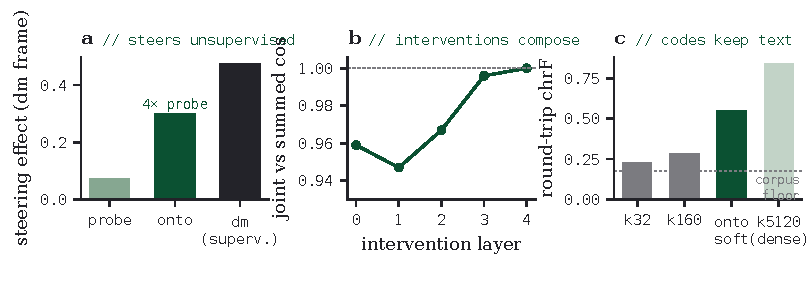
\includegraphics[width=\linewidth]{figures/fig-teaser.pdf}
\caption[The steering primitive, measured]{The softmax Ontologizer's
steering primitive, measured. (a) Forcing an entry moves decodes along
the supervised difference-of-means direction $0.64\times$ as far as
supervised steering itself and $4\times$ as far as probe directions
(\texttt{resid\_nc\_hm}; Table~\ref{tab:steer-overlay}). (b) Joint
two-head interventions point where the summed single interventions point,
exactly in the final layer (\texttt{resid\_nc}; Section~\ref{sec:formal}).
(c) The sparse SAEs' codes lose most text before any intervention
(round-trip chrF 0.23--0.28 against a 0.18 corpus floor) while the soft
code keeps it (0.55); the dense \texttt{k5120} keeps more but is not a
sparse code (Appendix~\ref{sec:textfid}).}
\label{fig:teaser}
\end{figure}

\subsection{Disjoint support}
\label{sec:intro-disjoint}

Concatenated heads (\texttt{ConcatDictBlock}) give each head its own block
of the dictionary's coordinates, so the atoms of different heads have
disjoint supports by construction. Disjoint support is the strong form of
orthogonality: for non-negative atoms the two coincide
(Eq.~\eqref{eq:disjoint}), while signed vectors can be orthogonal by
cancellation and share every coordinate. Summed heads can only be asked
for it, and they do not deliver it: no trained summed model partitions its
coordinates between heads, and penalizing the overlap on GPT-2 produced a
partition only by moving atom energy into directions the decoder discards
or shrinks, where reconstruction cannot see it (Section~\ref{sec:disjoint},
Appendix~\ref{sec:support}). Disjoint support bears on each of the four
problems above, though unequally. In each case the guarantee holds between
the heads of one layer and in the dictionary; what reaches the output
passes through a shared decoder, which in general maps the heads' blocks
onto overlapping subspaces.

\paragraph{Disentanglement.}
Absorption needs two things: a general latent that switches off where a
specific one fires, and a specific latent whose direction takes over the
general one's. The head structure removes the first, since every head
writes on every input, choosing among its entries, and so cannot fall
silent where its feature applies. Disjoint support removes the second: no entry of one
head can carry a component of another head's block. Feature composition
is discouraged rather than excluded. Heads already make the code factorial,
$k^h$ codes from $hk$ atoms, so concepts that vary independently can take
separate heads, and theory says when an efficient code would put them
there. Under a quadratic cost on activity and a bound on the
weights~\cite{whittington2023,dorrell2025}, a non-negative code gives two
variables disjoint supports when their joint range is spread enough,
roughly when every combination of their extreme values
occurs~\cite{dorrell2025}. On SONAR the data meet that condition: of the
entry pairs of two heads that independence predicts at least ten times,
at most 0.24\% never occur in any layer of a SONAR model. The summed
models carry no such cost and do not partition
(Appendix~\ref{sec:support}); concatenation imposes the partition by
construction. Nothing yet forces a head to hold one concept rather than a
conjunction of two. Nor can any method that sees only the data recover its
factors without inductive biases, on the model and on the data, that
match~\cite{locatello2019}. The heads are such a bias, and
Section~\ref{sec:seeds} measures how far it reaches.

\paragraph{Causality.}
An SAE's steering is unclean partly because its decoder directions crowd
one another~\cite{duan2026}. Between heads, nothing crowds in the
dictionary. Forcing a head's entry rewrites only that head's block of the
layer's output, orthogonal to everything the other heads of the layer
write, so interventions on different heads move the output along
orthogonal directions and each head's contribution can be read off its
own block. Summed heads also compose additively, by linearity, but their
writes overlap, so one head's contribution cannot be read apart from the
others'. What disjoint support does not govern is how the other heads
read a stepped input. Measured on the summed models by re-encoding, an
input-space step moves as many other heads as a random step of its
length, because the heads sit almost on their decision boundaries and
downstream layers reclassify a changed residual
(Section~\ref{sec:entangle}). A disjoint write removes neither cause.

\paragraph{Closed form.}
A static reading of the dictionary, which interprets a head from its
atoms without data, needs heads that own disjoint coordinates as a
property of the weights, for every input rather than on the data measured
(Section~\ref{sec:disjoint}). In the summed models that premise fails:
each head's usage covers 52--98\% of the coordinates. Concatenated heads
supply it, and when each head's decoder block has full column rank, every
part of a head's atoms reaches the output, unlike the partitions the
overlap penalty produced (Appendices~\ref{sec:support}
and~\ref{sec:concatgeom}). It is a premise, not yet a reading:
decoding atoms through the paired decoder has not described what an entry
does in the models scored so far, none of them with concatenated heads
(Section~\ref{sec:autointerp}).

\paragraph{Cost.}
Disjoint support does least here. Concatenation divides the dictionary
among the heads, so at matched width $e$ each head stores $k$ atoms of
$e/h$ coordinates rather than $e$, $h$ times fewer dictionary parameters,
and a hard code's dictionary step is $h$ lookups that together write one
$e$-vector. But the classifier still scores all $hk$ entries for every
input, as an SAE scores all of its latents, so the forward pass is no
cheaper on the encoder side. Narrow blocks also cost reconstruction. At
$d_{\mathrm{head}}{=}k$, where each head's block is just wide enough for
its atoms, concatenated heads had the worst held-out error of the GPT-2
orthant arms ($\fvu$ $0.416$ against $0.154$--$0.293$;
Table~\ref{tab:orthant}); orthogonal atoms within a head need one
coordinate each there (Appendix~\ref{sec:concatgeom}).

\subsection{This document}

This document is the working record of that program. It compares a
softmax (soft-code) Ontologizer and a straight-through (hard-code) arm
against $\topk$ SAEs on SONAR sentence embeddings under the same whitened
objective, and the hard code on GPT-2 small residuals.
Section~\ref{sec:background} places the architecture among its nearest
neighbors and Section~\ref{sec:frame} states what the evaluation asks;
the architecture follows in Section~\ref{sec:methods} and the results in
Sections~\ref{sec:results}--\ref{sec:geom}.

\section{Background}
\label{sec:background}

No single line of prior work covers this combination; each commitment has
a nearest neighbor.

\paragraph{Quantizers and discrete latents.}
A \texttt{DictBlock} layer --- $h$ heads, each a softmax over $k$ entries,
their atoms summed --- is a soft additive quantizer~\cite{babenko2014}, the
generalization of product quantization~\cite{jegou2011} in which every
codebook spans the whole space rather than its own block of coordinates
(\texttt{ConcatDictBlock} is a product quantizer in the dictionary space).
Composite quantization~\cite{zhang2014composite} lies between the two: it
holds the summed inner products between different codebooks' codewords at
a constant, which product quantization's disjoint blocks fix at zero, and
optimized product quantization~\cite{ge2014} learns the rotation that sets
the blocks.
In dictionary-learning terms a hard head is vector quantization, one atom
at unit coefficient, and a sum of heads lies between vector quantization
and free sparse coding, with exactly one unit-coefficient atom per
codebook; under the gain--shape split (Eq.~\eqref{eq:y_norm}) each layer
is gain--shape VQ, its one coefficient the residual's measured norm rather
than a quantized index~\cite{aharon2006}.
The residual layer stack is a softmax relaxation of residual (multi-stage)
VQ, the quantizer of neural codecs such as SoundStream~\cite{zeghidour2021},
which picks each stage's code by nearest neighbor and judges codes only by
rate and perceived quality, never by what a codeword means; residual VQ has
also been applied to SONAR space itself, with 64 codebooks of 8192
entries~\cite{lcmteam2024largeconceptmodelslanguage}. The straight-through
arm (Section~\ref{sec:ste}) makes the analogy literal: with an argmax
forward and the softmax's gradient in the backward pass --- the
straight-through estimator~\cite{bengio2013} in its categorical
form~\cite{jang2017} --- it is a residual additive quantizer with
non-negative atoms, whose codewords are picked by learned classifiers
rather than by nearest-codeword search. Vectors of categorical variables
trained with straight-through gradients are also the latent state of
discrete world models~\cite{hafner2021,hafner2023}, which sample each
categorical from the softmax the backward differentiates rather than take
its argmax (DreamerV3 also mixes 1\% uniform into it~\cite{hafner2023});
there the codes are compressed state, never read as features. Codebook Features~\cite{tamkin2023} is the
closest interpretability ancestor: it finetunes VQ bottlenecks into
a network, one codebook per attention head ahead of the shared output
projection (in effect \texttt{ConcatDictBlock} with its shared decoder),
and steers by substituting codes, including swapping one state's code for
another's in a synthetic finite-state task. But its codes are chosen by
cosine similarity to the codes themselves rather than by a classifier,
read one at a time as present-or-absent features, and scored on their
target alone, with no defined set of operations and no measure of what
else an intervention changes.

\paragraph{Routed and mixture-of-experts dictionaries.}
Switch SAEs~\cite{mudide2025} route each activation to one of several
expert $\topk$ SAEs to cut training compute;
routing gathers similar inputs, and experts duplicate some features
(5--10\% of decoder directions have a near-copy in another expert), which
Xu et al.\ describe as experts collapsing into redundant ensembles and
counter by activating several experts per
input~\cite{xu2025redundancydiversespecializedmultiexpert}. A head layer is
the dual arrangement --- every head fires, choosing one entry --- and the
hard stack's heads partition near-independently
(Figure~\ref{fig:headnmi}), while in the reference softmax model a head's
decode directions repel (Section~\ref{sec:prelim-orth}): a head there is a
contrast set rather than the coherent cluster that MoE work counts as a
specialized expert. MoEfication~\cite{zhang2022} supplies the frame's name,
but its experts are found post hoc in already-trained layers and several
are active per input; a head's entries instead exclude one another, and
the partition is the training objective's own discovery.

\paragraph{Deep clustering.}
Each head is a $k$-way classifier trained without labels, the setting of
deep clustering, which supplies two of the objective's terms. The
batch-mean entropy term $\mathrm{KL}_m$ (Eq.~\eqref{eq:KL}) is the
anti-collapse term of contrastive clustering~\cite{li2021cc} and
SCAN~\cite{vangansbeke2020scan}, which keeps a clusterer from assigning
most inputs to a few clusters, and the partition-consensus statistic
$\mathrm{KL}_{\mathrm{pwak}}$ (Eq.~\eqref{eq:stats}) pulls each
assignment toward a stop-gradient average of its neighbors', in the line
of DEC's self-training target~\cite{xie2016dec} and SCAN's neighbor
agreement. Those methods learn one clustering of a learned embedding and
are judged by agreement with class labels; here many heads partition a
fixed embedding at once, trained only through reconstruction, and the
partitions are the code.

\paragraph{Structured SAEs.}
Sparse autoencoders recover features in superposition~\cite{elhage2022}
as sparse combinations of directions from an overcomplete
dictionary~\cite{cunningham2023,bricken2023}; the $\topk$ baselines here
are k-sparse autoencoders~\cite{makhzani2014} trained as in Gao et
al.~\cite{gao2024}. The field's main structure axis is nesting by scale:
Matryoshka SAEs~\cite{bussmann2025} carry the nested loss of Matryoshka
representation learning~\cite{kusupati2022} into a dictionary to curb
feature absorption~\cite{chanin2025}, and Tree SAEs~\cite{cao2026} learn
explicit parent--child pairs by gating each child latent on an assigned
parent. Grouping is a second axis: subspace-aware SAEs~\cite{dalili2026}
tie latents into rank-$r$ blocks and sparsify across blocks, so that a
group is a subspace with free signed coordinates, and
OrtSAEs~\cite{korznikov2025} penalize each decoder direction's cosine with
its nearest neighbor. Rung 3 (\texttt{k32\_p5}) imports the Matryoshka
nested-prefix loss into the ladder, with five equal blocks rather than the
doubling block sizes of~\cite{bussmann2025}, a log spacing that Matryoshka
representation learning found better than uniform~\cite{kusupati2022}.
The Ontologizer's axis is instead \emph{partition into exhaustive,
mutually exclusive heads}, and the geometry such heads ask for has a
theory: in Elhage et al.'s toy models, a set of features of which only one
is active at a time shares a subspace with negative interference inside
it, while separate sets take mutually orthogonal
subspaces~\cite{elhage2022}. A head imposes the first arrangement by
construction and asks for the second (Section~\ref{sec:disjoint}).
Outside dictionary learning, Huang and Hahn~\cite{huang2025decomposing}
partition a residual stream without supervision into mutually independent
orthogonal subspaces, on the hypothesis that each holds a group of
mutually exclusive features; their subspaces carry continuous activations
where a head names one of $k$ values. Post hoc, co-occurring latents of
LLM SAEs cluster in decoder space by document genre~\cite{li2024geometry},
the co-firing structure \texttt{headstruct.py} finds among SONAR SAE
latents in place of categorical groups (Appendix~\ref{sec:categorical}).
Each of these asks whether an architectural commitment buys
interpretability that code density alone does not explain. The autointerp
results below answer ``not per-latent describability''; the
description-coherence view is where the partition begins to pay,
suggestively and on the one Ontologizer it scores.

\paragraph{Embedding-space substrate.}
SAEs over dense text embeddings have become an active line of work:
interpreting and discretizing dense-retrieval
embeddings~\cite{park2025decodingdenseembeddingssparse} and aligning
sentence-embedding features with human concepts to steer
retrieval~\cite{shin2026aligningsentenceembeddingshuman}, while a
data-analysis toolkit builds interpretable document embeddings from a
token-level LLM SAE instead~\cite{jiang2026interpretableembeddingssparseautoencoders}.
All three rely on single-layer SAEs, $\topk$ or its BatchTopK variant, the
embedding SAEs on English retrieval encoders. None addresses SONAR, where
the stakes are higher --- Large Concept Models generate directly in SONAR
space~\cite{lcmteam2024largeconceptmodelslanguage} --- and where the paired
M2M100 decoder reads reconstructions and interventions back as text
without a trained inverter. Inverting a pooled sentence embedding
otherwise needs one, which recovers exact text only by iteratively
re-embedding and correcting its own
decodes~\cite{morris2023textembeddingsrevealalmost}; exact training-free
inversion is known only from a causal language model's per-token
states~\cite{nikolaou2025}, which a bidirectional, mean-pooled encoder
such as SONAR's does not provide. \texttt{textfid.py} and
\texttt{steerfid.py} decode in a single greedy pass through a decoder that
paraphrases and is fragile to small
perturbations~\cite{sonar,lcmteam2024largeconceptmodelslanguage}, so their
text-space numbers are lower bounds (Appendix~\ref{sec:steertext}).

\paragraph{Evaluation stance.}
SAEBench~\cite{karvonen2025} motivates judging a dictionary with many
instruments rather than by reconstruction at fixed sparsity; of its eight
metrics the battery adapts three to SONAR (a loss-recovered analogue
through the paired decoder, \texttt{textfid.py}; LLM-judged detection,
\texttt{autointerp.py}; $k_{\mathrm{probe}}$-sparse probing on 86
language labels, \texttt{langprobe.py}) and omits absorption, RAVEL,
unlearning, SCR and TPP. Description scoring uses the detection task of
the scaled autointerp pipeline~\cite{paulo2025}; unlike that pipeline we
score positives ranked just below the describing examples and report F1
rather than balanced accuracy, so our numbers are not on its scale.
Capacity is compared in bits rather than $\mathrm{L0}$, as
MDL-SAEs~\cite{ayonrinde2024} argue it should be, since an $\mathrm{L0}$
axis rewards ever wider dictionaries with ever fewer active latents; their
description length, summed per-latent usage entropy, is the realized-bits
estimator applied here to heads (Eq.~\eqref{eq:realized}).
AxBench~\cite{wu2025axbenchsteeringllmssimple} found that, averaged over
four Gemma-2 sites, prompting and then finetuning steer better than every
representation-based method. Among single directions only the difference
of means beats SAE latents, while a linear probe that ties the best
detectors steers worse than they do, and SAE latents chosen by their
autointerp labels also trail at concept detection. Detection and steering
dissociate, which supports judging a dictionary by what its directions do
--- the niche of \texttt{steerfid.py}'s
effect-against-collateral design at matched magnitude, which follows
Cunningham et al.'s scoring of feature edits against edit
magnitude~\cite{cunningham2023}, where AxBench instead tunes each method's
strength on held-out prompts. Song et
al.~\cite{song2025positionmechanisticinterpretabilityprioritize} argue
that run-to-run feature consistency should be an essential SAE evaluation
criterion, measured as the mean absolute cosine between decoder directions
matched one-to-one across seeds; \texttt{partition.py}'s Hungarian-matched
head NMI is its partition-level analogue for classifier heads, and
\texttt{splitting.py}'s match fractions a thresholded, activation-based
one. Wang et al.~\cite{wang2024} measure the same property as each latent's
maximum activation correlation with any latent of another run, against
model-seed and SAE-seed skylines. Korznikov et al.~\cite{korznikov2026}
retrain SAEs with the decoder frozen at a random initialization, or held
near it, or with the encoder frozen at random, and find them within a few
points of trained SAEs on autointerp, single-latent sparse probing and
RAVEL; the nulls here permute a trained model's own entries, latents or
rows, and do not measure what training adds over random components.
Decoding parameter directions through the paired decoder, to see whether
features can name themselves from weights alone, is a closed-form
instance of dataset-free feature synthesis, whose evaluation against
implanted ground truth finds that even the best such tools help humans
identify a planted trigger less than half the time~\cite{casper2023};
here the weights fail too. Two pieces have, to our knowledge, no close
analog: reading per-head routing as contrastive classification with a
causal intervention interface, and per-group coherence tests against
size-matched draws from the same dictionary, applied to trained heads and
to judge-written description texts as well as to geometry. Li et
al.~\cite{li2024geometry} test whole co-occurrence clusterings of SAE
latents against permuted labels.

\section{Evaluation frame}
\label{sec:frame}

The comparisons below were largely built on SAE-native terms ---
per-feature monosemanticity, sparse probing, reconstruction at matched
sparsity --- and we report them unchanged. But the Ontologizer's goal is
not a monosemantic dictionary. It is an \emph{unsupervised generator of
steering vectors}: each head is trained only by reconstruction pressure,
the hope is that a series of such classifiers finds the most natural
contrastive clusters in the embedding space, and within-head entry swaps
are the steering primitive (forcing head $i$ from its argmax entry to
entry $j'$ moves the decode along exactly the dimension head $i$
classifies).

Under this frame the evaluation questions are: (a)~what does contrast-set
structure cost in reconstruction (the Pareto and ladder); (b)~do trained
heads actually behave as contrastive classifiers (categorical form,
semantic anti-coherence); (c)~are the learned tasks \emph{natural} ---
nameable, stable across runs, aligned with generative factors of the data
(seed reproducibility, language and topic alignment); and (d)~is the
steering primitive good --- consistent effect, low collateral, at least
matching supervised diff-of-means vectors and SAE decoder-direction addition
(steering fidelity). Metrics that ask whether \emph{individual latents}
are concept-aligned remain informative about the SAE side but are the
wrong lens for classifier codes, and we flag them as such where they
appear. Figure~\ref{fig:teaser} shows the softmax Ontologizer on three
of question (d)'s criteria; the hard code steers less reliably than the
soft one (Section~\ref{sec:steer}).

Question (c) has a prerequisite that the original battery took for
granted: a head can only be named if it is the same head on every run.
Section~\ref{sec:seeds} tests that directly and finds it holds only
partly, and only in the first layer, which conditions every per-head
result in this document.


\section{Methods}
\label{sec:methods}

\subsection{Architecture}
\label{sec:arch}
We propose a novel method which encodes samples as classifications
mapped to contrastive vectors. This directly constrains a model's
representations. Moreover, classifications can natively be used for
steering. Appendix~\ref{app:notation} collects the notation.

The model (Figure~\ref{fig:onto-stack}) consists of $l$ $\dictenc$
layers writing into a shared residual accumulator, decoded by a single
linear map. Each layer (Figure~\ref{fig:dictenc}) is composed of a
classifier layer followed by a dictionary layer. 
The classifier splits the input into $h$ independent soft assignment
vectors, each over one head's $k$ entries.
The dictionary maps each entry to an atom.
Each layer writes a weighted average of these atoms to an accumulator.
After each layer the accumulator is decoded, and the residual is passed
on: layer $\ell$ receives $\mathbf{x} - \mathrm{dec}(\mathbf{r}_\ell)$,
where $\mathbf{r}_\ell$ holds the $\ell$ layers before it.
Deep supervision~\cite{lee2015deeply} constrains every prefix of the
stack to reconstruct the input, and because each layer reads the residual,
what earlier layers encode is gone from what later layers see: the code is
a successive refinement, coarse-to-fine in distortion. Unlike a Tree
SAE~\cite{cao2026}, no later entry is tied to an earlier one, so whether
the code is also coarse-to-fine in concept is an empirical question.

Because entries within a head are mutually exclusive rather than independent,
each dictionary head serves as a contrastive set.
An auxiliary loss term minimizing the heads' support overlap $\omega$
(Eq.~\eqref{eq:support}) pushes each head onto its own coordinates of the
dictionary space (Figure~\ref{fig:head-simplex}).
Because each head returns a convex combination of its atoms, a head's
outputs fill the simplex the atoms span (Section~\ref{sec:dict}).



%The mechanism is small enough to quote, excerpted from
%\texttt{dictblock.py} with dtype casts, intervention plumbing, and two
%live no-ops --- the identity output activation and the optional per-head
%scaling vector --- removed:
%
%\begin{lstlisting}[language=Python]
%def cluster(self, K, temperature=1.0):   # logits -> classifications,
%    return softmax(K / temperature)      # per head, over k entries
%
%def dicts(self):                         # abs() prevents subtractive
%    return jnp.abs(self.weights)         # ontofeatures; (h, k, d)
%
%def fwd(self, P):                        # convex combination per head,
%    return jnp.einsum("...hk,hkd->...d", # summed over heads
%                      P, self.dicts())
%
%def __call__(self, K, temperature=1.0):
%    return self.fwd(self.cluster(K, temperature))
%\end{lstlisting}

\begin{figure}[tp]
\centering
\resizebox{\linewidth}{!}{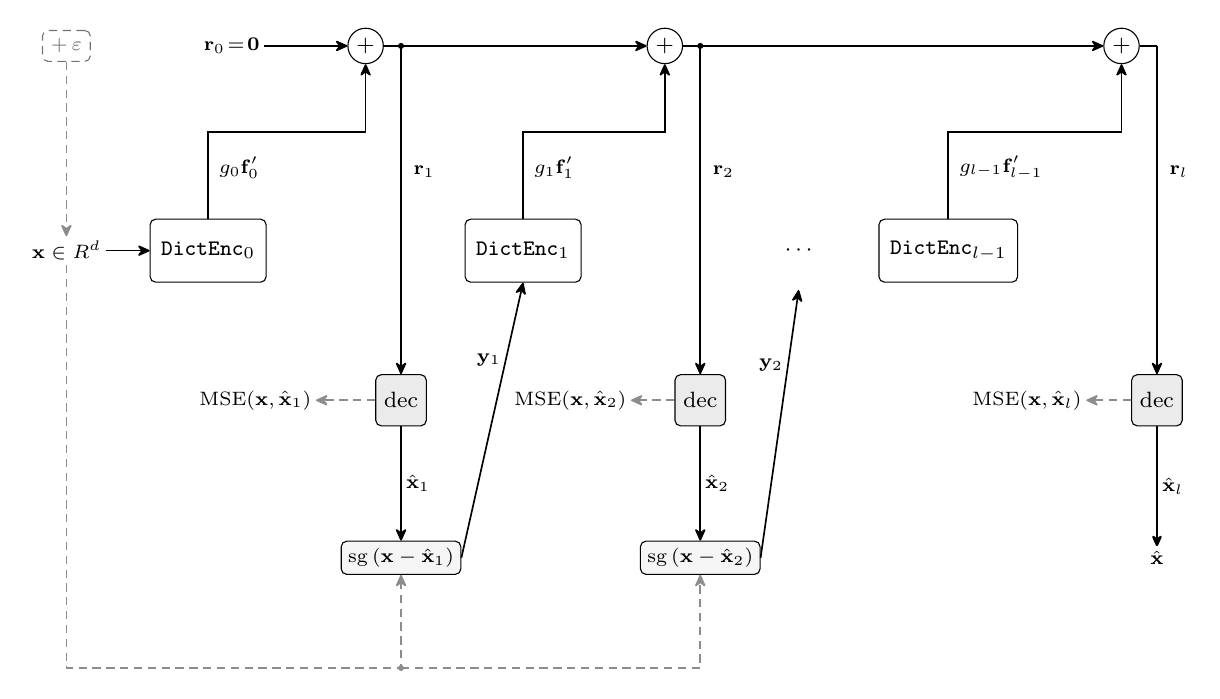
\begin{tikzpicture}[
    font=\footnotesize,
    >={Stealth[round,length=1.8mm,width=1.6mm]},
    blk/.style={draw, rounded corners=2pt, align=center,
                minimum height=8mm, inner xsep=4pt},
    hook/.style={draw, rounded corners=2pt, densely dashed, align=center,
                 inner sep=3pt, font=\scriptsize, black!55},
    dec/.style={draw, rounded corners=2pt, fill=black!8,
                minimum height=6.5mm, inner xsep=3pt},
    cond/.style={draw, rounded corners=2pt, fill=black!4, align=center,
                 inner sep=2.5pt, font=\scriptsize},
    add/.style={draw, circle, minimum size=4.5mm, inner sep=0pt},
    lab/.style={inner sep=1.5pt, font=\scriptsize},
    sig/.style={->, semithick},
    aux/.style={->, densely dashed, semithick, black!45},
  ]

  %% ---- layer row --------------------------------------------------
  \node[lab] (x)  at (-1.5,0) {$\mathbf{x}\in\mathbb{R}^{d}$};
  \node[blk] (D0) at ( 0.3,0) {$\mathtt{DictEnc}_0$};
  \node[blk] (D1) at ( 4.3,0) {$\mathtt{DictEnc}_1$};
  \node      (Dd) at ( 7.8,0) {$\cdots$};
  \node[blk] (DL) at ( 9.7,0) {$\mathtt{DictEnc}_{l-1}$};

  \draw[sig] (x) -- (D0);

  \node[hook] (noise) at (-1.5,2.6) {$+\,\varepsilon$};
  \draw[aux] (noise) -- (x);

  %% ---- residual accumulator (top rail, y = 2.6) --------------------
  \node[add] (A0) at ( 2.3,2.6) {$+$};
  \node[add] (A1) at ( 6.1,2.6) {$+$};
  \node[add] (AL) at (11.9,2.6) {$+$};

  \node[lab] (R0) at (0.6,2.6) {$\mathbf{r}_0\!=\!\mathbf{0}$};
  \draw[sig]      (R0) -- (A0);
  \draw[sig]      (A0) -- (A1);
  \draw[sig]      (A1) -- (AL);
  \draw[semithick] (AL) -- (12.35,2.6);

  %\node[lab] at (8.9,3.05) {$\mathbf{r}\in\mathbb{R}^{e}$: residual accumulator};

  %% ---- per-layer contributions g_l f'_l (enter from below) ----------
  \draw[sig] (D0.north) -- ++(0,1.1) -| (A0.south);
  \draw[sig] (D1.north) -- ++(0,1.1) -| (A1.south);
  \draw[sig] (DL.north) -- ++(0,1.1) -| (AL.south);
  \node[lab,anchor=west] at (0.38,1.05) {$g_0\mathbf{f}'_0$};
  \node[lab,anchor=west] at (4.38,1.05) {$g_1\mathbf{f}'_1$};
  \node[lab,anchor=west] at (9.78,1.05) {$g_{l-1}\mathbf{f}'_{l-1}$};

  %% ---- shared decoder, one decode per prefix -----------------------
  \node[dec] (Y1) at ( 2.75,-1.9) {$\mathrm{dec}$};
  \node[dec] (Y2) at ( 6.55,-1.9) {$\mathrm{dec}$};
  \node[dec] (YL) at (12.35,-1.9) {$\mathrm{dec}$};

  \draw[sig] ( 2.75,2.6) -- (Y1.north);
  \draw[sig] ( 6.55,2.6) -- (Y2.north);
  \draw[sig] (12.35,2.6) -- (YL.north);
  \fill ( 2.75,2.6) circle (1.1pt);
  \fill ( 6.55,2.6) circle (1.1pt);

  \node[lab,anchor=west] at ( 2.85,1.0) {$\mathbf{r}_1$};
  \node[lab,anchor=west] at ( 6.65,1.0) {$\mathbf{r}_2$};
  \node[lab,anchor=west] at (12.45,1.0) {$\mathbf{r}_{l}$};

  %% ---- deep supervision --------------------------------------------
  \node[lab] (L1) at ( 0.9,-1.9) {$\mathrm{MSE}(\mathbf{x},\hat{\mathbf{x}}_1)$};
  \node[lab] (L2) at ( 4.9,-1.9) {$\mathrm{MSE}(\mathbf{x},\hat{\mathbf{x}}_2)$};
  \node[lab] (LL) at (10.7,-1.9) {$\mathrm{MSE}(\mathbf{x},\hat{\mathbf{x}}_{l})$};
  \draw[aux] (Y1.west) -- (L1);
  \draw[aux] (Y2.west) -- (L2);
  \draw[aux] (YL.west) -- (LL);

  %% ---- residual forwarding ------------------------------------------
  \node[cond] (C1) at (2.75,-3.9)
  {$\mathrm{sg}\,(\mathbf{x}-\hat{\mathbf{x}}_1)$};
  \node[cond] (C2) at (6.55,-3.9)
  {$\mathrm{sg}\,(\mathbf{x}-\hat{\mathbf{x}}_2)$};
  \draw[sig] (Y1) -- node[right,lab]{$\hat{\mathbf{x}}_1$} (C1);
  \draw[sig] (Y2) -- node[right,lab]{$\hat{\mathbf{x}}_2$} (C2);

  \draw[sig] (C1.east) -- node[left,lab,pos=0.72]{$\mathbf{y}_1$} (D1.south);
  \draw[sig] (C2.east) -- node[left,lab,pos=0.72]{$\mathbf{y}_2$} (7.8,-0.5);

  %% ---- model output --------------------------------------------------
  \node[lab] (out) at (12.35,-3.9) {$\hat{\mathbf{x}}$};
  \draw[sig,thick] (YL) -- node[right,lab]{$\hat{\mathbf{x}}_{l}$} (out);

  %% ---- x broadcast to every conditioning step -------------------------
  \draw[aux] (x.south) -- (-1.5,-5.3) -- (2.75,-5.3) -- (C1.south);
  \draw[aux] (2.75,-5.3) -- (6.55,-5.3) -- (C2.south);
  \fill[black!45] (2.75,-5.3) circle (1.1pt);

\end{tikzpicture}

}
\caption[\texttt{Ontologizer} architecture]{\textbf{\texttt{Ontologizer} architecture.}
	Each \texttt{DictEnc} writes its gain-scaled output
	$g_\ell\mathbf{f}'_\ell$ into a shared accumulator. States count the
	layers applied: layer $\ell$ reads $\mathbf{r}_\ell$ and the residual
	$\mathbf{y}_\ell$, and writes $\mathbf{r}_{\ell+1}$. One decoder serves
	every prefix, and each prefix is scored against $\mathbf{x}$ (deep
	supervision). The dashed input-noise hook is off in every reported
	model. Section~\ref{sec:decoder} gives the equations.}
\label{fig:onto-stack}
\end{figure}

\subsubsection{DictEnc}
\label{sec:dictenc}
Each $\dictenc$ consists of a multihead bilinear classifier
($\bilinearblock$) with weights
$[\mathsf{W}, \mathsf{V}] \in \mathbb{R}^{2 \times h \times k \times d}$
($d+1$ with the constant coordinate of Eq.~\eqref{eq:y_norm})
and a multihead linear dictionary ($\dictblock$)
with weights $\mathsf{D} \in \mathbb{R}^{h \times k \times e}$.
Its input is the residual $\mathbf{y}_\ell$ left by the layers before it
($\mathbf{x}$ itself at layer 0), of which the classifier reads the
shape $\mathbf{u}_\ell$ (Eq.~\eqref{eq:y_norm}).
Algorithm~\ref{alg:dictenc} gives one layer's training pass, and
Algorithm~\ref{alg:ontologizer} the stack and its loss.

\begin{algorithm}[tp]
	\caption{$\dictenc$, one layer, in training (\texttt{DictEnc.withStats}).
	Without the router, $\Gamma$ is all ones and $\mathrm{L1}_S = 0$; without
	fibers there are no coordinates $\mathsf{C}$; without
	\texttt{resid\_gain} the input is not split and $g = 1$.}
	\label{alg:dictenc}
	\DontPrintSemicolon

	\KwIn{accumulator $R \in \mathbb{R}^{b \times e}$; layer input
		$E \in \mathbb{R}^{b \times d'}$, whose row $n$ is
		$[\mathbf{y}_n;\, \mathbf{1}_{n_{\mathrm{const}}}]$: the varying
		part $\mathbf{y}_n$ (the encoded input at layer 0, the residual
		above) and $n_{\mathrm{const}}$ constant coordinates
		(\texttt{resid\_const})}
	\KwData{bilinear classifier (Eq.~\eqref{eq:bilinearblock}); router
		(\texttt{scaled}); fiber readouts $A_i \in \mathbb{R}^{r \times d'}$;
		$\dictblock$ (Algorithm~\ref{alg:dictblock})}
	\Hyper{logit noise $\sigma_K$; fiber bound $\beta$; the
		$\dictblock$ hyperparameters}
	\KwOut{accumulator $R$; assignments
		$\mathsf{P} \in \mathbb{R}^{b \times h \times k}$; statistics
		row $\boldsymbol{\psi}$ (Eq.~\eqref{eq:stats})}

	\Begin{
		$g_n \leftarrow \mathrm{sg}\big[\lVert \mathbf{y}_n\rVert\big]$;\quad
			$\mathbf{u}_n \leftarrow \big[\mathbf{y}_n/g_n;\,
			\mathbf{1}_{n_{\mathrm{const}}}\big]$
			\tcp*{gain and shape}
		$\mathsf{K}, \mathrm{L1}_K \leftarrow
			\mathrm{classifier}(\mathbf{u}_{1:b})$
			\tcp*{L1 of the gate factor}
		$\mathsf{K} \leftarrow \mathrm{noise}_K(\mathsf{K})$
			\tcp*{Eq.~\eqref{eq:noise_normal} or~\eqref{eq:noise_batchnorm}}
		\eIf{router}{
			$\Gamma, \mathrm{L1}_S \leftarrow \mathrm{router}(\mathbf{u}_{1:b})$;\quad
				$\Gamma \leftarrow \lvert \Gamma \rvert$
				\tcp*{unless \texttt{router\_signed}}
		}{
			$\Gamma \leftarrow \mathbf{1}$;\quad $\mathrm{L1}_S \leftarrow 0$\;
		}
		$\mathbf{c}_{ni} \leftarrow \beta \tanh(A_i \mathbf{u}_n / \beta)$
			\tcp*{fiber coordinates, Eq.~\eqref{eq:fiber}}
		$F', \mathsf{P}, (\mathrm{L1}, H, \mathrm{cossim}_b,
			\mathbb{E}_i\kappa_i, \max_i \kappa_i, \mathrm{KL}_m, \omega)
			\leftarrow \dictblock(\mathsf{K}, \Gamma, \mathsf{C})$\;
		$\mathrm{KL}_{\mathrm{pwak}}, \mathrm{L2}_{\mathrm{pwak}}
			\leftarrow \mathrm{pwak}(\mathsf{P}, \mathbf{u}_{1:b})$
			\tcp*{zero unless enabled}
		$\mathbf{r}_n \leftarrow \mathbf{r}_n + g_n\,\mathbf{f}'_n$
			\tcp*{row $n$ of $R$: the contribution, at the input's gain}
		\Return{$R$, $\mathsf{P}$,
			$\boldsymbol{\psi} = (\mathrm{L1}_K, \mathrm{L1}, H, \mathrm{cossim}_b,
			\mathbb{E}_i\kappa_i, \max_i \kappa_i, \mathrm{KL}_m,
			\mathrm{KL}_{\mathrm{pwak}}, \mathrm{L2}_{\mathrm{pwak}},
			\mathrm{L1}_S, \omega)$}\;
	}
\end{algorithm}


\begin{figure}[tp]
\centering
\resizebox{\linewidth}{!}{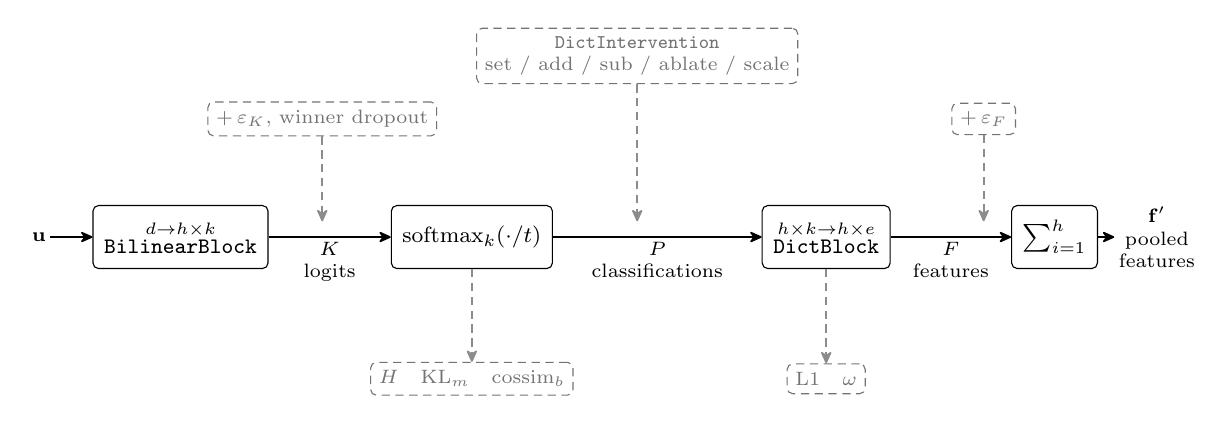
\begin{tikzpicture}[
    font=\footnotesize,
    >={Stealth[round,length=1.8mm,width=1.6mm]},
    blk/.style={draw, rounded corners=2pt, align=center,
                minimum height=8mm, inner xsep=4pt},
    hook/.style={draw, rounded corners=2pt, densely dashed, align=center,
                 inner sep=3pt, font=\scriptsize, black!55},
    lab/.style={inner sep=1.5pt, font=\scriptsize, align=center},
    sig/.style={->, semithick, align=center},
    aux/.style={->, densely dashed, semithick, black!45},
  ]

  %% ---- main chain ----------------------------------------------------
  \node[lab] (E)  at (-0.6,0) {$\mathbf{u}$};
  \node[blk] (CL) at ( 1.2,0) {$\bilinearblock^{d \to h \times k}$};
  \node[blk] (SM) at ( 4.9,0) {$\mathrm{softmax}_k(\cdot/t)$};
  \node[blk] (DB) at ( 9.4,0) {$\dictblock^{h \times k \to h \times e}$};
  \node[blk] (SU) at (12.3,0) {$\sum^{h}_{i=1}$};
  \node[lab] (F)  at (13.6,0) {$\mathbf{f}'$\\ pooled\\ features};

  \draw[sig] (E)  -- (CL);
  \draw[sig] (CL) -- node[below,lab]{$K$\\ logits}   (SM);
  \draw[sig] (SM) -- node[below,lab]{$P$\\ classifications}   (DB);
  \draw[sig] (DB) -- node[below,lab]{$F$\\ features} (SU);
  \draw[sig] (SU) -- (F);

  %% ---- training-time hooks and the intervention interface (above) ----
  \node[hook] (nk) at (3.0,1.5) {$+\,\varepsilon_K$,\ winner dropout};
  \node[hook] (iv) at (7.0,2.3) {\texttt{DictIntervention}\\
                                 set / add / sub / ablate / scale};
  \node[hook] (nf) at (11.4,1.5) {$+\,\varepsilon_F$};
  \draw[aux] (nk) -- (3.0,0.20);
  \draw[aux] (iv) -- (7.0,0.20);
  \draw[aux] (nf) -- (11.4,0.20);

  %% ---- where each regulariser attaches (below) -----------------------
  \node[hook] (lp) at (4.9,-1.8)
    {$H$\quad $\mathrm{KL}_m$\quad $\mathrm{cossim}_b$};
  \node[hook] (lf) at (9.4,-1.8)
    {$\mathrm{L1}$\quad $\omega$};
  \draw[aux] (SM.south) -- (lp);
  \draw[aux] (DB.south) -- (lf);

\end{tikzpicture}

}
\caption[\texttt{DictEnc} architecture]{\textbf{\texttt{DictEnc} architecture.}
	A bilinear classifier reads the layer's shape $\mathbf{u}$ and
	returns logits $K$; the assignments $P = \mathrm{softmax}_k(K/t)$
	select atoms from the dictionary, and the per-head outputs $F$ are
	pooled into $\mathbf{f}'$. Dashed boxes above an arrow perturb it in
	training or carry an intervention; dashed boxes below are statistics,
	usable as auxiliary losses (Sections~\ref{sec:bilinear}--\ref{sec:dict}).}
\label{fig:dictenc}
\end{figure}

\subsubsection{Classifier}
\label{sec:bilinear}
A $\bilinearblock$ accepts an input $\mathbf{x} \in \mathbb{R}^d$ (in a
layer, the shape $\mathbf{u}_\ell$).
It returns logits $K \in \mathbb{R}^{h \times k}$ given by

\begin{equation}
	\bilinearblock([\mathsf{W},\mathsf{V}],\mathbf{x}) :=
	\left(\sum^{d}_{q=1}W_{\cdot,\cdot,q}\,x_q\right)
	 \odot \left(\sum^{d}_{q=1}V_{\cdot,\cdot,q}\,x_q\right)
	 \label{eq:bilinearblock}
\end{equation}

An optional noise term $\varepsilon_K$ may be added.
Winner dropout sets each head's largest logit to $-\infty$
with probability $p_{\mathrm{drop}}$.

\subsubsection{Assignments}
\label{sec:labels}
Soft assignments $P$ are given by $\mathrm{softmax}_{k}(K/t)$
where $t$ is a temperature hyperparameter. Annealing it sharpens the
assignments; each model's schedule is in Appendix~\ref{app:configs}.
The architecture provides methods for causal interventions on assignments.
From $P$ we collect per-sample entropy $H$, in bits, so a head
saturates at $\log_2 k = 5$ bits,

\begin{equation}
	\mathrm{entropy}_k(\mathbf{p}) :=
	-\sum^{k}_{j=1}p_{j}\log_2 p_{j},
	\qquad
	H := \mathbb{E}_{n}\,\mathbb{E}_{i}\!\left[
	\mathrm{entropy}_k(\mathbf{p}_{ni})\right]
	\label{eq:entropy}
\end{equation}

between-sample similarity $\mathrm{cossim}_b$, the mean absolute cosine
similarity of the per-head features $\mathsf{F}$ over all ordered pairs
of samples,

\begin{equation}
	\mathrm{cossim}_b :=
	\mathbb{E}_{n,n'}\big\lvert
	\cos\angle(\mathbf{f}_{n}, \mathbf{f}_{n'})
	\big\rvert,
	\qquad
	\langle \mathbf{f}_{n}, \mathbf{f}_{n'}\rangle
	= \sum^{h}_{i=1}\gamma_{ni}\gamma_{n'i}\,
	\mathbf{p}_{ni}^{\top}G_{i}\,\mathbf{p}_{n'i}
	\label{eq:cossim_b}
\end{equation}

where $\mathbf{f}_{ni} := \mathsf{F}_{ni\cdot} \in \mathbb{R}^{e}$ is
head $i$'s feature vector for sample $n$,
$\mathbf{f}_n = \map_{i=1}^{h}\mathbf{f}_{ni}$ is their concatenation,
$\gamma_{ni}$ is head $i$'s router scale on sample $n$ (1 without a
router; Section~\ref{sec:router-fiber}), and
$G_i = \lvert D_{i}\rvert \lvert D_{i}\rvert^{\top} \in \mathbb{R}^{k \times k}$
is head $i$'s dictionary Gram, with $D_i := \mathsf{D}_{i\cdot\cdot}$ its
$k \times e$ dictionary. The implementation evaluates
Eq.~\eqref{eq:cossim_b} in entry space through the $G_i$ rather than
materializing $\mathsf{F}$; the two are identical in value and gradient,
but $\mathcal{O}(hk^2e + b^2hk)$ instead of $\mathcal{O}(b^2he)$.

Finally, $\mathrm{KL}_m$ is the divergence of the batch-mean assignment
vector from uniform, in bits, averaged over heads.

\begin{equation}
	\mathrm{KL}_m := \mathbb{E}_{i}\!\left[\log_2 k -
	\mathrm{entropy}_k\!\left(\bar{\mathbf{p}}_i\right)\right],
	\qquad
	\bar{\mathbf{p}}_i := \mathbb{E}_{n}\,[\mathbf{p}_{ni}]
	\label{eq:KL}
\end{equation}

In practice $H$ is not needed, as including a
$\mathrm{cossim}_b$ loss also minimizes $H$.
$\mathrm{KL}_m$ serves to anchor the batch mean of each assignment vector
$\mathbf{p}_{ni}$ to a uniform distribution.
It keeps every entry in use, since a head that collapses onto one entry
pays the full $\log_2 k$ bits, and it is meant to make a uniform
$\mathbf{p}_{ni}$ code correspond to a maximally generic feature vector.

\subsubsection{Dictionary}
\label{sec:dict}
A $\dictblock$ accepts assignments
$P \in \mathbb{R}^{h \times k}$
and returns features $F \in \mathbb{R}^{h \times e}$, whose row
$\mathbf{f}_i$ is head $i$'s output, given by

\begin{equation}
	\dictblock(\mathsf{D},P)_{i\cdot} = \mathbf{f}_i :=
	\sum^{k}_{j=1} p_{ij}\,\mathbf{a}_{ij},
	\qquad
	\mathbf{a}_{ij} := \lvert \mathsf{D}_{ij\cdot}\rvert
	\label{eq:dictblock}
\end{equation}

where the atom $\mathbf{a}_{ij}$ is the absolute value of head $i$'s
dictionary row for entry $j$ ($\mathsf{D}_{ij\cdot}$ itself when the
dictionary is signed). Because atoms are absolute values
and $p_{ij} \in [0,1]$, features are strictly additive. Since each head's
assignment sums to one, $\mathbf{f}_i$ lies in the simplex whose vertices
are the head's atoms (Figure~\ref{fig:head-simplex}), the shape Park et
al.~\cite{park2025} derive for the representation of a categorical
concept: a head's entries are mutually exclusive alternatives, not
independently firing features. The lookup has the form of attention over
the head's own dictionary, a softmax over per-entry scores weighting the
atoms as values~\cite{bahdanau2015,luong2015,vaswani2017}, with scores
computed from the input alone; with a linear classifier it is one update
of a modern Hopfield layer at inverse temperature $1/t$~\cite{ramsauer2021}.
Algorithm~\ref{alg:dictblock} gives the full training pass, with the
regularizing perturbations and statistics around this lookup.

\begin{algorithm}[tp]
	\caption{$\dictblock$ in training (\texttt{DictBlock.withStats}). At
	inference the four stochastic steps (revival, winner dropout, head
	dropout, fiber dropout) and the feature noise are skipped. Every
	statistic is stop-gradiented unless its loss term is enabled.}
	\label{alg:dictblock}
	\DontPrintSemicolon
	\footnotesize

	\KwIn{logits $\mathsf{K} \in \mathbb{R}^{b \times h \times k}$;
		router scales $\Gamma \in \mathbb{R}_{\ge 0}^{b \times h}$ (all ones
		without a router); fiber coordinates
		$\mathsf{C} \in \mathbb{R}^{b \times h \times r}$ (none without
		fibers)}
	\KwData{dictionary $\mathsf{D} \in \mathbb{R}^{h \times k \times e}$;
		fiber bases $U_{ij} \in \mathbb{R}^{e \times r}$}
	\Hyper{temperature $t$; feature noise $\sigma_F$; winner dropout
		$p_{\mathrm{drop}}$; revival rate $p_{\mathrm{rev}}$ and threshold
		$\tau_{\mathrm{rev}}$; head dropout $p_{\mathrm{head}}$; fiber dropout
		$p_{\mathrm{fib}}$; entries kept per head $k_{\mathrm{sel}}$
		($1$ under \texttt{ste}/\texttt{argmax}, $k$ under softmax, and
		the rule's own value under \texttt{top}$k_{\mathrm{sel}}$, e.g.\ 4
		for \texttt{top4})}
	\KwOut{pooled features $F' \in \mathbb{R}^{b \times e}$; assignments
		$\mathsf{P} \in \mathbb{R}^{b \times h \times k}$; statistics
		$(\mathrm{L1}, H, \mathrm{cossim}_b, \mathbb{E}_i\kappa_i,
		\max_i \kappa_i, \mathrm{KL}_m, \omega)$}

	\Begin{
		$\mathbf{a}_{ij} \leftarrow \lvert \mathsf{D}_{ij\cdot} \rvert$
			\tcp*{atoms; $\mathsf{D}_{ij\cdot}$ itself if signed}
		\If(\tcp*[f]{revive starved entries}){$k_{\mathrm{sel}} < k$}{
			$\mathrm{use}_{ij} \leftarrow$ share of rows on which entry $j$
				is among head $i$'s top $k_{\mathrm{sel}}$ logits\;
			\ForEach{$(n,i)$ with probability $p_{\mathrm{rev}}$}{
				draw $j$ uniformly from $\{j : \mathrm{use}_{ij} <
					\tau_{\mathrm{rev}}\,k_{\mathrm{sel}}/k\}$, if any\;
				raise entry $j$'s logit on row $n$ to head $i$'s maximum
					\tcp*{tie the leader}
			}
		}
		each $(n,i)$: $\max_j [\mathsf{K}]_{nij} \leftarrow -\infty$ with probability
			$p_{\mathrm{drop}}$ \tcp*{winner dropout}
		$\mathsf{P} \leftarrow \mathrm{select}_k(\mathsf{K}/t)$
			\tcp*{softmax, \texttt{top}$k_{\mathrm{sel}}$ or straight-through}
		$H \leftarrow \mathbb{E}_{n,i}\,\mathrm{entropy}_k(\mathbf{p}_{ni})$
			\tcp*{Eq.~\eqref{eq:entropy}}
		$\bar{\mathbf{p}}_i \leftarrow \mathrm{sg}[\mathbb{E}_n\,
			\mathbf{p}_{ni}]$ \tcp*{head origin}
		\ForEach(\tcp*[f]{head dropout}){$(n,i)$}{
			$\mathbf{p}'_{ni} \leftarrow \bar{\mathbf{p}}_i$ with
				probability $p_{\mathrm{head}}$, else
				$\bar{\mathbf{p}}_i + (\mathbf{p}_{ni} - \bar{\mathbf{p}}_i)
				/ (1 - p_{\mathrm{head}})$\;
		}
		each $(n,i)$: $\mathbf{c}_{ni} \leftarrow \mathbf{0}$ with
			probability $p_{\mathrm{fib}}$ \tcp*{fiber dropout}
		$\mathbf{f}_{ni} \leftarrow \gamma_{ni} \sum_{j} p'_{nij}\,
			\mathbf{a}_{ij}$ \tcp*{Eq.~\eqref{eq:dictblock}; interventions act
			on $\mathbf{p}'$}
		$\tilde{\mathsf{F}} \leftarrow \mathrm{noise}_{\mathrm{featvar}}
			(\mathsf{F})$ \tcp*{Eq.~\eqref{eq:noise_featvar}}
		$\mathrm{cossim}_b \leftarrow \mathbb{E}_{n,n'}
			\lvert\cos\angle(\mathbf{f}_n, \mathbf{f}_{n'})\rvert$
			\tcp*{Eq.~\eqref{eq:cossim_b}, from $\mathsf{P}$ through the Grams}
		$\kappa_i \leftarrow \mathbb{E}_{j \ne j'}
			\cos\angle(\mathbf{a}_{ij}, \mathbf{a}_{ij'})$
			\tcp*{within-head atom cosine}
		$\mathrm{KL}_m \leftarrow \mathbb{E}_i \left[\log_2 k -
			\mathrm{entropy}_k(\bar{\mathbf{p}}_i)\right]$
			\tcp*{Eq.~\eqref{eq:KL}}
		$\boldsymbol{\pi}_i \leftarrow \sum_j \bar{p}_{ij}\,
			\lvert\mathbf{a}_{ij}\rvert$;\quad
			$\omega \leftarrow \mathbb{E}_{i \ne i'}
			\cos\angle(\boldsymbol{\pi}_i, \boldsymbol{\pi}_{i'})$
			\tcp*{support overlap}
		$\mathrm{L1} \leftarrow \mathbb{E}_n \sum_i
			\lVert \tilde{\mathbf{f}}_{ni} \rVert_1$\;
		$\mathbf{f}'_n \leftarrow \sum_i \tilde{\mathbf{f}}_{ni}$
			\tcp*{concatenated, not summed, under $\mathtt{ConcatDictBlock}$}
		\If(\tcp*[f]{Eq.~\eqref{eq:fiber}, then any norm cap}){fibers}{
			$\mathbf{f}'_n \leftarrow \mathbf{f}'_n + \sum_i \gamma_{ni}
				\sum_j p'_{nij}\,U_{ij}\,\mathbf{c}_{ni}$\;
		}
		\Return{$F'$, $\mathsf{P}$,
			$(\mathrm{L1}, H, \mathrm{cossim}_b, \mathbb{E}_i\kappa_i,
			\max_i \kappa_i, \mathrm{KL}_m, \omega)$}\;
	}
\end{algorithm}


From the assignments and the atoms we collect the heads' support overlap
$\omega$, the mean cosine over ordered pairs of distinct heads between
their usage-weighted coordinate profiles $\boldsymbol{\pi}_i$,

\begin{equation}
	\boldsymbol{\pi}_i := \sum^{k}_{j=1} \bar{p}_{ij}\,
	\lvert \mathbf{a}_{ij}\rvert,
	\qquad
	\omega := \mathbb{E}_{i \neq i'}\,
	\frac{\langle \boldsymbol{\pi}_i, \boldsymbol{\pi}_{i'}\rangle}
	     {\lVert \boldsymbol{\pi}_i\rVert \lVert \boldsymbol{\pi}_{i'}\rVert}
	\label{eq:support}
\end{equation}

with $\bar{\mathbf{p}}_i$ the batch-mean assignment of
Eq.~\eqref{eq:KL}. The overlap is zero exactly when no two heads share
a coordinate of the dictionary space and one when every head uses the
same coordinates in the same proportions (Section~\ref{sec:disjoint}). It
costs
$\mathcal{O}(hke + h^2e)$, independent of the batch. Weighting by usage
keeps dead entries out of it and gives the classifier a gradient path.
Figure~\ref{fig:anatomy} shows the assignments, the atoms and both
cosine statistics for one trained head.
We also collect the sparsity penalty $\mathrm{L1}$ after the noise
$\varepsilon_F$ is added, $\tilde{\mathsf{F}} := \mathsf{F} +
\varepsilon_F$. $\mathrm{L1}$ is the batch mean of each sample's norm, so
it does not change with $b$ but scales with $h$ and $e$; its loss weight
is correspondingly small.

\begin{equation}
	\mathrm{L1}(\tilde{\mathsf{F}}) :=
	\frac{1}{b}\sum^{b}_{n=1}\sum^{h}_{i=1}\sum^{e}_{q=1}
	\lvert \tilde{f}_{niq}\rvert
	\label{eq:L1}
\end{equation}

$\mathrm{L1}$ tends to decrease with only $\mathrm{MSE}$ loss, but
incorporating it into the loss speeds up convergence.

\begin{figure}[tp]
\centering
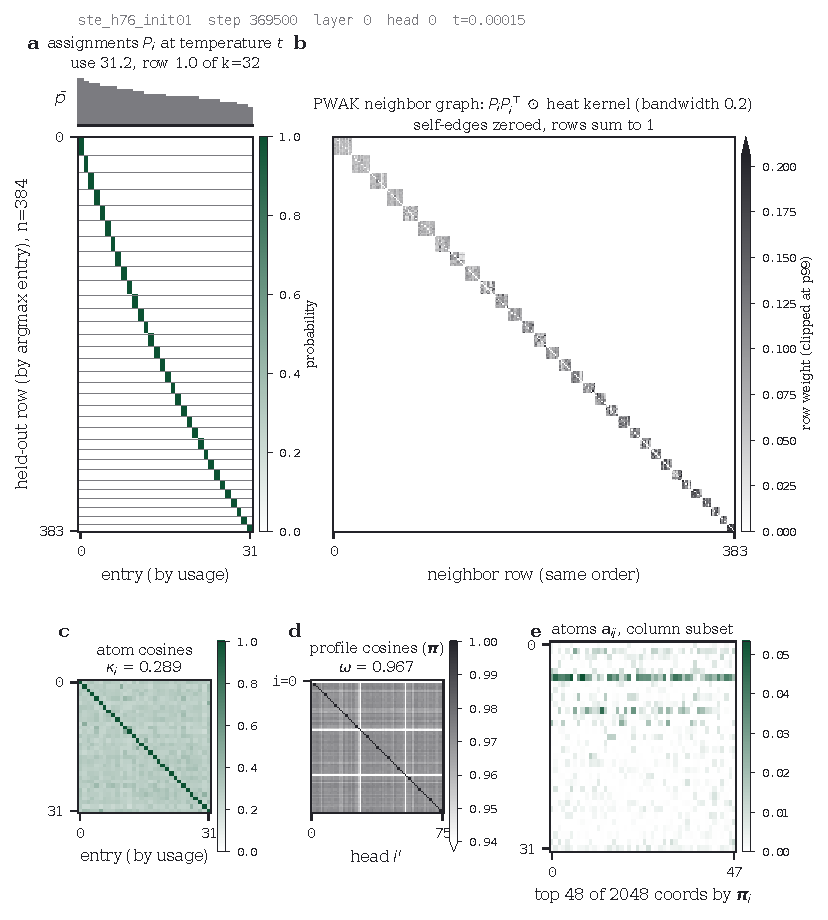
\includegraphics[width=0.85\linewidth]{figures/fig-anatomy.pdf}
\caption[One trained head, block by block]{\textbf{One trained head,
	block by block.} Head $i{=}0$ of layer 0 of the straight-through model
	\texttt{ste\_h76\_init01} (step 369{,}500, $t{=}0.00015$) on $n{=}384$
	rows drawn from the eval tail; one seed. (a) The
	assignments $P_i$, rows sorted by winning entry and entries by mean
	usage $\bar{p}_{ij}$ (bars). ``Use'' is the effective number of
	entries across rows, $\exp H(\bar{\mathbf{p}}_i)$, and ``row'' the
	effective number within a row, the exponential of the mean per-row
	entropy: 31.2 and 1.0 of $k{=}32$, a hard code that uses nearly every
	entry. (b) The neighbor graph that
	$\mathrm{KL}_{\mathrm{pwak}}$ and $\mathrm{L2}_{\mathrm{pwak}}$
	(Eq.~\eqref{eq:stats}) diffuse over, in the same row order: the
	co-assignment matrix $P_iP_i^\top$ times the heat kernel
	$\exp((\langle\mathbf{u}_n,\mathbf{u}_{n'}\rangle - 1)/0.2)$ of the
	layer's shapes without their constant coordinate, self-edges removed
	and each row normalized to sum to one. A hard code makes it
	block-diagonal by cell. This model was not trained with either
	statistic, so the graph is the one they would build, not one that
	shaped it. (c) Cosines between head $i$'s atoms, whose
	off-diagonal mean is $\kappa_i$ (0.289). (d) Cosines between the heads'
	coordinate profiles $\boldsymbol{\pi}$ (Eq.~\eqref{eq:support}) with
	$\bar{\mathbf{p}}$ the mean over the $n$ rows, whose off-diagonal mean
	is $\omega$ (0.967), head $i$'s row outlined. (e) Head $i$'s atoms on
	the 48 of $e{=}2048$ coordinates where $\boldsymbol{\pi}_i$ is largest,
	a column subset rather than a projection. Each block has its own
	scale, white at zero, except (d): $\omega$ is near 1, so its scale
	starts at the 5th percentile of the off-diagonal cosines, and the few
	below it show as white. Figure~\ref{fig:anatomy-softmax} is the same
	head of a softmax model.}
\label{fig:anatomy}
\end{figure}

\paragraph{Disjoint support}
\label{sec:disjoint}
Between heads, orthogonality of non-negative features is not a rotation
constraint but a support-partition constraint. Every $\mathbf{f}_{ni}$
lies in the non-negative orthant of
$\mathbb{R}^e$: the dictionary contributes $\lvert \mathsf{D} \rvert \geq 0$ and
the assignments $P \geq 0$. For non-negative $\mathbf{v}, \mathbf{v}'$ the
inner product $\langle \mathbf{v},\mathbf{v}'\rangle = \sum_q v_q v'_q$ is
a sum of non-negative terms, so it vanishes if and only if every term
does,

\begin{equation}
	\langle \mathbf{v},\mathbf{v}'\rangle = 0
	\iff
	\mathrm{supp}(\mathbf{v}) \cap \mathrm{supp}(\mathbf{v}') = \emptyset
	\label{eq:disjoint}
\end{equation}

Non-negative sparse PCA and orthogonal non-negative matrix factorization
rest on the same fact: orthonormal non-negative components divide the
coordinates among themselves~\cite{zass2006,asteris2015onmf}.
Signed vectors admit no such conclusion: there orthogonality is
cancellation, and two vectors with identical support can be orthogonal.
A penalty on the inner products between groups of signed atoms, such as
the incoherence term Ramirez et al.\ place between per-class
dictionaries~\cite{ramirez2010}, can therefore be met by atoms that share
coordinates. The support overlap of Eq.~\eqref{eq:support} sidesteps this. It
compares the absolute values of the atoms, which have disjoint supports
exactly when they are orthogonal whatever the atoms' signs, so it
measures disjointness under a signed dictionary too; and it is computed
from the atoms and the batch-mean assignment rather than from noised
features, which leave the orthant and the argument with it.

The constraint binds the dictionary, not merely one sample's features.
Because the assignments are a softmax, $p_{nij} > 0$ for every entry, and expanding
Eq.~\eqref{eq:dictblock} gives

\begin{equation}
	\langle \mathbf{f}_{ni},\mathbf{f}_{ni'}\rangle =
	\sum^{k}_{j=1}\sum^{k}_{j'=1} p_{nij}\,p_{ni'j'}
	\left\langle \mathbf{a}_{ij}, \mathbf{a}_{i'j'} \right\rangle
	\label{eq:cross_head}
\end{equation}

a strictly positive combination of all $k^2$ cross-head atom overlaps.
A single sample on which heads $i$ and $i'$ are orthogonal therefore
forces $\langle \mathbf{a}_{ij}, \mathbf{a}_{i'j'}\rangle = 0$ for every
pair of atoms $(j,j')$: the two heads own disjoint blocks of coordinates
as a property of $\mathsf{D}$, holding for all inputs rather than on the
data that happened to be measured. That is the premise a static reading
of the dictionary needs, and it is stronger than what any signed-feature
architecture can ask for. The budget is not tight either. In the softmax
configuration (Table~\ref{tab:cfg-softmax}), $h{=}32$ heads partitioning
$e{=}2048$ coordinates leaves
64 dimensions per head to hold $k{=}32$ atoms, which need not be
disjoint from each other within a head; head-disjointness is most of
what the width $e > d$ buys.

Two different orthogonalities are in play and only the between-head one
is architectural. Disjoint support assigns each head a block of
coordinates; \emph{within} a head the $k$ atoms are contrastive
alternatives spread apart inside that block
(Figure~\ref{fig:head-simplex}). Section~\ref{sec:prelim-orth} measures
the second. Neither is guaranteed at convergence: $\omega$ is a penalty,
and the geometry is built to make a support partition the cheap solution
rather than to force one. In non-negative factorization too, penalizing
overlap reduces it without producing a partition; the methods that reach
an exact one assign each coordinate to a single
component~\cite{zass2006,pompili2014,asteris2015onmf,charikar2021}.
Measured on the trained models, the cheap
solution was not taken: the within-head orthogonality holds, and no model
partitions its coordinates between heads (Appendix~\ref{sec:support}).
Under $\mathtt{ConcatDictBlock}$ heads write disjoint slices by
construction and $\omega$ is identically zero.

We add noise $\varepsilon_F$ to $F$, then sum over the head dimension to obtain
pooled features $\mathbf{f}' \in \mathbb{R}^{e}$, which are added to the
accumulator $\mathbf{r}$.

\begin{equation}
	\mathbf{f}' = \sum^{h}_{i=1}\tilde{\mathbf{f}}_{i}
	\label{eq:pool}
\end{equation}

\begin{figure}[tp]
\centering
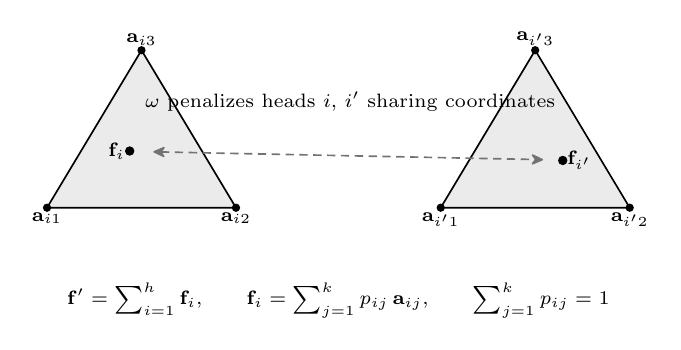
\begin{tikzpicture}[
    font=\footnotesize,
    >={Stealth[round,length=1.8mm,width=1.6mm]},
    lab/.style={inner sep=1.5pt, font=\scriptsize},
  ]
  %% ---- head i --------------------------------------------------------
  \fill[black!8]   (0,0) -- (2.4,0) -- (1.2,2.0) -- cycle;
  \draw[semithick] (0,0) -- (2.4,0) -- (1.2,2.0) -- cycle;
  \fill (0,0)     circle (1.5pt) node[below,lab]{$\mathbf{a}_{i1}$};
  \fill (2.4,0)   circle (1.5pt) node[below,lab]{$\mathbf{a}_{i2}$};
  \fill (1.2,2.0) circle (1.5pt) node[above,lab]{$\mathbf{a}_{i3}$};
  \fill (1.05,0.72) circle (1.7pt) node[left,lab]{$\mathbf{f}_i$};

  %% ---- head i' ------------------------------------------------------
  \fill[black!8]   (5.0,0) -- (7.4,0) -- (6.2,2.0) -- cycle;
  \draw[semithick] (5.0,0) -- (7.4,0) -- (6.2,2.0) -- cycle;
  \fill (5.0,0)   circle (1.5pt) node[below,lab]{$\mathbf{a}_{i'1}$};
  \fill (7.4,0)   circle (1.5pt) node[below,lab]{$\mathbf{a}_{i'2}$};
  \fill (6.2,2.0) circle (1.5pt) node[above,lab]{$\mathbf{a}_{i'3}$};
  \fill (6.55,0.60) circle (1.7pt) node[right,lab]{$\mathbf{f}_{i'}$};

  \draw[<->, densely dashed, semithick, black!55] (1.35,0.71) -- (6.30,0.61);
  \node[lab] at (3.85,1.35)
    {$\omega$ penalizes heads $i$, $i'$ sharing coordinates};

  \node[lab, anchor=north, align=center] at (3.7,-0.9)
  {$\mathbf{f}'=\sum^h_{i=1} \mathbf{f}_i$,\qquad
  $\mathbf{f}_i=\sum^k_{j=1} p_{ij}\,\mathbf{a}_{ij}$,\qquad $\sum^k_{j=1} p_{ij}=1$};
\end{tikzpicture}


\caption[Per-head geometry]{\texttt{DictBlock} \textbf{head geometry} for $h{=}2$, $k{=}3$.
	Each head's output $\mathbf{f}_i$ lies in the simplex spanned by its
	atoms $\mathbf{a}_{ij}$, at the point its assignment picks. The support
	overlap $\omega$ compares heads: driving it to zero would give them
	disjoint coordinates (Section~\ref{sec:disjoint}).}
\label{fig:head-simplex}
\end{figure}

\subsubsection{Decoder}
\label{sec:decoder}
Each $\dictenc$ output $\mathbf{f}'_\ell$, scaled by its input's gain
$g_\ell$, is added to an accumulator $\mathbf{r}$, whose state after
$\ell$ layers is

\begin{equation}
	\mathbf{r}_\ell = \sum_{\ell'=0}^{\ell-1} g_{\ell'}\,\mathbf{f}'_{\ell'},
	\qquad
	g_\ell := \mathrm{sg}\!\left[\mathrm{L2}(\mathbf{y}_\ell)\right]
	\label{eq:accum}
\end{equation}

Under \texttt{resid\_gain} a layer classifies only the direction of its
input, so the gain carries the magnitude it cannot see; without it
$g_\ell = 1$. The empty sum makes $\mathbf{r}_0 = \mathbf{0}$, so layer 0's
input is the encoded input itself, $\mathbf{y}_0 = \mathbf{x}$, whose gain
is identically 1 on unit-norm SONAR embeddings.

A single-layer unbiased linear decoder $\mathrm{dec}$ projects
$\mathbf{r}_\ell$ back to the input space $\mathbb{R}^d$. Weights
$W_{\mathrm{dec}} \in \mathbb{R}^{d \times e}$
are shared for all $\mathtt{DictEnc}_\ell$.

\begin{equation}
	\hat{\mathbf{x}}_\ell = W_{\mathrm{dec}}\,\mathbf{r}_\ell
	\label{eq:dec}
\end{equation}

The residual $\mathbf{y}_\ell$, layer $\ell$'s input, is given by
$\mathbf{x} - \hat{\mathbf{x}}_\ell$, stop-gradiented so that
lower layers cannot write a communication code into the residual instead
of reducing it. Layer $\ell$ splits it into the gain $g_\ell$
(Eq.~\eqref{eq:accum}) and a shape $\mathbf{u}_\ell$, its unit direction
with a constant coordinate appended, which is what the classifier, the
router and the fibers read; $\epsilon$ is the floating-point epsilon of
the working dtype.

\begin{equation}
	\mathbf{y}_\ell = \mathrm{sg}\!\left[\mathbf{x} - \hat{\mathbf{x}}_\ell\right],
	\qquad
	\mathrm{L2}(\mathbf{y}) := \sqrt{\sum^{d}_{q=1} y_q^2}
	\label{eq:L2}
\end{equation}

\begin{equation}
	\mathbf{u}_\ell =
	\frac{\mathbf{y}_\ell}{\mathrm{L2}(\mathbf{y}_\ell) + \epsilon} \oplus [1]
	\label{eq:y_norm}
\end{equation}

Normalizing fixes the classifier's input scale: a bilinear classifier's
logits scale with the square of its input's norm, so they would explode
on large inputs (raw GPT-2 activations) and vanish on the small residuals
deep layers see; the gain carries the magnitude instead. This is the
re-scaling invariance of RMSNorm~\cite{zhang2019rms} without its learned
gain, on the unit sphere rather than RMSNorm's sphere of radius
$\sqrt{d}$, which is why the classifier's initial logits are small
(Appendix~\ref{sec:calib}).
A constant coordinate $[1]$ is appended, giving a dimension of $d+1$.
This prevents the sign information of $\mathbf{y}_\ell$ from being lost
by the bilinear transformation.
Effectively, it adds a bias to an otherwise unbiased linear form
while preserving eigendecomposition. This is the input augmentation by
which Pearce et al.~\cite{pearce2025} give bilinear layers biases; it
splits each output into an interaction, a linear and a constant term.

\subsubsection{Noise}
\label{sec:noise}
Noise is added to $X$, $\mathsf{K}$, and $\mathsf{F}$, controlled by
hyperparameters $\sigma_X$, $\sigma_K$, and $\sigma_F$. Each draws a
standard normal of the same shape as its target,

\begin{equation}
	\varepsilon \sim \mathcal{N}(0,1)
\end{equation}

and scales it three different ways. Classifier logits take unscaled
Gaussian noise,

\begin{equation}
	\mathrm{noise}_{\mathrm{normal}}(\mathsf{K}) :=
	\mathsf{K} + \sigma_K\varepsilon
	\label{eq:noise_normal}
\end{equation}

inputs take noise proportional to their own norm, so the scale is a
fraction of signal magnitude rather than an absolute quantity,

\begin{equation}
	\mathrm{noise}_{\mathrm{batchnorm}}(X) := X + \sigma_X\,\varepsilon
	\odot \frac{\mathrm{sg}\!\left[\mathrm{L2}(X)\right]}{\sqrt{d}}
	\label{eq:noise_batchnorm}
\end{equation}

and features take noise proportional to each feature's standard
deviation across the batch.

\begin{equation}
	\mathrm{noise}_{\mathrm{featvar}}(\mathsf{F}) := \mathsf{F} +
	\sigma_F\,\varepsilon \odot \mathrm{sg}\!\left[
	\sqrt{\mathrm{var}_n(\mathsf{F}) + \epsilon}\right]
	\label{eq:noise_featvar}
\end{equation}

Here $\mathrm{L2}(X)$ is the per-sample norm of
Eq.~\eqref{eq:L2}, broadcast over $d$. Both scales are
stop-gradiented: without $\mathrm{sg}$ the model could evade its own
noise by shrinking feature variance, and the $\epsilon$ inside the root
guards the $0/0$ gradient where a feature's batch variance underflows to
exactly zero. Because $\sigma_K$ enters the softmax as $\sigma_K/t$,
holding it constant under a falling temperature would grow effective
exploration rather than hold it, so models with an annealed temperature
anneal $\sigma_K$ with it. Each model's noise settings are in
Appendix~\ref{app:configs}.

\subsubsection{Router and fibers}
\label{sec:router-fiber}
Two optional branches read the same shape $\mathbf{u}$ as the classifier
(Eq.~\eqref{eq:y_norm}, with the layer index dropped) and meet it in
the dictionary lookup
(Figure~\ref{fig:dictenc-full}). Both are optional; the models that use
them are listed in Appendix~\ref{app:configs}.

The \emph{router} (\texttt{scaled}) is a second bilinear map, from
$\mathbf{u}$ to one scale per head, $\boldsymbol{\gamma} \in \mathbb{R}^h$,
made non-negative by an absolute value
(\texttt{router\_signed} drops it). Its scale $\gamma_i$ multiplies head
$i$'s whole output, so
the classifier decides \emph{what} a head says and the router \emph{how
much}; its own L1, $\mathrm{L1}_S$, prices the router alone, where
$\mathrm{L1}$ on the output can be paid down by either factor.

\emph{Fibers} (\texttt{fiber\_rank} $r$) give every entry a local basis
$U_{ij} \in \mathbb{R}^{e \times r}$ (in its head's slice under
$\mathtt{ConcatDictBlock}$), and each head reads $r$ coordinates
$\mathbf{c}_i = \beta\tanh(A_i\mathbf{u}/\beta)$ from the input, so
\begin{equation}
	\mathbf{f}_i = \gamma_i \sum^{k}_{j=1} p_{ij}\,\big(\mathbf{a}_{ij}
	      + U_{ij}\,\mathbf{c}_i\big).
	\label{eq:fiber}
\end{equation}
Under a hard code the selected entry is a discrete base point and the
fiber a continuous correction within the plane its basis spans
(Figure~\ref{fig:fiber}). Unconstrained, the correction can take over and
leave the base meaningless, so the base is kept honest by fiber dropout, a
norm cap ($\lVert U_{ij}\mathbf{c}_i\rVert \le \rho$ per head, or
summed over heads), a base-only deep-supervision term (\texttt{base\_aux},
which also decodes the fiber-free output), or training the fibers after
freezing the base. A radial fiber ($r{=}1$, no basis) only rescales the
selected entry. Statistics describe the base output. Head dropout
(\texttt{p\_head\_drop}) is the third addition here: in training it
replaces a head's classification by the batch mean, its origin, so heads
cannot co-adapt and ablating one to its origin stays in distribution.

\begin{figure}[tp]
\centering
\resizebox{\linewidth}{!}{% DictEnc with the router (`scaled`) and fibers (`fiber_rank`). Three
% branches read the shaped input u and meet in the dictionary lookup:
% the classifier picks entries (P), the router scales each head (gamma),
% and the fiber read gives each head local coordinates (C). Dashed boxes above
% an arrow act on it in training; dashed boxes below are statistics.
\begin{tikzpicture}[
    font=\footnotesize,
    >={Stealth[round,length=1.8mm,width=1.6mm]},
    blk/.style={draw, rounded corners=2pt, align=center,
                minimum height=8mm, inner xsep=4pt},
    hook/.style={draw, rounded corners=2pt, densely dashed, align=center,
                 inner sep=3pt, font=\scriptsize, black!55},
    mul/.style={draw, circle, minimum size=4.5mm, inner sep=0pt},
    lab/.style={inner sep=1.5pt, font=\scriptsize, align=center},
    sig/.style={->, semithick, align=center},
    aux/.style={->, densely dashed, semithick, black!45},
  ]

  %% ---- gain-shape split ------------------------------------------------
  \node[lab] (E)  at (-1.4,0) {$\mathbf{y}$};
  \node[blk] (GS) at ( 0.6,0) {gain--shape\\
                               $\mathbf{u}=\mathbf{y}/\lVert\mathbf{y}\rVert\oplus 1$};
  \draw[sig] (E) -- (GS);
  \coordinate (B) at (2.3,0);
  \draw[semithick] (GS.east) -- node[above,lab,pos=0.55]{$\mathbf{u}$} (B);
  \fill (B) circle (1.1pt);

  %% ---- three branches from u ---------------------------------------------
  % router: one non-negative scale per head
  \node[blk] (RT) at (4.4, 2.2) {$\bilinear^{d \to h}$\\ router};
  \node[blk] (AB) at (7.4, 2.2) {$\lvert\cdot\rvert$};
  % classifier: which entry, per head
  \node[blk] (CL) at (4.4, 0)   {$\bilinearblock^{d \to h \times k}$\\ classifier};
  \node[blk] (SM) at (7.4, 0)   {$\mathrm{softmax}_k(\cdot/t)$\\ or STE};
  % fiber read: r local coordinates per head
  \node[blk] (FR) at (4.4,-2.2) {$\mathsf{A} \in \mathbb{R}^{h \times r \times d}$\\ fiber read};
  \node[blk] (TB) at (7.4,-2.2) {$\beta\tanh(\cdot/\beta)$};

  \draw[sig] (B) |- (RT.west);
  \draw[sig] (B) -- (CL.west);
  \draw[sig] (B) |- (FR.west);
  \draw[sig] (RT) -- (AB);
  \draw[sig] (CL) -- node[below,lab]{$K$} (SM);
  \draw[sig] (FR) -- (TB);

  %% ---- the lookup ----------------------------------------------------------
  \node[blk, minimum height=5.6cm, text width=3.5cm] (DB) at (11.7,0)
    {$\dictblock$\\[6pt]
     $\mathbf{f}_i = \gamma_i \sum_{j} p_{ij}\,\big(\mathbf{a}_{ij}
            + U_{ij}\,\mathbf{c}_i\big)$\\[6pt]
     {\scriptsize atom $\mathbf{a}_{ij}$, fiber basis
      $U_{ij}\in\mathbb{R}^{e \times r}$}};

  \draw[sig] (AB) -- node[above,lab,pos=0.35]{$\boldsymbol{\gamma}\in\mathbb{R}^{h}$} (AB -| DB.west);
  \draw[sig] (SM) -- node[below,lab,pos=0.3]{$P\in\Delta_k^{h}$} (DB.west |- SM);
  \draw[sig] (TB) -- node[above,lab,pos=0.35]{$C\in\mathbb{R}^{h \times r}$} (TB -| DB.west);

  %% ---- combine heads, restore the gain --------------------------------------
  \node[blk] (CB) at (15.5,0) {$\sum_i$ \ or\ $\bigoplus_i$\\ {\scriptsize (concat)}};
  \node[mul] (MG) at (17.3,0) {$\times$};
  \node[lab] (F)  at (18.6,0) {$g\,\mathbf{f}'$\\ layer\\ output};
  \draw[sig] (DB.east |- CB) -- node[below,lab]{$F$} (CB);
  \draw[sig] (CB) -- node[above,lab]{$\mathbf{f}'$} (MG);
  \draw[sig] (MG) -- (F);
  \draw[sig] (GS.south) -- (0.6,-4.1) -| node[pos=0.25,below,lab]
       {$g=\lVert\mathbf{y}\rVert$, stop-gradient} (MG.south);

  %% ---- training-time hooks and the intervention interface (above) -------------
  \node[hook] (nk) at (5.9, 1.0) {$+\,\varepsilon_K$, winner dropout};
  \draw[aux] (nk) -- (5.9,0.2);
  \node[hook] (hd) at (8.95, 1.0) {head dropout\\ \texttt{DictIntervention}};
  \draw[aux] (hd) -- (8.95,0.2);
  \node[hook] (fd) at (8.95,-3.2) {fiber dropout};
  \draw[aux] (fd) -- (8.95,-2.4);
  \node[hook] (nf) at (15.5, 1.6) {$+\,\varepsilon_F$ on the base;\\
                                   fiber norm cap};
  \draw[aux] (nf) -- (14.05,0.2);

  %% ---- statistics (below) ------------------------------------------------------
  \node[hook] (sp) at (7.4,-1.1)
    {$H$\quad $\mathrm{KL}_m$\quad $\mathrm{cossim}_b$};
  \draw[aux] (SM.south) -- (sp);
  \node[hook] (ss) at (7.4, 3.45) {$\mathrm{L1}_S$};
  \draw[aux] (AB.north) -- (ss);
  \node[hook] (sf) at (11.7,-3.45)
    {$\mathrm{L1}$\quad $\omega$\quad $\kappa_i$\\ (base output and atoms)};
  \draw[aux] (DB.south) -- (sf);
  \node[hook] (ba) at (15.5,-1.9) {fiber-free $\mathbf{f}'_{\mathrm{base}}$\\
                                   (\texttt{base\_aux})};
  \draw[aux] (DB.east |- ba) -- (ba);

\end{tikzpicture}
}
\caption[\texttt{DictEnc} with router and fibers]{\textbf{\texttt{DictEnc}
	with router and fibers.} The gain--shape split hands the unit input
	$\mathbf{u}$ to three branches: the classifier (which entry, $P$),
	the router (how much, $\boldsymbol{\gamma}$, one non-negative scale per
	head) and the fiber read (where within the entry's fiber, $C$, $r$
	coordinates per head). They meet in the lookup
	(Eq.~\eqref{eq:fiber}), and the combined heads are scaled by the
	measured gain $g$. Dashed boxes above an arrow act on it in training;
	dashed boxes below are statistics of the fiber-free base output.}
\label{fig:dictenc-full}
\end{figure}

\begin{figure}[tp]
\centering
% One head's geometry with a fiber, extending tikz/dict.tex: the head
% selects the entry with atom a_{i2}; its fiber is the plane U_{i2} spans at that entry,
% and the coordinates c_i place the output within it. The dashed circle is
% the norm cap (`fiber_eps`); the dotted ray is the radial variant, which
% only rescales the entry. Coordinates are precomputed (no calc library):
% d2 = (3.6, 3.2), basis columns u1 = (0.9, 0.25), u2 = (-0.2, 0.8).
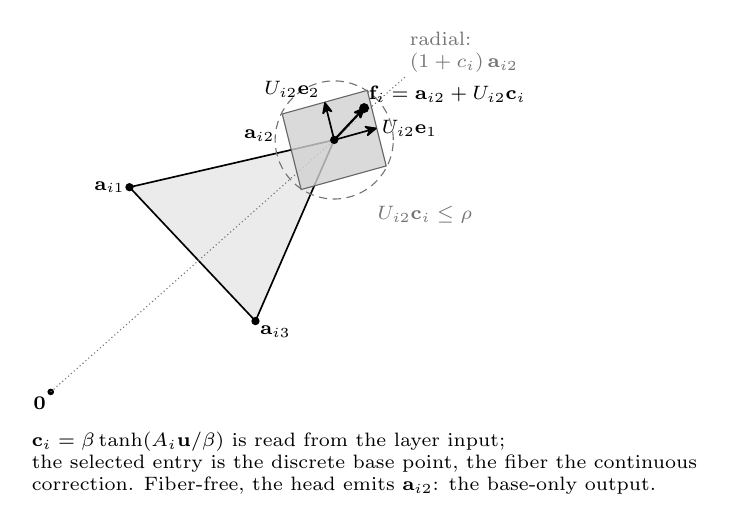
\begin{tikzpicture}[
    font=\footnotesize,
    >={Stealth[round,length=1.8mm,width=1.6mm]},
    lab/.style={inner sep=1.5pt, font=\scriptsize},
  ]
  %% ---- origin and the head's simplex ----------------------------------
  \fill (0,0) circle (1.2pt) node[below left,lab]{$\mathbf{0}$};
  \fill[black!8]   (1.0,2.6) -- (3.6,3.2) -- (2.6,0.9) -- cycle;
  \draw[semithick] (1.0,2.6) -- (3.6,3.2) -- (2.6,0.9) -- cycle;
  \fill (1.0,2.6) circle (1.5pt) node[left,lab]{$\mathbf{a}_{i1}$};
  \fill (2.6,0.9) circle (1.5pt) node[below right,lab]{$\mathbf{a}_{i3}$};

  %% ---- radial variant: a per-entry gain along the entry's own ray ------
  \draw[densely dotted, black!55] (0,0) -- (4.5,4.0)
    node[above right,lab,align=left]{radial:\\ $(1+c_i)\,\mathbf{a}_{i2}$};

  %% ---- the fiber at the selected entry ---------------------------------
  \fill[black!18, opacity=0.8]
    (4.02,3.83) -- (4.26,2.87) -- (3.18,2.57) -- (2.94,3.53) -- cycle;
  \draw[black!60]
    (4.02,3.83) -- (4.26,2.87) -- (3.18,2.57) -- (2.94,3.53) -- cycle;
  \draw[densely dashed, black!55] (3.6,3.2) circle (0.75);
  \node[lab, black!55] at (4.75,2.25) {$\lVert U_{i2}\mathbf{c}_i\rVert \le \rho$};

  \draw[->, semithick] (3.6,3.2) -- (4.14,3.35)
    node[right,lab]{$U_{i2}\mathbf{e}_1$};
  \draw[->, semithick] (3.6,3.2) -- (3.48,3.68)
    node[above left,lab]{$U_{i2}\mathbf{e}_2$};

  \fill (3.6,3.2) circle (1.5pt);
  \node[lab, anchor=east] at (2.9,3.25) {$\mathbf{a}_{i2}$};

  %% ---- the output: base point plus its fiber offset ---------------------
  \draw[->, thick] (3.6,3.2) -- (3.98,3.605);
  \fill (3.98,3.605) circle (1.8pt);
  \node[lab, anchor=south west] at (3.98,3.62)
    {$\mathbf{f}_i = \mathbf{a}_{i2} + U_{i2}\mathbf{c}_i$};

  %% ---- legend ------------------------------------------------------------
  \node[lab, anchor=north west, align=left] at (-0.3,-0.45)
    {$\mathbf{c}_i = \beta\tanh(A_i\mathbf{u}/\beta)$ is read from the layer input;\\
     the selected entry is the discrete base point, the fiber the continuous\\
     correction. Fiber-free, the head emits $\mathbf{a}_{i2}$:
     the base-only output.};
\end{tikzpicture}

\caption[Fiber geometry]{\textbf{Fiber geometry} for one head, extending
	Figure~\ref{fig:head-simplex}. The head selects the entry with atom
	$\mathbf{a}_{i2}$; its fiber is the plane spanned by
	$U_{i2}$ at that point, and the coordinates $\mathbf{c}_i$ place the
	output within it. The dashed circle is the per-head norm cap; the
	dotted ray is the radial variant, which moves the output only along
	the atom's own direction.}
\label{fig:fiber}
\end{figure}

\subsection{Training}
\label{sec:training}

\subsubsection{Embedding model}
\label{sec:sonar}
We embed texts using SONAR~\cite{sonar}, a multimodal and
language-agnostic sentence embedding model: a translation-trained encoder
whose states are mean-pooled into one 1024-dimensional vector, and a
decoder that generates text from that vector alone, in a target language
chosen at decoding time. Each embedding here covers the opening of a web
document (up to its first 512 tokens), longer than the sentences SONAR is
trained on. Translations embed close together, so a reconstructed or
steered embedding can be decoded in one fixed language and re-encoded,
which is how text fidelity and text-cycle steering are scored
(Appendices~\ref{sec:textfid} and~\ref{sec:steertext}).
Large Concept Models~\cite{lcmteam2024largeconceptmodelslanguage}
generate directly in SONAR space, one sentence embedding per step, which
makes it a natural substrate for steering experiments: an edit to a SONAR
embedding is an edit to such a model's context or output. The same work
finds SONAR decoding fragile, with small perturbations of an embedding
able to lose much of its meaning once decoded.

\subsubsection{Loss function}
\label{sec:loss}
Reconstruction fidelity is trained with $\mathrm{MSE}$, where
$\mathbf{w} \in \mathbb{R}^d$ is a fixed per-dimension weight vector.

\begin{equation}
	\mathrm{MSE}(X,\hat{X}) := \frac{1}{bd}\sum^{b}_{n=1}\sum^{d}_{q=1}
	w_q\left(\hat{x}_{nq} - x_{nq}\right)^2
	\label{eq:mse}
\end{equation}

The total objective adds the ghost-gradient reconstruction and the
auxiliary statistics, each weighted by a scalar. Statistics are
\emph{summed} over the $l$ layers rather than averaged.

\begin{equation}
	L := \mathrm{MSE}(X,\hat{X})
	+ s_g\,\mathrm{MSE}(\hat{X}_g,\, X - \hat{X})
	+ \sum^{l-1}_{\ell=0}\mathbf{s}\cdot\boldsymbol{\psi}_\ell
	\label{eq:loss_total}
\end{equation}

Each layer contributes the statistics (Algorithms~\ref{alg:dictblock}
and~\ref{alg:dictenc})

\begin{equation}
	\boldsymbol{\psi}_\ell = \big[\,
	\mathrm{L1}_K \;\; \mathrm{L1} \;\; H \;\; \mathrm{cossim}_b \;\;
	\mathbb{E}_i\kappa_i \;\; \max_i \kappa_i \;\;
	\mathrm{KL}_m \;\; \mathrm{KL}_{\mathrm{pwak}} \;\; \mathrm{L2}_{\mathrm{pwak}}
	\;\; \mathrm{L1}_S \;\; \omega
	\,\big]^{\top}_\ell
	\label{eq:stats}
\end{equation}

where $\mathrm{L1}_K$ is the L1 of the classifier's gate, $\kappa_i$ the
mean within-head cosine between head $i$'s atoms,
$\mathrm{KL}_{\mathrm{pwak}}$ and $\mathrm{L2}_{\mathrm{pwak}}$ the two
partition-consensus statistics, and $\mathrm{L1}_S$ the router's L1. The
max of $\kappa_i$ is logged for a setpoint controller and never itself
penalized. Appendix~\ref{app:stats} gives the implementation's row
layout.

Each model's weights are in Appendix~\ref{app:configs}. The ghost path
is disabled throughout, since $\hat{X}_g$ fires only on features that
are exactly zero across the whole batch, which bilinear classifiers with
softmax selection and absolute-valued dictionaries never produce.

\begin{algorithm}[tp]
	\caption{$\ontologizer$ in training (\texttt{Ontologizer.withStats})
	and the loss it feeds (\texttt{Hyperparams.loss}), for the
	residual forward (\texttt{forward="resid"}) every configuration here
	uses. Without an encoder, $\mathrm{enc}$ is the identity; with direct
	atoms, $\mathrm{dec}$ is.}
	\label{alg:ontologizer}
	\DontPrintSemicolon

	\KwIn{batch $X \in \mathbb{R}^{b \times d}$}
	\KwData{encoder $\mathrm{enc}$; layers $\dictenc_0, \dots, \dictenc_{l-1}$
		(Algorithm~\ref{alg:dictenc}); decoder $\mathrm{dec}$
		(Eq.~\eqref{eq:dec}); MSE weights $\mathbf{w}$; loss weights
		$\mathbf{s}$, $s_g$}
	\Hyper{input noise $\sigma_X$; deep supervision; \texttt{deepsup\_sg};
		\texttt{resid\_norm}, \texttt{resid\_const}, \texttt{resid\_gain}}
	\KwOut{loss $L$; per-layer statistics $\boldsymbol{\psi}_0, \dots,
		\boldsymbol{\psi}_{l-1}$}

	\Begin{
		$E \leftarrow \mathrm{enc}\big(\mathrm{noise}_X(X)\big)$
			\tcp*{Eq.~\eqref{eq:noise_batchnorm}}
		$R \leftarrow \mathbf{0} \in \mathbb{R}^{b \times e}$
			\tcp*{state 0: no layers applied}
		$E \leftarrow E \oplus [1]$ \tcp*{if \texttt{resid\_const}}
		\For(\tcp*[f]{layer $\ell$ reads state $\ell$, writes state $\ell+1$}){$\ell \leftarrow 0$ \KwTo $l-1$}{
			$R_{\mathrm{prev}} \leftarrow R$\;
			$R, \mathsf{P}_\ell, \boldsymbol{\psi}_\ell \leftarrow \dictenc_\ell(R, E)$\;
			\If(\tcp*[f]{a decode per prefix}){deep supervision}{
				$\hat{X}_{\ell+1} \leftarrow \mathrm{dec}\big(R - R_{\mathrm{prev}}
					+ \mathrm{sg}[R_{\mathrm{prev}}]\big)$
					\tcp*{$\mathrm{dec}(R)$ without \texttt{deepsup\_sg}}
			}
			\If{$\ell < l-1$}{
				$Y \leftarrow \mathrm{sg}\big[X - \mathrm{dec}(R)\big]$
					\tcp*{Eq.~\eqref{eq:L2}}
				$E \leftarrow Y \oplus [1]$
					\tcp*{if \texttt{resid\_const}; the next layer splits it
					into gain and shape, Eq.~\eqref{eq:y_norm} (normalized here
					instead under \texttt{resid\_norm} alone)}
			}
		}
		\lIf{not deep supervision}{$\hat{X}_{l} \leftarrow \mathrm{dec}(R)$}
		$\mathrm{MSE} \leftarrow \mathbb{E}_\ell\,
			\mathrm{MSE}_{\mathbf{w}}(X, \hat{X}_\ell)$
			\tcp*{Eq.~\eqref{eq:mse}; over the prefixes computed, each weighted $1/l$}
		$L \leftarrow \mathrm{MSE} + s_g\,\mathrm{MSE}_g
			+ \mathbf{s} \cdot \sum_{\ell=0}^{l-1} \boldsymbol{\psi}_\ell$
			\tcp*{Eq.~\eqref{eq:loss_total}; $\mathrm{MSE}_g = 0$ without
			ghosts}
		\Return{$L$, $(\boldsymbol{\psi}_\ell)_{\ell=0}^{l-1}$}\;
	}
\end{algorithm}


Reconstruction is trained with deep supervision~\cite{lee2015deeply}:
$\mathrm{MSE}(X, \mathrm{dec}(R_\ell))$ is computed separately for
every prefix $\ell = 1, \dots, l$ and averaged, so each prefix carries
weight $1/l$ and each
layer must explain what previous layers left
unexplained. Supervising every prefix through one shared decoder is the
deterministic counterpart of SoundStream's quantizer dropout, which trains
a residual quantizer at a random depth per example~\cite{zeghidour2021},
and the nested-prefix loss of Matryoshka SAEs~\cite{bussmann2025} applied
to a residual stack rather than to prefixes of one dictionary.
A stop-gradient variant (\texttt{deepsup\_sg}, off in every
reported model) stops each prefix's gradient at the accumulator it was
handed, so that a layer trains only against its own residual. The MSE is whitened: $\mathbf{w}$ in
Eq.~\eqref{eq:mse} is the per-dimension inverse variance, normalized
to mean one, the same whitening the evaluation applies. The
implementation applies $\sqrt{\mathbf{w}}$ to $X$ and
$\mathrm{dec}(R_\ell)$ before the squared error, which is equivalent.
Four statistics are active as loss terms in the reported models
(Figure~\ref{fig:dictenc}; Appendix~\ref{app:configs}):
between-sample similarity $\mathrm{cossim}_b$, computed from $P$
through the dictionary Gram so it measures feature-space similarity of
the per-head reconstructions, and which in practice also minimizes
per-sample entropy $H$; the batch-mean term $\mathrm{KL}_m$, anchoring
each head's mean
assignment vector to a uniform distribution so that a uniform code
corresponds to a maximally generic feature; an $\mathrm{L1}$ penalty on
features; and a between-head disjointness term, the support overlap
$\omega$, which measures the extent to which heads use nonoverlapping
coordinates of the dictionary space. Most reported models trained before
$\omega$ existed and used its predecessor (Appendix~\ref{app:stats}).
$\mathrm{L1}$ tends to fall under MSE alone; including it in the loss
speeds up convergence. Classification sharpness is controlled by the
temperature. Winner dropout and the noise terms
$\varepsilon_K$ and $\varepsilon_F$ regularize classifications and
features respectively.

\subsection{Evaluation}
Evaluation runs against $\topk$ SAEs trained on identical cached SONAR
embeddings under an identical whitened reconstruction objective. The
battery follows SAEBench~\cite{karvonen2025} in judging a dictionary
with many instruments rather than by reconstruction at fixed sparsity,
and adapts three of its eight metrics: a loss-recovered analogue, as
downstream text fidelity through the paired M2M100 decoder; blinded
autointerp detection scoring; and sparse probing, of language. The rest
is specific to this comparison: a reconstruction-versus-capacity Pareto;
categorical-form and semantic-coherence tests of head structure;
cross-model feature splitting and seed stability; shrinkage
decomposition; and steering fidelity. A
structural-ablation ladder of SAE variants, each adding one
Ontologizer-style commitment at a time, attributes effects to specific
structure. AxBench~\cite{wu2025axbenchsteeringllmssimple} found that
prompting, finetuning and one simple supervised direction, the
difference of means, beat SAE latents at steering, while a linear
probe's direction did not; the steering comparison here, which includes
both, is built to face that result.




\subsection{Data, models and evaluation}
\label{sec:setup}

This section is an overview; Appendix~\ref{app:methods} is the full
description, with every evaluation's defining equation or algorithm.

\paragraph{Data.}
The SONAR models train on a fixed cache of 4{,}000{,}000 unit-norm SONAR
sentence embeddings ($d{=}1024$) from an interleaved 86-language mC4
sample, with a language label per row and text recoverable by row index;
80 of the 86 languages, 93\% of rows, were encoded under SONAR's English
source tag rather than their own, and a companion sentence-split cache
(\texttt{mc4\_sent16}, 44.1M consecutive segments) stores unnormalized
embeddings under native tags (Appendix~\ref{app:data}).
Sections~\ref{sec:gpt2} and~\ref{sec:seeds} also use residual-stream
activations of GPT-2 small~\cite{radford2019} at the output of block 8 of
12 ($d{=}768$), a substrate where sparse dictionary learning is known to
work~\cite{gao2024}; Section~\ref{sec:gpt2hard}'s
separate GPT-2 setup compares only within that section
(Appendix~\ref{app:data}).

\paragraph{Objective and score.}
Every model minimizes the whitened MSE of Eq.~\eqref{eq:mse}, and we
report whitened FVU (Eq.~\eqref{eq:fvu}) on the final 32{,}768 cache
rows, which SAEs and straight-through arms never train on (coordinate~837,
fixed on raw SONAR embeddings by the final LayerNorm hyperplane, reads out
$1/\lVert\mathbf{x}^{\mathrm{raw}}\rVert$ after L2 normalization and holds
at most $0.41\%$ of any sparse model's whitened error;
Appendix~\ref{app:data}). The softmax
Ontologizers predate that holdout, but their scores move by at most
0.3\% on freshly encoded rows that no model saw
(Appendix~\ref{app:data}). Every score uses the run's own final
temperature.

\paragraph{Models.}
The reference softmax Ontologizer \texttt{resid\_nc} has $l{=}5$ residual
layers of $h{=}32$ heads with $k{=}32$ entries; a selection sweep varies
only its selection rule, and the straight-through arm
(Section~\ref{sec:ste}) replaces it with hard codes. The SAEs are $\topk$
SAEs after Gao et al.~\cite{gao2024}, plus a structural-ablation ladder
that adds one Ontologizer constraint at a time. Two of its rungs,
\texttt{g160top1} and \texttt{g160softmax} (160 heads of hard or softmax
competition over a shared decoder), are each a one-layer Ontologizer
without the bilinear classifier, residual stack or non-negative
dictionary, \texttt{g160top1} with a router fused into its classifier,
and are treated as simplified variants rather than baselines
(Appendix~\ref{sec:models}; configurations in Appendix~\ref{app:configs}).

\paragraph{Evaluations.}
Each is a standalone script on the shared eval split
(Appendix~\ref{app:protocols}): reconstruction against code capacity and
a Gaussian rate--distortion reference (\texttt{pareto.py}); whether SAE latents form
exhaustive, exclusive head-like groups (\texttt{headstruct.py}); the
semantic coherence of a head's atoms against size-matched nulls
(\texttt{headcoh.py}); feature splitting and cross-seed head matching by
partition and by contribution (\texttt{splitting.py}, \texttt{partition.py},
\texttt{headcontrib.py}); text fidelity through the M2M100 decoder
(\texttt{textfid.py}); language probing by latent and by partition
(\texttt{langprobe.py}, \texttt{headlang.py}); shrinkage by least-squares
refitting on a frozen support (\texttt{refit.py}); steering fidelity in
text and in embedding space (\texttt{steerfid.py}, \texttt{steerembed.py},
\texttt{steergeom.py}); additivity of paired interventions
(\texttt{compose.py}); and autointerp (\texttt{autointerp.py}).

\section{Results: the softmax Ontologizer against SAEs}
\label{sec:results}

\subsection{The price of structure: reconstruction--capacity Pareto}
\label{sec:pareto}

\begin{figure}[tp]\centering
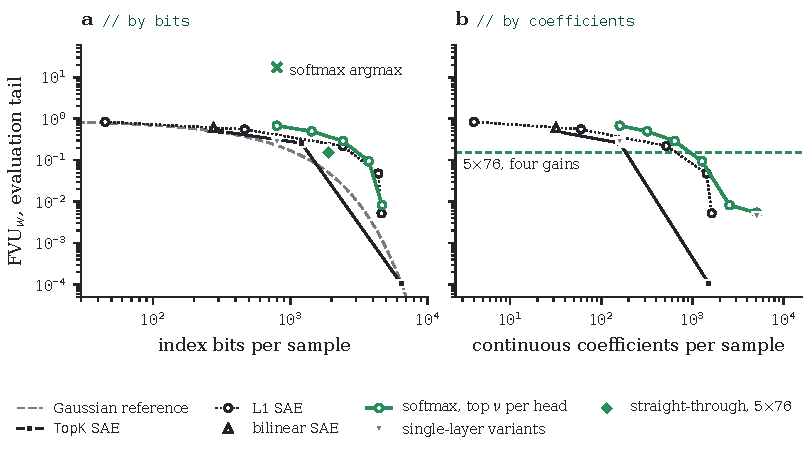
\includegraphics[width=\linewidth]{figures/fig-pareto.pdf}
\caption[Reconstruction against code size]{Reconstruction against code
size on the shared evaluation tail, by index bits (a) and by continuous
coefficients (b): the reference softmax model's truncated codes
(\texttt{resid\_nc}), the SAEs (the L1 SAEs at all five weights of
Table~\ref{tab:cfg-sae}), the single-layer variants and the
straight-through stack (\texttt{ste\_h76\_init01},
Section~\ref{sec:ste}). A code
appears only where its size is nonzero, so the soft codes are in (b)
alone, the softmax argmax is in (a) alone, and the straight-through stack,
whose only continuous numbers are four per-layer gains, is a level in
(b). The dashed curve is the Gaussian reference
(Eq.~\eqref{eq:ratefloor}). Index bits are the whole rate of a hard code,
apart from those gains, but only the support of a code that also sends
coefficients, which is how the $k_{\mathrm{SAE}}{=}32$ and
$k_{\mathrm{SAE}}{=}5120$ SAEs reach the reference in (a);
Figure~\ref{fig:quantrate} puts every code on one rate axis. The softmax
model saw the tail in training and the others hold it out; on rows no
model saw, every point moves by at most 0.3\%, and the dense control's
$1.1\times10^{-4}$ by 0.9\% (Appendix~\ref{app:data}).
One seed per point, except the
$k_{\mathrm{SAE}}{=}32$ SAE's seed-43 replica.}
\label{fig:pareto}
\end{figure}

The SAE frontier dominates the soft Ontologizer's code at every capacity
measured (Figure~\ref{fig:pareto}b). Truncating the reference model's code to the $\nu$ largest
deviations per head from its mean assignment (Appendix~\ref{app:protocols}),
it needs 320 coefficients to reach the $\fvu \approx 0.49$ that the
$k_{\mathrm{SAE}}{=}32$ SAEs reach with 32, and its coarsest code, one
deviation per head (160 coefficients, $\fvu$ 0.677), is already worse than
the SAE's 32-coefficient point, so the very sparse regime is closed to
it. Unstructured reconstruction is better still: the dense control reaches
$\fvu$ $1.1\times10^{-4}$ with $3.4\times$ fewer active coefficients than
the soft code, about $50\times$ lower error at a matched budget. The
truncations are applied after the fact to a model never trained to
truncate, so they may overstate what the structure itself costs: a
residual quantizer degrades when truncated without training for it, and
one trained at a random depth per example does not~\cite{zeghidour2021}. The
code's information is spread across heads: keeping whole heads instead of
deviations is far weaker at matched coefficients ($\fvu$ 0.50 for 8 of 32
heads per layer, against 0.094 at $\nu{=}8$).

The soft model's own discrete reading is not a code. Its argmax
reconstructs at $\fvu$ 17.3, $77\times$ the Gaussian reference for 800
bits (0.226; Figure~\ref{fig:pareto}a), the least distortion an 800-bit code could reach if the
embeddings were Gaussian with their measured covariance
(Eq.~\eqref{eq:ratefloor}). Real embeddings are no harder to compress
than that~\cite[Problem~10.8]{cover2006}, so the argmax sits at least
$77\times$ above the data's distortion--rate function, and on a
selection-sweep run of the same shape the gap is nine orders of magnitude
($8.7\times10^6$ against 0.0007 for the soft code). The entries that
interventions on a softmax model act on are therefore not what carries
its embedding --- the failure VQ-VAE reports for a soft relaxation of
quantization trained from scratch, whose decoder learns to invert the
relaxation~\cite{vandenoord2017} --- which motivates the straight-through
arm of Section~\ref{sec:ste}. The reference does not say that 800 bits are too
few, since non-Gaussian data can be compressed below it.

\subsection{Structure decomposition (the ladder)}

\begin{table}[htbp]\centering\small
\begin{tabular}{@{}lrrl@{}}
\toprule
rung & $\fvu$ & $\mathrm{L0}$ & note \\
\midrule
k32 baseline    & 0.499 & 32   & 0 dead \\
g160top1        & 0.274 & 160  & 1469/5120 dead (29\%) \\
g160softmax     & \textbf{0.0044} & 5120 & beats \texttt{resid\_nc} (0.0054) \\
k32\_p5         & 0.509 & 32   & nested prefixes, $\sim$2\% cost \\
k32\_bl         & 0.602 & 32   & 1920/5120 dead (38\%) \\
\bottomrule
\end{tabular}
\caption{Converged structural rungs, $m{=}5120$, 144.3k steps each.}
\end{table}

Per-head competition sets most of the gap to unstructured codes: the
single-layer soft variant costs about $30\times$ the dense control
($0.0044$ against $1.1\times10^{-4}$). Everything the reference
Ontologizer adds to it (bilinear classifiers, five residual layers, a
shared 2048-dimensional dictionary space) adds nothing to reconstruction,
at $2.2\times$ the parameters. A selection-sweep run of the same shape
does reach 0.0007, six times below the single-layer variant, and keeps
that on rows no model trained on (0.00067 against 0.0044;
Appendix~\ref{app:data}). A stack can therefore beat the single layer out
of sample, but the reference checkpoint does not, so for the model the
rest of this section studies the case has to rest on steering.

Hard per-head selection with a router fused into the classifier
(Appendix~\ref{sec:models}) costs only about 6\% over an unstructured code
of equal sparsity (0.274 for the single-layer hard variant against 0.258
for the $k_{\mathrm{SAE}}{=}160$ SAE). The softmax model's catastrophic
argmax is a training artifact, not a property of discrete head codes:
one-hot selection inflates its output norm $3.7\times$, because winning
atoms carry about $4\times$ the soft mixture's norm, while a stack trained
under the argmax, with no per-head scales at all, reaches $\fvu$ 0.154
(Section~\ref{sec:ste}). A bilinear encoder
costs about 20\% in $\fvu$ and leaves over a third of the dictionary
dead, though its factors start random where every linear rung starts
tied to its decoder (Appendix~\ref{app:configs}), so the cost is not yet
the bilinear form's alone.

Categorical structure appears where it is trained in as hard selection.
The hard variant's partition is head-like, while soft per-head codes
converge to dense, near-uniform mixtures and the SAE's spontaneous groups
are co-firing topical clusters (Appendix~\ref{sec:categorical}). The rest
of the softmax-versus-SAE battery (feature reliability, text fidelity,
language localization and shrinkage) is in Appendix~\ref{app:soft}.

\subsection{Semantic coherence: heads are contrast sets}
\label{sec:prelim-orth}

\begin{figure}[tp]\centering
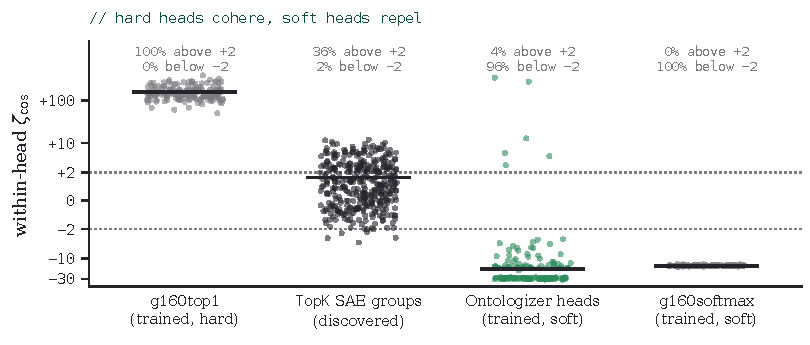
\includegraphics[width=\linewidth]{figures/fig-headcoh.pdf}
\caption[Within-head coherence by head]{Within-head decode-direction
coherence: each head's, or discovered group's, $\zeta_{\cos}$ against a
size-matched null drawn from the same pool ($n_{\mathrm{null}}{=}500$),
on a scale linear between the dotted lines at $\pm2$ and logarithmic
beyond them; bars are means. The
soft heads are those of \texttt{resid\_nc} and \texttt{g160softmax}, the
discovered groups those of the $m{=}11264$, $k_{\mathrm{SAE}}{=}32$ SAE.
One seed per model.}
\label{fig:headcoh}
\end{figure}

Hard-trained heads are coherent, and soft-trained heads are contrast sets
(Figure~\ref{fig:headcoh}).
Every head of the single-layer hard variant decodes to directions far more
similar than a random set of the same size: winner-take-all with a free
magnitude leaves each head one direction at a time, the regime in which
covering a multi-dimensional feature takes many near-collinear
atoms~\cite{dalili2026}, so each head's atoms tile one
region~\cite{bhalla2026manifolds,fel2026structuring}. An SAE's post hoc
co-firing groups are mildly coherent, as topical clusters would be. Both
soft architectures show the opposite: in 96--100\% of heads, the entries'
decode directions are more dissimilar than random sets. Softmax
competition pushes a head's atoms apart, so its entries are
well-separated alternatives, and swapping one for another is a large,
clean move along the head's own dimension. The repulsion does not depend
on the inner product: under the whitened metric the objective optimizes,
it strengthens for the Ontologizer (mean $\zeta_{\cos}$ $-24.4$ against
$-17.6$) and is essentially unchanged for the single-layer variants
(Appendix~\ref{sec:coherence}).

The hard-code Ontologizer shows the same in its weights. Its within-head
atom cosine, decoded into output space, is 0.023 at layer 0 and $-0.015$
to $-0.020$ at layers 1--4, so a head's decoded atoms are orthogonal and
slightly repelling; read in the dictionary space instead, the statistic is
dominated by the decoder's null space (Appendix~\ref{sec:rowcos}). Of the
two orthogonalities in Section~\ref{sec:disjoint}, the within-head one
holds in both code types and the between-head one holds in neither: no
trained model partitions its dictionary space between heads. The support
overlap $\omega$ sits at or above a null that shuffles each head's
coordinates, and each head's usage covers 52--98\% of the coordinates,
where a partition into 32 heads needs about 3\%
(Appendix~\ref{sec:support}). Heads are contrast sets that share their
coordinates.

\subsection{Steering fidelity}
\label{sec:steer}

Steering is measured in embedding space: a step from the input along a
direction, scored by whether the target entry becomes selected (its
realization) and by how many other heads change (its collateral, a side
effect inside the code rather than in the downstream features that SAE
steering studies count~\cite{duan2026}; Algorithm~\ref{alg:steerembed}).
The text round trip cannot resolve an
intervention, because even an unsteered round trip preserves a head's
argmax on only 11--13\% of rows (Appendix~\ref{sec:steertext}).

\begin{table}[htbp]\centering\small
\begin{tabular}{@{}lrr@{}}
\toprule
direction & hard code @0.25 / 1.0 & softmax @0.25 / 1.0 \\
\midrule
decode                       & 0.364 / 0.607 & \textbf{0.824} / 0.569 \\
grad                         & 0.304 / 0.103 & 0.453 / 0.477 \\
margin                       & 0.158 / 0.275 & --- \\
adjoint, oriented            & 0.001 / 0.001 & 0.427 / 0.501 \\
adjoint, oriented per sample & ---           & 0.446 / 0.512 \\
random                       & 0.018 / 0.024 & 0.020 / 0.037 \\
\midrule
collateral                   & 0.66 / 0.88   & 0.58 / --- \\
\bottomrule
\end{tabular}
\caption{Realization rate (target entry newly selected) by direction and
strength; 60--64 entries $\times$ 32 held-out rows, chance 0.031.
Collateral agrees within 0.01 across directions at a given strength, so
rows compare at an equal budget. Hard code: the $5\times76$ stack, whose
seed-43 twin agrees within 0.015 in every decode, grad and random
condition. The adjoint direction's orientation is in
Appendix~\ref{sec:eigorient}.}
\label{tab:steerembed}
\end{table}

In embedding space steering works. The decode direction realizes the
target entry on 82\% of rows for the softmax model at strength 0.25. The
hard code is the less steerable of the two: it realizes 36\% while
already disturbing more of the other heads (0.66 against 0.58), because a
hard argmax has margins a small step cannot cross. Swept over strength,
its decode direction saturates near 0.65 (Figure~\ref{fig:steer-curves}b), so a third of its interventions
cannot be realized at any strength, and it passes the soft model only
beyond collateral 0.85, where most of the other heads have moved too.
Steering by target layer reverses the aggregate ranking of the decode and
gradient directions (Appendix~\ref{sec:steerlayer}). In both stacks the
decode step realizes through directions the data barely vary along: at
the full step's length, its component in the subspace holding the bottom
fifth of the data's variance realizes 95\% (hard) and 100\% (softmax) of
what the whole step does, and its component in the top half 20\% and 8\%
(Appendix~\ref{sec:steernull}).

\paragraph{Against supervised steering vectors.} The same measurement
scores the two standard supervised steering vectors for each target: the
difference of means between rows that select the target and rows that do
not (the mean-difference vector of contrastive activation
addition~\cite{rimsky2024}, which averages over many contrast pairs the
single-pair difference of activation addition~\cite{turner2024}), and the
weight vector of a class-balanced logistic probe, both standard supervised
baselines~\cite{wu2025axbenchsteeringllmssimple}, fitted on 8{,}192
reference rows with the steered rows held out. Unlike contrastive
activation addition's pairs, which differ only in the property, these rows
are unpaired, so the difference also carries whatever else varies with
the target. Their labels are the
code's own selections, so they are an oracle baseline: how well a
supervised method that already knew the partition would steer into it.

\begin{table}[htbp]\centering\small
\begin{tabular}{@{}lrrrr@{}}
\toprule
model & own decode & diff.\ of means & probe & random \\
\midrule
softmax stack & \textbf{0.75} / 0.57 & 0.46 / 0.46 & 0.47 / 0.51 & 0.02 / 0.56 \\
hard-code stack & 0.37 / 0.66 & \textbf{0.91} / 0.63 & \textbf{0.94} / 0.64 & 0.02 / 0.65 \\
hard-code flat & 1.00 / 0.33 & 0.97 / 0.27 & 1.00 / 0.31 & 0.01 / 0.37 \\
untrained stack & 0.02 / 0.22 & 0.75 / 0.22 & \textbf{0.94} / 0.22 & 0.01 / 0.22 \\
random-projection heads & 0.78 / 0.31 & 0.87 / 0.30 & \textbf{1.00} / 0.31 & 0.02 / 0.32 \\
\texttt{g160top1} & 0.58 / \textbf{0.03} & 0.94 / 0.13 & 0.95 / 0.14 & 0.04 / 0.23 \\
\texttt{g160softmax} & 1.00 / 0.30 & 0.99 / 0.27 & 1.00 / 0.31 & 0.01 / 0.34 \\
$\topk$ SAE, $k_{\mathrm{SAE}}{=}32$ ($m{=}11264$) & 1.00 / 0.21 & 0.92 / 0.21 & 0.97 / 0.23 & 0.00 / 0.25 \\
SAE, bilinear encoder & 1.00 / 0.07 & 0.97 / 0.12 & 0.99 / 0.11 & 0.01 / 0.13 \\
\bottomrule
\end{tabular}
\caption{Each model's own steering direction against supervised vectors
fitted to the same targets (realized / collateral), at a step of
$0.25\lVert \mathbf{x}\rVert$; 60--64 targets $\times$ 32 held-out rows per
model, one seed. Untrained stack: the $5\times76$ hard-code stack at step~0
under the fixed initialization. Random-projection heads: $1\times380$
locality-sensitive hash heads of $k{=}32$ bins (\texttt{steerembed.py
--model lsh}), whose ``own decode'' swaps empirical cell centroids
($\mathbf{c}_{ij'} - \mathbf{c}_{ij}$); stepping along the target bin's
projection direction or margin gradient realizes $1.00$ at $0.32$
collateral. An SAE's collateral counts its other active latents, so compare
within a row.}
\label{tab:steersup}
\end{table}

\begin{figure}[tp]\centering
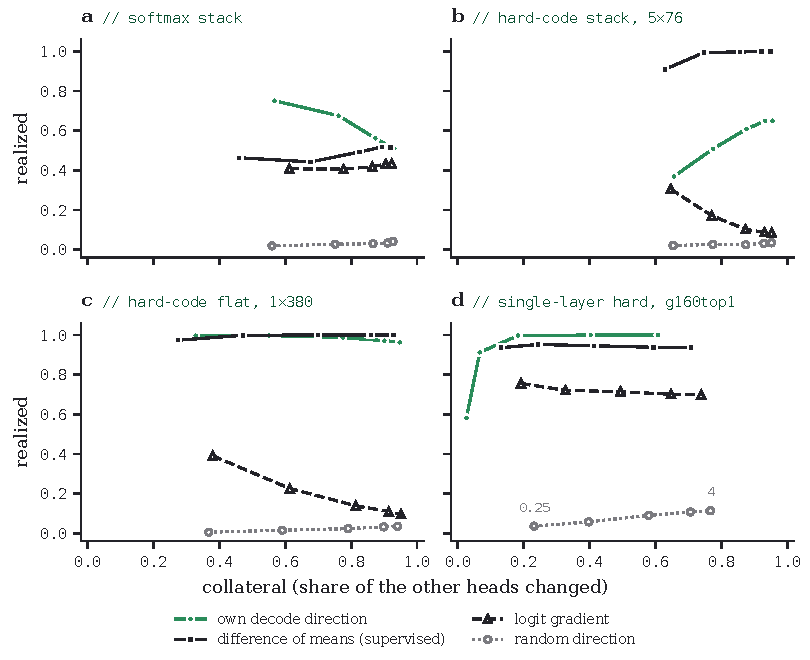
\includegraphics[width=\linewidth]{figures/fig-steer-curves.pdf}
\caption[Steering against collateral by step strength]{Realization
against collateral as the step grows from $0.25\lVert\mathbf{x}\rVert$ to
$4\lVert\mathbf{x}\rVert$, left to right along each curve, on the draw of
Table~\ref{tab:steersup}. (a) The softmax stack
(\texttt{sweep\_softmax\_shm}). (b) The hard-code stack
(\texttt{ste\_h76\_init01}). (c) The flat hard code
(\texttt{ste\_l1\_h380\_i01\_hm1e4}). (d) The single-layer hard variant
\texttt{g160top1}. At each strength the models' own directions disturb
as many other heads as the random step (a direction drawn isotropically
in the embedding's raw coordinates), to within about 0.05, except
\texttt{g160top1}'s decode direction, which disturbs far fewer; what a
direction buys is its height above the random curve. Against a random
step shaped like the data, the softmax stack's own directions disturb
0.14--0.20 more heads at strength 0.25 and the hard codes' at most 0.07
more (Appendix~\ref{sec:steernull}). The logistic probe
tracks the difference of means (within 0.03 realized, 0.05 collateral)
and is not drawn.}
\label{fig:steer-curves}
\end{figure}

Only the softmax stack's own direction beats the supervised vectors,
reaching its categories on 75\% of rows against 46--47\%. The hard-code
stack's categories are reachable, but its own direction misses them: the
supervised vectors reach the same entries on 91--94\% of rows, where its
decode direction reaches 37\%. The single-layer hard variant trades reach
for precision (58\% realized against 94\%, at a fifth of the collateral);
every other model's own direction disturbs the other heads as much as a
random step does. Knowing the partition buys the supervised vectors
little precision (the difference of means sits at most 0.1 below random's
collateral), and an SAE's decoder direction is already as good as the
oracle. Crucially, the two arbitrary-partition rows show that reaching a
partition's cells in embedding space is a property of partitioning the
space, not evidence that the learned partitions are meaningful. In an
untrained $5\times76$ stack, the parametric decode step uses random
dictionary and decoder weights and stays at chance ($0.02$), but the
supervised vectors ($0.75$ and $0.94$) and the classifier's own geometry
(\texttt{grad} $0.61$, \texttt{margin} $0.85$ vs.\ $0.30$ and $0.16$ after
training) reach its random partitions easily and at a third of the trained
stack's collateral ($0.22$ vs.\ $0.66$): training aligns the parametric
decode step with the classifier's cells while moving the stack's heads
closer to their boundaries and tripling collateral. And in $1\times380$
random-projection heads, empirical cell-centroid swaps realize $0.78$ at
strength $0.25$ ($0.67$ at native step) with $0.31$ collateral, while the
target projection vector, margin gradient, and logistic probe each realize
$1.00$ ($0.87$ for difference of means), matching the trained flat arm and
beating the trained hard stack on both reach and collateral. At each
method's own step size the difference of means realizes
more in most models, partly by taking longer steps
(Appendix~\ref{sec:steersupnative}). This tests reaching the model's own
categories; Appendix~\ref{sec:steeroverlay} steers toward an external
concept, language, against supervised vectors fitted to its labels.

A single entry can still steer content: on the reference softmax model,
forcing entry 17 of head 8 in layer 1 reliably yields Burmese decodes of
otherwise preserved content.

\subsection{Description specificity (autointerp)}
\label{sec:autointerp}

Individual SAE latents are about twice as describable as individual
entries. Under the same plain summarization prompt, 51\% of
$k_{\mathrm{SAE}}{=}32$ latents receive a specific description (20\%
naming a language or script), against 23\% of the reference model's
entries (8\%). Blinded detection over the full campaign agrees:

\begin{table}[htbp]\centering\small
\begin{tabular}{@{}lrrrrrrr@{}}
\toprule
model & density & freq & \texttt{params} & \texttt{eig} & \texttt{acts} & \texttt{cacts} & features \\
\midrule
onto (resid\_nc)   & 100\%  & 10.80\% & 0.039 & ---   & 0.473 & 0.392 & 225 \\
k32                & 0.6\%  & 0.61\%  & 0.139 & ---   & 0.645 & 0.603 & 250 \\
k32\_bl            & 0.6\%  & 2.62\%  & 0.136 & 0.034 & 0.578 & 0.470 & 75 \\
g160top1           & 3.1\%  & 5.08\%  & 0.111 & ---   & 0.646 & 0.594 & 150 \\
g160softmax        & 100\%  & 0.00\%  & 0.086 & ---   & 0.449 & 0.364 & 256 \\
k5120 (dense ctrl) & 45.5\% & 17.97\% & 0.010 & ---   & 0.470 & 0.332 & 256 \\
\bottomrule
\end{tabular}
\caption{Mean per-feature detection F1 by description mode
(Appendix~\ref{app:protocols}). The always-match null is about 0.67, and a
generic description that matches every item scores the null, so generic
descriptions inflate toward it. Density is nominal code density; freq is
the firing rate at the $2/k$ threshold. \texttt{k32\_bl}'s pool is only 75
live features; no null control was recorded for this campaign.}
\label{tab:autointerp}
\end{table}

\begin{figure}[tp]\centering
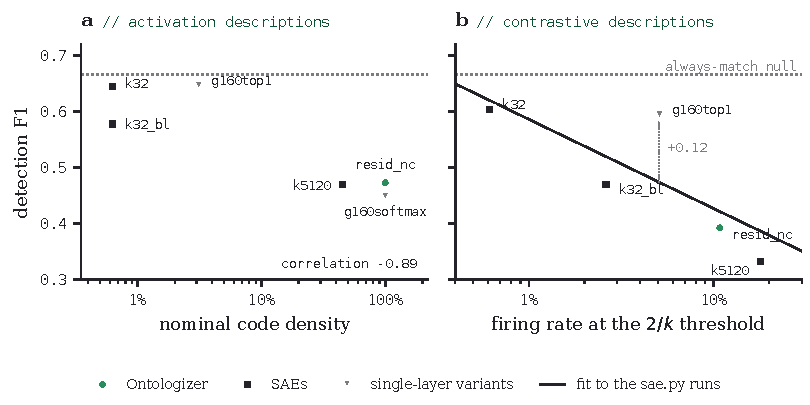
\includegraphics[width=\linewidth]{figures/fig-autointerp-density.pdf}
\caption[Describability against code density]{Mean detection F1 per run
of Table~\ref{tab:autointerp} against code density. (a) Activation
descriptions against nominal density, the share of a code's coefficients
that are nonzero. (b) Contrastive descriptions against the firing rate at
the $2/k$ threshold, with a line fitted in log rate to the four
\texttt{sae.py} runs that fire; \texttt{g160softmax} never crosses the
threshold and is not drawn, and the Ontologizer (\texttt{resid\_nc}) is
held out of the fit. Detection sets are half positives, so a description
that matches every item scores the always-match null, $2/3$ (dotted).
One seed per run.}
\label{fig:autointerp-density}
\end{figure}

Describability tracks code density, not architecture, among the learned
dictionaries compared here (raw model units score lower at similar
sparsity~\cite{paulo2025}). Activation-based
descriptions rank the sparse codes (the $k_{\mathrm{SAE}}{=}32$ SAE and the
single-layer hard variant, 0.65) above the bilinear SAE (0.58), the
reference model and the dense control (0.47) and the single-layer soft
variant (0.45), and density alone carries about 80\% of that variance
(Figure~\ref{fig:autointerp-density}a). Much of it is language. mC4
cycles through 86 languages, and neither the contrastive background nor
the detection negatives are matched for language, so a latent whose top
rows share one is described by naming it and detected against random
rows: 63 of the $k_{\mathrm{SAE}}{=}32$ SAE's 250 latents and 41 of the
hard variant's 150 have their 15 judged rows in one to three languages
and are detected at F1 0.90--0.97, while no dense code has such a latent.
Across the six runs mean language purity accounts for 93\% of the
variance in mean F1 (98\% for contrastive descriptions), though over six
runs it moves with density. Restricted to features whose top rows span
13--15 languages, as random rows do, the gap to the reference Ontologizer
in activation descriptions shrinks from 0.17 to 0.10 for the
$k_{\mathrm{SAE}}{=}32$ SAE and to 0.01 for the hard variant. The reference Ontologizer sits on the SAEs' density
trend, and the hard variant, 0.12 above it on all features
(Figure~\ref{fig:autointerp-density}b), is 0.02 above a trend refitted on
the multilingual ones (Appendix~\ref{sec:headautointerp}). Per-latent
detection F1 therefore cannot compare architectures at unmatched density
or language spread, and every soft Ontologizer is dense by construction.
Distribution-based monosemanticity
scores show the same confound, rising as an SAE's L0 falls at fixed
width~\cite{fereidouni2025evaluatingsparseautoencodersmonosemantic}. The contrastive descriptions
(\texttt{cacts}) give the more honest number, though their background is
not matched for language either: they score below plain summaries
everywhere, least for the sparse codes (by 0.04--0.05) and most for the
dense control (by 0.14), so part of every plain-summary score is generic
matching.

Parameter-space decodes are not descriptions. Decoding the parameters
scores 0.14 at best (the plain and bilinear SAEs) and 0.04 for the
reference model, where activation descriptions of the same features
score 0.45--0.65. Bilinear eigenfeature decodes score 0.034, but they
decode the top-$|\lambda|$ eigenvector, which for most of the bilinear
SAE's latents is a direction the latent rejects (Appendix~\ref{sec:models}),
so that score does not test eigenfeatures. Part of the parameter decodes'
failure is how the decode is taken: an atom's cosine to its head's mean atom is
0.849, so a raw decode returns one template sentence with the details
shuffled. Subtracting the origin decode makes the decodes legible but not
detectable (on one head, 0.079 against a 0.021 null, where contrastive
activation descriptions score 0.479 against 0.273). A decoded sentence is
an instance of what an entry writes, and detection needs a criterion, so
naming requires activation evidence. Detection also asks an input-side
question of an output-side description; intervention
scoring~\cite{paulo2025} would be the matched test.

\section{A hard-code arm: straight-through selection}
\label{sec:ste}

The softmax model's discrete reading is not its code
(Section~\ref{sec:pareto}), so its argmax entries are not what
interventions act on. Under straight-through selection the forward pass
is the argmax, and no such gap can open: at every checkpoint scored, the
hard and soft-forward reconstructions agree to four decimals.

\subsection{Capacity, and why the head count rises}

A hard code transmits exactly $l\cdot h\log_2 k$ index bits. The Gaussian
reference (Eq.~\eqref{eq:ratefloor}) gives the bits a code would need
to reach a given error if the embeddings were Gaussian; real embeddings
may need fewer:

\begin{center}\small
\begin{tabular}{@{}lrl@{}}
\toprule
$\fvu$ target & bits & heads at $k{=}32$, $l{=}5$ \\
\midrule
0.226 & 800 & 160 (the softmax architecture) \\
0.05 & 1{,}898 & 380 (this arm, $h{=}76$) \\
0.0023 & 4{,}167 & 833 \\
\bottomrule
\end{tabular}
\end{center}

Heads are the cheap axis: bits and parameters both grow linearly in $h$,
and heads run in parallel where layers run in sequence. The arm has
$5\times76$ heads of 32 entries, 1900 bits and 51.93M parameters.
Training a classifier under a hard forward on SONAR takes three settings,
all because the argmax is scale-invariant and, in a naive port, nothing
pushed the logits up from their small initial scale: logit noise relative
to the logit scale, a surrogate temperature matched to that scale, and a
rescaled $s_{\mathrm{KL}_m}$ (Appendix~\ref{sec:calib}; every arm's
configuration is in Table~\ref{tab:cfg-ste-sonar}). The GPT-2 arms ran
without them, at $t{=}1$ with absolute logit noise $\sigma_K{=}0.02$ and
$s_{\mathrm{KL}_m}{=}10^{-6}$ (Table~\ref{tab:cfg-ste-gpt2}), the naive
port's settings, so any comparison between the substrates also compares
two calibrations. Nor did their logits behave alike: in
\texttt{ste\_h76} they grew 452-fold, until the noise changed about 1\%
of layer-0 assignments, while in the concatenated seed pair they stayed
at their initial scale and the noise changed 71--90\% of layer-0
assignments at every checkpoint scored (Appendix~\ref{sec:calib}).

\subsection{Initialization: a third of the error}

The dictionary is non-negative, so a layer's $h$ rows add coherently and
its output grows with $h$. The per-layer gain compounds that, so at the
default initialization the residual grows geometrically with depth: the
first arm started at $1.84\times10^8$ where it should start near 1.
Rescaling each dictionary at initialization so that a layer writes about
a tenth of its input (\texttt{--dict-init-scale 0.1}) divides $h$ out and
starts the cascade as a near-identity:

\begin{table}[htbp]\centering\small
\begin{tabular}{@{}llrrrr@{}}
\toprule
arm & shape & $s_{\mathrm{KL}_m}$ & realized bits & $\fvu$ & params \\
\midrule
\texttt{ste\_h76} (shipped init)    & $5\times76$ & $10^{-4}$ & 1714 (90.2\%) & 0.2293 & 51.93M \\
\texttt{ste\_h76\_init01}            & $5\times76$ & $10^{-4}$ & 1895 (99.7\%) & \textbf{0.1535} & 51.93M \\
\texttt{ste\_h76\_i01\_s43} (seed 43) & $5\times76$ & $10^{-4}$ & 1895 (99.7\%) & \textbf{0.1535} & 51.93M \\
\texttt{ste\_k2\_h380}               & $5\times380$, $k{=}2$ & $5\times10^{-4}$ & 1887 (99.3\%) & 0.1844 & 17.67M \\
\texttt{ste\_l1\_h380\_i01\_hm1e4}   & $1\times380$ & $10^{-4}$ & 1898 (99.9\%) & 0.2750 & 51.93M \\
\texttt{ste\_l1\_h380\_i01}          & $1\times380$ & $5\times10^{-4}$ & 1898 (99.9\%) & 0.2870 & 51.93M \\
\texttt{ste\_l1\_h380\_i01\_s43}     & $1\times380$ & $5\times10^{-4}$ & 1898 (99.9\%) & 0.2871 & 51.93M \\
\bottomrule
\end{tabular}
\caption{Straight-through arms at the fixed initialization (except the
first row), held-out tail. Realized bits are the summed entropy of each
head's argmax usage over the tail, against the nominal $l\,h\log_2 k$; the
sum bounds the information the code carries per sample from above, with
equality only when heads are independent (Eq.~\eqref{eq:realized}).}
\label{tab:init}
\end{table}

One scalar takes a third off the held-out error and has every head using
its entries almost uniformly, the largest single effect in the
straight-through work. It also closes the utilization gap that rescaling
the entropy pressure and whitening the input each closed in part
(Appendix~\ref{sec:calib}). The hard-code results below use the fixed
initialization, except the steering-by-layer and head-health measurements
in Appendix~\ref{sec:steerlayer}.

\paragraph{A discrete code beats $\topk$ SAEs, but not every sparse
code.} On one
frontier of converged SAEs and the single-layer hard variant, all trained
for about 144k steps (Figure~\ref{fig:pareto}a), the stack's 1900 index
bits reach $\fvu$ 0.154. Its only continuous numbers are the gains of
layers 1--4 (layer 0's is identically 1), and with those pinned to their
means it is a pure 1900-bit code at 0.158
(Appendix~\ref{sec:depthdetail}). A code that also sends coefficients
reaches that total only at some precision for them, and no coding of its
coefficients takes an SAE below the least-squares fit on its own support
(Eq.~\eqref{eq:refit}). The $\topk$ SAE with 160 active latents names
them in 1{,}206 bits, so its total is 1900 bits at 4.3 bits per
coefficient, where its error is at least its fit's, 0.236 (0.258 as
trained): at matched total rate the pure code is at least 33\% below
it, and more precise coefficients only lengthen the SAE's code. The
single-layer hard variant, 800 index bits plus 160 coefficients, matches
the rate at 6.9 bits per coefficient, where it is at least 0.273, so the
pure code is at least 42\% below it; it shares the stack's hard per-head
selection but has one layer of linear classifiers and keeps a ReLU
magnitude on each winner. An SAE whose sparsity is not fixed is another
matter. With everything each code sends quantized and entropy-coded
(Appendix~\ref{sec:quantrate}), an L1 SAE with a weak penalty
($s_{\mathrm{L1}}{=}3\times10^{-6}$), quantized coarsely, reaches 0.129 at
1900 bits averaged over rows, 17\% below the stack: its latents fire
unevenly, so naming the active ones costs a fifth less than a
fixed-length code would, while the stack uses its entries almost
uniformly and has nothing to save. Its rows also vary in length, as the
number of coefficients each sends varies, and the stack's do not: held to
1900 bits on every row, the L1 SAE reaches 0.152, level with the stack.
With every support charged its fixed-length cost the stack leads every
SAE (0.158 against 0.180). For a hard model the capacity axis is $l\cdot h\log_2 k$ itself:
truncating toward the origin only adds mass the
model was never trained to decode (0.259 at $\nu{=}1$). The stack is less
efficient per bit than a single layer, $3.08\times$ the Gaussian reference
at its rate against $1.28\times$ for one layer's 380-bit prefix, and bits
are not the whole capacity: 380 binary heads, at the same bits, reach
0.1844 (Appendix~\ref{sec:capacity}).

\subsection{Depth at fixed capacity}
\label{sec:depth}

Five layers of 76 heads and one layer of 380 have the same nominal
capacity (1900 bits) and exactly the same parameter count (51.93M; the
dictionary $hke$ and the bilinear classifier $2hkd$ depend on $l$ and $h$
only through $l\cdot h$). At the fixed initialization both use their
entries almost uniformly (summed head entropy 99.7\% and 99.9\% of
nominal), and depth is worth $1.79\times$ the reconstruction error
(0.1535 against 0.2750). Seed does not explain the gap: replicas agree to
four digits. Summed head entropy bounds what each code carries from above,
and whether the two codes carry different amounts jointly is not
measured. Neither arm has converged, and the ratio is narrowing slowly,
but the stack leads at every checkpoint
(Appendix~\ref{sec:depthdetail}).

What depth buys is not usage, input conditioning or the per-layer gain. A
flat arm with a whitened input uses every entry uniformly and still
reconstructs $1.7\times$ worse, and pinning the gains costs the stack only
3.0\% (Appendix~\ref{sec:depthdetail}). Blending each layer's subtracted
reconstruction toward another row's, without retraining, shows instead
that what matters is pairing each residual with its own sample: the error
rises well before the pairing is fully severed. A flat layer decodes like
an additive quantizer~\cite{babenko2014} but does not encode like one:
additive quantization's beam search codes each codebook against what the
codewords already chosen leave, while the layer's heads choose in
parallel, so no head sees another's error --- harmless in a product
quantizer, whose heads own disjoint coordinates, but not when atoms
overlap. The stack is a residual quantizer, each stage coding what earlier
stages missed~\cite{zeghidour2021}. Every stack also trains each of its prefixes
to reconstruct (deep supervision), which a single layer cannot, so
whether the gain needs that supervision or only the residual forward is
not yet separated.

\subsection{Entanglement: the cost of the cascade}
\label{sec:entangle}

A single-head intervention in embedding space realizes its target on
almost every row of the flat model (99.6\%) while disturbing a third of
the other heads; in the stack it realizes 37\% while disturbing 66\%.
Restricting the stack to its layer 0, so that the target is as close to
the input as in the flat model, widens the gap (realized / collateral at
strength 0.25, and at each model's native step for the last row; 12
layer-0 targets in the stack, 64 in the flat arm):

\begin{center}\small
\begin{tabular}{@{}lrr@{}}
\toprule
direction & stack, layer 0 & flat \\
\midrule
decode & 0.049 / 0.680 & \textbf{0.996} / 0.328 \\
grad   & 0.281 / 0.656 & 0.391 / 0.380 \\
margin & 0.034 / 0.661 & 0.076 / 0.379 \\
random & 0.008 / 0.655 & 0.005 / 0.368 \\
\midrule
native decode & 0.044 / 0.678 & 0.169 / 0.043 \\
\bottomrule
\end{tabular}
\end{center}

Collateral is not a property of the intervention. In both models every
direction disturbs as many other heads as a random step of the same
length, to within 0.05 (Figure~\ref{fig:steer-curves}b, c), and as many
as a random step shaped like the data to within 0.025 in the stack and
0.07 in the flat arm (Appendix~\ref{sec:steernull}), because the heads sit almost on their decision
boundaries: the median margin between winner and runner-up logits is
$1.5\times10^{-4}$, at layer 0 and in the flat arm alike, so a step of a
quarter of the input's norm crosses many of them. Linearizing each head's
logits with the upstream codes held fixed separates two sources. The
stack's layer-0 heads flip directly about as often as the flat arm's (0.22
against 0.24), so what the stack adds is downstream layers reclassifying a
changed residual: the cascade roughly doubles collateral but is not its
only source. The same reclassification answers a removed head by
describing the input anew rather than restoring the old description
(Appendix~\ref{sec:removals}). At the model's own step size (the forced entry's output
change, unscaled) the flat arm's step is small (a median 0.028 of
$\lVert\mathbf{x}\rVert$) and moves 4\% of the other heads, while the
stack's (0.13) realizes 8\% of targets across layers and moves 54\%, as a
random step of that length does. This is the steering counterpart of the
composition result, in which non-additivity decays with the number of
layers below an intervention (Section~\ref{sec:formal}). Steering by
target layer, the head-health levers tried against entanglement (only a
row-collinearity setpoint bought steerability), and a head-independence
penalty that turned out to measure estimator bias are in
Appendices~\ref{sec:steerlayer} and~\ref{sec:hsic}.

\subsection{Seed reproducibility: the error is determined, the heads are not}
\label{sec:seeds}

Two runs differing only in seed, both at the fixed initialization, reach
identical held-out error: 0.1535 and 0.1535 for the stack, 0.2870 and
0.2871 for the flat arm (Table~\ref{tab:init}). Nothing that identifies an
individual head agrees:

\begin{center}\small\setlength{\tabcolsep}{4pt}
\begin{tabular}{@{}lrrr@{}}
\toprule
what is compared & stack & flat & null \\
\midrule
head partitions (mean matched NMI) & 0.0121 & 0.0177 & 0.0048 \\
head contributions (centered cosine) & 0.0074 & --- & 0.0015 \\
per-layer subspace, rank 8 & = data's & --- & see text \\
atom Grams, entries matched & 1.05--1.19$\times$ chance & --- & within-layer pairing \\
reconstruction (residual correlation) & 0.30 & 0.34 & 0.53 (same run) \\
\bottomrule
\end{tabular}
\end{center}

Partitions agree barely above the null, where a run scores 0.38 against
its own earlier checkpoint. Contributions agree no better. Per-layer
subspaces agree exactly as much as each model agrees with the data's own
principal directions, and per-head Grams match at chance across seeds
even with entries matched exactly, while within one run each head's Gram
matches its own earlier checkpoint at 8.5--10.7$\times$ chance
(Appendix~\ref{sec:seedsdetail}): heads persist within a run and do not
replicate across seeds. Nor is the reconstruction one function. The two
seeds' whitened residuals correlate at 0.30 (the flat arm's at 0.34),
against 0.53 for the stack against its own checkpoint 19{,}500 steps
earlier and 0.83 for the $k_{\mathrm{SAE}}{=}32$ SAE's seed pair, whose
two seeds compute nearly the same reconstruction
(\texttt{reconseeds.py}). What reproduces is aggregate (the error) or the
data's own (its principal directions), and what identifies an individual
head, with one exception, does not. That is the pattern of weak rather
than strong universality, in which networks trained on the same task
share an algorithm while differing, even between seeds, in the features
that implement it~\cite{chughtai2023}, though here equal error comes from
different reconstructions, in the flat arm as in the stack, so the
cascade does not cause the disagreement. Claims about individual heads,
including the Burmese entry and the per-head steering tables, therefore
describe one seed. Non-negativity and the layer-dependent gain put
structure into the floor of every such measure, and several of them,
among them uncentered contributions and subspace overlap, read as
agreement until compared against a null of the same shape.

Layer 0 is the exception in every head-level measure, as the only layer
whose input does not depend on upstream choices, and the one head that
reproduces is there: the topic head of Section~\ref{sec:lang}, the
strongest layer-0 partition in both seeds at different indices, matched
across them at NMI 0.41 against a 0.01 median for other heads. The
softmax Ontologizer fares no better: a seed replica at matched training
matches at most 0.1\% of entries, where the $k_{\mathrm{SAE}}{=}32$ SAE
pair matches 3--31\% (Figure~\ref{fig:softseed}), on a thresholded
activation measure stricter than the decoder-cosine~\cite{song2025positionmechanisticinterpretabilityprioritize}
and activation-correlation~\cite{wang2024} measures on which
language-model SAEs agree across seeds at about 0.8. Without side
information or structural constraints matched to the data-generating
process, static marginal objectives do not identify their latent factors
~\cite{locatello2019,hillar2015}; Appendix~\ref{sec:seedsdetail} reviews
the identifiability conditions for discrete views and temporal
pairs~\cite{allman2009,udr2020,pcl2017,slowvae2021,locatello2020,ivae2020,zimmermann2021}
and tests next-sentence transition structure on \texttt{mc4\_sent16}.

\subsubsection{Replication on GPT-2}

A GPT-2 pair differing only in seed ($5\times20$ heads, $k{=}256$,
concatenated heads at $d_{\mathrm{head}}{=}128$, 371{,}900 steps) gives the
same picture. Each measure is run across seeds and, as a positive
control, against the first run's own checkpoint at step 350{,}000
(Figure~\ref{fig:gpt2-seeds}).

\begin{figure}[tp]\centering
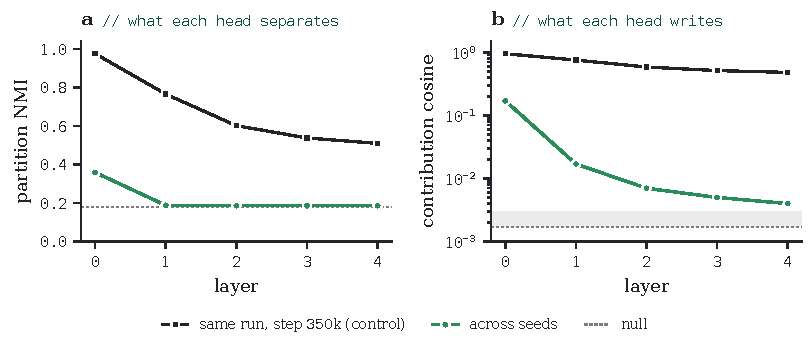
\includegraphics[width=\linewidth]{figures/fig-gpt2-seeds.pdf}
\caption[GPT-2 seed agreement by layer]{The GPT-2 concatenated-head seed
pair by layer: what each head separates (a, partition NMI on 32{,}768
rows) and what it writes (b, centered contribution cosine on 8{,}192
rows, log scale), across the two seeds and against the first run's own
checkpoint at step 350{,}000. Dotted lines are the nulls; the band in (b)
runs from the null's mean to its maximum. One seed pair.}
\label{fig:gpt2-seeds}
\end{figure}

Only layer 0 reproduces, at under a fifth of the control, and each of its
heads matches into the other seed's layer 0 on both measures. Layer 1
keeps its identity (19 and 20 of its 20 heads land in the other seed's
layer 1) while agreeing on almost nothing it separates or writes; layers
2--4 lose even that. The partition null is high, because plug-in NMI
between two 256-way partitions of 32{,}768 rows is dominated by bias, so
it cannot resolve the deep layers; against the tight contribution null
they sit two to four times above it, at about 1\% of the control, which is
real and negligible. The excess over the null is larger than on SONAR
($24\times$ against 5--11$\times$), almost all of it in layer 0, though
the GPT-2 arms also ran without the SONAR arm's calibration, and in this
pair the training noise, not the classifier, chose most layer-0
assignments throughout training (Table~\ref{tab:cfg-ste-gpt2};
Appendix~\ref{sec:calib}).

\subsubsection{What layer 0's lead is made of}

Three findings, detailed in Appendices~\ref{sec:l0size}
and~\ref{sec:entries}. Layer 0's larger contributions are all gain: it
receives the raw input, while its atoms are no larger than layer 1's
(Table~\ref{tab:gainatoms}), and at equal atom spread it still reproduces
$14\times$ better on GPT-2 and $23\times$ on SONAR. The stack costs
reproducibility at every layer: against flat-arm heads of the same size,
which see the same input with nothing downstream, the stack's layer 0
reproduces about $8\times$ worse and its deeper layers 19--49$\times$
worse, the reproducibility side of entanglement. Within layer 0 the atoms
decide: layer-0 entries are unequal by atom norm rather than usage
(Table~\ref{tab:entries}). On SONAR one head (54) holds 8 of the layer's
11 atoms above three times the median, reproduces at 0.844 against 0.249
for the next, and drives the within-layer correlation between agreement
and largest atom (Table~\ref{tab:bigatoms}); without it the layer-0 mean
falls only from 0.080 to 0.070. GPT-2's layer 0 has no such head: every
head carries a graded tail of large atoms, and agreement is narrowly
spread.

\subsection{Heads against a known factor: language, and what they encode instead}
\label{sec:lang}

Language is the corpus's one factor with free labels, which is why it is
measured, not because a head was expected to encode it: SONAR maps
translations to nearby points~\cite{sonar}, so language is a weak, residual factor of
the embedding. No head encodes it outright. The best reaches a partition
NMI of 0.18 against an attainable 0.875 (0.165 on the second seed), and no
head-health lever changes that (Table~\ref{tab:headlang}). Partitions do
carry the factor well above chance, and the hard code carries more of it:
3.5--3.9 times the softmax reference on null-corrected best-head NMI,
and 0.42 against 0.27 in a 32-head probe. Single cells and conjunctions of cells
detect language neighborhoods rather than identities (Finnish with
Estonian, Japanese with Korean), which matches an embedding in which
languages are weakly separated regions rather than directions
(Appendix~\ref{sec:langdetail}).

\paragraph{What the strongest head holds: topic and genre.} A semantic,
language-agnostic embedding should be organized by meaning, and its
strongest head is. Ranking layer-0 heads by $\eta^2$ and matching
partitions across runs (65{,}536 held-out rows):

\begin{center}\small\setlength{\tabcolsep}{4pt}
\begin{tabular}{@{}llrrl@{}}
\toprule
run & top head & $\eta^2$ & next head & match across runs \\
\midrule
\texttt{ste\_h76\_init01} (seed 42) & h54 & 0.117 & 0.062 & --- \\
\texttt{ste\_h76\_i01\_s43} (seed 43) & h14 & 0.122 & 0.068 & NMI 0.413 (others 0.010) \\
\texttt{ste\_h76} (unfixed init, seed 42) & h54 & 0.111 & 0.080 & NMI 0.355 (others 0.024) \\
\bottomrule
\end{tabular}
\end{center}

The topic head is the one head found in every run, the strongest
partition in each by nearly a factor of two. A different seed grows it at
a different index, and the same seed keeps its index across the
initialization fix. It is also the head that reproduces on contributions
(Appendix~\ref{sec:entries}), the exception to Section~\ref{sec:seeds}'s
finding that heads do not reproduce, though at NMI 0.41 against a 0.87
same-run control it is the same variable carved differently, not the same
partition. It also carries more language than almost any other head: in
seed 43 it is the most language-informative of all 380 heads (NMI 0.165,
Table~\ref{tab:headlang}) and in seed 42 the third (0.161), though
against an attainable 0.875 each of its entries still mixes many
languages. Decoded as deviations
from the head's mean atom, its entries read as topic and genre: crime
news, geopolitics and parliament, encyclopedic place description,
manufacturing, marketing, legislative text and entertainment. Contrastive
autointerp agrees, with every category of description above its
null (Appendix~\ref{sec:langdetail}). Testing whether heads are natural
variables therefore needs topic or genre labels, which this corpus does
not have.

\section{Hard codes on GPT-2 small: atoms in activation space}
\label{sec:gpt2hard}

A second line of straight-through runs, from the \texttt{headline}
branch, takes the hard code to GPT-2 small and adds what an embedding
substrate lacks: the fraction of GPT-2's loss recovered when the
reconstruction is spliced back into the model,
$(\mathrm{CE}_{\mathrm{ablate}} - \mathrm{CE}_{\mathrm{recon}})
/(\mathrm{CE}_{\mathrm{ablate}} - \mathrm{CE}_{\mathrm{clean}})$, with the
residual mean-ablated as the floor --- a lenient scale against an
ablation floor~\cite{gao2024}, so Table~\ref{tab:gpt2hard}'s caption also
gives the cross-entropies themselves. These runs model the residual stream
entering block 8, one block earlier than the GPT-2 runs of
Section~\ref{sec:seeds}, centered and scaled to unit mean square, on
FineWeb, and their $\fvu$ is unwhitened; they compare only with each other
and with SAEs trained on the same cache. Held-out evaluation uses
documents disjoint from training (520k tokens for the 40M-token runs, 65k
for one-epoch runs).

\paragraph{The design.} Relative to Section~\ref{sec:ste}, three things
change. Atoms are direct: signed vectors in activation space, with no
latent dictionary space and no decoder, so every atom is literally a
steering direction. Every layer, layer 0 included, classifies the unit
direction of what it corrects, and each layer's contribution is scaled by
the observed residual norm, clipped at $\lVert\mathbf{x}\rVert$, which
makes the model positively homogeneous ($f(\xi\mathbf{x}) = \xi
f(\mathbf{x})$ for $\xi > 0$). The straight-through temperature is
annealed early in training (Table~\ref{tab:cfg-gpt2-headline}). With
$5\times32$ heads of 32 entries the code is 800 bits per token, and its
only continuous numbers are the five layers' gains.

\begin{table}[htbp]\centering\small
\begin{tabular}{@{}>{\raggedright\arraybackslash}p{0.31\linewidth}%
>{\raggedright\arraybackslash}p{0.18\linewidth}%
>{\raggedright\arraybackslash}p{0.17\linewidth}rr@{}}
\toprule
model & atoms & code per token & $\fvu$ & \stackhead[r]{loss\\recovered} \\
\midrule
direct + gain + STE (10M tokens) & signed, in $\mathbb{R}^{768}$ & 800 bits + 5 gains & 0.217 & 97.0\% \\
\textbf{direct + gain + STE (40M tokens)} & signed, in $\mathbb{R}^{768}$ & 800 bits + 5 gains & 0.195 & \textbf{97.6\%} \\
concatenated heads + gain + STE & 48-dimensional blocks, shared decoder & 800 bits + 5 gains & 0.186 & 97.5\% \\
concatenated heads, $k{=}64$ & 48-dimensional blocks, shared decoder & 960 bits + 5 gains & \textbf{0.164} & \textbf{97.9\%} \\
\midrule
$\topk$ SAE, $k_{\mathrm{SAE}}{=}32$, $m{=}5120$ & --- & 32 coeffs + $\sim$276 bits & 0.189 & 96.2\% \\
$\topk$ SAE, $k_{\mathrm{SAE}}{=}128$, $m{=}5120$ & --- & 128 coeffs + $\sim$859 bits & 0.116 & 98.6\% \\
soft Ontologizer (1 epoch) & --- & 4960 mixture weights & 0.016 & 99.85\% \\
\bottomrule
\end{tabular}
\caption{GPT-2 small, residual entering block 8. Ontologizers: one pass
over 10M or 40M tokens, one seed (the 10M direct run's seed-43 replica
reaches $\fvu$ $0.219$ and $96.9\%$ recovered). SAEs: 10 epochs over the
10M-token cache with \texttt{sae.py}'s unwhitened objective; with
coefficients quantized to $\sim$5 bits each, the $k_{\mathrm{SAE}}{=}32$
SAE totals 556--588 bits at $\fvu$ $0.189$--$0.190$. Clean cross-entropy
3.806, mean-ablated 8.283; the 40M direct code reaches 3.914.}
\label{tab:gpt2hard}
\end{table}

A discrete 800-bit code recovers more of GPT-2's loss than a
$k_{\mathrm{SAE}}{=}32$ SAE both on the same 10M-token training cache
(97.0\% against 96.2\%, at $\fvu$ 0.217 against 0.189) and after one pass
over 40M tokens (97.6\% at 0.195), though with its 32 coefficients
quantized to $\sim$5 bits each (556--588 total bits against the
Ontologizer's $800 + {\sim}25$) the SAE leads on $\fvu$ per bit. Across
architectures, then, $\fvu$ does
not order downstream loss, while within the Ontologizer family on SONAR,
text fidelity was monotone in $\fvu$ (Appendix~\ref{sec:textfid}). Part
of such a gap can be mismatch rather than lost information: adapting the
downstream model to a frozen SAE closes 30--55\% of its cross-entropy
gap~\cite{chen2025lowrankadaptingmodelssparse}. With 64
entries per head (960 bits) the code passes the SAE on both measures.
Every layer contributes, entry usage stays near uniform, and the observed
gain is close to the best per-sample scale for each layer; one-epoch
ablations show that the gain-shape split and direct atoms each help,
direct atoms most, that annealing matters, and that giving the 40M
concatenated-head model per-layer decoders cuts $\fvu$ from $0.186$ to
$0.169$ ($97.3\% \to 97.7\%$ recovered) while dropping cross-layer
same-head coupling from $97\%$ to $6\%$
(Appendix~\ref{sec:gpt2ablation}).

\paragraph{Fibers.} A rank-$r$ local basis per entry, with coordinates read
linearly from the unit residual, turns the code into a discrete base point
plus $r$ numbers per head. ``Base only'' is the same model with the fibers
removed, which measures whether the discrete code still means what it
did:

\begin{center}\small
\begin{tabular}{@{}lrrr@{}}
\toprule
\stackhead{variant\\(1 epoch, direct + gain + STE)} & \stackhead[r]{extra\\numbers}
& \stackhead[r]{$\fvu$\\(base only)} & \stackhead[r]{loss\\recovered} \\
\midrule
base & 0 & 0.217 & 96.95\% \\
rank-4 fiber, fiber dropout 0.5 & 640 & 0.059 (0.274) & 99.4\% \\
rank-8 fiber, fiber dropout 0.5 & 1280 & 0.014 (0.304) & 99.9\% \\
rank-4 fiber, joint norm cap 0.2 & 640 & 0.180 (0.227) & 97.6\% \\
rank-1 radial fiber (gain per entry) & 160 & 0.148 (0.669) & 98.5\% \\
\textbf{frozen base, rank-4 fibers trained after} & 640 & \textbf{0.016 (0.215)} & 99.9\% \\
unconstrained fibers & --- & --- ($\sim$10) & --- \\
\bottomrule
\end{tabular}
\end{center}

Fibers recover far more than the SAE's advantage in $\fvu$, but they carry
hundreds of continuous numbers per token, more than the SAE's 32
coefficients, so this is not a matched-capacity comparison. The question
they raise is what keeps the discrete base honest. Unconstrained, the
fibers take over (base-only $\fvu$ about 10); fiber dropout holds the base
at 0.23--0.30 whatever the rank; and a joint norm cap guarantees it at the
cost of most of the fibers' value. Training the fibers after freezing the
base is best on both counts: the base is untouched by construction
(0.215), and the fibers reach the reconstruction of unconstrained joint
fibers. The mechanisms used in joint training suppress the fibers rather
than protect the base.

\paragraph{Describability cliff and lexical baseline.} Scoring entries by
how well an LLM judge, given a description written from activating contexts
in held-out documents, separates members from non-members (balanced
accuracy; chance $0.50$, document-split nulls $0.496$--$0.507$) reveals a
sharp drop with depth. On the 40M models, layer~0 averages $0.70$--$0.71$
across all entries ($0.91$ on an entry's top-scoring members, $0.65$ on
random members, and $0.55$ near the boundary), layer~1 falls to
$0.56$--$0.57$, and layers~2--4 sit at the $0.50$--$0.52$ null even with up
to 256 describing examples or 64-token contexts (set-level detection on
10-token bundles retains a small signal at layer~3, $0.556$ vs.\ a $0.505$
null). Even in layer~0, where 29--31 of the 32 heads track token identity
(alongside one position head at $1.3$--$1.8$ bits and two document heads),
a judge-free rule that sees only the current token's identity beats the LLM
judge on single cells ($0.75$ vs.\ $0.69$ on concatenated heads, $0.74$ vs.\
$0.71$ on direct atoms); intersecting two layer-0 heads raises balanced
accuracy against siblings by $+0.10$ on concatenated heads ($0.69 \to 0.78$,
mostly from lexical information) and by $+0.01$ on direct atoms ($0.71 \to
0.72$).

\paragraph{Steering, edit cost, and the random-projection null.} Single-head
edits on the 10M models are lightweight: setting one layer-0 head to its
mean entry everywhere costs $0.02$--$0.075$ nats of next-token KL (falling
from $0.063$ to $0.021$ on concatenated heads as head dropout rises from 0
to $0.5$), comparable to zeroing one active SAE latent ($0.055$ nats), and
swapping a single head from entry $j$ to $j'$ on the 40M models costs
$0.001$--$0.06$ nats at unit strength. Scored by how closely the steered
next-token distribution approaches entry $j'$'s empirical distribution
among the head's 31 alternatives (rank 0 best, $\sim$15 random; one head
each in layers 0, 2 and 4 over 128 windows), unit-strength swaps place
$j'$ at rank $3.5$--$6$, and $4\times$ swaps at rank $5$--$8$ against
$14$--$18$ for a norm-matched random direction. That specificity is not,
however, evidence that the learned entries carve meaningful variables: on
the 40M concatenated-head model (8 heads per layer, unit strength), steering
between the centroids of random-projection bins lands the target bin at
mean rank $0.21, 0.00, 0.44, 1.69, 1.27$ across layers 0--4, matching or
beating the learned cells' centroid steps ($0.56, 0.66, 0.75, 1.37, 1.28$)
and contrastive-entry steps ($0.71$--$1.94$; random directions
$14.2$--$16.9$). Because the downstream map from block~8 to the logits is
locally close to linear, any partition's cell-centroid differences steer
specifically toward that partition's cells.

\paragraph{Seed stability, replicated.} Matching heads across two seeds by
partition NMI, the partitions agree only in layer 0 (NMI 0.088 against
0.050 for unrelated heads within one run, and 0.002 under a row shuffle)
and not at all in layers 1--4 ($0.003$--$0.015$).
With direct signed atoms, the gain-shape split from layer 0, a different
site and a different objective, this repeats Section~\ref{sec:seeds}:
which entries share a head depends on the seed past the first layer.

\section{Dictionary geometry and the non-negativity constraint}
\label{sec:geom}

Two geometric facts frame this section (Appendix~\ref{app:geom}). Row
collinearity measured in the dictionary space is mostly gauge: 74--78\% of
each atom's energy lies in the decoder's null space, so dictionary
statistics should be computed after decoding (Appendix~\ref{sec:rowcos}).
And the selection rule shapes the dictionary less than training duration
does, while the last layer becomes inert once the error before it is
small (Appendix~\ref{sec:lastlayer}).

\subsection{The orthant forces a collinear dictionary}
\label{sec:gpt2}

Non-negativity binds through the Gram, not the null space. Two
non-negative vectors have a non-negative inner product exactly, so for
independent $\lvert\mathcal{N}(0,1)\rvert$ coordinates the chance pairwise
cosine is $2/\pi = 0.637$ (minimum $+0.58$ over 4000 draws), where signed
draws give 0.000. Dropping the absolute value (\texttt{--signed}) on GPT-2
layer 8, with the straight-through arm's shape, crossed with dictionary
width and trained to convergence (371{,}900 steps):

\begin{table}[htbp]\centering\small
\begin{tabular}{@{}lrrrr@{}}
\toprule
arm & $\bar\kappa$ (row cosine) & eff.\ rank & $\fvu$ & at step 90k \\
\midrule
signed, $e{=}1536$ & $+0.0009$ & 27.37 & \textbf{0.1540} & 0.2910 \\
signed, $e{=}768$  & $+0.0019$ & 26.95 & 0.1543 & 0.2942 \\
abs, $e{=}1536$    & $+0.3038$ &  9.15 & 0.1934 & 0.3962 \\
abs, $e{=}768$     & $+0.4543$ &  5.41 & 0.2927 & 0.4631 \\
concat, $d_{\mathrm{head}}{=}32$ & $+0.5353$ & 3.30 & 0.4155 & 0.8055 \\
\bottomrule
\end{tabular}
\caption{Non-negativity $\times$ width on GPT-2 layer-8 residuals,
held-out tail: geometry from the weights, $\fvu$ scored from each
checkpoint. No collinearity penalty is active in any arm.}
\label{tab:orthant}
\end{table}

Forced collinearity costs reconstruction. At $e{=}1536$ the non-negative
dictionary runs at a third of the signed effective rank and 26\% more
held-out error; at $e{=}768$, 90\% more. Across the five arms $\bar\kappa$
orders the error exactly at convergence (Spearman $+1.00$; $+0.90$ at
step 90k, where concat is the single inversion). The cost is an
interaction: narrowing $e$ costs 0.2\% with signed atoms and 51\% with
non-negative ones, so the wide dictionary buys room for the constraint
rather than capacity (Appendix~\ref{sec:rowcos}). That undercuts
Section~\ref{sec:disjoint}'s claim that head-disjointness is what $e > d$
buys, and no model attains head-disjointness in any case
(Appendix~\ref{sec:support}). The non-negative arm's gap at $e{=}1536$ grew
from 8\% at step 20k to 50\% at 200k and has since narrowed to 26\%
(Figure~\ref{fig:orthant-curves}), so it may be partly slower, but it has
not caught up by the end of a full run.

\begin{figure}[tp]\centering
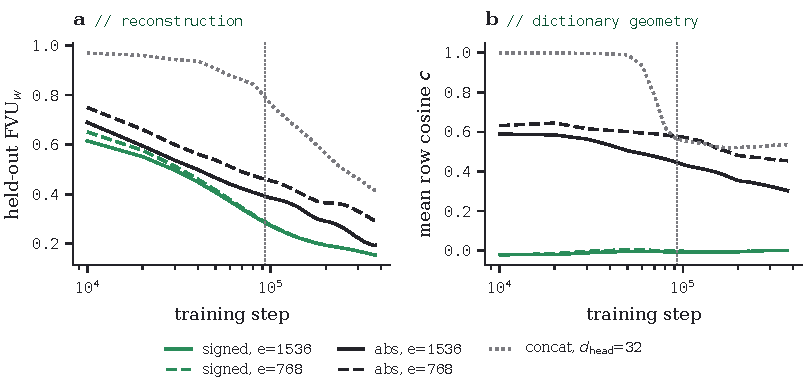
\includegraphics[width=\linewidth]{figures/fig-orthant-curves.pdf}
\caption{The orthant arms over training: held-out $\fvu$ scored from each
checkpoint (a) and mean within-head row cosine (b). The dotted line
marks step 90k. The signed arms coincide at both widths; \texttt{abs} is
behind at both, and further behind at the square decoder.}
\label{fig:orthant-curves}
\end{figure}

Removing the absolute value buys a decorrelated, near-full-rank
dictionary and lower error, roughly what the collinearity setpoint exists
to buy. Signed atoms give up two things: a subtractive feature is harder
to read as ``this concept is present'', and the $\lVert F\rVert_1 \geq h$
floor under \texttt{norm\_rows}, which rests on non-cancellation,
disappears. Concatenated heads at $d_{\mathrm{head}}{=}k{=}32$ under
non-negative atoms and constant temperature, which face a collapsed
tradeoff rather than a raised floor, are the worst arm here
(Appendix~\ref{sec:concatgeom}); giving each head's block headroom
($d_{\mathrm{head}}{=}48 > k{=}32$) and annealing the temperature reverses
that ranking in Section~\ref{sec:gpt2hard}.


\section{Formal reading: heads as causal variables}
\label{sec:formal}

The steering frame has a natural formalization in the causal-abstraction
vocabulary~\cite{rubenstein2017,beckers2019,geiger2021,geiger2025}. An
abstraction relates two causal models through a map between their states
and a map between their interventions, so stating the frame means naming
both models, and it shows what each instrument in the battery does and
does not estimate.

\paragraph{Definitions.}
The high-level model is the Ontologizer's forward pass, read as a causal
model over the input and the heads: each head $(\ell,i)$ is a candidate
\emph{variable} with value space $\{1,\dots,k\}$, $\mathbf{x}$ is a
parent of every head, and with residual forwarding every earlier head is
a parent of every later one, since layer $\ell{+}1$'s classifier reads the
residual written by layers $\le \ell$. These edges belong to the code:
unlike those of transcoder circuits~\cite{dunefsky2024}, which pass
through a model's own sublayers, they describe how the code refines one
representation, not how the encoder computes it. \texttt{withArgs}
set-interventions are this model's hard interventions:
$\mathrm{do}[(\ell,i){=}j']$ forces the head's assignment while leaving all
non-descendants untouched by construction, and marginalizing the
continuous intermediates out of the forward pass is an exact
transformation by construction~\cite[Thm.~10]{rubenstein2017}. A soft
head's state is a point of its simplex, so reading it as one of $k$ values
is a lossy value merge~\cite{geiger2025}, and a set on a soft head is a
steering intervention rather than an interchange. The low-level model is
the encoder whose embeddings the code reads, and the map between their
states is $\mathrm{assign}$, which sends an embedding $\mathbf{x}$ to its
per-head assignments. Whether the head model abstracts the encoder under
$\mathrm{assign}$ is an approximate-abstraction
question~\cite[Def.~41]{geiger2025}, and the abstraction cannot be a
constructive one~\cite{beckers2019}, since every head reads the same
embedding.

\paragraph{What the instruments estimate.}
Input-space steps are not interventions such an abstraction maps; they
score control of the head model, not whether the encoder computes with
the heads~\cite[Sec.~3.7]{geiger2025}. \texttt{steerembed.py}'s
realization rate checks one coordinate of the condition that a stepped
input's code equal the code under $\mathrm{do}[(\ell,i){=}j']$, so a rate
below 1 already rules out an exact transformation that maps the step to
that do. Its collateral counts the other heads that change against the
\emph{unsteered} code, which in a stack includes the downstream
reclassification the do itself would cause. \texttt{steerfid.py}'s
cycle-consistency gain asks the same of a text-level implementation,
through the closed loop $\mathrm{assign} \circ \mathrm{encode} \circ
\mathrm{decode}$: it is a normalized activation gain net of a random
control, not an interchange-intervention accuracy~\cite{geiger2022},
since it patches nothing in from a source input, and the loop's
$\sim$13\% unsteered round-trip survival (Section~\ref{sec:steer}) limits
how often an exact intervention could be observed through it.
Seed-to-seed matching asks whether two runs' $\mathrm{assign}$ maps agree
up to relabeling. What the softmax leaves unidentified in principle is the
per-head entry order (permutation) and any logit gauge the temperature
absorbs; what must be reproducible for the heads to be properties of the
data rather than of one run is therefore the partition itself and the
decode directions up to relabeling. Section~\ref{sec:seeds} measured
exactly that on the hard code, on SONAR and GPT-2. Past layer 0 no head
reproduces, and nothing measured there shows that the layer does either:
per-layer subspaces agree only as much as each model agrees with the
data's principal directions. Whether a layer reproduces as a variable
merge of its heads~\cite[Def.~37]{geiger2025}, of which the per-head
variables are a seed-dependent factorization, needs a whole-layer
comparison that translates one seed's layer code into the other's. Layer
0 partly reproduces, on SONAR almost entirely through a single large-atom
head.

\paragraph{Why the cascade costs reproducibility.} The stack's
reproducibility deficit at matched head size
(Section~\ref{sec:l0size}) and its intervention collateral
(Section~\ref{sec:entangle}) are one fact under this reading. A head's
value is a function of its own input, and every head past layer 0 takes
as input the residual that upstream heads leave; a different upstream
solution changes what any downstream variable is \emph{about}. Even layer
0, whose input is the data, is pinned only partly: its heads are trained
jointly with everything downstream of them, so which partition of the raw
input is best depends on what the later layers will do with the error.
A flat layer has neither dependency: its heads are more reproducible at
equal size and realize interventions far more reliably, with half the
collateral. They are still not independently addressable --- the hard
code's heads sit almost on their decision boundaries in either shape ---
so the cascade compounds an entanglement that the code already has.

\paragraph{Metric hygiene.}
Claims about decode-direction geometry should not depend on an arbitrary
choice of inner product, a point Park et al.\ make for language-model
representations, which they read under an estimated causal inner
product~\cite{park2025}. The contrast-set result does not depend on it:
under the
training objective's inverse-variance metric (a whitening of the data,
not their causal inner product) the Ontologizer's
within-head repulsion strengthens ($-24.4$ vs.\ $-17.6$ raw) and both
rivals' signatures are unchanged. Two further rules emerged. Measure in
output space, not in the dictionary space, whose null-space component is
unconstrained (Section~\ref{sec:rowcos}) and is exactly the kind of
causally disconnected direction that makes subspace patching
misleading~\cite{makelov2023}. And separate a layer's gain
from a head's atoms before attributing anything to head size: across
layers, size is the gain, and the gain is the layer
(Section~\ref{sec:l0size}).

\paragraph{Composition.}
A variable reading earns little if interventions on two heads interact
uncontrollably. Measured additivity of decode deltas on
\texttt{resid\_nc} (\texttt{compose.py}, whitened metric, medians over
pairs):

\begin{center}
\begin{tabular}{@{}lrrrr@{}}
\toprule
stratum & pairs & cos & rel.\ err & later layers \\
\midrule
same-layer L0 & 28 & 0.959 & 0.350 & 4 \\
same-layer L1 & 28 & 0.947 & 0.354 & 3 \\
same-layer L2 & 28 & 0.967 & 0.259 & 2 \\
same-layer L3 & 28 & 0.996 & 0.092 & 1 \\
same-layer L4 & 28 & 1.000 & 0.019 & 0 (numerical floor) \\
cross-layer (earlier $=$ L0/L1) & 42 & 0.97--0.98 & 0.20--0.23 & \\
cross-layer (earlier $=$ L2/L3) & 18 & 1.00 & 0.02--0.04 & \\
\bottomrule
\end{tabular}
\end{center}

Three observations. (i) Joint interventions point where the summed
singles point everywhere (median cosine $\ge 0.95$ in every stratum):
\texttt{withArgs} interventions compose approximately additively. (ii) The
non-additive component is entirely attributable to downstream
reclassification: it decays monotonically with the number of layers below
the intervention and hits the numerical floor when there are none (the
measured $0.019$ is float32 rounding amplified by the decoder
cancellation, ${\sim}3{\times}10^{-6}$ in float64). (iii) Cross-layer
pairs compose \emph{better} than same-layer pairs at matched depth: a
set-intervention is immune to upstream perturbation, so cross-layer
interaction is one-way. Note the contrast with
Section~\ref{sec:entangle}: \texttt{withArgs} sets a head directly and
composes well, while an \emph{input-space} push reaches every head and
disturbs most of them. The downstream reclassification that is a 5--35\%
correction to a set-intervention is the dominant effect of an input-space
one.

\section{Preliminary conclusions}

\begin{enumerate}
\item \textbf{Contrast-set structure is real, and it is what the
architecture buys.} Trained softmax heads' decode directions repel (96\%
of heads below null), and hard-code heads' decoded atoms are orthogonal
to slightly repelling: each head holds well-separated alternatives. This
is invisible to reconstruction metrics and to per-latent probes.
\item \textbf{The other designed orthogonality did not emerge: heads share
their coordinates.} No trained model partitions its dictionary space
between heads; the support overlap sits at or above a coordinate-shuffle
null in every model, each head's usage covers 52--98\% of the coordinates,
and this holds for the part of each atom the decoder sees as well as for
its null-space part. Only very long training (8.27M steps) moved it, by
sparsifying each head's profile rather than separating heads. A static
reading of the dictionary cannot assume disjoint heads; concatenated heads
are the only route to them, by construction.
\item \textbf{A discrete ontology is possible, but not with the softmax
architecture's readout.} The softmax model's argmax is not its code (at
least 77$\times$ from the best 800-bit code for \texttt{resid\_nc}, nine
orders of magnitude on \texttt{softmax\_shm}). A straight-through arm
with $2.4\times$ the heads makes the discrete code the model: with its
four per-layer gains pinned it is a pure 1900-bit code at $0.158$. At the
same total rate the converged $\topk$ SAE and the single-layer hard
variant cannot get below $0.236$--$0.273$ however their coefficients are
coded, but a coarsely quantized L1 SAE, entropy-coded, reaches $0.129$
averaged over rows and $0.152$, level with the hard code, held to 1900
bits on every row; averaged over rows the hard code leads every SAE only
when each support is charged its fixed-length cost (0.158 against 0.180),
because its own entries are used almost uniformly and an L1 SAE's latents
are not.
It sits $3.1\times$ above the Gaussian reference for its rate, so at least
that far from the data's distortion--rate function, a limit over long
blocks of samples that a code describing each sample alone need not be
able to reach~\cite{cover2006}. It needed a
temperature matched to the logit scale, relative logit noise, a rescaled
entropy bonus, and an initialization fix worth a third of its error.
\item \textbf{The discrete code holds up downstream.} On GPT-2 small, an
800-bit hard code with signed atoms in activation space and gain-shape
on every layer recovers 97.6\% of GPT-2's loss, more than a $k_{\mathrm{SAE}}{=}32$ SAE
at nearly the same $\fvu$ (96.2\%), and 64 entries per head pass it on
both measures. Across architectures $\fvu$ does not order downstream
loss. Fibers on top of a frozen discrete base recover almost all the rest
(99.9\%) while leaving the base exactly as it was, so a discrete ontology
and a near-lossless reconstruction need not trade against each other ---
at the price of hundreds of continuous numbers per token.
\item \textbf{Reconstruction is the price sheet, not the verdict, for
soft codes.} Unstructured codes reconstruct $\sim$50$\times$ better at
matched coefficient budgets, and the per-head simplex constraint alone
costs $\sim$30$\times$; text fidelity is a monotone function of $\fvu$
and adds no independent axis.
\item \textbf{The residual cascade is measured on both sides of the
ledger.} For: $1.79\times$ lower error than a flat layer at equal bits,
parameters and near-uniform head usage on both sides, sourced in the pairing of each stage's
input with the sample's own error (not utilization, conditioning, or the
gain side-channel; deep supervision, which only the stack has, is not yet
ruled out). Against: an input-space intervention disturbs 66\%
of the stack's other heads against 33\% of a flat layer's, and realizes
its target on 37\% of rows against 99.6\% --- in both, collateral equals
a random step's, because the hard code's heads sit almost on their
decision boundaries; and
at equal head size the stack's heads reproduce across seeds several
times worse than flat heads at every layer, layer 0 included. The
single-layer softmax variant \texttt{g160softmax} matches \texttt{resid\_nc} on
reconstruction, but a config-matched softmax Ontologizer reaches
$6\times$ lower error, on rows no model trained on as on the tail, so the
reconstruction verdict against the stack was checkpoint-specific.
\item \textbf{Steering works in embedding space and the text cycle hides
it.} The decode direction realizes a target entry on 82\% of rows for the
softmax model at strength 0.25, against a 3\% chance rate, while the
text round trip can observe at most $\sim$13\% of perfect interventions.
The soft code is the more steerable at low collateral; steerability does
not track reconstruction, and the classifier's own gradient is the right
direction only where the input reaches the classifier directly.
\item \textbf{Individual heads past layer 0 are not reproducible, and
layer 0 only partly.} Seeds agree on the error to four digits but not
on the reconstruction: their residuals correlate at 0.30, where an SAE's
seeds reach 0.83. Past layer 0 they agree on nothing that identifies a
head --- partitions, contributions, subspaces beyond the data's, or
Grams --- each tested against a same-shape null, on SONAR and on GPT-2,
and again under the direct-atom design of Section~\ref{sec:gpt2hard},
though within one run every head persists. Layer 0 reproduces at
under a fifth of a same-run control. Its lead over the deeper layers is
not atom magnitude: its atoms are no larger, and its larger contributions
are its gain, which is a property of the layer. Within layer 0, heads
with outsized atoms are the reproducible ones --- on SONAR almost
entirely one head. This remains the most consequential result for the
steering frame: a head that is not the same head on the next run cannot
be named, and every per-head claim here inherits that.
\item \textbf{Entries contribute near-equally except where the input is
raw.} In layers 1--3 every entry carries close to its share (Gini
0.06--0.15, no dead entries); layer 0's entries are unequal (Gini
0.33--0.59) because its atom norms vary widely inside heads, while
usage stays near-uniform. The flat arm shows the same pattern, so it
belongs to classifying the raw input.
\item \textbf{Heads follow what the embedding encodes: meaning before
language.} The strongest head encodes topic and genre, as a
language-agnostic semantic embedding should be organized, and it is the
one head that recurs across seeds. Language, the
one factor with free labels, was a probe rather than an expected
variable: it is carried as neighborhoods across heads, never by one
head, consistent with languages being weakly separated regions of SONAR
space. On that probe the hard code carries 3.5--3.9 times what the softmax
reference does, so partitions do align with known factors; a test of
whether heads are natural variables needs topic or genre labels.
\item \textbf{Per-latent lenses mis-measure classifier codes.} Sparse
probing ranks the Ontologizer worst while partition-level analysis finds
verified causal language heads; detection F1 is $\sim$80\% explained by
code density and more by how many languages a latent's top rows span,
which moves with it, and on features spanning as many languages as
random rows do, the sparse codes' lead over the Ontologizer falls to 0.10
or less.
Parameter-space decodes are instances, not descriptions, and must be
taken as deviations from the head mean to be legible at all, as the
geometry of categorical concepts predicts: a category's value vectors
share their parent's component and separate only as differences from
it~\cite{park2025}.
\item \textbf{Non-negativity is expensive in geometry and in error.} It
forces a collinear, low-effective-rank dictionary (a third of the signed
rank) and costs 26\% of held-out $\fvu$ at the wide dictionary, 90\% at a
square decoder; row collinearity orders all five GPT-2 arms by error at
convergence. Signed atoms decorrelate the dictionary and reconstruct
better at either width. Dictionary statistics computed in the dictionary
space rather than after decoding are mostly gauge.
\item \textbf{Every measure in this architecture needs a null of the same
shape.} Non-negativity and the layer-dependent gain put structure into
every floor. Three of four seed-reproducibility measures, the HSIC head
dependence, the null-space readings, and the apparent size effect on
reproducibility each reversed or dissolved under the right control.
\end{enumerate}

\section{Follow-up investigations}
\label{sec:followup}

Ordered by relevance to the steering goal.

\begin{itemize}
\item \textbf{Head identifiability first.} Before naming heads, make them
reproducible or establish which are. The softmax Ontologizer's
partitions are now compared across seeds too, and at 370k steps match
essentially nothing (Appendix~\ref{sec:softseed}). A $k{=}128$ pair
sharpens the problem. Two architectures trained from the same seed, one
decoding its atoms and one with direct atoms, share their partitions
head for head (matched NMI 0.18, every head matched to the head at its
own index), while each architecture across seeds reaches 0.064 against
a 0.059 null. Seed replicas see the same data in the same order, so the
seed acts only through the initialization and the training noise; it,
rather than the data or anything after the classifier, largely fixes
what a head carves, as in toy networks, where seeds trained on identical
data implement one algorithm through different
features~\cite{chughtai2023}. Classical identifiability results point to
two routes out: selecting among trained seeds by pairwise cross-seed
agreement without labels, as Unsupervised Disentanglement Ranking scores
models by their median alignment across seeds~\cite{udr2020} (where
three or more conditionally independent views of a discrete variable
identify its distribution up to label permutation~\cite{allman2009},
though here the heads are the candidate views rather than fixed ones, and
even sparse binary codes need nonlinear dynamics and radial richness
when learned from static marginals~\cite{hillar2015}); and breaking the
static marginal symmetry with paired observations, where temporal
contrast~\cite{pcl2017}, sparse transition priors~\cite{slowvae2021},
shared factors across corruptions~\cite{locatello2020}, auxiliary
conditioning~\cite{ivae2020}, or contrastive alignment of conditional
balls~\cite{zimmermann2021} give identifiability up to permutation.
Initial probes on the sentence-split cache \texttt{mc4\_sent16}
(Appendix~\ref{sec:seedsdetail}) bound and test the second route: linear
ridge regression of $\mathbf{x}_{t+1}$ on $\mathbf{x}_t$ reaches
$\mathrm{FVU}_{\mathrm{next}}{=}0.896$ (about 10\% of next-sentence
variance explained, the ceiling for any function of $\mathbf{x}_t$
alone); adjacent sentences concentrate strongly in direction (raw cosine
AUC 0.923 vs.\ 0.685 in whitened distance, which norm variance
dominates), yet existing heads switch entries on 92.2--98.1\% of adjacent
pairs with off-diagonal transition concentration $\kappa \le 0.081$; and
penalizing cross-sentence assignment disagreement on 38 slow heads
collapses them to 0.04--0.09 bits for $s_{\mathrm{pair}} \ge 10^{-4}$ even
under $\mathrm{KL}_m{=}5\times10^{-4}$, motivating a hinged Fano
conditional-entropy lower bound $[H(P_b \mid P_a) - H_{\mathrm{floor}}]_+$
that turns off once the transition table is sparse. Other candidates:
replicas of \texttt{resid\_nc\_hm} to its full 4.4M steps and of
\texttt{g160softmax}; whether large-atom heads' reproducibility can be
extended by training pressure; whether the $k{=}2$ arm's one-bit heads
reproduce better than 32-way ones; what lets the topic head recur when no
other head does (at $k{=}128$ a dominant layer-0 head recurs with a third
to a half of its agreement); whether a per-head router's gain is what
reproduces, since on GPT-2 the router doubles contribution agreement
while switching off the last two layers; and a GPT-2 flat arm, so the
matched-size comparison of Section~\ref{sec:l0size} has a second dataset.
\item \textbf{Bring the rest of the GPT-2 hard code onto this branch.}
Direct atoms are ported (Appendix~\ref{sec:gpt2ablation}), but
\texttt{resid\_first} and \texttt{gain\_clip} are not, so
Section~\ref{sec:gpt2hard}'s runs still reproduce only on the
\texttt{headline} branch. On SONAR, $5\times54$ heads at $k{=}128$
(1{,}890 bits, matching the $k{=}32$ stack's 1{,}900) converge to twice
its error ($\fvu$ 0.31--0.32 against 0.1535, two seeds each), with direct
atoms 0.009 ahead of decoded ones. Both codes are full, so the gap is not
utilization; but the temperature, learning rate and mean-entropy weight
were tuned at $k{=}32$ and carried over, and need retuning before the gap
reads as a property of $k$. Direct atoms also make steering literal, a
set-intervention adding $g_\ell(\mathbf{a}_{ij'} - \mathbf{a}_{ij})$ at
one layer, and that has not been measured.
\item \textbf{Per-layer decoders vs.\ width-matched shared decoders.}
Early direct-atom pilots on GPT-2 showed $<0.007$ $\fvu$ gain from
per-layer decoders, which had placed them under closed items. On the
40M-token concatenated-head run (Appendix~\ref{sec:gpt2ablation}), giving
each layer its own decoder instead cuts held-out $\fvu$ from $0.186$ to
$0.169$ ($97.3\% \to 97.7\%$ loss recovered) and drops cross-layer
same-head coupling from $97\%$ to $6\%$, near the $3\%$ chance floor,
showing that the coupling was an artifact of head $i$'s slice being read
through one shared decoder block across all five layers. Because five
decoders multiply decoder parameters by $l{=}5$, a shared decoder matched
in total width ($d_{\mathrm{head}}{=}240$) is the control still owed.
\item \textbf{Fibers on a frozen base.} The two-stage recipe kept the base
exact and matched unconstrained fibers' reconstruction on GPT-2. Fibers
are ported, but no SONAR run has used them; the recipe should be the
default there, scored at matched continuous capacity against SAEs
(rank-1 radial fibers already sit at 160 numbers per token).
\item \textbf{Remeasure on the fixed initialization.} Entanglement and
the gain and blend ablations ran on the shipped initialization, which
was $1.84\times10^8$ off at step 0 and left 10\% of the code unused.
\item \textbf{The steering overlay at scale.} Supervised vectors are now
scored on the model's own categories (Section~\ref{sec:steer}) and, for
\texttt{resid\_nc\_hm}, on an external concept, language
(Appendix~\ref{sec:steeroverlay}). Still open: the language overlay on
the hard code and the flat arm; bilinear eigenfeatures; per-entry effect
consistency across contexts, which for SAE features is partly predictable
before intervening~\cite{duan2026}; and the flat arm's near-perfect
realization, halved collateral and better reproducibility weighed
against its $1.79\times$ reconstruction cost. Collateral needs a lever
more than a better direction. It is direction-blind even with the
cascade excluded: every Ontologizer's decode direction, linearized
within its own layer, flips other heads at a random step's rate. In
decoded text too, removing what a head wrote costs no more than a random
step of the same length. The hard code's heads sit close to their
decision boundaries: linearized within its layer, a random step of
$0.25\lVert\mathbf{x}\rVert$ flips 30\% of the other heads in that
layer, and distance from the boundary looks like the lever.
\texttt{ste\_k2\_h380}, five layers of 380 binary heads, is the hardest
Ontologizer to disturb. The same step flips 13\% of its other heads to
first order, and measured through the stack it moves 17--19\% of them in
every direction, random included, against 66\% for the 32-way stack. Its
logit margins are 34 times the 32-way stack's, but that ratio is not the
evidence: they doubled between steps 370k and 739k while the first-order
share held, so the logits' scale grew with them. The step count explains
neither gap: at step 370k, the 32-way stack's whole run, the first-order
share and the measured collateral were both the same. Nor does the
mean-entropy weight, which matches the 32-way stack's per head ($\mathrm{KL}_m$ averages over
heads, and $5\times10^{-4}$ over 380 heads is $10^{-4}$ over 76). But the
arm trained on one seed and at half the batch size, so on a noisier
gradient at every step, and the comparison does not isolate the number
of entries.
\item \textbf{Task reconstruction.} Recover what each head classifies.
Head-level autointerp, which describes a head from its entries' texts
side by side and scores blinded assignment against sibling entries,
finds no above-chance signal at 20 heads per condition, on heads not
screened for identifiability (Appendix~\ref{sec:headautointerp}). Scored
by modularity on a nearest-neighbor graph of the residual each layer
classifies, the softmax Ontologizer's layers 1--4 are two to three times
as modular as size-matched regroupings of their entries; neither the
discovered groups nor the trained heads of a Matryoshka
SAE~\cite{bussmann2025} are, on matched
prefix-residual graphs (one checkpoint each;
Appendix~\ref{sec:modularity}). Still open:
partition-vs-label-library MI, led by topic and genre (from a labeled
corpus or unsupervised topic clusters) since those are what the
embedding is organized by, with length, formatting/noise and script as
secondary factors; head-level autointerp on heads that pass the
identifiability bar, at a sample large enough to separate from its
null; and FLORES parallel-text invariance to split content heads from
form heads. Run each identically on Ontologizer heads and
\texttt{g160softmax}'s heads.
\item \textbf{Hierarchy as MoE routing.} Conditional MI between
successive layers' partitions tests whether depth builds compositional
tasks; \texttt{forward="labels"} at the fixed initialization tests the
pairing account from the other side. Pairwise effective
information~\cite{hoel2013} bounds the edges of
Section~\ref{sec:formal}'s causal graph: on the hard code, forcing a
head to one of its live entries moves any single downstream head's
choice by about 0.01 of a possible 5 bits, at every depth, though 11--16
times more than the pair co-varies naturally. Whether that influence is
spread thinly or joint across sources, which pairwise measures cannot
see, is open.
\item \textbf{The collinearity setpoint's mechanism.} The one lever that
buys steerability acts on a statistic that is mostly gauge; repeat it on
the decoded statistic, and on signed dictionaries.
\item \textbf{Penalize head overlap where a decoder cannot absorb it.}
Trained as a loss term, $\omega$ reaches its target in the dictionary
space and nowhere else: the partition moves into the decoder's null
space, or a near-null one when the decoder is square
(Appendix~\ref{sec:support}). The penalty has to act on decoded atoms, or
on direct atoms, which have no decoder. The $k{=}128$ direct runs trained
only at $s_\omega{=}10^{-6}$, too weak to move $\omega$, where on GPT-2 it
takes hold from $10^{-5}$. Output coordinates are not privileged axes (a
product quantizer does better on a learned rotation of a space's
coordinates than on the raw ones~\cite{ge2014}), so a disjoint-coordinate
partition there is a strong and somewhat arbitrary constraint, but it
cannot be faked. Concatenated heads remain the only
route to disjoint support.
\item \textbf{Logit-scale control for straight-through training.}
Without per-head logit normalization (\texttt{logit\_norm}), classifier
logits adapt their scale to cancel a temperature anneal after the early
transient (Appendix~\ref{sec:gpt2ablation}). Normalize logits per head, or
control $t$ against a spread$/t$ setpoint, in place of the hand-matched
temperature, or add a term that pushes the logits to commit, the
counterpart of the commitment loss by which VQ-VAE ties an encoder's
scale to its code~\cite{vandenoord2017}.
\item \textbf{Codes trained for their rate.} The operational rates price
codes that were never trained for a codec: the hard code's entries are
used almost uniformly, the most expensive usage to entropy-code, and no
SAE was trained with quantized coefficients. Training each against its
entropy-coded rate --- an entropy penalty on the hard code's usage,
quantization-aware SAEs swept through the 1{,}900-bit region --- would
compare the architectures rather than these models.
\item \textbf{Winner dropout for the one-layer variants.} \texttt{g160top1}'s
29\% dead latents are within-head winner-take-all starvation. They
survived Gao et al.'s auxiliary loss on dead latents~\cite{gao2024}
(\texttt{aux\_k} 512, on throughout training), which gives a dead latent
gradient without making it win its head. Two older remedies are the
alternatives to test beside winner dropout: k-sparse autoencoders starve
the same way at low $k_{\mathrm{SAE}}$ and avoid it with a budget that
falls from 100 to its target over the first half of
training~\cite{makhzani2014}, here a top-$k_{\mathrm{sel}}$ per head
annealed to top-1; and neural codecs re-seed a codeword whose running
usage falls too low at an input from the current batch~\cite{zeghidour2021},
as \texttt{sae.py}'s neuron resampling already can.
\item \textbf{Trained truncatability.} A deviation-sparsity penalty at
training time would show whether the soft Pareto curve can shift left,
as training against several sparsities at once makes a $\topk$ SAE's
code progressive~\cite{gao2024}.
\item \textbf{Rung composition and frontier fill.} \texttt{groups+prefixes}
(2a+3) is now trained, as \texttt{m5120\_g160top1\_p5} ($\fvu$ 0.294), for
the modularity control above, but is not yet on the ladder. Still to run:
the one-layer variants at $m{=}11264$, the mid-range $\topk$ sweep
($k_{\mathrm{SAE}} \in \{512, 2048\}$), and random-support and
nonnegative-LS refit controls, the second being the positivity-constrained
refit of Gao et al.~\cite{gao2024}.
\item \textbf{Closed.} HSIC head independence (heads are already
independent), the HSIC penalty's freeze (real, and the biased
estimator's: only a frozen head escapes its floor;
Appendix~\ref{sec:freeze}), decoder sparsification and bias (no
structure; $<1\%$),
code-forwarding alongside the residual, input whitening (subsumed by
initialization), and entropy-pressure rescaling across shapes
(likewise). The \texttt{resid\_nc} layer-4 freeze is
explained by saturation, and the probe correction leaves it unchanged;
the two anomalously coherent heads (L2h25, L3h28) remain to inspect.
\end{itemize}


\section*{Reproducibility}

% sloppypar: the paragraph is mostly unbreakable script names, so its lines
% are set loose (five underfull warnings) rather than into the margin
\begin{sloppypar}
All code is available at \texttt{https://github.com/WakaruLabs/ontologize}.
The evaluation protocols are root-level scripts
(\texttt{sae.py}, \texttt{pareto.py}, \texttt{headstruct.py},
\texttt{headcoh.py}, \texttt{splitting.py}, \texttt{textfid.py},
\texttt{langprobe.py}, \texttt{refit.py}, \texttt{steerfid.py},
\texttt{compose.py}, \texttt{autointerp.py}), driven by the
\texttt{sae\_ladder.sh}, \texttt{sae\_evals.sh}, and
\texttt{autointerp\_run.sh} runners (idempotent, crash-resumable systemd
user units; judge calls rate-metered). The straight-through arm and its
diagnostics live in \texttt{experiments/ste-arm/}
(\texttt{train\_ste.py}, \texttt{steerembed.py}, \texttt{blendablate.py},
\texttt{gainablate.py}, \texttt{inputgeom.py}, \texttt{dictgeom.py},
\texttt{lastlayer.py}, \texttt{partition.py}, \texttt{headcontrib.py},
\texttt{entryshare.py}, \texttt{bigatoms.py}, \texttt{headlang.py},
\texttt{headscript.py}, \texttt{headeta.py}, \texttt{embedgeom.py},
\texttt{decodehead.py}, \texttt{coordfvu.py}, \texttt{make\_zca.py}); its
notebook \texttt{experiments/ste-arm/notes.md} records every run's command
and the superseded readings. The sentence-split cache and next-sentence
transition probes live in \texttt{experiments/sentence-split/} and
\texttt{experiments/next-sentence/} (\texttt{eval\_next.py},
\texttt{transitions.py}, \texttt{train\_pair.py}). The GPT-2 hard-code runs of
Section~\ref{sec:gpt2hard} live in \texttt{experiments/gpt2/}
(\texttt{train\_onto.py}, \texttt{diagnose.py}, \texttt{seedstab.py}; notes
in \texttt{DIRECT\_GAIN\_STE.md} and \texttt{results/README.md}, with the two
headline runs' configs, diagnostics and loss curves) and need the
\texttt{headline} branch's code. The curated test suite pins each protocol's
statistics against planted-structure synthetics. Artifacts live under
\texttt{data/out/sonar/} and \texttt{data/out/gpt2\_l8/}. At most three
straight-through runs fit concurrently on one 24\,GB device.
\end{sloppypar}

\section*{Acknowledgements}
Design, typesetting, and editorial production of this preprint are by
The Flock Capital Research Department, whose error-diffusion pipeline
also printed the plates.

\printbibliography

\vspace{20pt}
\noindent\plate{
\includegraphics[width=\dimexpr\textwidth-0.8pt\relax]{figures/end-ridge.png}}\\[3pt]
\mutedlabel{ridge \textperiodcentered{} seed 32 \textperiodcentered{} the same pipeline, closing the file}

\appendix

\section{Notation}
\label{app:notation}

This appendix collects the symbols used throughout, with where each is
defined.

\paragraph{Conventions.}
Lowercase italic letters are scalars ($t$, $g_\ell$), bold lowercase
letters vectors ($\mathbf{x}$, $\mathbf{a}_{ij}$), uppercase italic
letters matrices ($W_{\mathrm{dec}}$, $D_i$), and sans-serif letters
tensors of rank three or more ($\mathsf{D}$, $\mathsf{P}$). A subscripted
object takes the font of what it is: $p_{nij}$ is an entry of
$\mathsf{P}$, $\mathbf{p}_{ni}$ a vector slice of it, and
$D_i := \mathsf{D}_{i\cdot\cdot}$ a matrix slice; where a lowercase entry
would read as a count, it is bracketed, as in $[\mathsf{K}]_{nij}$.
Batching adds a rank: one sample's assignments are
$P \in \mathbb{R}^{h\times k}$, a batch's
$\mathsf{P} \in \mathbb{R}^{b\times h\times k}$. Vectors are columns, so a
matrix acts on the left ($W_{\mathrm{dec}}\mathbf{r}_\ell$, with
$W_{\mathrm{dec}} \in \mathbb{R}^{d\times e}$ mapping $\mathbb{R}^e$ to
$\mathbb{R}^d$); a batch stacks its samples as rows
($X \in \mathbb{R}^{b\times d}$), so a batched product carries a
transpose, $\hat{X} = R\,W_{\mathrm{dec}}^\top$, or is written as function
application, $\mathrm{dec}(R)$. Sets are calligraphic
($\mathcal{S}_n$, $\mathcal{G}$). Named statistics, losses and operators
are roman ($\fvu$, $\mathrm{MSE}$, $\mathrm{KL}_m$, $\mathrm{dec}$,
$\mathrm{sg}$), as are $H$, entropy, and $L$, the loss; the paragraph
around Eq.~\eqref{eq:realized} follows information theory in writing
random variables in uppercase. A hat marks a reconstruction
($\hat{\mathbf{x}}_\ell$), a tilde a noised quantity
($\tilde{\mathsf{F}}$, $\tilde{\mathbf{f}}_i$), a bar a mean
($\bar{\mathbf{p}}_i$, $\bar\kappa$), and a prime on an index a second
index of the same kind ($i'$, $j'$). $\odot$ is the elementwise product
and $\oplus$ concatenation. The cosine similarity of two vectors is the
cosine of the angle between them,
$\cos\angle(\mathbf{a}, \mathbf{b}) :=
\langle\mathbf{a},\mathbf{b}\rangle / (\lVert\mathbf{a}\rVert\lVert\mathbf{b}\rVert)$,
so that $\cos$ keeps one argument; $\lvert\cos\angle\rvert$ alone is its
absolute value for the pair in context. $\mathbb{E}$ is an average over
what its subscript names: $\mathbb{E}_n$ over the samples in context (a
batch in a training statistic, the scored rows in an evaluation),
$\mathbb{E}_i$ over heads, $\mathbb{E}_{i \neq i'}$ over pairs of distinct
heads, $\mathbb{E}_{j \sim \bar{\mathbf{p}}_i}$ under a distribution.
Without a subscript it is over the data. $\Pr$ is likewise a fraction of
samples, $\Pr_n(\cdot)$ the fraction on which its condition holds.
$\mathbf{1}[\cdot]$ is the indicator, and $\mathrm{sd}$ and $\mathrm{var}$
are the standard deviation and variance, subscripted as $\mathbb{E}$ is.

\paragraph{Layers and states.}
A layer is indexed by its position, $\ell = 0,\dots,l-1$, and a state of
the stack by the number of layers applied, $0,\dots,l$: layer $\ell$
reads state $\ell$ and writes state $\ell+1$. So $\mathbf{r}_0 =
\mathbf{0}$ and $\mathbf{y}_0 = \mathbf{x}$, the final reconstruction is
$\hat{\mathbf{x}}_l$, and the deep-supervision prefixes are
$\hat{\mathbf{x}}_1,\dots,\hat{\mathbf{x}}_l$. Tables and prose name
layers (``layer 0''), so a table's row for layer $\ell$ reports the prefix
through it, $\hat{\mathbf{x}}_{\ell+1}$.

\paragraph{Indices and sizes.}
\begin{center}\small
\begin{tabular}{@{}llll@{}}
\toprule
index & ranges over & size & \\
\midrule
$n$, $n'$ & samples & $b$ & batch size \\
$\ell$, $\ell'$ & layers, $0,\dots,l-1$ & $l$ & layers \\
$i$, $i'$ & heads of a layer & $h$ & heads per layer \\
$j$, $j'$ & entries of a head & $k$ & entries per head \\
$q$ & coordinates & $d$, $e$ & input dimension, dictionary width \\
\midrule
& & $r$ & fiber rank \\
& & $d_{\mathrm{head}}$ & a head's slice of $e$ under $\mathtt{ConcatDictBlock}$ \\
& & $k_{\mathrm{sel}}$ & entries kept by the \texttt{top}$k_{\mathrm{sel}}$ selection rule \\
& & $h'$ & heads kept, probed or conjoined, out of $h$ \\
& & $n_{\mathrm{const}}$ & constant coordinates appended to a layer's input \\
& & $m$, $k_{\mathrm{SAE}}$ & SAE width, and active latents under $\topk$ \\
\bottomrule
\end{tabular}
\end{center}
$k$ alone always counts Ontologizer entries.

\paragraph{Symbols.}
Grouped by the part of the paper that introduces them.

\begingroup\small
\begin{longtable}{@{}>{\raggedright\arraybackslash}p{0.25\linewidth}%
>{\raggedright\arraybackslash}p{0.52\linewidth}%
>{\raggedright\arraybackslash}p{0.15\linewidth}@{}}
\toprule
symbol & meaning & defined \\
\midrule
\endfirsthead
\toprule
symbol & meaning & defined \\
\midrule
\endhead
\bottomrule
\endfoot
\bottomrule
\endlastfoot
\multicolumn{3}{@{}l}{\emph{The model}} \\[2pt]
$\mathbf{x}$, $X$; $\bar{\mathbf{x}}$ & an input ($d$), a batch ($b\times d$); the data mean & Eqs.~\eqref{eq:mse}, \eqref{eq:fvu} \\
$\mathrm{enc}$ & the encoder, the identity unless stated & Alg.~\ref{alg:ontologizer} \\
$\mathbf{u}_\ell$, $\mathbf{u}$ & layer $\ell$'s shape: its input's unit direction, with the constant coordinate appended; what the classifier, router and fibers read ($\mathbf{u}$ within a layer) & Eq.~\eqref{eq:y_norm} \\
$\mathsf{W}$, $\mathsf{V}$ & the bilinear classifier's weight tensors & Eq.~\eqref{eq:bilinearblock} \\
$K$, $\mathsf{K}$ & logits, one sample's ($h\times k$) and a batch's & Eq.~\eqref{eq:bilinearblock} \\
$t$ & classifier temperature, $P = \mathrm{softmax}_k(K/t)$ & §\ref{sec:labels} \\
$P$, $\mathsf{P}$; $\mathbf{p}_{ni}$, $p_{nij}$ & assignments, one sample's and a batch's; head $i$'s distribution, one entry's probability & §\ref{sec:labels} \\
$\bar{\mathbf{p}}_i$ & head $i$'s mean assignment over the data, its usage & Eq.~\eqref{eq:KL} \\
$p_{\mathrm{drop}}$ & winner-dropout probability & §\ref{sec:bilinear} \\
$\mathsf{D}$, $D_i$ & the dictionary ($h\times k\times e$), and head $i$'s slice ($k\times e$) & Eq.~\eqref{eq:dictblock} \\
$\mathbf{a}_{ij}$ & an atom: $\lvert\mathsf{D}_{ij\cdot}\rvert$, or $\mathsf{D}_{ij\cdot}$ when signed & Eq.~\eqref{eq:dictblock} \\
$G_i$ & head $i$'s dictionary Gram & Eq.~\eqref{eq:cossim_b} \\
$\mathbf{f}_i$; $F$, $\mathsf{F}$ & head $i$'s output ($e$); stacked over heads, and over heads and samples & Eq.~\eqref{eq:dictblock} \\
$\mathbf{f}'_\ell$, $F'$ & layer $\ell$'s pooled output, and a batch's & Eq.~\eqref{eq:pool} \\
$\boldsymbol{\gamma}$, $\gamma_i$, $\Gamma$ & router scales: per head, one head's, and a batch's & Eq.~\eqref{eq:fiber} \\
$U_{ij}$, $\mathbf{c}_i$; $C$, $\mathsf{C}$ & fiber basis ($e\times r$) and coordinates; one sample's coordinates, and a batch's & Eq.~\eqref{eq:fiber} \\
$\mathsf{A}$, $A_i$; $\beta$, $\rho$ & fiber readout, and head $i$'s; coordinate bound, norm cap & §\ref{sec:router-fiber} \\
$g_\ell$, $g_n$ & gain: the norm of layer $\ell$'s input, or of one sample's & Eq.~\eqref{eq:accum} \\
$\mathbf{r}_\ell$, $R$ & accumulator after $\ell$ layers, and batched & Eq.~\eqref{eq:accum} \\
$W_{\mathrm{dec}}$, $\mathrm{dec}$ & the decoder shared by all layers & Eq.~\eqref{eq:dec} \\
$\hat{\mathbf{x}}_\ell$, $\hat{X}$ & reconstruction after $\ell$ layers; the final one, batched & Eq.~\eqref{eq:dec} \\
$\mathbf{y}_\ell$ & residual after $\ell$ layers, which is layer $\ell$'s input & Eq.~\eqref{eq:L2} \\
$\mathrm{sg}[\cdot]$ & stop-gradient & Eq.~\eqref{eq:L2} \\
$W_{\mathrm{flat}}$ & the code-to-output map of a model's flattened code, $\hat{\mathbf{x}} = W_{\mathrm{flat}}\mathbf{p}_{\mathrm{flat}}$; its columns are the entries' decode directions & §\ref{app:protocols} \\
\addlinespace
\multicolumn{3}{@{}l}{\emph{Noise, statistics and loss}} \\[2pt]
$\varepsilon$; $\varepsilon_K$, $\varepsilon_F$ & a standard normal draw; the logit and feature noise terms & §\ref{sec:noise} \\
$\sigma_X$, $\sigma_K$, $\sigma_F$ & noise scales for inputs, logits and features & §\ref{sec:noise} \\
$\tilde{\mathsf{F}}$, $\tilde{\mathbf{f}}_i$ & noised per-head outputs & Eq.~\eqref{eq:L1} \\
$\epsilon$ & floating-point epsilon of the working dtype & Eq.~\eqref{eq:y_norm} \\
$\tau_{\mathrm{rev}}$ & dead-entry revival threshold & Alg.~\ref{alg:dictblock} \\
$\mathrm{entropy}_k$, $H$ & entropy of a head's assignment in bits, and its mean over samples and heads & Eq.~\eqref{eq:entropy} \\
$\mathrm{cossim}_b$ & between-sample similarity of per-head outputs & Eq.~\eqref{eq:cossim_b} \\
$\mathrm{KL}_m$ & divergence of each head's batch-mean assignment from uniform, averaged over heads & Eq.~\eqref{eq:KL} \\
$\kappa_i$, $\bar\kappa$ & mean cosine between head $i$'s atoms, and its mean over heads (row collinearity) & Eq.~\eqref{eq:stats}; §\ref{sec:rowcos} \\
$\boldsymbol{\pi}_i$, $\omega$ & head $i$'s usage-weighted coordinate profile; the support overlap between heads & Eq.~\eqref{eq:support} \\
$\mathrm{L1}$, $\mathrm{L1}_K$, $\mathrm{L1}_S$ & feature L1; the classifier gate's; the router's & Eqs.~\eqref{eq:L1}, \eqref{eq:stats} \\
$\mathrm{KL}_{\mathrm{pwak}}$, $\mathrm{L2}_{\mathrm{pwak}}$ & partition-consensus statistics & Eq.~\eqref{eq:stats} \\
$\boldsymbol{\psi}_\ell$ & layer $\ell$'s statistics row & Eq.~\eqref{eq:stats} \\
$\mathbf{w}$ & per-dimension MSE weights: inverse variance, normalized to mean one & Eq.~\eqref{eq:mse} \\
$\mathbf{s}$; $s_g$, $s_\omega$, $s_{\mathrm{L1}}$, \dots & loss weights: the vector paired with $\boldsymbol{\psi}_\ell$, and individual weights & Eq.~\eqref{eq:loss_total} \\
$\mathrm{MSE}$, $L$ & whitened reconstruction error; the total loss & Eqs.~\eqref{eq:mse}, \eqref{eq:loss_total} \\
\addlinespace
\multicolumn{3}{@{}l}{\emph{Evaluation and baselines}} \\[2pt]
$\fvu$ & whitened fraction of variance unexplained & Eq.~\eqref{eq:fvu} \\
$\nu$, $\mathcal{S}_\nu$; $\mathbf{o}$ & deviations kept per head, and their entries; the origin, the mean assignment & Eq.~\eqref{eq:topdev} \\
$\mathrm{FVU}_{w,\mathrm{G}}$, $n_{\mathrm{bits}}$; $\lambda_j$, $\theta$ & the Gaussian reference at a bit budget; covariance eigenvalues, the water level & Eq.~\eqref{eq:ratefloor} \\
$H_{\mathrm{real}}$ & realized bits: the summed per-head entropy of usage & Eq.~\eqref{eq:realized} \\
$\Delta$, $\Delta_j$; $H_{\mathrm{op}}$ & the quantizer step, shared and coefficient $j$'s; the operational rate in bits per sample & Eq.~\eqref{eq:quantrate} \\
$\mathcal{G}$; $\mathrm{exh}$, $\mathrm{exc}$ & a head or latent group; its exhaustiveness and exclusivity & Eq.~\eqref{eq:exhaust} \\
$\kappa(\mathcal{G})$, $\zeta_{\cos}$; $\mathbf{v}_j$ & a group's mean decode-direction cosine, and its standardized score; a decode direction & Eq.~\eqref{eq:zcos} \\
$(\cdot)^{(1)}$, $(\cdot)^{(2)}$ & the two models in a pairwise comparison & Eq.~\eqref{eq:headmatch} \\
$\mathbf{q}^{(1)}_i$; $[M^{\mathrm{part}}]_{ii'}$, $[M^{\mathrm{contr}}]_{ii'}$ & head $i$'s entry choices over the rows; the head-matching matrices & Eq.~\eqref{eq:headmatch} \\
$\boldsymbol{\phi}_{ni}$, $\mathrm{size}_i$ & head $i$'s output contribution on sample $n$; its share of the variance & Eqs.~\eqref{eq:headmatch}, \eqref{eq:headsize} \\
$\mathbf{a}^{\mathrm{dec}}_{ij}$, $\bar{\mathbf{a}}^{\mathrm{dec}}_i$ & a decoded atom; head $i$'s usage-weighted mean & Eq.~\eqref{eq:headsize} \\
$\mathrm{recovered}$ & fraction of the next-token loss recovered & Eq.~\eqref{eq:lossrec} \\
$\eta^2$; $\mathcal{C}$, $n_{\mathrm{rows}}$ & variance explained by a partition; its cells, the rows scored & Eq.~\eqref{eq:eta} \\
$k_{\mathrm{probe}}$ & the sparse-probing budget & §\ref{app:protocols} \\
$\mathbf{z}^\star_n$, $\mathcal{S}_n$; $W$, $\mathbf{b}$ & refitted coefficients on a frozen support; a linear code's decode directions (the columns of $W$) and offset & Eq.~\eqref{eq:refit} \\
$\mu_{ni}$; $j_1$, $j_2$; $J_i$; $\alpha$ & a head's logit margin between two entries; the Jacobian of head $i$'s logits; step strength & Eq.~\eqref{eq:flip} \\
$j^\star$, $\mathrm{dir}$, $\boldsymbol{\xi}_n$ & a steering target, a direction, the random control & Alg.~\ref{alg:steerembed} \\
$\mathrm{assign}$ & the abstraction map from an input to its code & §\ref{sec:formal} \\
$\mathbf{z}$, $z_{nj}$ & SAE latent activations & Eq.~\eqref{eq:exhaust} \\
$W_{\mathrm{enc}}$, $\mathbf{b}_{\mathrm{enc}}$; $W_{\mathrm{dec}}$, $\mathbf{b}_{\mathrm{dec}}$ & SAE encoder weights and bias; its decoder, whose columns are the latents' directions, and the pre-subtracted decoder bias & §\ref{sec:models} \\
$\mathrm{L0}$, $s_{\mathrm{L1}}$, \texttt{aux\_k} & active SAE latents per sample; an L1 SAE's weight; dead-latent revival & §\ref{sec:models}; Table~\ref{tab:cfg-sae} \\
\end{longtable}
\endgroup

\section{Supplementary methods}
\label{app:methods}

\subsection{Data and objective}
\label{app:data}

\paragraph{Embedding space and data.}
All SONAR models are trained on a fixed cache of 4{,}000{,}000
SONAR sentence embeddings ($d{=}1024$, unit-norm) computed from an
interleaved 86-language mC4 sample, with a language label sidecar. The
stream order is deterministic, so raw text is recoverable by row index
(verified against the language sidecar per row). Only six of the 86
configurations (English twice, French, Spanish, German and Chinese) were
encoded under their own SONAR source-language tags; the other 80, 93\%
of rows, were encoded under the English tag, which SONAR reads as the
text's language. Re-encoding 400 rows per language under the intended
tags (\texttt{experiments/lang-tags/retag.py}) moves the changed rows by
a whitened FVU of 0.305, about twice the hard code's reconstruction
error and almost all of it specific to each row, while language explains
6.7\% of the embedding's variance under the English tag and 7.4\% under
the intended ones; the trained models' error rises by 4--12\% on the
correctly tagged versions, the hard code and the SAEs alike. ``SONAR
embeddings'' here means SONAR's embeddings under these tags, and the
language results inherit the difference (Appendix~\ref{sec:langlocal}). The cloud is unit-normed
but not centered: $\lVert\bar{\mathbf{x}}\rVert = 0.564$, so it is a
spherical cap and $0.318$ of every squared norm is one shared direction.
It is dense without being isotropic --- effective dimension 108 of 1024
(participation ratio 268 on the whitened eval tail), yet 943 principal
components for 99\% of variance --- and samples average a pairwise cosine
of $0.31$. Sections~\ref{sec:gpt2} and~\ref{sec:seeds} additionally use
residual-stream activations of GPT-2 small~\cite{radford2019}, the
residual leaving block 8 of 12 (\texttt{blocks.8.resid\_post};
$d{=}768$, harvested by \texttt{encode\_acts.py}), as a substrate where
sparse dictionary learning is known to work~\cite{gao2024}.
Section~\ref{sec:gpt2hard} uses a
separate GPT-2 setup from the \texttt{headline} branch --- the residual
stream entering block 8 on FineWeb, unwhitened, scored also by GPT-2 loss
recovered --- whose numbers compare only within that section.

\paragraph{Evaluation.}
All models minimize the whitened MSE of Eq.~\eqref{eq:mse}. We report
$\fvu$, whitened MSE divided by the whitened variance of a constant
predictor,
\begin{equation}
	\fvu := \frac{\sum_{n} \sum_{q} w_q \,(\hat{x}_{n,q} - x_{n,q})^2}
	              {\sum_{n} \sum_{q} w_q \,(x_{n,q} - \bar{x}_q)^2},
	\qquad \bar{\mathbf{x}} := \mathbb{E}_n[\mathbf{x}_n],
	\label{eq:fvu}
\end{equation}
with $\mathbf{w}$ the per-dimension inverse variance normalized to mean
one, on the final 32{,}768 cache rows. This tail is excluded from
SAE training and from the training of every straight-through arm.
The softmax Ontologizers (\texttt{resid\_nc} and the selection sweep)
predate the holdout and trained on the full cache including the tail. To
measure what that is worth, the 131{,}072 stream rows that follow the
training corpus were encoded the same way (\texttt{encode\_fresh.py}),
rows no model has seen. On them every \texttt{pareto.py} point of
\texttt{resid\_nc}, the selection sweep's softmax run, the
straight-through stack and the SAEs moves by at most 0.3\% (one SAE at
$\fvu$ $10^{-4}$ by 0.9\%), and every operational rate of
Appendix~\ref{sec:quantrate} by at most 0.0004 in $\fvu$, so the softmax
models' scores on the tail are not inflated by having seen it. Where activations are needed, Ontologizer
features are the flattened per-head classification probabilities
$P \in \Delta^{k}{}^{\,l\cdot h}$ at the run's final temperature (entry
$j$ of head $i$ in layer $\ell$ is feature $(\ell h + i)k + j$; fire
threshold $2/k$), and SAE features are latent activations (fire threshold
$0$; runs with softmax heads use the above-uniform threshold $2/(m/h)$ for
$h$ heads, matching the entry convention). Scoring a
softmax run at the default temperature $1.0$ rather than its annealed
$0.03$ puts a healthy checkpoint at $\fvu \approx 0.91$, which is
indistinguishable from a broken one; every number here uses the run's own
temperature.

\subsection{Models and baselines}
\label{sec:models}

Every model's configuration is tabulated in Appendix~\ref{app:configs}.

\paragraph{Softmax Ontologizers.}
The reference Ontologizer (\texttt{resid\_nc}) is the architecture of
Section~\ref{sec:arch} with softmax selection: $l{=}5$ residual layers of
$h{=}32$ heads with $k{=}32$ entries each. Layers 0--3 trained healthily
(prefix $\fvu$ $0.129 \to 0.0051$); layer 4 froze 22/32 heads late in
temperature annealing and is mildly harmful (Section~\ref{sec:lastlayer}
explains why). A later \emph{selection sweep} holds that shape fixed and
varies only the \texttt{DictBlock} selection rule --- \texttt{top1},
\texttt{top2}, \texttt{top4}, \texttt{top8}, \texttt{top16},
\texttt{softmax} --- each with and without a raised mean-entropy bonus
(\texttt{\_shm}).

\paragraph{The straight-through arm.}
\texttt{train\_ste.py} imports \texttt{sonar.py}'s configuration and
overrides \texttt{select="ste"}: the forward pass selects the argmax
one-hot, and the backward pass uses $\mathrm{softmax}(K/t)$ as its
surrogate. Its shape, calibration and initialization are described with
its results in Section~\ref{sec:ste}.

\paragraph{SAEs.}
SAEs follow the architecture of Gao et al.~\cite{gao2024}: pre-activation
$\mathrm{relu}(W_{\mathrm{enc}}(\mathbf{x}-\mathbf{b}_{\mathrm{dec}})+\mathbf{b}_{\mathrm{enc}})$,
reconstruction $\hat{\mathbf{x}} = W_{\mathrm{dec}}\mathbf{z} + \mathbf{b}_{\mathrm{dec}}$,
with $\topk$ selection of $k_{\mathrm{SAE}}$ latents, decoder directions
(the columns of $W_{\mathrm{dec}}$) renormalized to unit norm after every
step, a linear encoder initialized to the decoder's transpose, and
\texttt{aux\_k} dead-latent revival (512 dead latents at weight $1/32$, a
latent counting as dead after 1000 steps without firing), trained to
convergence. Unlike their recipe, the $\topk$ pre-activation keeps the
encoder bias $\mathbf{b}_{\mathrm{enc}}$, which their $\topk$ encoder
omits, $\mathbf{b}_{\mathrm{dec}}$ starts at the
data mean rather than the geometric median, the objective is whitened,
Adam runs with its default $\epsilon$ and without weight averaging or
decoder-gradient projection, and training makes many passes over a fixed
cache. ReLU+L1 SAEs replace $\topk$ with an L1 penalty and neuron
resampling.

\paragraph{The structural-ablation ladder.}
To attribute differences to specific architectural commitments rather than
to whole architectures, we train SAE variants that each add one
Ontologizer-style constraint (all $m{=}5120$, same data and objective):

\begin{center}
\begin{tabular}{@{}llll@{}}
\toprule
rung & run & added structure & analogue \\
\midrule
1  & \texttt{k32} & none ($\topk$, $k_{\mathrm{SAE}}{=}32$) & baseline \\
2a & \texttt{g160top1} & 160 heads, hard winner per head & hard heads, router \\
2b & \texttt{g160softmax} & 160 heads, softmax per head & heads (soft) \\
3  & \texttt{k32\_p5} & 5 nested prefix losses (matryoshka) & deepsup layers \\
--- & \texttt{k32\_bl} & bilinear encoder, $[\mathbf{x}{-}\mathbf{b}_{\mathrm{dec}};1]$ factors & bilinear classifier \\
\bottomrule
\end{tabular}
\end{center}

Rungs 2a and 2b divide the $m{=}5120$ latents into 160 heads of 32, and
we present them as simplified Ontologizer variants, not as baselines.
Per-head competition over a shared decoder is a single layer of linear
classifiers selecting dictionary entries, without the bilinear
classifier, the residual stack or the non-negative dictionary.
\texttt{g160softmax} is the one-layer softmax Ontologizer: a head's
coefficients sum to one, so it has no magnitude of its own.
\texttt{g160top1} is the one-layer hard-code Ontologizer with a router
fused into its classifier: each head selects its entry by argmax, and the
winning logit's ReLU value scales that entry's unit-norm atom. That value
is the router's per-head scale (Section~\ref{sec:router-fiber}), computed
by the classifier itself rather than by a separate map, so the code's 160
coefficients are router scales beside its 800 index bits. The fused
router is also what trains the hard selection without a straight-through
estimator: the winning logit receives reconstruction gradient through its
role as a scale, and the losing logits receive none. The same function is
an SAE with a rectified local winner-take-all
activation~\cite{srivastava2013} over the heads. In quantization terms
both rungs have the form of one additive quantizer, 160 codebooks of 32
atoms that each span the whole output~\cite{babenko2014}:
\texttt{g160softmax} mixes each codebook's atoms, and \texttt{g160top1}
takes one atom per codebook with the router scale as its gain, so that
every head is a gain--shape vector quantizer~\cite{aharon2006}. Switch
SAEs~\cite{mudide2025} are the transposed design: they route each input
to one expert with several latents active inside it, where
\texttt{g160top1} keeps every head active with one latent inside each.
\texttt{k32\_bl} computes each latent as the product of two linear
projections of the input, which is how the bilinear autoencoder of
Dooms et al.\ implements its atomic latents, though it defines them as a
single squared projection~\cite{dooms2026}. \texttt{k32\_bl} centers the
input and appends a constant coordinate so that its latents are not
sign-blind, where that autoencoder reads the raw input with no bias.
Where it has no activation, a Hoyer sparsity penalty and a tied decoder
that reconstructs $\mathbf{x}\mathbf{x}^\top$, \texttt{k32\_bl} feeds a
$\topk$ activation and an ordinary linear decoder of $\mathbf{x}$: it is
a $\topk$ SAE with a bilinear encoder.
Rung~3 is a Matryoshka SAE~\cite{bussmann2025} with five equal blocks of
1024 latents where the original's blocks roughly double in size.

SAE baselines at width $m{=}11{,}264$ (parameter-matched to the Ontologizer):
\texttt{k32}, \texttt{k160} (coefficient-matched to one deviation per
head), and \texttt{k5120} (coefficient-matched to the full soft code; the
$\topk$ constraint never binds --- measured $\mathrm{L0} \approx 1520$ --- so it is
effectively a dense ReLU autoencoder, the regime in which $\topk$ latents go
dense and PCA-like~\cite{gao2024}). A seed replica \texttt{k32\_s43}
supports stability analysis. The bilinear encoder's latents admit
closed-form ``eigenfeature'' analysis: each latent's interaction matrix
$\mathrm{sym}(\mathbf{w}_1 \mathbf{w}_2^\top)$ (Pearce
et al.~\cite{pearce2025}) has rank at most 2, and its top-$|\lambda|$
eigenvector is $\mathbf{w}_1/\lVert\mathbf{w}_1\rVert \pm
\mathbf{w}_2/\lVert\mathbf{w}_2\rVert$, with the sign of
$\mathbf{w}_1\cdot\mathbf{w}_2$. When the two factors anticorrelate, as
they do for 90\% of \texttt{k32\_bl}'s latents, that eigenvector's
eigenvalue is negative: the form falls along it, so it is a direction the
latent rejects, and the positive-eigenvalue eigenvector
$\mathbf{w}_1/\lVert\mathbf{w}_1\rVert + \mathbf{w}_2/\lVert\mathbf{w}_2\rVert$
is the one that excites it. The \texttt{eig} autointerp mode
(\texttt{sae.eigenfeatures}) takes the top-$|\lambda|$ eigenvector. Under the
steering frame the simplified variants are the load-bearing comparison:
\texttt{g160softmax} isolates the ``series of softmax classifiers'' idea
from the residual stack, bilinear classifiers and shared dictionary, and
\texttt{g160top1} does the same for hard selection with a fused router.

\subsection{Model configurations}
\label{app:configs}

Tables~\ref{tab:cfg-softmax}--\ref{tab:cfg-sae} list every reported
model's configuration as its run recorded it: training hyperparameters
from each run's final configuration record, any value that changed when
a run was resumed, and the architecture from its checkpoint.

% Softmax Ontologizers on SONAR. Values from each run's log.jsonl
% (final env_config) and checkpoint spec.
\begin{table}[tp]\centering\small
\begin{tabular}{@{}l>{\raggedright\arraybackslash}p{0.78\linewidth}@{}}
\toprule
\multicolumn{2}{@{}l}{\emph{shared by every softmax run}} \\
\midrule
input & SONAR mC4 embeddings, $d{=}1024$, unit norm \\
shape & $l{=}5$ layers $\times$ $h{=}32$ heads, $k{=}32$ entries per head \\
classifier & bilinear (order 2), no gate \\
forward & residual; \texttt{resid\_norm}, \texttt{resid\_const}, \texttt{resid\_gain}; joint deep supervision \\
optimizer & Adam, lr $5\times10^{-5}$, gradient clip 1.0, batch 256, 24 epochs \\
temperature & $t{=}1 \to 0.03$, geometric over 50k steps, then held \\
noise & logits normal, $\sigma_K{=}0.02 \to 0.006$; features featvar, $\sigma_F{=}0.1$; input off \\
winner dropout & $p_{\mathrm{drop}}{=}0 \to 0.1$ over the anneal \\
loss & whitened MSE; $s_{\mathrm{cossim}_b}{=}10^{-5}$; ghost path off \\
seed & 42 \\
\bottomrule
\end{tabular}

\vspace{8pt}
{\footnotesize\setlength{\tabcolsep}{4pt}%
\begin{tabular}{@{}l>{\raggedright\arraybackslash}p{0.22\linewidth}ll%
>{\raggedright\arraybackslash}p{0.27\linewidth}r@{}}
\toprule
run & selection & $e$ & $s_{\mathrm{KL}_m}$ & other & steps \\
\midrule
\texttt{resid\_nc} & softmax & 4096 & $10^{-6}$$^\dagger$ & $s_{\mathrm{L1}}{=}10^{-9}$, $s_{\mathrm{cossim}_h}{=}0 \to 10^{-5}$$^\dagger$ & 372.6k \\
\texttt{resid\_nc\_hm} & softmax & 2048 & $10^{-6}$ & $s_{\mathrm{L1}}{=}10^{-9}$, $s_{\mathrm{cossim}_h}{=}10^{-5} \to 10^{-6}$$^\dagger$ & 8.27M$^\ddagger$ \\
\texttt{sweep\_softmax} & softmax & 2048 & $10^{-6}$ & $s_{\mathrm{cossim}_h}{=}10^{-6}$ & 369.5k \\
\texttt{sweep\_top}$k_{\mathrm{sel}}$ & top-$k_{\mathrm{sel}}$, $k_{\mathrm{sel}} \in \{1, 2, 8, 16\}$ & 2048 & $10^{-6}$ & $s_{\mathrm{cossim}_h}{=}10^{-6}$ & 369.5k \\
\texttt{sweep\_top8\_relu} & top-8 & 2048 & $10^{-6}$ & ReLU gate on the classifier & 369.5k \\
\texttt{sweep\_*\_shm} & softmax, top-$k_{\mathrm{sel}}$, $k_{\mathrm{sel}} \in \{2, 4, 8, 16\}$ & 2048 & $3\times10^{-5}$ & $s_{\mathrm{cossim}_h}{=}10^{-6}$ & 369.5k \\
\bottomrule
\end{tabular}}
\caption{Softmax Ontologizer configurations. $^\dagger$Changed at a resume:
\texttt{resid\_nc} acquired $s_{\mathrm{KL}_m}$ and its $s_{\mathrm{cossim}_h}$
mid-run, and \texttt{resid\_nc\_hm} lowered $s_{\mathrm{cossim}_h}$.
$^\ddagger$Latest checkpoint; results attributed to \texttt{resid\_nc\_hm}
in Appendix~\ref{app:softdyn} use its 4.38M-step checkpoint.
$\mathrm{cossim}_h$ is the retired between-head cosine
(Appendix~\ref{app:stats}).}
\label{tab:cfg-softmax}
\end{table}

% Straight-through Ontologizers on SONAR (experiments/ste-arm/train_ste.py,
% base sonar). Values from each run's log.jsonl and checkpoint spec.
\begin{table}[tp]\centering\small
\begin{tabular}{@{}l>{\raggedright\arraybackslash}p{0.78\linewidth}@{}}
\toprule
\multicolumn{2}{@{}l}{\emph{shared by every SONAR straight-through arm}} \\
\midrule
input & SONAR mC4 embeddings, $d{=}1024$; eval tail held out \\
selection & straight-through (\texttt{ste}): argmax forward, softmax backward \\
classifier & bilinear (order 2), no gate \\
dictionary & non-negative, $e{=}2048$, shared linear decoder \\
forward & residual; \texttt{resid\_norm}, \texttt{resid\_const}, \texttt{resid\_gain}; joint deep supervision \\
optimizer & Adam, lr $10^{-5}$, gradient clip 1.0, batch 256, 24 epochs \\
temperature & $t{=}1.5\times10^{-4}$, constant \\
noise & logits batchnorm, $\sigma_K{=}0.3$; features featvar, $\sigma_F{=}0.1$; input off \\
winner dropout & $p_{\mathrm{drop}}{=}0.1$ \\
loss & whitened MSE; $s_{\mathrm{L1}}{=}10^{-9}$, $s_{\mathrm{cossim}_b}{=}10^{-5}$,
$s_{\mathrm{cossim}_h}{=}10^{-6}$; ghost path off \\
seed & 42 unless noted \\
\bottomrule
\end{tabular}

\vspace{8pt}
{\footnotesize\setlength{\tabcolsep}{4pt}%
\begin{tabular}{@{}llrrll>{\raggedright\arraybackslash}p{0.2\linewidth}r@{}}
\toprule
arm & shape & $k$ & bits & $s_{\mathrm{KL}_m}$ & \stackhead{init\\scale} & other & steps \\
\midrule
\texttt{ste\_h76} & $5\times76$ & 32 & 1900 & $10^{-4}$ & --- & & 369.5k \\
\texttt{ste\_h76\_init01} & $5\times76$ & 32 & 1900 & $10^{-4}$ & 0.1 & & 369.5k \\
\texttt{ste\_h76\_i01\_s43} & $5\times76$ & 32 & 1900 & $10^{-4}$ & 0.1 & seed 43 & 369.5k \\
\texttt{ste\_h76\_hm1e6} & $5\times76$ & 32 & 1900 & $10^{-6}$ & --- & & 369.5k \\
\texttt{ste\_h76\_kcos} & $5\times76$ & 32 & 1900 & $10^{-4}$ & --- & row-cosine setpoint 0.5 & 377.3k \\
\texttt{ste\_h76\_hsic3} & $5\times76$ & 32 & 1900 & $10^{-4}$ & --- & head CKA $10^{-3}$ (biased) & 380.2k \\
\texttt{ste\_k2\_h380} & $5\times380$ & 2 & 1900 & $5\times10^{-4}$ & 0.1 & batch 128 & 739.0k \\
\texttt{ste\_l1\_h380} & $1\times380$ & 32 & 1900 & $10^{-4}$ & --- & & 369.5k \\
\texttt{ste\_l1\_h380\_hm5} & $1\times380$ & 32 & 1900 & $5\times10^{-4}$ & --- & & 369.5k \\
\texttt{ste\_l1\_h380\_zca} & $1\times380$ & 32 & 1900 & $5\times10^{-4}$ & --- & frozen ZCA encoder & 353.3k \\
\texttt{ste\_l1\_h380\_enc} & $1\times380$ & 32 & 1900 & $5\times10^{-4}$ & --- & trained linear encoder & 369.5k \\
\texttt{ste\_l1\_h380\_kcos} & $1\times380$ & 32 & 1900 & $10^{-4}$ & --- & row-cosine setpoint 0.5; batch $256 \to 128$$^\dagger$ & 929.4k \\
\texttt{ste\_l1\_h380\_i01} & $1\times380$ & 32 & 1900 & $5\times10^{-4}$ & 0.1 & & 369.5k \\
\texttt{ste\_l1\_h380\_i01\_s43} & $1\times380$ & 32 & 1900 & $5\times10^{-4}$ & 0.1 & seed 43 & 369.5k \\
\texttt{ste\_l1\_h380\_i01\_hm1e4} & $1\times380$ & 32 & 1900 & $10^{-4}$ & 0.1 & & 369.5k \\
\texttt{ste\_k128\_h54} & $5\times54$ & 128 & 1890 & $10^{-4}$ & 0.1 & $s_\omega{=}10^{-6}$$^\ddagger$ & 369.5k \\
\texttt{ste\_k128\_h54\_direct} & $5\times54$ & 128 & 1890 & $10^{-4}$ & 0.1 & signed direct atoms, $s_\omega{=}10^{-6}$$^\ddagger$ & 369.5k \\
\bottomrule
\end{tabular}}
\caption{SONAR straight-through configurations. Init scale is
\texttt{--dict-init-scale}: each dictionary rescaled at initialization so
a layer writes that fraction of its input (--- leaves the default
initialization). $^\dagger$Changed at a resume. $^\ddagger$Trained after
$\mathrm{cossim}_h$ was retired, so $s_\omega$ takes its place.}
\label{tab:cfg-ste-sonar}
\end{table}

% Straight-through Ontologizers on GPT-2 small, this branch
% (train_ste.py --base gpt2_l8). Values from log.jsonl and checkpoint spec.
\begin{table}[tp]\centering\small
\begin{tabular}{@{}l>{\raggedright\arraybackslash}p{0.78\linewidth}@{}}
\toprule
\multicolumn{2}{@{}l}{\emph{shared by every GPT-2 straight-through arm on this branch}} \\
\midrule
input & GPT-2 small, residual leaving block 8, $d{=}768$; document-level holdout \\
selection & straight-through (\texttt{ste}) \\
classifier & bilinear (order 2) \\
forward & residual; \texttt{resid\_norm}, \texttt{resid\_const}, \texttt{resid\_gain}; joint deep supervision \\
optimizer & Adam, lr $5\times10^{-5}$, gradient clip 1.0, batch 256, 24 epochs \\
temperature & $t{=}1.0$, constant (the naive port's setting, Appendix~\ref{sec:calib}) \\
noise & logits normal, $\sigma_K{=}0.02$ (absolute, not relative to the logit scale); features featvar, $\sigma_F{=}0.1$; input off \\
winner dropout & $p_{\mathrm{drop}}{=}0.1$ \\
loss & MSE weighted by \texttt{gpt2\_l8.mse\_weights\_matched}; $s_{\mathrm{L1}}{=}10^{-9}$,
$s_{\mathrm{cossim}_b}{=}10^{-5}$, $s_{\mathrm{cossim}_h}{=}10^{-6}$, $s_{\mathrm{KL}_m}{=}10^{-6}$ \\
\bottomrule
\end{tabular}

\vspace{8pt}
{\footnotesize\setlength{\tabcolsep}{4pt}%
\begin{tabular}{@{}llr>{\raggedright\arraybackslash}p{0.27\linewidth}llr@{}}
\toprule
arm & shape & $k$ & dictionary & gate & \stackhead{init scale,\\seed} & steps \\
\midrule
\texttt{ste\_h76} & $5\times76$ & 32 & non-negative, $e{=}1536$ & none & 1.0, 42 & 371.9k \\
\texttt{ste\_h76\_e768} & $5\times76$ & 32 & non-negative, $e{=}768$ & none & 1.0, 42 & 371.9k \\
\texttt{ste\_h76\_sgn} & $5\times76$ & 32 & signed, $e{=}1536$ & none & 1.0, 42 & 371.9k \\
\texttt{ste\_h76\_sgn768} & $5\times76$ & 32 & signed, $e{=}768$ & none & 1.0, 42 & 371.9k \\
\texttt{ste\_h76\_cat32} & $5\times76$ & 32 & non-negative, concat, $d_{\mathrm{head}}{=}32$ & none & 1.0, 42 & 371.9k \\
\texttt{ste\_h20\_cat128} & $5\times20$ & 256 & signed, concat, $d_{\mathrm{head}}{=}128$ & sigmoid & ---, 42 & 371.9k \\
\texttt{ste\_h20\_cat128-43} & $5\times20$ & 256 & signed, concat, $d_{\mathrm{head}}{=}128$ & sigmoid & ---, 43 & 371.9k \\
\texttt{ste\_h20\_cat128-sc} & $5\times20$ & 256 & as above, plus router & sigmoid & ---, 42 & 371.75k \\
\texttt{ste\_h20\_cat128-sc43} & $5\times20$ & 256 & as above, plus router & sigmoid & ---, 43 & 371.75k \\
\bottomrule
\end{tabular}}
\caption{GPT-2 straight-through configurations on this branch: the
orthant arms of Table~\ref{tab:orthant} and the concatenated seed pairs
of Section~\ref{sec:seeds}. The router (\texttt{scaled}) is
sigmoid-gated and non-negative.}
\label{tab:cfg-ste-gpt2}
\end{table}

% Hard-code runs from the headline branch (experiments/gpt2/train_onto.py).
% Values from experiments/gpt2/results/*/config.json.
\begin{table}[tp]\centering\small
\begin{tabular}{@{}l>{\raggedright\arraybackslash}p{0.78\linewidth}@{}}
\toprule
\multicolumn{2}{@{}l}{\emph{shared by the headline-branch runs of Section~\ref{sec:gpt2hard}}} \\
\midrule
input & GPT-2 small, residual entering block 8, $d{=}768$; mean-centered, scaled to unit mean square; FineWeb \\
shape & $l{=}5$ layers $\times$ $h{=}32$ heads, $k{=}32$ entries per head (800 bits) unless noted \\
selection & straight-through, temperature $t{=}1 \to 0.03$ over the first 60k steps \\
classifier & bilinear (order 2) \\
forward & residual; \texttt{resid\_first}, \texttt{resid\_gain}, \texttt{gain\_clip}, \texttt{resid\_norm}, \texttt{resid\_const}; joint deep supervision \\
optimizer & Adam, lr $2\times10^{-4}$, batch 256 \\
noise & logits normal, $\sigma_K{=}0.02 \to 0.006$; features featvar, $\sigma_F{=}0.1$ \\
winner dropout & $p_{\mathrm{drop}}{=}0 \to 0.1$ \\
loss & unwhitened MSE; $s_{\mathrm{L1}}{=}10^{-9}$, $s_{\mathrm{cossim}_b}{=}10^{-5}$,
$s_{\mathrm{cossim}_h}{=}10^{-6}$, $s_{\mathrm{KL}_m}{=}10^{-6}$ \\
seed & 42 unless noted \\
\bottomrule
\end{tabular}

\vspace{8pt}
\begin{tabular}{@{}l>{\raggedright\arraybackslash}p{0.36\linewidth}%
>{\raggedright\arraybackslash}p{0.24\linewidth}@{}}
\toprule
run & dictionary & data \\
\midrule
direct + gain + STE & signed atoms in $\mathbb{R}^{768}$, no decoder & 40M tokens, one pass (156k steps) \\
private heads + gain + STE & non-negative, $e{=}1536$ in 48-dimensional blocks, shared decoder & 40M tokens, one pass \\
one-epoch ablations & as in Appendix~\ref{sec:gpt2ablation} & 10M tokens \\
\bottomrule
\end{tabular}
\caption{Configurations of the headline-branch GPT-2 runs
(\texttt{experiments/gpt2/results/D40\_*/config.json}). Fiber variants
add \texttt{fiber\_rank} $r$ with the dropout, cap or freezing given in
Section~\ref{sec:gpt2hard}'s table.}
\label{tab:cfg-gpt2-headline}
\end{table}

% SAE baselines and single-layer variants (sae.py), on the SONAR cache.
% Values from each run's meta.json and loss.csv, and the commands in
% sae_ladder.sh / sae_evals.sh (batch 4096 is 962 steps per epoch).
\begin{table}[tp]\centering\small
\begin{tabular}{@{}l>{\raggedright\arraybackslash}p{0.78\linewidth}@{}}
\toprule
\multicolumn{2}{@{}l}{\emph{shared by every \texttt{sae.py} run}} \\
\midrule
input & the SONAR cache and eval tail of the Ontologizers, $d{=}1024$ \\
objective & whitened MSE, as the Ontologizers \\
architecture & pre-subtracted decoder bias, encoder initialized tied to the decoder, except \texttt{m5120\_k32\_bl}'s two factors, which are random and scaled to the tied encoder's pre-activation size \\
decoder & unit-norm directions, the columns of $W_{\mathrm{dec}}$, except \texttt{g160softmax}'s, which carry magnitude because its coefficients are bounded \\
dead latents & \texttt{aux\_k} 512 ($\topk$ and grouped runs) or neuron resampling every 5000 steps (L1 runs) \\
optimizer & Adam, batch 4096 \\
\bottomrule
\end{tabular}

\vspace{8pt}
{\footnotesize\setlength{\tabcolsep}{4pt}%
\begin{tabular}{@{}lr>{\raggedright\arraybackslash}p{0.19\linewidth}l%
>{\raggedright\arraybackslash}p{0.19\linewidth}rr@{}}
\toprule
run & $m$ & sparsity & encoder & structure & lr & steps \\
\midrule
\texttt{m5120\_k32} & 5120 & top-32 & linear & --- & $4\times10^{-4}$ & 144.3k \\
\texttt{m5120\_k32\_s43} & 5120 & top-32 & linear & seed 43 & $4\times10^{-4}$ & 144.3k \\
\texttt{m5120\_k32\_bl} & 5120 & top-32 & bilinear & --- & $4\times10^{-4}$ & 144.3k \\
\texttt{m5120\_k32\_p5} & 5120 & top-32 & linear & 5 nested prefixes (Matryoshka) & $4\times10^{-4}$ & 144.3k \\
\texttt{m5120\_l1}$\ast$ & 5120 & L1, five weights $s_{\mathrm{L1}}$ (caption) & linear & --- & $4\times10^{-4}$ & 144.3k \\
\texttt{m11264\_k32} & 11264 & top-32 & linear & --- & $10^{-4}$ & 336k \\
\texttt{m11264\_k160} & 11264 & top-160 & linear & --- & $10^{-4}$$^\dagger$ & 336k \\
\texttt{m11264\_k5120} & 11264 & top-5120 & linear & --- (dense, $\mathrm{L0} \approx 1520$) & $10^{-4}$ & 22k \\
\midrule
\texttt{m5120\_g160top1} & 5120 & 160 heads, top-1 & linear & one-layer hard variant & $4\times10^{-4}$ & 144.3k \\
\texttt{m5120\_g160softmax} & 5120 & 160 heads, softmax & linear & one-layer soft variant & $4\times10^{-4}$ & 144.3k \\
\bottomrule
\end{tabular}}
\caption{SAE baselines (above the rule) and the single-layer variants
(below it; Section~\ref{sec:models}). The L1 sweep's five weights
$s_{\mathrm{L1}}$ are $3\times10^{-6}$, $10^{-5}$, $3\times10^{-5}$, $10^{-4}$
and $3\times10^{-4}$; $\ast$ is the weight as the run name spells it
(\texttt{m5120\_l13e-05}). $^\dagger$Not recorded; inferred from the run sharing
\texttt{m11264\_k32}'s step count.}
\label{tab:cfg-sae}
\end{table}


\subsection{The statistics row and its retired entries}
\label{app:stats}

The implementation logs each layer's statistics as a row whose layout is
append-only: a new statistic goes on the end and a retired one keeps its
slot, so a shorter row from an older run still aligns column for column
and the positional loss weights keep pairing with the right quantity.
The row of Eq.~\eqref{eq:stats} is therefore stored with two empty
slots,
\[
	\begin{gathered}
	\big[\,
	\mathrm{L1}_K \;\; \mathrm{L1} \;\; H \;\; \mathrm{cossim}_b \;\;
	\mathrm{cossim}_h \;\; \mathbb{E}_i\kappa_i \;\; \max_i \kappa_i
	\\
	\mathrm{KL}_m \;\; \mathrm{KL}_{\mathrm{pwak}} \;\; \mathrm{L2}_{\mathrm{pwak}}
	\;\; \mathrm{cossim}_{\mathrm{flat}} \;\; \mathrm{L1}_S \;\; \omega
	\,\big],
	\end{gathered}
\]
where the two retired statistics are logged as NaN and zeroed before the
weighted sum.

\emph{Between-head cosine} $\mathrm{cossim}_h$ was the mean absolute
cosine over ordered pairs of heads within a sample,
\[
	\mathrm{cossim}_h(\mathsf{F}) :=
	\mathbb{E}_{n}\,\mathbb{E}_{i \neq i'}\left\lvert
	\frac{\langle \mathbf{f}_{n,i}, \mathbf{f}_{n,i'}\rangle}
	     {\lVert \mathbf{f}_{n,i}\rVert \lVert \mathbf{f}_{n,i'}\rVert}
	\right\rvert,
\]
computed on the clean features. It stood in for disjoint support, which
on non-negative features its zero implies (Section~\ref{sec:disjoint}),
but it measured that indirectly and at $\mathcal{O}(bh^2e)$, and it
says nothing about support under a signed dictionary, where orthogonal
outputs can be cancellation rather than disjointness. It saw only the
entries a sample selected, so a hard code's unselected entries were
unconstrained. The support overlap $\omega$ measures the property
directly, for every used entry, under either sign, at $\mathcal{O}(hke +
h^2e)$.

\emph{Flattened row cosine} $\mathrm{cossim}_{\mathrm{flat}}$ was the mean
off-diagonal cosine over every pair of atoms in the layer, between heads
as well as within. It was added to catch heads whose atoms are
individually diverse but parallel to another head's, which the
within-head $\kappa_i$ cannot see. Its mean is dominated by between-head
pairs ($k-1$ of a row's $hk-1$ partners share its head), and on
non-negative atoms a between-head cosine of zero is again disjoint
support, so $\omega$, weighted by usage and computed per head pair,
replaced it too.

\subsection{Evaluation protocols}
\label{app:protocols}

Each protocol is a standalone script sharing the eval split and activation
conventions; the root-level ones are unit-tested against planted-structure
synthetic data. Figure~\ref{fig:evalpipeline} shows what each script
reads and the question it answers.

\begin{figure}[tp]
\centering
\resizebox{\linewidth}{!}{\begin{tikzpicture}[
    font=\footnotesize,
    >={Stealth[round,length=1.8mm,width=1.6mm]},
    art/.style={draw, rounded corners=2pt, fill=flockwell, rotate=90,
                anchor=west, minimum height=4.6mm, inner xsep=3pt,
                font=\scriptsize},
    proc/.style={draw, rounded corners=2pt, fill=white, anchor=west,
                 minimum height=4.8mm, minimum width=22mm, inner xsep=3pt,
                 font=\scriptsize\ttfamily},
    qn/.style={draw=pine, rounded corners=2pt, fill=pine!8, anchor=west,
               minimum height=4.8mm, text width=79mm, align=left, inner xsep=3pt, font=\scriptsize,
               text=flockink},
    lab/.style={inner sep=1.5pt, font=\scriptsize, align=center},
    grp/.style={inner sep=1.5pt, font=\scriptsize\itshape, inkmuted},
    sig/.style={->, semithick},
    aux/.style={->, densely dashed, semithick, black!45},
    rd/.style={fill=flockink},
    opt/.style={draw=flockink, fill=white, semithick},
  ]
  % Columns x = 0, 0.55, ..., 3.3 are the artifacts a script reads; rows
  % are scripts (y = -0.62 r). A filled mark is a required input, an open
  % one an optional input or one of several alternatives.
  \def\dx{0.55}
  \def\dy{0.62}
  \def\R{0.075}

  %% ---- artifact headers ----------------------------------------------
  \node[art] at (0*\dx, 0.25) {cache rows \texttt{.npy}};
  \node[art] at (1*\dx, 0.25) {\texttt{.langs.npy}};
  \node[art] at (2*\dx, 0.25) {\texttt{.index.npy}};
  \node[art] at (3*\dx, 0.25) {\texttt{.mse\_weights.npy}};
  \node[art] at (4*\dx, 0.25) {Ontologizer ckpt};
  \node[art] at (5*\dx, 0.25) {\texttt{sae.py} \texttt{params.npz}};
  \node[art] at (6*\dx, 0.25) {SONAR\,/\,M2M100};

  \draw[flockrule] (-0.2, 2.75) -- (3*\dx+0.2, 2.75);
  \node[grp, anchor=south] at (1.5*\dx, 2.75) {cache + sidecars};
  \draw[flockrule] (4*\dx-0.2, 2.75) -- (5*\dx+0.2, 2.75);
  \node[grp, anchor=south] at (4.5*\dx, 2.75) {models};
  \node[grp, anchor=south] at (6*\dx, 2.75) {frozen};

  % faint column guides
  \foreach \c in {0,...,6}
    \draw[flockrule, very thin] (\c*\dx, 0.15) -- (\c*\dx, -17.5*\dy);

  %% ---- rows: script, inputs, question ---------------------------------
  % #1 row, #2 required columns, #3 optional/alternative columns
  \def\marks#1#2#3{%
    \foreach \c in {#2} \fill[rd] (\c*\dx, -#1*\dy) circle (\R);
    \foreach \c in {#3} \filldraw[opt] (\c*\dx, -#1*\dy) circle (\R);}

  \def\px{4.05}  % script column
  \def\qx{6.75}  % question column

  % reconstruction
  \marks{1}{0,3,4,5}{}
  \node[proc] (s1) at (\px,-1*\dy) {pareto.py};
  \node[qn]   (q1) at (\qx,-1*\dy) {whitened FVU vs.\ code capacity, Ontologizer vs.\ $\topk$ SAEs};
  \marks{2}{0,4}{3}
  \node[proc] (s2) at (\px,-2*\dy) {selection.py};
  \node[qn]   (q2) at (\qx,-2*\dy) {noise2self score and FVU over a sweep, vs.\ trivial baselines};
  \marks{3}{0,3}{4,5}
  \node[proc] (s3) at (\px,-3*\dy) {refit.py};
  \node[qn]   (q3) at (\qx,-3*\dy) {shrinkage: selection vs.\ magnitude error on a frozen support};
  \marks{4}{0,6}{4,5}
  \node[proc] (s4) at (\px,-4*\dy) {textfid.py};
  \node[qn]   (q4) at (\qx,-4*\dy) {does the reconstruction decode to the same text? (chrF, NLL)};

  % meaning
  \marks{5}{0,1}{4,5}
  \node[proc] (s5) at (\px,-5*\dy) {langprobe.py};
  \node[qn]   (q5) at (\qx,-5*\dy) {is language identity a latent-level concept? ($k$-sparse probes)};
  \marks{6}{0,4}{1,2}
  \node[proc] (s6) at (\px,-6*\dy) {enrich.py};
  \node[qn]   (q6) at (\qx,-6*\dy) {which entries are enriched for a label value? (Fisher, FDR)};
  \marks{7}{0,6}{1,4,5}
  \node[proc] (s7) at (\px,-7*\dy) {autointerp.py};
  \node[qn]   (q7) at (\qx,-7*\dy) {do feature descriptions detect where the feature fires?};
  \marks{8}{}{3,4,5,6}
  \node[proc] (s8) at (\px,-8*\dy) {headcoh.py};
  \node[qn]   (q8) at (\qx,-8*\dy) {do a head's entries decode to semantically similar directions?};

  % structure
  \marks{9}{0}{4,5}
  \node[proc] (s9) at (\px,-9*\dy) {headstruct.py};
  \node[qn]   (q9) at (\qx,-9*\dy) {head-like groups: exhaustive, exclusive, modular?};
  \marks{10}{0,4}{1,2}
  \node[proc] (s10) at (\px,-10*\dy) {assignmap.py};
  \node[qn]   (q10) at (\qx,-10*\dy) {per-sample assignments: head collapse and dead entries};
  \marks{11}{0}{4,5}
  \node[proc] (s11) at (\px,-11*\dy) {splitting.py};
  \node[qn]   (q11) at (\qx,-11*\dy) {feature splitting across widths; seed stability across replicas};
  \marks{12}{0,4}{}
  \node[proc] (s12) at (\px,-12*\dy) {entrydrift.py};
  \node[qn]   (q12) at (\qx,-12*\dy) {do entries keep their usage and direction across steps?};
  \marks{13}{4}{}
  \node[proc] (s13) at (\px,-13*\dy) {bilinspec.py};
  \node[qn]   (q13) at (\qx,-13*\dy) {is each classifier feature near rank-1? (weights only)};
  \marks{14}{0,4}{}
  \node[proc] (s14) at (\px,-14*\dy) {headnmi.py};
  \node[qn]   (q14) at (\qx,-14*\dy) {heads redundant within or across layers? (partition NMI)};

  % intervention
  \marks{15}{0,4}{}
  \node[proc] (s15) at (\px,-15*\dy) {effinfo.py};
  \node[qn]   (q15) at (\qx,-15*\dy) {effective information: does forcing a head change later heads?};
  \marks{16}{0,3,4}{}
  \node[proc] (s16) at (\px,-16*\dy) {compose.py};
  \node[qn]   (q16) at (\qx,-16*\dy) {do two-head set-interventions compose additively?};
  \marks{17}{0,6}{4,5}
  \node[proc] (s17) at (\px,-17*\dy) {steerfid.py};
  \node[qn]   (q17) at (\qx,-17*\dy) {steering effect vs.\ collateral at matched magnitude};

  \foreach \i in {1,...,17} \draw[sig] (s\i.east) -- (q\i.west);

  %% ---- theme separators ------------------------------------------------
  \foreach \y in {0.5, 4.5, 8.5, 14.5}
    \draw[flockrule] (-0.75, -\y*\dy) -- (\qx+8.2, -\y*\dy);
  \foreach \y/\t in {2.5/reconstruction, 6.5/meaning, 11.5/structure,
                     16/intervention}
    \node[grp, rotate=90] at (-0.5, -\y*\dy) {\t};

  %% ---- outputs of one script read by another -----------------------------
  % selection.py reads pareto.py's pareto.csv when one exists;
  % headcoh.py --desc-dir reads autointerp.py's descriptions and
  % --assignment headstruct.py's discovered groups;
  % headnmi.py --ei reads effinfo.py's EI matrix
  \draw[aux] (s1.west) to[out=200, in=160] (s2.west);
  \draw[aux] (s7.west) to[out=200, in=160] (s8.west);
  \draw[aux] (s9.west) to[out=160, in=200] (s8.west);
  \draw[aux] (s15.west) to[out=160, in=200] (s14.west);

  %% ---- key ------------------------------------------------------------
  \begin{scope}[shift={(0,-18.35*\dy)}]
    \node[draw, rounded corners=2pt, fill=flockwell, minimum width=4mm,
          minimum height=3mm] at (0,0) {};
    \node[lab, anchor=west] at (0.3,0) {artifact};
    \node[draw, rounded corners=2pt, fill=white, minimum width=4mm,
          minimum height=3mm] at (1.6,0) {};
    \node[lab, anchor=west] at (1.9,0) {evaluation script};
    \node[draw=pine, rounded corners=2pt, fill=pine!8, minimum width=4mm,
          minimum height=3mm] at (4.4,0) {};
    \node[lab, anchor=west] at (4.7,0) {question};
    \fill[rd] (6.2,0) circle (\R);
    \node[lab, anchor=west] at (6.35,0) {reads};
    \filldraw[opt] (7.4,0) circle (\R);
    \node[lab, anchor=west] at (7.55,0) {optional, or one of the alternatives};
    \draw[aux] (11.75,0) -- (12.35,0);
    \node[lab, anchor=west] at (12.4,0) {reads another script's output};
  \end{scope}

\end{tikzpicture}
}
\caption[What validates what]{\textbf{What validates what.} Columns are
	the artifacts each evaluation script reads: the embedding or activation
	cache, whose tail rows are the eval split \texttt{sae.py} excludes from
	training, with its sidecars; Ontologizer checkpoints; \texttt{sae.py}
	baselines; and the frozen SONAR encoder and M2M100 decoder. A filled
	mark is a required input, an open mark an optional input or one of
	several alternatives (most scripts take either model type;
	\texttt{splitting.py} takes two runs, such as seed replicas). Dashed
	arrows are one script's output read by another. \texttt{effinfo.py}
	(in \texttt{experiments/effective-information/}) is described with
	\texttt{headnmi.py}, which reads it.}
\label{fig:evalpipeline}
\end{figure}

\paragraph{Capacity Pareto (\texttt{pareto.py}).}
Capacity is continuous coefficients transmitted per sample, plus index
bits. Ontologizer code points are \emph{top-$\nu$ deviation truncations}:
per head, keep the $\nu$ entries with largest $\lvert p_j - o_j\rvert$,
pin the rest to the origin distribution $\mathbf{o}$, renormalize,
\begin{equation}
	\mathcal{S}_\nu := \operatorname*{top-}\nu_{\,j}\, \lvert p_{j} - o_{j}\rvert,
	\qquad
	p'_j := \frac{\mathbf{1}[j \in \mathcal{S}_\nu]\,p_j + \mathbf{1}[j \notin \mathcal{S}_\nu]\,o_j}
	             {\sum_{j' \in \mathcal{S}_\nu} p_{j'} + \sum_{j' \notin \mathcal{S}_\nu} o_{j'}},
	\qquad \mathbf{o} := \mathbb{E}_n[\mathbf{p}_n],
	\label{eq:topdev}
\end{equation}
applied to every head, so the code transmits $\nu$ coefficients per head.
The origin is the
corpus-mean classification $\mathbf{o}$ --- measured, not
uniform: the model output is jointly \emph{linear} in the flattened
classifications (zero residual seed, linear decoder), so
$\mathrm{decode}(\mathbf{o}) = \mathbb{E}[\hat{\mathbf{x}}]$,
which decodes to the corpus-mean generic text, while the uniform code lands
off-manifold (cosine $0.067$ to $\bar{\mathbf{x}}$).
\texttt{resid\_nc} trains without $\mathrm{KL}_m$, the term meant to tie
the uniform code to the generic one (Section~\ref{sec:labels}); this probe
is what motivated the term, and whether it achieves that in the models
that train with it is not measured. Endpoints:
$\nu{=}0$ (input-independent origin), $\nu{=}k$ (exact soft model), and
end-to-end argmax (``hard''). An alternative head-level code mean-ablates
all but the $h'$ lowest-entropy heads per layer. SAE points use measured
eval $\mathrm{L0}$. Index bits are the length of the code that names
which coefficients are sent. The coefficients follow in a fixed order, so
naming $r$ of $n$ costs $\log_2\binom{n}{r}$ bits rather than
$r\log_2 n$: $l\cdot h\log_2\binom{k}{\nu}$ for the deviation code,
$l\log_2\binom{h}{h'}$ for the head-level code, and
$\log_2\binom{m}{\mathrm{L0}}$ at the mean $\mathrm{L0}$ for an SAE (for
the single-layer hard variant, which heads fire and each one's winner).
Index bits are not a rate for a code that also sends coefficients. We
compare such a code with a hard one at matched total rate, index bits
plus coefficients at whatever precision brings the two totals level, and
bound its error there by the least-squares fit on its own support
(Eq.~\eqref{eq:refit}), which no coding of its coefficients can beat. A
hard code's index bits are $l\cdot h\log_2 k$, its whole rate apart from
any per-layer gains (Appendix~\ref{sec:depthdetail}); we compare
each against a \emph{Gaussian reference}: the least distortion a code of
that rate can achieve on a Gaussian source with the eval tail's whitened
covariance, given by reverse water-filling~\cite[Thm.~10.3.3]{cover2006}. With
$\lambda_1, \dots, \lambda_d$ that covariance's eigenvalues, a rate of
$n_{\mathrm{bits}}$ bits per sample gives
\begin{equation}
	\mathrm{FVU}_{w,\mathrm{G}}(n_{\mathrm{bits}}) = \frac{\sum_j \min(\theta, \lambda_j)}{\sum_j \lambda_j},
	\qquad
	n_{\mathrm{bits}} = \sum_j \max\!\Big(0,\; \tfrac{1}{2}\log_2 \frac{\lambda_j}{\theta}\Big),
	\label{eq:ratefloor}
\end{equation}
with the water level $\theta$ solved from the rate. It is a reference, not
a floor, for two reasons. Among sources of a given covariance the Gaussian
has the largest rate--distortion function under squared
error~\cite[Problem~10.8]{cover2006}, so for the real embeddings the
distortion--rate function at $n_{\mathrm{bits}}$ is \emph{at most}
$\mathrm{FVU}_{w,\mathrm{G}}(n_{\mathrm{bits}})$ and may be well below
it. And that function is a limit over block length: it is approached by
fixed-rate codes that index long blocks of samples
jointly~\cite[Sec.~10.5]{cover2006}, whereas our codes describe each
sample alone, and its converse holds at every block
length~\cite[Sec.~10.4]{cover2006}. The reference is therefore safe in one
direction only: a code \emph{above} it is at least that far above the
data's distortion--rate function, though not necessarily that far from
the best per-sample code, and nothing we report can establish that a
given rate is too small.

\paragraph{Operational rate (\texttt{quantrate.py}).} To put codes with
and without coefficients on one rate axis, everything a code sends is
quantized and entropy-coded. A coefficient $z_{nj}$ with origin $o_j$ and
decode direction $\mathbf{v}_j$ is sent as an integer symbol and decoded
as
\begin{equation}
	\hat z_{nj} = o_j + \Delta_j \Big\lfloor \frac{z_{nj} - o_j}{\Delta_j} \Big\rceil,
	\qquad
	\Delta_j = \frac{\Delta}{\lVert \mathbf{w}^{1/2} \odot \mathbf{v}_j \rVert},
	\qquad
	H_{\mathrm{op}} = \sum_j H\Big(\Big\lfloor \frac{z_{\cdot j} - o_j}{\Delta_j} \Big\rceil\Big),
	\label{eq:quantrate}
\end{equation}
with $\lfloor\cdot\rceil$ rounding to the nearest integer, so a coefficient
within half a step of its origin is not sent and every coefficient costs
about the same whitened error, $\Delta^2/12$ at fine steps. The origin is
0 for a sparse code and the training-row mean for a dense one (the
$\mathbf{o}$ of Eq.~\eqref{eq:topdev} for a soft Ontologizer).
$H_{\mathrm{op}}$, in bits per sample, codes each slot's symbol with its
own distribution: plug-in entropy on the evaluation tail with the
Miller--Madow correction, which tables fit on held-out training rows
reproduce within half a bit. A grouped top-1 SAE codes one symbol per
head, its winner and level or silence. Ontologizers are quantized inside
their forward pass, so each layer's residual is that of the quantized
code; a hard code's entries cost their realized entropy
(Eq.~\eqref{eq:realized}) and its gains are quantized like coefficients.
Nothing is refit after quantization, and sweeping $\Delta$ traces each
code's curve. A second rate charges the support its fixed-length cost
instead, $\log_2\binom{m}{\mathrm{L0}}$ per sample (the nominal
$l\cdot h\log_2 k$ for a hard code), with the values still entropy-coded.

\paragraph{Categorical form (\texttt{headstruct.py}).}
An Ontologizer head is exhaustive (always fires) and exclusive (one
winner). We test whether SAE latents form such units: discovery clusters
latents by \emph{paradigmatic} affinity --- similar co-fire profiles with
the rest of the dictionary $\times$ anti-correlation with each other
(PMI${}<1$) --- under a group-size cap, on one half of the rows; scoring
on the held-out half computes per-group exhaustiveness, exclusivity and
the coefficient of variation of the group's summed activation,
\begin{equation}
	\begin{gathered}
	\mathrm{exh}(\mathcal{G}) := \Pr\nolimits_n\!\big(\textstyle\sum_{j \in \mathcal{G}} \mathbf{1}[z_{nj} > 0] \ge 1\big),
	\\
	\mathrm{exc}(\mathcal{G}) := \mathbb{E}_n\!\big[\textstyle\sum_{j \in \mathcal{G}} \mathbf{1}[z_{nj} > 0]
	\;\big|\; \textstyle\sum_{j \in \mathcal{G}} \mathbf{1}[z_{nj} > 0] \ge 1\big],
	\end{gathered}
	\label{eq:exhaust}
\end{equation}
against size-matched random partitions of the live-latent pool. A head
scores $\mathrm{exh} = \mathrm{exc} = 1$. Head-like structure requires exhaustiveness \emph{above}
null with exclusivity \emph{below} null; topical co-firing clusters show
the opposite signature. \texttt{--trained-groups} scores a run's own
trained heads instead.

\paragraph{Semantic coherence vs.\ contrast (\texttt{headcoh.py}).}
The complement to categorical form: do a head's entries \emph{mean}
similar things, or do they form a contrast set? Every entry has an exact
decode direction in SONAR output space --- for the Ontologizer, the columns
of the linear map $W_{\mathrm{flat}}$ with
$\hat{\mathbf{x}} = W_{\mathrm{flat}}\mathbf{p}_{\mathrm{flat}}$; for SAEs,
decoder directions --- and SONAR space is a semantic sentence space, so
within-head direction similarity is semantic similarity of what entries
decode to. Per head or group $\mathcal{G}$ we report mean pairwise cosine
and top-singular-value energy fraction, z-scored as $\zeta$ against
size-matched random subsets of the same pool (same layer for Ontologizer
heads),
\begin{equation}
	\kappa(\mathcal{G}) := \mathbb{E}_{j \neq j' \in \mathcal{G}}\cos\angle(\mathbf{v}_j, \mathbf{v}_{j'}),
	\qquad
	\zeta_{\cos}(\mathcal{G}) := \frac{\kappa(\mathcal{G}) - \mathbb{E}_{\mathcal{G}'}[\kappa(\mathcal{G}')]}{\mathrm{sd}_{\mathcal{G}'}[\kappa(\mathcal{G}')]},
	\label{eq:zcos}
\end{equation}
with $\mathbf{v}_j$ entry $j$'s decode direction and $\mathcal{G}'$ ranging
over 500 random same-size subsets; as a metric-hygiene control the same
statistics are recomputed under the training objective's inverse-variance
inner product (\texttt{--metric whitened}). $\zeta_{\cos} \gg 0$ means a
head clusters semantically; $\zeta_{\cos} \ll 0$ means its atoms repel --- the signature of a
\emph{contrastive classifier}, whose entries' atoms are pushed apart. A
second view SONAR-encodes autointerp description texts and tests pooled
within-head similarity against a label-permutation null.
\texttt{--assignment} scores discovered (post-hoc) groups.

\paragraph{Between-head support (\texttt{headsupport.py}).}
The complement on the other axis: do distinct heads occupy distinct
coordinates, as Section~\ref{sec:disjoint} argues non-negative heads
should? On a trained checkpoint, each head's usage-weighted coordinate
profile and their mean pairwise cosine are those of
Eq.~\eqref{eq:support}, with $\bar{\mathbf{p}}_i$ the head's mean
assignment over the evaluation tail at the run's final temperature, from
the model's own forward. The \emph{decoded} variant replaces each atom by
$\lvert\mathbf{a}^{\mathrm{dec}}_{ij}\rvert$, with
$\mathbf{a}^{\mathrm{dec}}_{ij} := \mathrm{dec}(\mathbf{a}_{ij}) -
\mathrm{dec}(\mathbf{0})$ the output-space direction steering acts in; for
an \texttt{sae.py} run, which has no dictionary space, the profile of a
head or group $\mathcal{G}$ is
$\boldsymbol{\pi}_{\mathcal{G}} = \sum_{j \in \mathcal{G}} \mathbb{E}[z_j]\,\lvert
\mathbf{w}^{\mathrm{dec}}_j\rvert$. Non-negative profiles overlap heavily
by chance, so $\omega$ is scored against a null that permutes each head's
profile coordinates independently (50 draws), keeping every head's own
distribution and destroying only the alignment between heads. A head's
\emph{spread} is its profile's participation ratio as a fraction of the
dimension, $(\sum_q \pi_{iq})^2 / (e \sum_q \pi_{iq}^2)$, with $d$ in
place of $e$ when decoded; a partition into $h$ blocks needs it near
$1/h$.

\paragraph{Feature splitting and seed stability (\texttt{splitting.py},
\texttt{partition.py}, \texttt{headcontrib.py}).}
For a coarse model~(1) and a fine model~(2) on shared rows, each latent
$j'$ of model~(2) is classified per parent latent $j$ of model~(1) by
two-way firing containment at threshold $\tau$: a \emph{child} satisfies
$\Pr(j \mid j') \geq \tau$ and $\Pr(j' \mid j) < \tau$, with
$\Pr(j \mid j')$ the fraction of the rows where $j'$ fires on which $j$
fires too; a \emph{match} satisfies both. Splits
($\geq 2$ children) are scored by union coverage of the parent's firing
set and pairwise child overlap. Containment is the activation-coverage
criterion, which admits dense latents as false parents~\cite{cao2026}.
Decoder geometry adds \emph{geometric twins}, latents of model~(2) at
decoder cosine $\geq 0.6$ to a parent of model~(1) that fire where it
rarely does ($\Pr(j \mid j') < 0.2$), and each model's nearest-neighbor
decoder-cosine distribution vs.\ a random baseline. The code calls twins
``absorption candidates'', but they are not absorption in the sense of
Chanin et al.~\cite{chanin2025}, a within-model failure scored against a
ground-truth probe, in which the absorbing latent's decoder carries only a
small component of the general direction. For
two same-architecture runs differing only in seed, the match fractions
are the reproducible-feature fractions. For hard-code Ontologizers,
\texttt{partition.py} matches heads across runs by the NMI of their
partitions (what a head separates), and \texttt{headcontrib.py} by the
cosine of their contributions (what a head writes): each head's decoded
output contribution in the whitened frame, less $\mathrm{dec}(\mathbf{0})$,
centered over rows --- uncentered, the non-negative dictionary's shared
offset reads as agreement. With $q^{(1)}_{ni}$ the entry head $i$ of
run~(1) selects on row $n$, $\mathbf{q}^{(1)}_i$ those selections over
all rows, and $\boldsymbol{\phi}^{(1)}_{ni}$ the head's whitened decoded
contribution on row $n$,
\begin{equation}
	\begin{gathered}
	[M^{\mathrm{part}}]_{ii'} := \mathrm{NMI}(\mathbf{q}^{(1)}_{i}, \mathbf{q}^{(2)}_{i'}),
	\\
	[M^{\mathrm{contr}}]_{ii'} := \cos\angle\!\big(\mathrm{vec}_{n}[\boldsymbol{\phi}^{(1)}_{ni}
	- \bar{\boldsymbol{\phi}}^{(1)}_{i}],\; \mathrm{vec}_{n}[\boldsymbol{\phi}^{(2)}_{ni'}
	- \bar{\boldsymbol{\phi}}^{(2)}_{i'}]\big),
	\end{gathered}
	\label{eq:headmatch}
\end{equation}
where $\mathrm{NMI}(\mathbf{q}, \mathbf{q}') := 2I(\mathbf{q};\mathbf{q}')/
(H(\mathbf{q})+H(\mathbf{q}'))$ over the rows' empirical distribution,
$\bar{\boldsymbol{\phi}}_i$ is the mean over rows, and each cosine runs
over the contributions concatenated across rows. Each matrix is matched
one-to-one (Hungarian) by the pairing of heads that maximizes its summed
entries, and the reported agreement is the mean over matched pairs. The
null repeats this with run~(2)'s rows shuffled, and the positive control
matches the run against its own earlier checkpoint.
\texttt{headcontrib.py} also splits each head's contribution size into its
layer's input gain and its own decoded atoms. Since a head's contribution
on row $n$ is its layer's gain $g_n$ times the decoded atom
$\mathbf{a}^{\mathrm{dec}}_{i,q_{ni}}$ of the entry it selected,
\begin{equation}
	\mathrm{size}_i := \frac{\sum_n \lVert \boldsymbol{\phi}_{ni} - \bar{\boldsymbol{\phi}}_i\rVert^2}
	                       {\sum_n \lVert \mathbf{w}^{1/2} \odot (\mathbf{x}_n - \bar{\mathbf{x}})\rVert^2}
	\approx \frac{\mathbb{E}_n[g_n^2]\; \mathbb{E}_{j \sim \bar{\mathbf{p}}_i}
	        \lVert \mathbf{a}^{\mathrm{dec}}_{ij} - \bar{\mathbf{a}}^{\mathrm{dec}}_i\rVert^2}
	       {\mathbb{E}_n \lVert \mathbf{w}^{1/2} \odot (\mathbf{x}_n - \bar{\mathbf{x}})\rVert^2},
	\label{eq:headsize}
\end{equation}
with $\bar{\mathbf{p}}_i$ head $i$'s usage over entries (its mean
assignment) and $\bar{\mathbf{a}}^{\mathrm{dec}}_i$ its usage-weighted
mean decoded atom: gain squared times atom spread squared, up to the
gain's small variation. With a reference seed pair (a flat arm) it
compares agreement at matched head size.

\paragraph{Text fidelity (\texttt{textfid.py}).}
The ``loss recovered'' analogue: decode $\mathbf{x}$ and $\mathrm{recon}(\mathbf{x})$
through M2M100 (forced \texttt{eng\_Latn}, both rescaled to SONAR's median
mean-pooled norm over the corpus, 0.307, so the metric sees direction
error; SONAR's own vectors are far from unit norm, and its decoder is
sensitive to their scale~\cite{qiu2026unifiedvisionlanguagemodelingconcept};
every decode in this document uses that scale, near which
decode-then-re-encode fidelity peaks) and report
chrF2~\cite{popovic-2015-chrf,popovic2016} (character 1--6-grams,
whitespace removed, recall weighted twice precision; sentence level,
averaged over rows on a 0--1 scale, equal to sacreBLEU's sentence
chrF2~\cite{post2018} divided by 100) and exact-match between the decodes, plus the
decoder's teacher-forced per-token NLL of the \emph{original's} decode
under the original (ceiling), the reconstruction, and the corpus-mean
embedding (floor --- which decodes to the generic text). Loss recovered
places the reconstruction between the two,
\begin{equation}
	\mathrm{recovered} := \frac{\mathrm{NLL}_{\mathrm{floor}} - \mathrm{NLL}_{\mathrm{recon}}}
	                           {\mathrm{NLL}_{\mathrm{floor}} - \mathrm{NLL}_{\mathrm{ceil}}},
	\label{eq:lossrec}
\end{equation}
the form GPT-2's loss recovered takes with cross-entropy in place of NLL
(Section~\ref{sec:gpt2hard}). Under the steering frame this doubles as
the collateral ceiling: a code that cannot preserve text cannot steer
text with low collateral.

\paragraph{Language probing (\texttt{langprobe.py}, \texttt{headlang.py},
\texttt{headscript.py}).}
$k_{\mathrm{probe}}$-sparse probing after SAEBench~\cite{karvonen2025},
with the free 86-language labels in place of its balanced tasks: top
latents per language by two-sample t-statistic on
training rows; held-out one-vs-rest F1 at $k_{\mathrm{probe}}{=}1$ (single
latent, fitted threshold), $k_{\mathrm{probe}}{=}4,16$ (logistic probes),
and a dense probe on the raw embedding as
ceiling. Macro-F1 over languages. \emph{Frame caveat: this measures
whether a factor lives in individual latent magnitudes. A classifier head
carries its factor in its assignment (partition), which single-latent
probes cannot see. Distribution-based monosemanticity
scores~\cite{fereidouni2025evaluatingsparseautoencodersmonosemantic}, which
credit a unit for responding to many concepts if its responses separate
them, are the per-unit measure that transfers to heads.}
\texttt{headlang.py} is the matching instrument: per
head, the NMI between its partition and the label, null-corrected by a
label shuffle, plus a held-out probe on the best $h'$ heads' one-hot
codes against a dense ridge ceiling. NMI here normalizes by the
arithmetic mean of the two entropies, so its attainable maximum is
$2\min(H_{\mathrm{head}},H_{\mathrm{lang}})/(H_{\mathrm{head}}+H_{\mathrm{lang}})$
--- $0.875$ for a 5-bit head against the
6.43-bit language label. \texttt{headscript.py} repeats this for script
and scores per-label cells and cross-head conjunctions;
\texttt{headeta.py} and \texttt{topichead.py} measure each partition's
share of embedding variance,
\begin{equation}
	\eta^2(\mathcal{C}) := \frac{\sum_{\mathcal{C}_c \in \mathcal{C}} \lvert\mathcal{C}_c\rvert\,
	                       \lVert \bar{\mathbf{x}}_{\mathcal{C}_c} - \bar{\mathbf{x}}\rVert^2}
	                  {\sum_n \lVert \mathbf{x}_n - \bar{\mathbf{x}}\rVert^2},
	\qquad
	\mathbb{E}_{\mathcal{C}'}\big[\eta^2(\mathcal{C}')\big] \approx
	\frac{\lvert\mathcal{C}\rvert-1}{n_{\mathrm{rows}}-1},
	\label{eq:eta}
\end{equation}
for a partition $\mathcal{C}$ of $n_{\mathrm{rows}}$ rows into cells
$\mathcal{C}_c$, with $\bar{\mathbf{x}}_{\mathcal{C}_c}$ the mean of the
rows in cell $\mathcal{C}_c$, and report it raw and against the baseline,
its mean over random partitions $\mathcal{C}'$ into
$\lvert\mathcal{C}\rvert$ cells.

\paragraph{Shrinkage (\texttt{refit.py}).}
The refinement of Gao et al.~\cite{gao2024} without its non-negativity
constraint: freeze each sample's support $\mathcal{S}_n$ and solve the
whitened least-squares coefficients on it,
\begin{equation}
	\mathbf{z}^{\star}_n := \operatorname*{arg\,min}_{\mathbf{z} :\, z_j = 0 \;\forall j \notin \mathcal{S}_n}
	\big\lVert \mathbf{w}^{1/2} \odot \big(\mathbf{x}_n - \mathbf{b} - W \mathbf{z}\big)\big\rVert^2,
	\label{eq:refit}
\end{equation}
where the columns of $W$ are the code's decode directions and
$\mathbf{b}$ its offset, by masked normal equations (silent head slots
forced to zero), and compare $\fvu$. Raw$-$refit is magnitude (shrinkage)
error; refit is selection error. The Ontologizer shares the machinery via
its exact linearity $\hat{\mathbf{x}} = W_{\mathrm{flat}}
\mathbf{p}_{\mathrm{flat}}$, with $W_{\mathrm{flat}}$ measured by decoding one-hot
constant codes; its supports are the top-$\nu$ deviation entries.
Points with support $\geq d$ are excluded (underdetermined). Note the raw
convention: \texttt{refit.py} truncates the soft forward's $P$
(non-adaptive), whereas \texttt{pareto.py} truncates inside the forward,
letting later layers reclassify against the truncated prefix residual.

\paragraph{Steering fidelity in text (\texttt{steerfid.py}).}
Unit-normalized native steering directions --- SAE decoder directions, bilinear
eigenfeatures, or the Ontologizer's \texttt{withArgs} set-intervention
delta --- applied at matched embedding magnitudes. Effect is cycle
consistency: the steered decode is re-encoded through SONAR and the target
feature's activation gain is normalized by its firing-conditioned
quantiles, with the baseline taken from the \emph{cycled} base decode so
both sides share roundtrip degradation. Collateral is $1 - \mathrm{chrF}$
against the base decode. Random unit directions give the control curve,
and \emph{net} effect is feature effect minus that control.

\paragraph{Steering fidelity in embedding space (\texttt{steerembed.py}).}
Drops the text round trip and asks the causal question directly: move
the input along a direction, re-run the model, and record whether the
intended entry is now selected (\emph{realization}) and what fraction of
the \emph{other} heads changed their selection (\emph{collateral}).
Directions: \texttt{decode} (the decode delta of forcing the entry),
\texttt{grad} (the gradient of the target logit), \texttt{margin} (the
gradient of the target's margin over the head's current winner),
\texttt{adjoint} (the bilinear classifier's top eigenvector via
\texttt{BilinearBlock.rev}), and \texttt{random}. Strength is a fraction
of each row's norm. The \emph{native} step is the model's own
intervention size: the output change of forcing the entry, or for an SAE
latent its decoder direction at the latent's mean nonzero activation.
Algorithm~\ref{alg:steerembed} gives the procedure.

\begin{algorithm}[tp]
	\caption{Steering scored in embedding space (\texttt{steerembed.py}).
	For an Ontologizer a target $j^\star$ is an entry, of some head $i$ in
	some layer $\ell$, and a choice is
	a head's argmax; for an SAE with heads a target is a latent and a
	choice is its head's winner (a top-1 head that abstains counts as its
	own outcome); for an SAE without heads a target is a latent, it is
	selected when active, and collateral is the share of the row's other
	active latents that drop out.}
	\label{alg:steerembed}
	\DontPrintSemicolon

	\KwIn{model; held-out rows $X$; strengths $\alpha \in \{0.25, 0.5, 1, 2,
		4\}$; 64 targets per model, stratified by layer, each selected
		on at least 0.5\% of reference rows}
	\KwOut{realization and collateral per direction and strength, and at
		the native step}

	\Begin{
		\ForEach{target $j^\star$}{
			$X_{j^\star} \leftarrow$ 32 rows on which $j^\star$ is \emph{not}
				already selected\;
			record every head's choice on $X_{j^\star}$\;
			\ForEach{direction $\mathrm{dir} \in \{$\texttt{decode}, \texttt{grad},
				\texttt{margin}, \texttt{adjoint}, \texttt{random}$\}$}{
				$\mathbf{v}_n \leftarrow \mathrm{dir}(\mathbf{x}_n, j^\star) /
					\lVert \mathrm{dir}(\mathbf{x}_n, j^\star)\rVert$
					\tcp*{unit direction per row}
				\ForEach{strength $\alpha$}{
					$\mathbf{x}'_n \leftarrow \mathbf{x}_n + \alpha\,\lVert\mathbf{x}_n\rVert\,
						\mathbf{v}_n$;\quad
						$\mathbf{x}'_n \leftarrow \mathbf{x}'_n\,
						\lVert\mathbf{x}_n\rVert / \lVert\mathbf{x}'_n\rVert$
						\tcp*{rescale to $\lVert\mathbf{x}\rVert$}
					recompute every head's choice on the steered rows\;
					realization $\leftarrow \mathbb{E}_n\,\mathbf{1}[j^\star$
						selected on $\mathbf{x}'_n]$\;
					collateral $\leftarrow$ share of (row, other head)
						pairs whose choice changed\;
				}
			}
			$\boldsymbol{\delta}_n \leftarrow
				\hat{\mathbf{x}}_n(\text{$j^\star$ forced}) - \hat{\mathbf{x}}_n$,
				or, for an SAE, the latent's decoder direction times
				$\bar{z}_{j^\star}$, its mean activation when it fires
				\tcp*{native step}
			score $\mathbf{x}_n + \boldsymbol{\delta}_n$, unrescaled, and the
				control $\mathbf{x}_n + \lVert\boldsymbol{\delta}_n\rVert\,
				\boldsymbol{\xi}_n$ for a random unit $\boldsymbol{\xi}_n$\;
		}
		\Return{the means over targets}\;
	}
\end{algorithm}


\paragraph{Eigenvector orientation.}
\label{sec:eigorient}
The adjoint direction of a bilinear classifier is an eigenvector of its
interaction matrix, which \texttt{eigh} returns only up to sign, since a
bilinear eigenvector contributes through the square of its
projection~\cite{pearce2025}.
Orienting it by the sign of its eigenvalue, with a leading-coordinate
tie-break (\texttt{nlinear.orient}), realizes 0.427 of targets on the
softmax model at strength 0.25, against 0.224 with the sign \texttt{eigh}
happens to return and 0.446 when each sample is oriented separately. A
weight-only convention should not be able to do that: a step of $\alpha$
along $\mathbf{v}$ changes $\mathbf{x}^\top B\mathbf{x}$ by
$2\alpha\lambda(\mathbf{x}\cdot\mathbf{v})$, a property of the sample. It
can on SONAR because the embedding is anisotropic, so
$\mathbf{x}\cdot\mathbf{v}$ is dominated by
$\bar{\mathbf{x}}\cdot\mathbf{v}$, which has a consistent sign; on
isotropic Gaussian inputs a weight-only direction raises the logit on
about half the samples. On the hard code the oriented eigendirection is
below random at every strength.

\paragraph{Linearized collateral (\texttt{steergeom.py}).}
Separates the direct effect of a step on the other heads of the target's
layer from the cascade through later layers, by linearizing that layer's
logits with every upstream code held fixed. Under residual forwarding an
input step $\mathbf{v}$ moves the layer's residual input by exactly
$\mathbf{v}$, so with $J_i$ the Jacobian of head $i$'s logits at the
layer input $\mathbf{e}_n$, head $i$'s winner--runner-up margin and its
first-order change along a step of $\alpha\lVert\mathbf{x}_n\rVert$ are
\begin{equation}
	\mu_{ni} := [\mathsf{K}]_{nij_1} - [\mathsf{K}]_{nij_2},
	\qquad
	\Delta\mu_{ni} := \alpha\,\lVert\mathbf{x}_n\rVert\,
	\Big(\big(J_i\mathbf{v}_n\big)_{j_1} - \big(J_i\mathbf{v}_n\big)_{j_2}\Big),
	\label{eq:flip}
\end{equation}
with $\mathsf{K}$ the logits and $j_1, j_2$ the head's top two entries on
row $n$. With $i^\star$ the target's head, the linearized flip share is
$\mathbb{E}_{n,\,i \neq i^\star}\,\mathbf{1}[\mu_{ni} + \Delta\mu_{ni} <
0]$ at $\alpha{=}0.25$, reported for the \texttt{decode},
\texttt{grad} and \texttt{random} directions with the median margin $\mu$.
Two further measures use the same Jacobians: \emph{off}, the mean
$\lVert\mathbf{x}_n\rVert\,\lvert J_i\mathbf{v}_n\rvert$ over other heads
and entries as a ratio to the random direction's, which is below 1 when a
direction avoids the other heads' detectors; and \emph{own}, the median
first-order gain of the target over the incumbent per unit of
$\lVert\mathbf{x}_n\rVert$, divided by the gap it has to close.

\paragraph{Intervention composition (\texttt{compose.py}).}
Treating heads as candidate causal variables: for pairs of forced
assignments $(\ell_1,i_1){\to}j_1$, $(\ell_2,i_2){\to}j_2$ (8 random heads
per layer, one random entry each; all same-layer pairs plus 60 cross-layer
pairs), compare the joint intervention's decode delta
$\boldsymbol{\delta}_{12}$ against the sum
$\boldsymbol{\delta}_1{+}\boldsymbol{\delta}_2$ of the single-intervention
deltas on 512 held-out rows: median per-row cosine and relative error
$\lVert\boldsymbol{\delta}_{12}-(\boldsymbol{\delta}_1{+}\boldsymbol{\delta}_2)\rVert
/\lVert\boldsymbol{\delta}_1{+}\boldsymbol{\delta}_2\rVert$, raw and
whitened. Because the
decode is exactly linear in the flattened classification, final-layer
pairs compose exactly by construction; that stratum doubles as the
measured numerical floor (the $\lVert\mathbf{r}\rVert{\approx}31 \to
\lVert\hat{\mathbf{x}}\rVert{\approx}1$
decoder cancellation amplifies float32 rounding to ${\sim}0.02$ relative
error between differently-compiled variants --- verified exact in
float64). All other non-additivity is downstream reclassification:
later layers re-reading the intervened residual.

\paragraph{Autointerp (\texttt{autointerp.py}).}
Four stages: harvest (top-activating rows, negatives, frequency-stratified
feature selection, parameter-based decode embeddings), texts
(deterministic mC4 stream replay recovers text by row index, verified
against the language sidecar), describe, and score. Description modes:
\texttt{params}, the M2M100 decode of a parameter-derived embedding (for
entries, the origin $\mathbf{o}$ with one head forced
one-hot; for SAE latents, $\mathbf{b}_{\mathrm{dec}} +
\alpha\,\mathbf{w}^{\mathrm{dec}}_j$); \texttt{pdev}, the same decode
with the pure-origin decode subtracted; \texttt{eig}, the bilinear
eigenfeature decode; \texttt{acts}, an LLM summary of top-activating
snippets; and \texttt{cacts}, a \emph{contrastive} summary --- the judge
sees top snippets next to random corpus draws and must name what
distinguishes them, blocking the degenerate corpus-level answer that
plain summaries invite on noisy multilingual web text. Scoring is blinded
detection over held-out positives and negatives, identical for all
modes; per-feature F1, to be read against the always-match null of
$\mathrm{F1} \approx 0.67$ on balanced items. The judge is Haiku
(\texttt{claude-haiku-4-5}), which also writes the \texttt{acts} and
\texttt{cacts} descriptions, so describer and judge are one model and no
second judge or human rater checks its decisions. It runs via the
Anthropic Messages API, rate-metered,
with bounded reply length; failed judgements are never recorded (an
earlier outage mode scored empty replies as $\mathrm{F1}=0$). Six models:
the Ontologizer, rungs \texttt{k32}/\texttt{k32\_bl}/\texttt{g160top1}/%
\texttt{g160softmax}, and the dense control \texttt{k5120}.

\paragraph{Modularity (\texttt{headstruct.py --modularity}).}
A head's assignments split the samples into soft cells, and soft
modularity --- Newman's $Q$~\cite{newman2006} with the co-membership
indicator replaced by the dot product of membership vectors, the fuzzified
modularity of~\cite[Eq.~14]{nepusz2008} --- scores how much more affinity
those cells hold than random placement with the same degrees would put
there.
Per batch of 4096 rows, with edge weights $\chi_{nn'}$ (the heat kernel
$\exp((\cos\angle(\mathbf{y}_n, \mathbf{y}_{n'})-1)/0.2)$ between the
samples' inputs $\mathbf{y}_n$, self-edges removed,
kept for each sample's 15 nearest neighbors and symmetrized by union),
degrees $\chi_n = \sum_{n'}\chi_{nn'}$ and total $\chi = \sum_n\chi_n$,
head $i$ scores
\begin{equation}
	Q_i = \frac{1}{\chi}\sum_{n,n'}\Big(\chi_{nn'}
	- \frac{\chi_n\chi_{n'}}{\chi}\Big)\,
	\mathbf{p}_{ni}\cdot\mathbf{p}_{n'i},
	\label{eq:modularity}
\end{equation}
with the graph and degrees restricted to the samples the head fires on, so
a sparse group is not penalized for its coverage. That scores cells as
communities of the induced subgraph, where Newman's subdivision keeps the
parent graph's degrees~\cite{newman2006}. An Ontologizer layer is
scored on its own input: $\mathbf{x}$ at layer 0, the residual it
classifies above that. A Matryoshka SAE's prefix block $\ell$ is scored on
its prefix residual, $\mathbf{x}$ less the decode of the code on blocks
before $\ell$ (so block 0 on $\mathbf{x}-\mathbf{b}_{\mathrm{dec}}$), and a
flat model on $\mathbf{x}$. An SAE group's cells are its members'
activations normalized within the group. A layer's mean $Q_i$ is set
against 20 size-matched nulls that regroup the same entries within the
layer or block, over cache rows 524{,}288--1{,}048{,}575 (training rows;
SAE groups are discovered on the rows before them).

\paragraph{Classifier geometry (\texttt{bilinspec.py}).}
With the classifier as trained (order 2, no gate), each logit is one
bilinear pair over the layer's shape,
$(\mathbf{w}\cdot\mathbf{u})(\mathbf{v}\cdot\mathbf{u}) =
\mathbf{u}^\top B\mathbf{u}$ with $B =
(\mathbf{w}\mathbf{v}^\top+\mathbf{v}\mathbf{w}^\top)/2$ the symmetric
interaction matrix of a bilinear unit~\cite{pearce2025}. $B$ has rank at
most 2, with eigenvalues $\lambda_\pm = (\mathbf{w}\cdot\mathbf{v} \pm
\lVert\mathbf{w}\rVert\lVert\mathbf{v}\rVert)/2$ on eigenvectors
$\mathbf{w}/\lVert\mathbf{w}\rVert \pm \mathbf{v}/\lVert\mathbf{v}\rVert$,
so every scale-free statistic of a feature's spectrum is a function of
$\cos\angle(\mathbf{w},\mathbf{v})$. The script reads them
from the weights at retained checkpoints, on the semantic block of
$\mathbf{u}$ (the constant coordinate excluded), and reports per layer the
median and quartiles of $\lvert\cos\angle\rvert$, the share of features whose
dominant eigenvalue is negative, and the constant coordinate's weight
relative to the rest of $\mathbf{w}$. The closed-form spectra agree with a
dense eigendecomposition to $10^{-14}$. No data enter.

\paragraph{Assignment maps (\texttt{assignmap.py}).}
A stratified draw of eval-tail rows, a fixed number per label value
(language from the cache's sidecar; for GPT-2 the coarse class of the
current token: word, capitalized word, continuation, punctuation, digit,
newline or space), is drawn against each head's $k$ entries: rows grouped
by label and ordered within a group by their winning entries, entries by
mean usage. Each head is summarized by its ``use'' and ``row''
(Figure~\ref{fig:anatomy}). With an SAE, the same rows in the same order
are drawn against its latents, each cell a latent's activation as a share
of the row's total, latents by usage; a trained group is drawn as a head,
and a flat code as one unit whose use and row are computed the same way.

\paragraph{Entry drift (\texttt{entrydrift.py}).}
Across a run's retained checkpoints, each entry's usage $\bar{p}_{ij}$ on
the eval tail, at that checkpoint's training temperature, and the cosine
between its decoded atom $\mathbf{a}^{\mathrm{dec}}_{ij}$ (the one-hot
code decoded, less the decode of the zero code) at that checkpoint and at
the last one. An entry with $\bar{p}_{ij} < 1/4k$ is out of use. Such an
entry receives no gradient, so its direction freezes and its cosine reads
near 1 without meaning anything; drift is summarized over the entries in
use at the last checkpoint.

\paragraph{Label enrichment (\texttt{enrich.py}).}
Every eval-tail row is assigned, per head, to its winning entry. For each
(entry, label value) cell, the number of rows taking the entry and
carrying the label follows a hypergeometric distribution given the two
margins if entry and label are independent. The test is two-sided (the
tail on the observed count's side of its expectation, doubled), a cell is
tested only if its count or expectation reaches 5, and $p$-values are
Benjamini--Hochberg corrected across every tested cell of every head. The
effect size is the cell's $2\times2$ $\log_2$ odds ratio with 0.5 added to
each count. Per head, the NMI between the winning entry and the label
(mutual information over the mean of the two entropies), less its mean
over five label-shuffled draws, measures how much of the partition the
label explains.

\paragraph{Head-partition NMI and effective information (\texttt{headnmi.py},
\texttt{effinfo.py}).}
Every pair of heads' winning-entry partitions of the eval tail is compared
by NMI, adjusted for chance as
$(I - I_0)/(\bar{H} - I_0)$, with $I$ the mutual information, $\bar{H}$
the mean of the two entropies and $I_0$ the Miller--Madow approximation to
the information two independent partitions with the same numbers of used
entries share; a permutation null agrees with $I_0$ to within 10\%. 0 is
chance and 1 the same partition. A head using fewer than 1.1 effective
entries carries no partition and is left out. Effective
information~\cite{hoel2013} from a source head to a later effect head is
the mutual information between an intervention that forces the source to
one of its entries, uniformly over the entries it uses on the eval tail,
and the effect head's resulting choice, over 4{,}096 eval-tail contexts.
On a hard code those entries are the source's natural states, so the
intervention stays on distribution.

\paragraph{Selection surfaces (\texttt{selection.py}).}
Each head's assignments $P_i$ on a batch of 2{,}048 eval-tail rows define
the neighbor graph of Figure~\ref{fig:anatomy}b on the layer's input
$Y_\ell$: $P_iP_i^\top$ times the heat kernel of the inputs, self-edges
removed, rows normalized, $N_i$. The head is scored by how well its
co-classified neighbors predict each row,
$\lVert Y_\ell - N_iY_\ell\rVert^2/\lVert Y_\ell - \bar{Y}_\ell\rVert^2$
with $\bar{Y}_\ell$ the batch mean, the leave-one-out score that
$\mathrm{L2}_{\mathrm{pwak}}$ trains (Eq.~\eqref{eq:stats}), on the
weighted affinity kernel of DEWAKSS~\cite{tjarnberg2021}. It follows
noise2self~\cite{batson2019} without that loss's guarantee: removing
self-edges keeps a row's value out of its own prediction, but the row's
input still sets its weights, through its assignment and through the
kernel, so the score is not $\mathcal{J}$-invariant in noise2self's
sense. 0 means the
neighbors predict a row exactly, 1 that the graph does no better than the
mean. Two baselines share the run and rows: every row in one cell (the
plain heat-kernel smoother) and the rows permuted, a random partition with
matched cell sizes that is independent of the input (three draws per
batch). Scores are averaged over heads and batches. A
$\mathcal{J}$-invariant split form (\texttt{--jinv}) centers each batch's
input, rotates it at random and cuts it in half: one half builds every
gate and kernel, the other is predicted, so no row's predicted
coordinates set its own weights. Under it the bandwidth is chosen as the
one whose plain smoother scores lowest, as DEWAKSS chooses its
own~\cite{tjarnberg2021}, and the null for a partition is
random-projection heads, each putting a row in the cell of its largest
projection on $k$ Gaussian directions: singly, as the joint gate of
eight, and as the joint gate of 64, which estimates their collision
kernel.

\paragraph{Diagnostic scripts (\texttt{experiments/ste-arm/}).}
The straight-through and geometry results rest on further single-purpose
instruments, described where used: \texttt{inputgeom.py} (geometry of the
vector each classifier sees), \texttt{blendablate.py} (severing the
pairing between a layer's input and the sample's own earlier
reconstruction), \texttt{gainablate.py} (the norm side-channel),
\texttt{dictgeom.py} (row collinearity and effective rank read from the
weights), \texttt{lastlayer.py} (final-layer ablations against the
deep-supervision prefixes), \texttt{decodehead.py} (decoding a head's
atoms as deviations from their mean), \texttt{embedgeom.py} (SONAR
cloud geometry), \texttt{entryshare.py} (how evenly a layer's entries
contribute to the output, and whether usage, gain or atom norm drives the
inequality), and \texttt{bigatoms.py} (how a layer's large atoms are
distributed among its heads, and whether the heads holding them
reproduce).

\section{Supplementary results: the softmax Ontologizer against SAEs}
\label{app:soft}

\subsection{Categorical form}
\label{sec:categorical}

At 1M rows with split-half scoring and 20 size-matched nulls:
\texttt{g160top1}'s trained partition is \emph{perfectly} head-like
(exhaustiveness $1.0000$ vs.\ null $0.64$; exclusivity $1.0000$ vs.\
$1.51$; sum-CV $0.25$ vs.\ $1.03$). Its heads have the form of the
feature groups Huang and Hahn hypothesize, whose members exclude one
another~\cite{huang2025decomposing}. Their toy groups are also absent part
of the time, which \texttt{g160top1} can represent (a head whose winning
logit is not positive gets a router scale of zero) and a head without a
router cannot, but at exhaustiveness $1.0000$ it practically never does. Discovery on every
unstructured run (\texttt{m11264\_k32}, \texttt{m5120\_k32}, \texttt{k32\_p5},
\texttt{m11264\_k160}) finds the \emph{opposite} signature ---
exhaustiveness below null ($\zeta$ from $-30$ to $-50$), exclusivity above
($\zeta$ $+13$ to $+31$): spontaneous SAE group structure consists of
co-firing topical clusters, not categorical slots, even when the affinity
explicitly selects for anti-correlated same-context pairs. And
\texttt{g160softmax} never fires distinctly at all: no coefficient ever
exceeds $2/32$ on any test row --- soft per-head codes converge to dense
near-uniform mixtures, exactly as the Ontologizer's soft code does
($\mathbf{o}$ sits $0.06$--$0.16$ bits from uniform in healthy layers;
matching soft reconstruction requires $\sim$16 of 32 deviations per head).
\textbf{Categorical structure exists precisely when trained in as hard
selection, never emerges from softmax competition under a reconstruction
objective, and costs $\sim$60$\times$ in $\fvu$ (0.274 vs.\ 0.0044)
at the SAE's 160 heads.} For steering this means the \emph{soft}
architectures' classifier reading must be cashed out in deviations around
$\mathbf{o}$, not in discrete winners --- or the selection must be
made hard during training, which Section~\ref{sec:ste} does at a far
smaller cost once the head count is raised.
Figure~\ref{fig:anatomy-softmax} shows one such soft head of
\texttt{resid\_nc}.

\begin{figure}[tp]
\centering
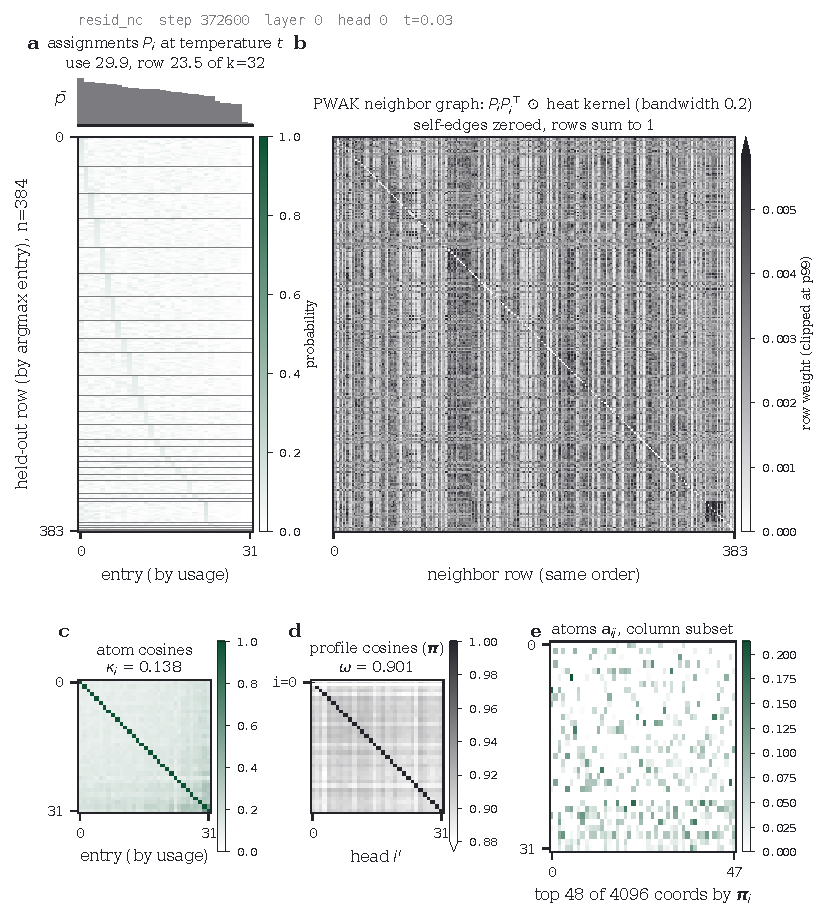
\includegraphics[width=\linewidth]{figures/fig-anatomy-softmax.pdf}
\caption[One softmax head, block by block]{\textbf{One softmax head,
	block by block.} The blocks of Figure~\ref{fig:anatomy} for head 0 of
	layer 0 of \texttt{resid\_nc} (step 372{,}600, $t{=}0.03$) on $n{=}384$
	eval-tail rows; one seed. Usage is spread across entries (use 29.9 of
	$k{=}32$), but each row is a near-uniform mixture (row 23.5; a), so
	the neighbor graph (b) is close to the heat kernel alone, with hub
	columns rather than blocks. $\kappa_i{=}0.138$, $\omega{=}0.901$, $e{=}4096$.
	As in Figure~\ref{fig:anatomy}, the model was not trained with the
	statistics that use the graph.}
\label{fig:anatomy-softmax}
\end{figure}

Trained in as hard selection, the categorical form shows row by row
(Figure~\ref{fig:assignmap}, \texttt{assignmap.py}). On both substrates
the straight-through stack's layer-0 heads put each row on one entry (row
1.0) and spread the rows over 14--30 effective entries (use), and rows
that share a label tend to share entries: most Cebuano rows sit on one
entry of each of the three SONAR heads shown, and most GPT-2 newline and
space tokens on one entry per head. An SAE on the same rows spreads each
over 25--29 effective latents of its $k_{\mathrm{SAE}}{=}32$ active and the
shown rows over 1{,}066--1{,}533; a label shows there as a set of
co-firing latents (GPT-2's newlines), not as one.

\begin{figure}[tp]
\centering
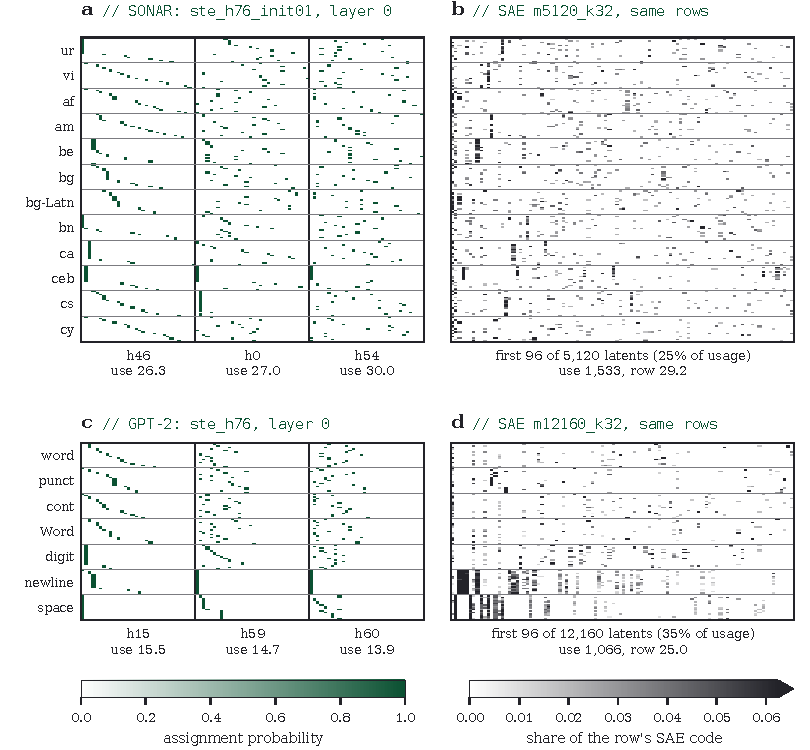
\includegraphics[width=\linewidth]{figures/fig-assignmap.pdf}
\caption[Hard codes against SAE codes, row by row]{\textbf{Hard codes
	against SAE codes, row by row.} Layer-0 assignments of the
	straight-through stacks on eval-tail rows, 24 per label value:
	(a) SONAR \texttt{ste\_h76\_init01} by language, (c) GPT-2
	\texttt{ste\_h76} by token class, for the three heads whose partitions
	carry the most NMI with the label above its shuffled null. Entries are
	sorted by usage, rows grouped by label and ordered by their winning
	entries; each head's use is under it, and its row is 1.0. (b, d) The
	same rows in the same order against an SAE trained on the same cache
	(\texttt{m5120\_k32}, \texttt{m12160\_k32}), each cell a latent's share
	of the row's code, for the 96 latents most used on these rows; the
	whole code's use and row are under it. One seed per model.}
\label{fig:assignmap}
\end{figure}

\subsection{Semantic coherence in detail}
\label{sec:coherence}

Under the whitened metric the training objective optimizes, the
Ontologizer's mean $\zeta_{\cos}$ is $-24.4$ ($-17.6$ raw; the fraction of
heads below $-2$ is unchanged at 0.96), the single-layer soft variant's
$-14.7$ (unchanged) and the hard variant's $+179.3$ ($+161.3$ raw).

Two heads of the reference softmax model cluster instead of contrasting:
layer 2's head 25 ($\zeta_{\cos}{=}{+}346$) and layer 3's head 28
(${+}280$), with the next candidates in the partially frozen layer 4.
Their sampled entries also decode to generic text, which suggests partial
head collapse (entries that never differentiated) rather than semantic
coherence; they have not been inspected further.

The description-text view of coherence is uninformative on plain
summaries, which are generic for about 77\% of entries and 49\% of
$k_{\mathrm{SAE}}{=}32$ latents and so inflate the permutation null
(Ontologizer heads $\zeta{=}{+}0.14$). On the contrastive descriptions it
acquires signal. Within-head description similarity clears the
head-membership permutation null for Ontologizer heads
($\zeta{=}{+}2.03$, 155 within-head pairs), is marginal for the
single-layer hard variant (${+}1.55$, 62 pairs), and is weaker still for
the single-layer soft variant (${+}1.09$, 217 pairs). Against the geometry, this is the pattern
that alternative values of one shared dimension predict: Ontologizer
entries' decode directions repel while their described contents weakly
cohere. It is also the first measure to separate the Ontologizer from its
single-layer soft rival, though only suggestively at this coverage (one
global $\zeta$ per model over the campaign's sampled features).

\subsection{Heads as communities of their input}
\label{sec:modularity}

A head partitions the samples it reads. Whether the partition is a
community structure of that input, with more affinity inside its cells
than a degree-preserving null graph puts there, is soft modularity
(Eq.~\eqref{eq:modularity}), compared with size-matched regroupings of the
same entries (Figure~\ref{fig:modularity}). The softmax Ontologizer is
\texttt{bl\_ctl\_full}; the SAEs are the Matryoshka rungs
\texttt{m5120\_g160top1\_p5} (trained heads) and \texttt{m5120\_k32\_p5}
(discovered groups) and the flat \texttt{m5120\_g160top1} and
\texttt{m5120\_k32}.

On the input itself nothing is a community: the Ontologizer's layer 0 is
1.25 times its null and every SAE 0.76--1.06. On each layer's own input
the Ontologizer's layers 1--4 are 2.1--2.9 times as modular as
regroupings of their entries. A Matryoshka SAE scored on matched
prefix-residual graphs is not, whether its heads are trained (0.96--1.06)
or discovered (0.88--1.03 in the blocks they cover). So the structure is
not a property of residual graphs, nor of trained heads in a
coarse-to-fine dictionary. What differs is that an Ontologizer layer
classifies the residual it is scored on, while a Matryoshka block is
encoded from the input and only trained to reconstruct that residual. Raw
modularity rises with depth in real and null alike (layer 4: 0.218
against 0.105), as assignments sharpen and the residual graphs cluster,
which is why the ratio is the comparable number. Low values on the input
are what a factorial code predicts: a head that encodes one of many
independent factors cuts across the input's neighborhoods, since
neighbors share most factors and not necessarily this one. One checkpoint
per model.

\begin{figure}[tp]
\centering
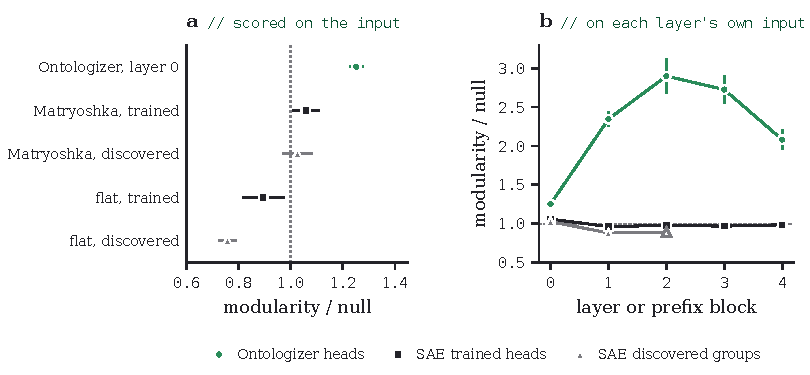
\includegraphics[width=\linewidth]{figures/fig-modularity.pdf}
\caption[Head partitions as communities of their input]{\textbf{Ontologizer
	heads are communities of the residual they classify; SAE heads and
	groups are not.} Soft modularity over its size-matched null
	(\texttt{headstruct.py --modularity}, Eq.~\eqref{eq:modularity}); bars
	are $\pm2$ null standard deviations. (a) Every model scored on the input
	itself: the softmax Ontologizer's layer 0, block 0 of the two Matryoshka
	SAEs (scored on $\mathbf{x}-\mathbf{b}_{\mathrm{dec}}$, the SAE
	encoder's input), and the two flat SAEs. (b) By depth, each layer or
	prefix block on the graph of its own input. Hollow: a block whose groups
	cover under 10\% of samples. The discovered groups' blocks 3 and 4 are
	not drawn: block 3's null is within two of its standard deviations of 0
	(3\% coverage), and block 4 holds one group, which its null reproduces
	exactly. One checkpoint per model.}
\label{fig:modularity}
\end{figure}

\subsection{Feature reliability}

Seed stability (\texttt{k32} vs.\ \texttt{k32\_s43}; identical
architecture and data, $\fvu$ 0.4994 vs.\ 0.4967): matched-feature
fractions are \textbf{0.31 / 0.24 / 0.15 / 0.03} at
$\tau{=}0.3/0.5/0.7/0.9$. Roughly three quarters of individual features
are not reproducible across initializations at moderate containment.
Cross-width splitting (\texttt{k32} $\to$ \texttt{m11264\_k32}): 190 of
5114 live parents split at $\tau{=}0.7$ (median 3 children; union
coverage 0.37; child overlap 0.42), with 441 geometric twins and a
heavy nearest-neighbor decoder-cosine tail (p50 0.234 vs.\ random
0.119): splitting is real but is not the dominant organization; topical
co-firing is. For a steering generator the unit that must reproduce is
the head's partition rather than the individual feature vector;
Section~\ref{sec:seeds} measures that on the hard-code Ontologizer and
finds it reproduces far \emph{worse} than SAE features do.

\subsection{Text-space fidelity (collateral ceiling)}
\label{sec:textfid}

\begin{table}[htbp]\centering\small
\begin{tabular}{@{}lrrr@{}}
\toprule
model & chrF & exact & NLL (ceiling 1.560, floor 3.999) \\
\midrule
corpus-mean floor & 0.176 & 0 & 3.999 \\
k32 tier (incl.\ p5, m11264) & 0.23 & 0.00 & 3.16--3.18 \\
k32\_bl          & 0.204 & 0.00 & 3.365 \\
k160 / g160top1  & 0.27--0.28 & 0.00 & 2.41--2.43 \\
onto soft        & 0.552 & 0.070 & 1.585 (gap 0.025) \\
g160softmax      & 0.591 & 0.094 & 1.568 (gap 0.008) \\
k5120            & 0.841 & 0.562 & 1.560 (gap 0.000) \\
\bottomrule
\end{tabular}
\caption{Downstream text fidelity, 512 tail rows, forced English decodes.
The NLL ceiling is the same for every model, the original's decode
scored under the original.}
\end{table}

The FVU--text mapping is sharply nonlinear: $\fvu \approx 0.5$ decodes to
same-topic-different-facts text barely above the generic floor, while the
Ontologizer's soft code and \texttt{g160softmax} are near the likelihood
ceiling --- almost all decodable content survives. Across the eleven
Ontologizer runs with both numbers (the selection sweep and the
straight-through arms; Table~\ref{tab:steerfid}), ``loss recovered'' is a
monotone function of $\fvu$ (rank correlation $-1$), so text
fidelity is a check that the whitened objective transports to text, not
an independent axis --- and it does. This matters doubly under the
steering frame: a steering primitive that routes through a code which
cannot preserve text (the entire $k_{\mathrm{SAE}}{\leq}160$ sparse tier) starts from
$\sim$0.75 collateral before any intervention, whereas the dense-mixture
classifier codes start near zero.

\subsection{Concept (language) localization}
\label{sec:langlocal}

\begin{table}[htbp]\centering\small\setlength{\tabcolsep}{4pt}
\begin{tabular}{@{}lrrrrrr@{}}
\toprule
& \multicolumn{3}{c}{86 languages} & \multicolumn{3}{c}{five languages, F1@1} \\
\cmidrule(lr){2-4}\cmidrule(l){5-7}
model & F1@1 & F1@4 & F1@16 & own tags & \stackhead[r]{it pt\\nl ja} & \stackhead[r]{ca ro\\sv ko} \\
\midrule
k160             & 0.119 & \textbf{0.393} & \textbf{0.473} & 0.684 & 0.841 & 0.841 \\
k32 ($m{=}5120$) & 0.089 & 0.347 & 0.465 & 0.624 & 0.868 & 0.876 \\
m11264\_k32      & 0.078 & 0.364 & 0.471 & 0.551 & 0.860 & 0.871 \\
k32\_bl          & 0.084 & 0.228 & 0.368 & 0.695 & 0.840 & 0.786 \\
k32\_p5          & 0.061 & 0.322 & 0.456 & 0.625 & 0.862 & 0.870 \\
g160top1         & 0.066 & 0.207 & 0.302 & 0.592 & 0.542 & 0.700 \\
g160softmax      & 0.067 & 0.162 & 0.328 & 0.432 & 0.437 & 0.433 \\
k5120            & 0.064 & 0.130 & 0.237 & 0.439 & 0.448 & 0.447 \\
softmax Ontologizer (entries) & 0.022 & 0.022 & 0.135 & 0.333 & 0.333 & 0.333 \\
hard-code stack (entries) & \textbf{0.121} & 0.153 & 0.362 & 0.685 & 0.804 & 0.806 \\
hard-code flat (entries) & 0.120 & 0.141 & 0.319 & 0.609 & 0.798 & 0.703 \\
\bottomrule
\end{tabular}
\caption{Language localization (\texttt{langprobe.py}): one-vs-rest F1
of the single best latent and of logistic probes on the best 4 and 16,
on held-out tail rows. Left, over all 86 languages, where always-match
scores 0.023 and a dense probe on the embedding 0.676. Right, single-latent
macro F1 within three five-language populations, where always-match
scores 0.333: English, French, Spanish, German and Chinese, the languages
encoded under their own SONAR tags (Appendix~\ref{app:data}), and two
populations of the same shape encoded under the English tag. The softmax
Ontologizer is \texttt{resid\_nc}, the hard codes
\texttt{ste\_h76\_init01} and \texttt{ste\_l1\_h380\_i01}.}
\label{tab:langlocal}
\end{table}

Language remains distributed in every model (best single-latent macro-F1
0.121 against a dense ceiling of 0.676; script-distinctive languages such
as Chinese reach $\sim$0.98 from one latent, same-script families smear;
Table~\ref{tab:langlocal}). The softmax Ontologizer's entry probabilities
localize nothing: at one and four entries their F1 is the always-match
floor. The hard codes' entries, which are their assignments, localize at
one entry as well as the best SAE (0.121 and 0.120 against 0.119), though
less at 4 and 16. Read on SAE terms the soft code's floor is an
indictment; read on classifier terms it is expected: a soft head encodes
a factor in its \emph{assignment}, not in any single entry's probability, and partition-level
analysis of \texttt{resid\_nc} found layer-1 heads whose partitions carry
script/family mutual information, one of which ((L1,h8,k17)) was causally
verified to force Burmese output. The partition-level instrument
(\texttt{headlang.py}) was later run on a config-matched softmax
reference and on the hard-code arms (Section~\ref{sec:lang}): the softmax
reference's best head reaches a null-corrected NMI of only $0.043$, a
quarter of the hard code's. Language factors are carried weakly and
across many heads' partitions, not by a few: in both hard-code seeds the
76 most language-informative of the 380 heads are exactly the 76 layer-0
heads (\texttt{headlang.py}), the best of them reaching about a fifth of
the attainable NMI, every deeper head carries less than any of them, and
without the top 32 the rest of the code still reads most of what they do
(Appendix~\ref{sec:langdetail}).

\paragraph{What the English tag does to localization.} Most of the
cache was encoded under SONAR's English source tag
(Appendix~\ref{app:data}), and the tag shapes this table. Each $\topk$
SAE has one latent that fires on French, Spanish and German, the three
Latin-script languages encoded under their own tags, and so separates
them from the English-tagged rest without separating them from each
other: it gives each F1@1 near 0.49, against 0.03--0.15 for Italian,
Portuguese, Dutch, Catalan, Romanian and Swedish. Restricted to the
correctly tagged languages, French and German get no latent or entry of
their own in any model (best F1@1 0.39--0.50 against the 0.33 floor),
while English (0.64--0.96) and Chinese (0.86--0.997 in the sparse and
hard codes) do. Populations of the same shape under the English tag
localize at macro F1@1 0.70--0.88 against 0.55--0.70 for the correctly
tagged one in every model but \texttt{g160top1} and the dense codes,
although a dense probe separates the correctly tagged five at least as
well (0.95--1.00 against 0.92--0.98): each English-tagged Latin-script
language carries a signature of its own. So most single-latent
localization of Latin-script languages here is the tag's signature, not
the language's. Whether a dictionary trained on correctly tagged
embeddings would give those languages a latent each is untested.

Entry-level enrichment asks the same question cell by cell
(Figure~\ref{fig:enrich}, \texttt{enrich.py}). In \texttt{resid\_nc},
3{,}698 of 226{,}763 tested (entry, language) cells are significant at FDR
0.05, and the label structure is a layer-0 property: the best head's NMI
above its shuffled null is 0.050 at layer 0 and 0.006, 0.003, 0.002 and
0.001 above it. GPT-2's hard code has the same depth profile for token
class (0.149 at layer 0, at most 0.029 above) and for position (0.105,
then at most 0.011), with 11{,}777 of 53{,}412 (entry, token class) cells
significant.

\begin{figure}[tp]
\centering
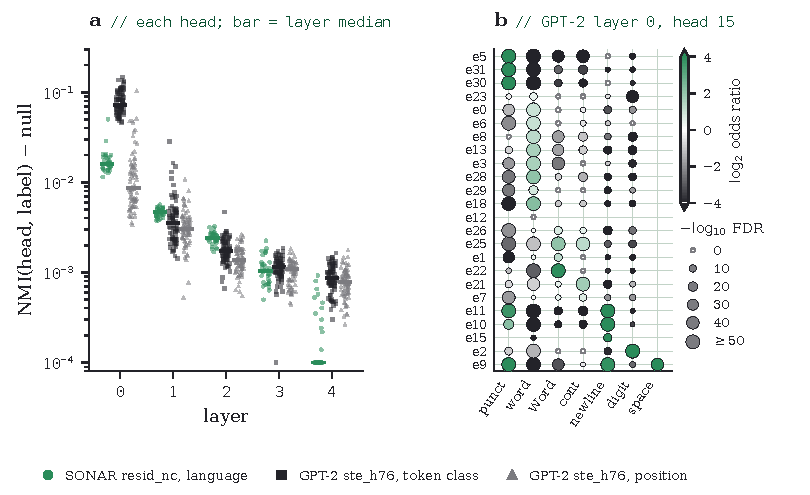
\includegraphics[width=\linewidth]{figures/fig-enrich.pdf}
\caption[Label structure by layer]{\textbf{Label structure lives in
	layer 0.} (a) NMI between each head's winning entry and a label on the
	eval tail, less its mean over five label-shuffled draws, one point per
	head (values at or below that mean drawn at $10^{-4}$) and a bar at the
	layer median: \texttt{resid\_nc} against language, GPT-2
	\texttt{ste\_h76} against token class and position. (b) The GPT-2
	layer-0 head with the most token-class NMI (head 15), each entry
	against each class: colour the Haldane-corrected $\log_2$ odds ratio,
	area $-\log_{10}$ FDR (capped at 50), filled where FDR $<0.05$;
	entries grouped by the class they are most enriched for. One seed per
	model.}
\label{fig:enrich}
\end{figure}

\subsection{Shrinkage decomposition}

$\topk$ SAEs have small magnitude error (share of raw $\fvu$ removed by
support-frozen least squares: 2.2--2.4\% for k32 variants, 8.5\% for
k160, 0.6\% bilinear, 1.9\% p5); \texttt{g160top1} is essentially
perfectly calibrated (0.3\%) --- its reconstruction deficit is pure
selection. For the Ontologizer's truncated deviation codes the refit
removes 16\% at $\nu{=}1$ and 33\% at $\nu{=}2$, about the share any
$\lvert\mathcal{S}\rvert$ free coefficients would remove from a residual
spread evenly over the whitened coordinates ($\lvert\mathcal{S}\rvert/d$
= 160/1024 and 320/1024 for \texttt{resid\_nc}'s $5\times32$ heads).
A support drawn at random, at the same size per sample, removes more:
19\% and 36\% for the Ontologizer ($\nu$ random entries per head), and
20\%, 13\% and 4.6\% for k160, \texttt{g160top1} and k32, against their
own 8.5\%, 0.3\% and 2.2\% (\texttt{refit.py}). No code's own support
removes more than chance, so nothing here shows the pin-and-renormalize
convention mis-scaling what it keeps (supports of $\geq d$ coefficients
are excluded as underdetermined). Separately, the
gap between non-adaptive truncation (freeze soft $P$, truncate, decode
linearly) and in-forward truncation (later layers reclassify against the
truncated prefix residual) is large --- $0.268$ vs.\ $0.094$ at $\nu{=}8$:
downstream layer compensation is worth $\sim$3$\times$ under truncation.
This was the first quantified reconstruction credit for the residual
stack (Section~\ref{sec:depth} measures a larger one), and it is
steering-relevant: the stack actively re-routes around code edits, which
cuts both ways --- robustness to small interventions, and, as
Section~\ref{sec:entangle} shows, widespread collateral.

\subsection{Steering through the text round trip}
\label{sec:steertext}

Across the Ontologizer selection sweep, the straight-through arm and the
$k_{\mathrm{SAE}}{=}32$ SAE, at 64 features per run:

\begin{table}[htbp]\centering\small\setlength{\tabcolsep}{4pt}
\begin{tabular}{@{}lrrrrrrrr@{}}
\toprule
run & $\fvu$ & chrF & loss rec. & net @0.25 & @0.5 & @1.0 & hit @1.0 & rand.\ hit \\
\midrule
top8          & 0.0370 & 0.416 & 0.941 & 0.203 & 0.404 & \textbf{0.652} & 0.734 & 0.359 \\
top2          & 0.3516 & 0.246 & 0.521 & 0.072 & 0.277 & 0.509 & 0.578 & 0.109 \\
top16         & 0.0052 & 0.557 & 0.987 & 0.027 & 0.110 & 0.363 & 0.381 & 0.156 \\
top4\_shm     & 0.0761 & 0.375 & 0.892 & 0.112 & 0.140 & 0.248 & 0.242 & 0.062 \\
softmax\_shm  & 0.0007 & 0.706 & 0.997 & 0.058 & 0.128 & 0.242 & 0.211 & 0.094 \\
top2\_shm     & 0.1911 & 0.301 & 0.742 & 0.018 & 0.071 & 0.196 & 0.150 & 0.016 \\
top8\_shm     & 0.0287 & 0.437 & 0.954 & $-0.015$ & 0.074 & 0.176 & 0.330 & 0.094 \\
top1          & 0.7190 & 0.170 & 0.126 & 0.047 & 0.104 & 0.064 & 0.102 & 0.109 \\
\texttt{ste\_h76} & 0.2293 & 0.295 & 0.695 & 0.033 & 0.045 & $-0.020$ & 0.055 & 0.125 \\
\midrule
SAE \texttt{k32} & 0.4994 & 0.228 & 0.345 & 0.048 & 0.187 & 0.402 & 0.260 & 0.016 \\
\bottomrule
\end{tabular}
\caption{Text fidelity and text-cycle steering (\texttt{steerfid.py},
\texttt{--n-features 64}) across selection rules, and the
$k_{\mathrm{SAE}}{=}32$ SAE under the same protocol. Net effect is feature
effect minus the random-direction control. A further run
(\texttt{topk4\_rev}, $\fvu$ 0.164) reads net 0.636 at 1.0.}
\label{tab:steerfid}
\end{table}

Steerability does not track reconstruction. The best steerer is
\texttt{top8} at $\fvu$ 0.037, the most faithful model
(\texttt{softmax\_shm}) steers at about a third of its rate, and every
\texttt{\_shm} variant steers about three times worse than its twin
(\texttt{top2} 0.509 vs.\ \texttt{top2\_shm} 0.196; \texttt{top8} 0.652
vs.\ 0.176). The straight-through arm is the weakest of all: its raw
effect is flat in magnitude (0.018, 0.014, 0.027) and no larger than a
random direction's, and its hit rate (0.055) does not clear its own
random control (0.125). The SAE steers in text by the same measure (net
0.402 at 1.0, hit 0.260 against 0.016 for random).
Two cautions on this instrument. Sixteen features is too few to quote,
and even at 64 the straight-through arm's net effect changes sign with
its random control: it was negative at every magnitude at 16 features
and is $+0.033$, $+0.045$, $-0.020$ here, so its text-cycle effect is
within the instrument's noise. And the hit rate is not
comparable across hard and soft codes: under a hard code an activation
is exactly 0 or 1, so a ``hit'' demands the argmax land exactly on the
target entry, where a soft code need only cross a fractional threshold.

\paragraph{The text cycle is too weak to support conclusions.} Measured on
an \emph{unsteered} round trip (the last 512 cache rows), the cycle
keeps part of each row's content but moves it off the corpus:
$\cos\angle(\mathbf{x}, \mathrm{cycle}(\mathbf{x}))$ is $0.382$, against
$0.091$ to another row's cycle, while cycled embeddings sit at $0.160$ to
the corpus mean, where rows sit at $0.561$. What it does not keep is the
code. A head's argmax survives the round
trip on 12.9\% of rows for \texttt{ste\_h76} and 10.8\% for the softmax
model, against 3.1\% chance; for the hard code survival falls with depth,
from 36.2\% at layer 0 to 4.8\% by layer 4. A
perfect intervention could therefore be observed at most $\sim$13\% of
the time --- the same order as the hit rates the instrument reports. The
protocol makes the cycle harder than it need be: rows are 512-token
document openings, past the length at which SONAR's auto-encoding
degrades, decoded into English whatever their language, through a decoder
that small perturbations of the embedding can derail~\cite{lcmteam2024largeconceptmodelslanguage}.
Reconstruction into embedding space is fine; generation is where the
signal goes.

\section{Supplementary results: training, reproducibility and steering of the softmax Ontologizer}
\label{app:softdyn}

These results come from the project proposal's evaluation and concern the
softmax Ontologizer. Two models recur. \texttt{resid\_nc} (372{,}600 steps)
is the reference model behind the softmax tables above.
\texttt{resid\_nc\_hm} is the same configuration plus the batch
mean-entropy bonus $s_{\mathrm{KL}_m}$, trained to 4.38M steps; results
here use its final checkpoint unless stated otherwise.

\subsection{Head freezing and the mean-entropy bonus}
\label{sec:freeze}

A head is counted frozen when its top classification share is at least
$0.95$ and its churn at most $0.02$. In \texttt{resid\_nc} the top layer
(layer 4 of 0--4) begins freezing near step 190k, well after the
temperature anneal, reaches 27 of 32 heads by step 210k and 28 at its
peak, and is still frozen at the last checkpoint
(Figure~\ref{fig:freeze}). Section~\ref{sec:lastlayer} shows the same
layer to be inert once the prefix error is small, which is why the freeze
costs so little reconstruction. In \texttt{resid\_nc\_hm} the late freeze
never occurs. What remains is an early annealing transient --- 22 of 32
heads at layer 1 at step 10k, with 16, 11 and 4 of 32 at layers 2, 3 and 0
--- that recovers completely by step 30k, leaving the final checkpoint
unfrozen everywhere. \textbf{The mean-entropy bonus prevents the late
freeze.}

\begin{figure}[htbp]\centering
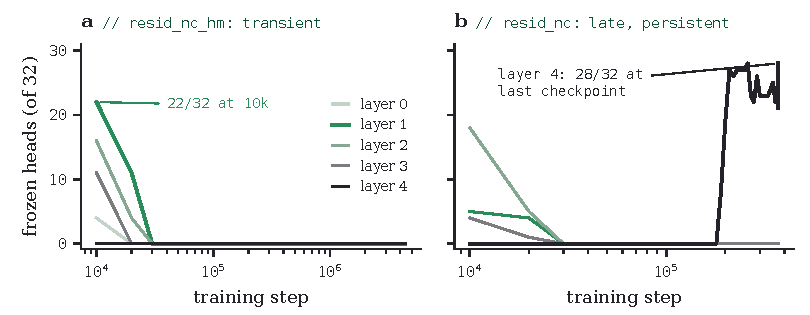
\includegraphics[width=\linewidth]{figures/fig-freeze.pdf}
\caption{Frozen heads per layer over training. (a)
\texttt{resid\_nc\_hm}, with the mean-entropy bonus, has only an early
annealing transient, peaking at 22/32 in layer 1 at step 10k and
recovering to zero everywhere by step 30k. (b) \texttt{resid\_nc}
develops a post-anneal layer-4 freeze from ${\sim}$190k that persists
through its last checkpoint.}
\label{fig:freeze}
\end{figure}

Four retrains of the \texttt{resid\_nc\_hm} configuration (372k steps
each) isolate the transient: a zero-change control and three single-knob
variants. The control reproduces it head for head (22/32 at layer 1 at step
10k, zero everywhere by 30k) and shows no late freeze. Stretching the
temperature anneal from 50k to 150k steps attenuates and spreads it (peak
14/32 at layer 1 at step 30k, clear by 50k). Raising winner dropout from
$0.1$ to $0.25$ tracks the control to within two heads at the peak, and
holding the classification-noise floor at its starting value changes
nothing (Figure~\ref{fig:variants}). The transient belongs to the
temperature schedule alone, and every retrain ends unfrozen.

\begin{figure}[htbp]\centering
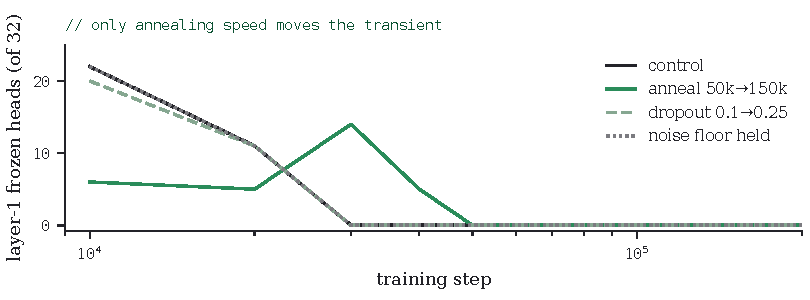
\includegraphics[width=\linewidth]{figures/fig-variants.pdf}
\caption{The early transient under the four retrains, layer-1 frozen
count. The noise-floor variant overlaps the control exactly and the
dropout variant tracks it to within two heads at the peak; only
stretching the temperature anneal moves the curve, trading peak height
for duration.}
\label{fig:variants}
\end{figure}

\paragraph{An HSIC penalty in place of the auxiliary losses.} The arms
are named after the HSIC bottleneck~\cite{ma2020hsic}, which trains each
layer without backpropagation to depend little on its input and much on
the class labels, both measured by normalized HSIC. An autoencoder's
labels are its input, which collapses the two terms into one, so neither
is used here: reconstruction stays with the whitened MSE, and the only
kernel term penalizes dependence among a layer's heads. Two arms on the
\texttt{resid\_nc\_hm} configuration, trained to 372k steps, penalize it
by the pairwise head CKA of Section~\ref{sec:hsic} under the biased
estimator~\cite{gretton2005}: one replaces the four
auxiliary terms with that penalty, the other adds it to them. Replacing
them destroys head health: a late, persistent freeze takes 77 of 160
heads by the final checkpoint, one layer entirely (layer 3, 32/32 from
step 80k), while reconstruction lands slightly behind the control
(tail-mean training MSE $3.7\times10^{-5}$ against $3.4\times10^{-5}$).
Adding the penalty to the auxiliary terms is worse on both counts: MSE
$4.4\times10^{-5}$, and 41 of 160 heads still frozen at the end, layer 3
fully frozen by 80k with only partial thaw
(Figure~\ref{fig:hsicbottleneck}). The failure is \texttt{resid\_nc}'s
late freeze rather than the transient, and it is the estimator's. The
biased floor between independent heads falls with the number of entries
a head uses and is zero for a frozen head (Section~\ref{sec:hsic}), so
the penalty can only be lowered by concentrating or freezing heads,
which puts it in direct opposition to the mean-entropy bonus. Retrained
on the current code, the replacement arm reproduces the freeze
checkpoint for checkpoint (layer 3: 6, 29 and 32 of 32 frozen at 60k, 70k
and 80k, against 7, 29 and 32) while its summed penalty falls by 80\%;
under the unbiased estimator the same arm freezes at most 5 heads, all in
layer 4, by 93k steps (one seed each). With the corrected estimator the
penalty has almost nothing to act on, and whether it could replace the
auxiliary terms over a full run is untested.

\begin{figure}[htbp]\centering
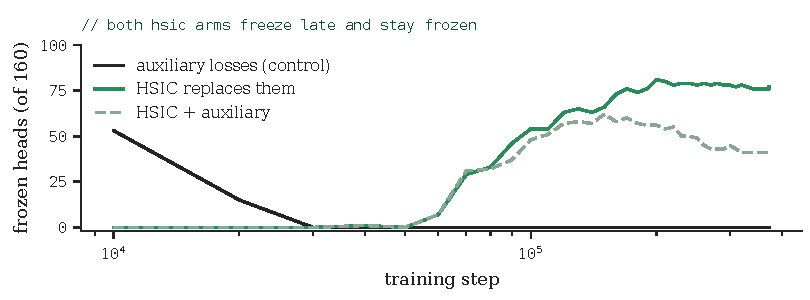
\includegraphics[width=\linewidth]{figures/fig-hsic.pdf}
\caption{Total frozen heads over training for the three loss
configurations, all on the \texttt{resid\_nc\_hm} configuration at 372k
steps. The auxiliary-loss control's freeze is the early transient and
resolves; both HSIC arms, whose head-CKA penalty uses the biased
estimator, develop the late, persistent freeze instead, and the
auxiliary terms only partially thaw it.}
\label{fig:hsicbottleneck}
\end{figure}

\subsection{Development over training}
\label{sec:devinterp}

Tracking \texttt{resid\_nc\_hm}'s full 448-checkpoint history applies the
z-score machinery of Section~\ref{sec:prelim-orth} to the refit
end-to-end direction matrix rather than to raw dictionary decode
directions. The two are not directly comparable: raw decode directions on
\texttt{resid\_nc} repel ($\zeta_{\cos}{=}{-}17.6$), while refit directions on
\texttt{resid\_nc\_hm}'s final checkpoint cohere ($\zeta_{\cos}{=}{+}72$); they differ
in both instrument and substrate, and the refit frame folds in the shared
decoder and cross-layer interactions. On that statistic the shape is rise,
peak and partial relaxation (Figure~\ref{fig:devinterp}): mean within-head
$\zeta_{\cos}$ climbs from $1.8$ at step 10k to a peak of $119$ near step 370k
(median $123$, every head above $\zeta_{\cos}{=}2$), then relaxes over the
remaining 4M steps to $72$ at the final checkpoint (median $105$, $0.79$
above $\zeta_{\cos}{=}2$). The code itself moves the other way after the annealing
transient: per-sample entropy returns to $4.5$ of a 5-bit maximum and usage
KL falls toward uniform. Relative to initialization, the consolidation is
in the geometry the classifications write, while the classifications stay
soft.

\begin{figure}[htbp]\centering
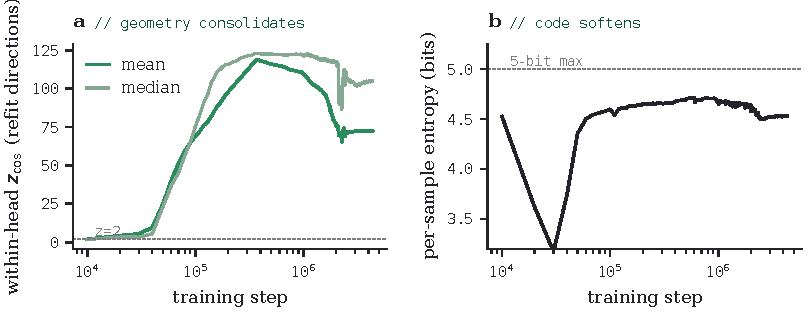
\includegraphics[width=\linewidth]{figures/fig-devinterp.pdf}
\caption{The 448-checkpoint training history of \texttt{resid\_nc\_hm}.
(a) Within-head coherence of refit end-to-end directions, z-scored
against size-matched nulls; rise, peak near step 370k, partial
relaxation. (b) Mean per-sample classification entropy returns toward
the 5-bit maximum after the annealing transient.}
\label{fig:devinterp}
\end{figure}

Entry by entry, \texttt{resid\_nc}'s dictionary settles after the anneal
(Figure~\ref{fig:entrydrift}, \texttt{entrydrift.py}). In layers 0--3 a
used entry's decoded atom has median cosine 0.40--0.51 with its final
direction at step 10k, 0.73--0.82 at 60k, just after the anneal, and
0.99--1.00 from 320k. Layer 4 starts at 0.23, stalls near 0.53 from 60k to
160k and converges only after its freeze near 190k
(Section~\ref{sec:freeze}), keeping 142 of its 1{,}024 entries. Usage
dips at the anneal's end instead: 40\% of layer 0's entries fall out of
use at 60k, and all but 7\% are back in use by the end. One seed.

\begin{figure}[tp]
\centering
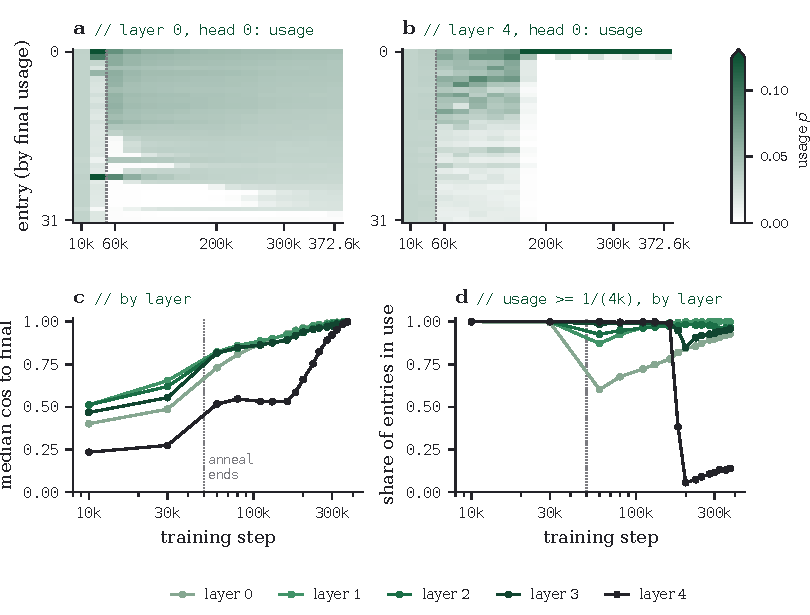
\includegraphics[width=\linewidth]{figures/fig-entrydrift.pdf}
\caption[Entry drift over training]{\textbf{Entries settle after the
	anneal.} \texttt{resid\_nc}'s 16 retained checkpoints on the eval tail.
	(a, b) Usage $\bar{p}_{ij}$ of head 0's 32 entries in layers 0 and 4,
	one column per checkpoint (not to scale in step), entries ordered by
	final usage; the dotted line marks the anneal's end. (c) Per layer, the
	median cosine between an entry's decoded atom and its final direction,
	over the entries in use at the last checkpoint. (d) Per layer, the
	share of entries in use ($\bar{p}_{ij}\geq 1/4k$). One seed.}
\label{fig:entrydrift}
\end{figure}

\subsection{Scaling: a star sweep}
\label{sec:starsweep}

Seven configurations around the shared $h{=}32$, $k{=}32$, $l{=}5$ shape,
varying one axis at a time, each trained 4 epochs (62k steps against the
retrain recipe's 372k), test whether head coherence rises with parameter
count. No measured axis delivers the rise: coherence shows no positive
relation to parameter count (Spearman $+0.14$ for mean $\zeta_{\cos}$,
$-0.54$ for the fraction above $\zeta_{\cos}{=}2$), usage imbalance grows
with size ($+0.86$), and the cleanest per-axis trend runs opposite to the
prediction, coherence falling monotonically as entries per head grow
($k{=}16/32/64$: mean $\zeta_{\cos}$ $20.2/6.3/3.7$). The widest model ($h{=}64$) has not converged at
this budget (tail MSE $20\times$ the others), so its collapse is not
evidence (Figure~\ref{fig:scaling}). Seven points at short training are
weak evidence either way; full-length retrains are the missing control.

\begin{figure}[htbp]\centering
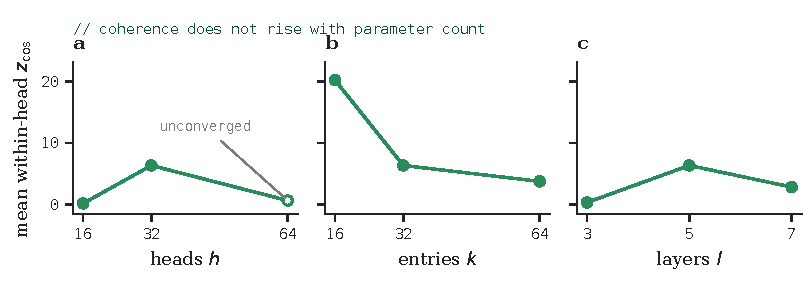
\includegraphics[width=\linewidth]{figures/fig-scaling.pdf}
\caption{Head coherence against each parameter axis of the star sweep:
heads (a), entries (b) and layers (c), all runs at 4 epochs (62k steps). No axis delivers the predicted rise;
the entries axis falls monotonically. The open marker in (a) is the unconverged
$h{=}64$ run.}
\label{fig:scaling}
\end{figure}

\subsection{Seed stability of soft partitions}
\label{sec:softseed}

A second run of the \texttt{resid\_nc\_hm} configuration from a different
seed, compared at matched training (370k steps on both sides), matches
essentially nothing (Figure~\ref{fig:softseed}): no head pair and at most
$0.3\%$ of atoms clear a $0.3$ cosine threshold on dictionary geometry,
and activation-frame containment over a shared evaluation batch is at most
$0.001$ at any threshold, against $0.31/0.24/0.15/0.03$ for the k32 SAE and
its seed replica across the four thresholds ($0.3$--$0.9$). The metric has
headroom: the same run against itself $2{,}600$ steps apart scores $1.000$
on geometry at every threshold and $0.65$ at the loosest activation
threshold ($0.20$ at the strictest). At matched training the softmax
Ontologizer's partitions are less reproducible across seeds than SAE
latents, the same verdict Section~\ref{sec:seeds} reaches for the
straight-through arm with partition and contribution measures. A replica
carried to the full 4.4M steps is the remaining control.

\begin{figure}[htbp]\centering
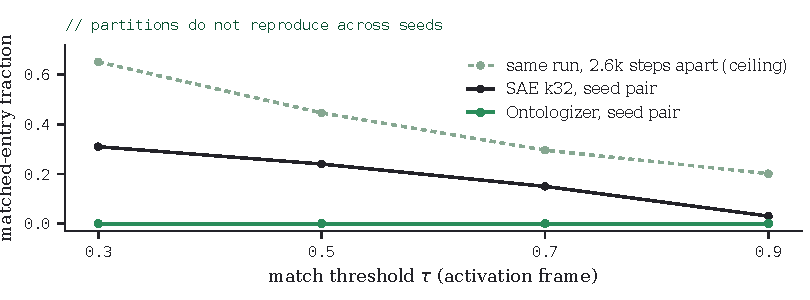
\includegraphics[width=\linewidth]{figures/fig-seed.pdf}
\caption{Cross-seed matched-entry fraction on the activation frame by
threshold. The same-run pair bounds what the metric can detect ($0.65$
at $\tau{=}0.3$); the k32 SAE pair reproduces partially; the softmax
Ontologizer's partitions reproduce not at all.}
\label{fig:softseed}
\end{figure}

\subsection{Steering against supervised baselines}
\label{sec:steeroverlay}

A matched-budget overlay on \texttt{resid\_nc\_hm} at step 4{,}380{,}000,
the last checkpoint kept, compares forced classifications against
difference-of-means and linear-probe directions on language steering,
with a random-direction floor (Table~\ref{tab:steer-overlay}). Each arm
wins its own effect frame, as expected. On the shared difference-of-means
frame, forcing a classification moves decodes along the target direction
$0.64\times$ as far as supervised steering does, and $4.2\times$ as far as
probe directions. No arm reliably reaches the target language: the
median hit rate is $0.06$ for the difference of means and 0 for the other
arms. Every arm's collateral,
supervised steering included, sits at the random-direction floor
($0.70$--$0.78$), the same floor the text round trip shows for SAE
steering (Section~\ref{sec:steertext}). On naturalness the arms are so
far indistinguishable (Figure~\ref{fig:naturalness}): chrF against
unsteered decodes falls from ${\sim}0.37$ at magnitude $0.25$ to
${\sim}0.15$ at $1.0$ for the difference-of-means and
forced-classification arms, with probe and random decaying in parallel
from $0.38$--$0.40$ to $0.19$--$0.20$. A blinded human-rating sheet (120
items) is prepared but unscored.

\begin{table}[htbp]\centering\small
\begin{tabular}{@{}lrrrr@{}}
\toprule
arm & effect (native) & effect (dm frame) & hit rate & collateral \\
\midrule
difference of means    & 0.474 & 0.474 & 0.062 & 0.752 \\
classification forcing & 0.399 & 0.302 & 0.000 & 0.776 \\
linear probe           & 0.294 & 0.072 & 0.000 & 0.701 \\
random direction       & ---   & ---   & ---   & 0.705 \\
\bottomrule
\end{tabular}
\caption{Language steering under matched intervention budgets on
\texttt{resid\_nc\_hm} at step 4{,}380{,}000; medians over 24
language--magnitude conditions per arm. Effect is displacement along the arm's
own direction (native) and along the shared difference-of-means direction
(dm frame); hit rate is the fraction of steered decodes reaching the
median projection of genuine target-language rows on the shared frame;
collateral is content change on unrelated dimensions.}
\label{tab:steer-overlay}
\end{table}

\begin{figure}[htbp]\centering
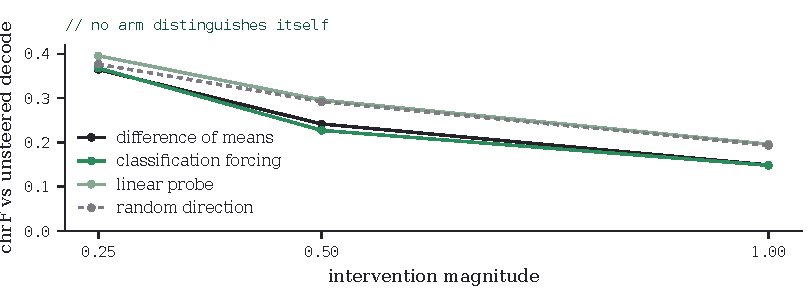
\includegraphics[width=\linewidth]{figures/fig-naturalness.pdf}
\caption{chrF between steered and unsteered decodes by intervention
magnitude. All four arms, the random direction included, damage the
decode at nearly the same rate; no arm buys naturalness at matched
magnitude.}
\label{fig:naturalness}
\end{figure}

\paragraph{A classification as a training objective.} A policy over
steering directions on frozen \texttt{resid\_nc\_hm}, rewarded by one
classification's quantile-normalized score at a matched intervention
budget, converges cleanly in the differentiable in-embedding tier,
saturating within roughly 40 steps (Figure~\ref{fig:rl}). That tier trains
by gradient ascent through the frozen model, as a ceiling for the
decode-cycle tier, whose reward passes through text generation and so
needs REINFORCE~\cite{williams1992}; the curve does not show how fast
REINFORCE would learn. Its collateral cannot move far either. The policy
adds a direction to the unit-norm embedding at a fixed length of 0.5 and
renormalizes, which caps the collateral at 0.134; it falls from 0.105 to
0.083 as the policy tilts its direction toward the row and so shortens
its effective step. The policy's step is the residual form that
latent-space steering of diffusion policies outperforms by acting on the
generator's input instead~\cite{wagenmaker2025}, and a direction
optimized against a classifier can realize its target through directions
the data never vary along~\cite{makelov2023}. Neither the decode-cycle
tier nor a convergence race against paired steering has been run.

\begin{figure}[htbp]\centering
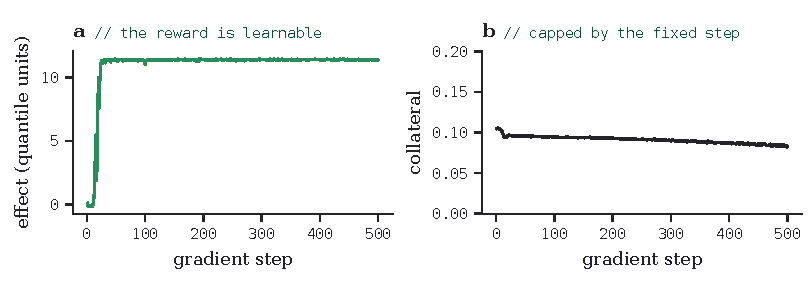
\includegraphics[width=\linewidth]{figures/fig-rl.pdf}
\caption{A steering policy trained by gradient ascent on a single frozen
classification's quantile-normalized score, in-embedding tier. The policy
saturates the reward within roughly 40 steps (a); collateral, capped at
0.134 by the fixed step length, falls from 0.105 to 0.083 (b).}
\label{fig:rl}
\end{figure}

\subsection{Head-level autointerp}
\label{sec:headautointerp}

The per-latent lenses of the description-specificity results mis-measure
classifier codes, whose content lives in partitions, so a head-level pass
over \texttt{resid\_nc} (step 372{,}600) tests the claim directly; its
frozen top layer (Section~\ref{sec:freeze}) is a caveat for any layer-4
heads in the sample. Descriptions decoded from dictionary parameters fail
at the partition level as they do per latent (median self accuracy
$0.000$, as is the null's). Activation-grounded head descriptions do no
better than a null pairing at this sample size (20 heads per condition,
median accuracy $0.083$ against $0.125$, where guessing one value per head
scores about $0.11$), and a head's detection accuracy is uncorrelated
with the mean describability of its latents (Spearman $+0.12$ over 30
head--lens pairs; $+0.25$ under activations and $+0.05$ under
parameters, 15 heads each, $p{=}0.37$ and $0.86$). The two lenses disagree and neither shows
above-chance head-level signal, so the mis-measurement argument predicts
an advantage this sample does not deliver.

\paragraph{Describability against density.} Across the six runs of the
description-specificity table, the correlation between log nominal
density and activation-description F1 is $-0.894$, so density alone
carries about 80\% of the variance. Fitting contrastive-description F1
linearly in log firing rate on the four \texttt{sae.py} runs with a
nonzero firing rate (slope $-0.069$, correlation $-0.766$), and holding the
Ontologizer out, predicts 0.421 against an actual 0.392, a residual of
$-1.8$ standard errors: the Ontologizer sits on the trend, and
\texttt{g160top1} lies 0.120 above it. The fit is thin. It rests on four
runs and a weak correlation, it excludes \texttt{g160softmax}, whose
thresholded firing rate is exactly zero, and the $2/k$ threshold is not
monotone in true density.

\paragraph{Describability against language.} Counting the distinct
languages among each feature's 15 judged rows (\texttt{autointerp.py
language}; Table~\ref{tab:autointerp-lang}) separates the sparse codes
from the dense ones before any description is read. Within each sparse
run F1 falls as the count grows (Spearman $-0.47$ to $-0.67$, activation
descriptions), and within the dense runs it does not ($-0.06$ to
$+0.03$). For \texttt{k32} and \texttt{g160top1} the modal language makes
up 28--30\% of the held-out positives the judge sees, against about 1\%
of the negatives and of the contrastive background. Refitted on the
features spanning 13--15 languages, the contrastive trend in log firing
rate puts \texttt{g160top1} 0.018 above it rather than 0.120, and the
Ontologizer 0.049 above it rather than 0.029 below. Per feature, purity
explains a fifth of the variance in F1 (0.20 for activation descriptions,
0.22 for contrastive ones) and log firing rate 1--4\%. Holding language
fixed needs matched rows on both sides, which \texttt{autointerp.py
match} draws for a contrastive background (\texttt{describe --mode
cacts\_lang}) and for the negatives (\texttt{score --negatives lang});
neither has been scored.

\begin{table}[htbp]\centering\small\setlength{\tabcolsep}{4pt}
\begin{tabular}{@{}lrrrrrrr@{}}
\toprule
& \multicolumn{4}{c}{features by languages spanned} & & \multicolumn{2}{c}{F1, all / 13--15 languages} \\
\cmidrule(lr){2-5}\cmidrule(l){7-8}
model & 1--3 & 4--9 & 10--12 & 13--15 & purity & \texttt{acts} & \texttt{cacts} \\
\midrule
onto (resid\_nc)   & 0  & 5  & 43 & 177 & 0.158 & 0.473 / 0.460 & 0.392 / 0.380 \\
k32                & 63 & 55 & 68 & 64  & 0.466 & 0.645 / 0.564 & 0.603 / 0.482 \\
k32\_bl            & 9  & 9  & 10 & 47  & 0.277 & 0.578 / 0.502 & 0.470 / 0.338 \\
g160top1           & 41 & 24 & 32 & 53  & 0.440 & 0.646 / 0.467 & 0.594 / 0.383 \\
g160softmax        & 0  & 5  & 72 & 179 & 0.183 & 0.449 / 0.443 & 0.364 / 0.347 \\
k5120 (dense ctrl) & 0  & 2  & 18 & 236 & 0.131 & 0.470 / 0.470 & 0.332 / 0.322 \\
\bottomrule
\end{tabular}
\caption{Detection F1 of Table~\ref{tab:autointerp} by the number of
distinct languages among each feature's 15 judged rows (the 10 a
description was written from and the 5 held-out positives; 15 random rows
span 13.8). Purity is the share of the description rows in their modal
language. One seed per run.}
\label{tab:autointerp-lang}
\end{table}

\section{Supplementary results: the straight-through arm}
\label{app:ste}

\subsection{Calibration}
\label{sec:calib}

A naive port (live configuration, \texttt{select="ste"}) trains but the
classifier learns nothing. The root cause is one property: \textbf{the
argmax forward is scale-invariant, so here nothing pushed the logits up};
they sat at their initialization scale for the whole run (within-head
standard deviation $0.0015$, near the $2/(d{+}1) \approx 0.0020$ that the
fan-in initialization gives a bilinear logit on a unit-norm shape with its
constant coordinate --- the variance argument behind scaled dot-product
attention~\cite[fn.~4]{vaswani2017}, at degree two). VQ-VAE meets the same gap, an encoder scale
the code does not constrain, with a commitment loss~\cite{vandenoord2017}.
Three settings follow from it.
\emph{Logit noise must be relative}: $\sigma_K{=}0.02$ is thirteen times
the logit spread, so the argmax is chosen by noise, while $\sigma_K{=}0$
removes the only exploration and the codebook collapses;
\texttt{--noise-k batchnorm} (Eq.~\eqref{eq:noise_batchnorm}) scales
noise by the logit RMS. \emph{The surrogate temperature must track the
logit scale}: at the live floor $t{=}0.03$, spread$/t$ is 0.05 and the
surrogate is flat, so what improves is the dictionary adapting to a fixed
random partition. \emph{$s_{\mathrm{KL}_m}$ must be rescaled}: $10^{-6}$ is
calibrated against a whitened MSE of $\sim$$3\times10^{-6}$, and a hard
code trains at an MSE orders of magnitude larger, where the term is inert
and heads collapse.

\begin{center}\small
\begin{tabular}{@{}lrrrr@{}}
\toprule
$t$ & spread$/t$ & max $p$ & effective entries/head & raw FVU \\
\midrule
0.01    & 0.15  & 0.043 & 23.4 & 178 \\
0.0015  & 0.78  & 0.135 & 26.4 & 193 \\
0.0005  & 3.38  & 0.681 & 14.0 & 59.2 \\
0.00015 & 16.84 & 0.974 & 3.8  & 7.3 \\
\bottomrule
\end{tabular}
\end{center}

(4000 steps, lr $10^{-5}$, \texttt{--noise-k batchnorm --sd-k 0.3}; one
seed per arm, which ranks configurations but does not predict final
quality.) Sharpening the surrogate is what makes the classifier train at
all and improves reconstruction 25-fold, but it trades directly against
head usage, which $s_{\mathrm{KL}_m}$ exists to hold. At \texttt{sonar.py}'s
learning rate $5\times10^{-5}$ every sharp-surrogate arm collapsed
abruptly after $\sim$1700 steps; $10^{-5}$ is stable. The shipped arm is
$t{=}1.5\times10^{-4}$, lr $10^{-5}$, \texttt{--noise-k batchnorm
--sd-k 0.3}, $s_{\mathrm{KL}_m}{=}10^{-4}$, trained 24 epochs
(369{,}500 steps). The temperature is hand-matched to a logit scale
measured once, and that scale moves: over training the shipped arm's
layer-0 logits shrink 2.9-fold, so spread$/t$ falls from 13 at
initialization to 4.5, while its relative noise changes 20--29\% of
layer-0 assignments throughout (\texttt{logitscale.py}, on 2{,}048 tail
rows). Scale invariance leaves the logits free to move either way, and
the GPT-2 arms, at the naive port's settings, show the other way:
\texttt{ste\_h76}'s layer-0 logits, from a classifier without a gate,
grew 452-fold, so its absolute noise, which changed more than half of the
layer-0 assignments through 50{,}000 steps, changed about 1\% from
150{,}000 on. The concatenated seed pair's sigmoid-gated classifiers kept
their initial scale, and there the noise changed 71--90\% of layer-0
assignments at every one of 16 checkpoints scored. The principled
version normalizes logits per head or controls $t$ against a spread$/t$
setpoint.

\subsection{Capacity beyond bits, and training dynamics}
\label{sec:capacity}

\paragraph{Distance from the Gaussian reference.} Measured against the
Gaussian reference at each code's own rate, the full stack sits further
from it than one layer's prefix does. Each ratio bounds that code's
distance from the optimum at its rate from below, since the optimum for
real data may lie below the reference:

\begin{center}\small
\begin{tabular}{@{}lrrr@{}}
\toprule
code & Gaussian reference & achieved & ratio \\
\midrule
380 bits (one layer's prefix) & 0.4208 & 0.537 & 1.28$\times$ \\
1900 bits, $5\times76$ & 0.0499 & 0.1535 & 3.08$\times$ \\
1900 bits, $5\times380$, $k{=}2$ & 0.0499 & 0.1844 & 3.70$\times$ \\
\bottomrule
\end{tabular}
\end{center}

\paragraph{Bits are not the whole capacity.} At identical bits, 380
binary heads reach $0.1844$ against 76 thirty-two-way heads at $0.1535$:
bits go as $h\log_2 k$ but the codebook goes as $h\cdot k$ (3800 atoms
against 12{,}160). The binary arm also trained at half the batch size
(Table~\ref{tab:cfg-ste-sonar}), so the gap mixes the larger codebook with
a noisier gradient. A neural codec's residual quantizers point the same
way: at a fixed 80 bits per frame, eight stages of 1024 codes beat eighty
of two~\cite{zeghidour2021}. The binary arm gets within 17\% on $2.9\times$ fewer
parameters, with features that are one bit each --- the form that is
actually nameable.

\paragraph{Realized bits, and what they bound.} This paragraph follows
information theory in writing random variables in uppercase. For a hard
code and a random input $\mathbf{X}$, write $A_{\ell i}$ for the entry
head $(\ell,i)$ chooses and $\mathbf{A}$ for all of them. \emph{Realized
bits} are the summed entropy of each head's usage over the data,
\begin{equation}
	H_{\mathrm{real}} := \sum_{\ell,i} H(A_{\ell i})
	= \sum_{\ell,i} \big(\log_2 k - \mathrm{KL}(\bar{\mathbf{p}}_{\ell i} \,\Vert\, \mathrm{uniform})\big)
	\;\geq\; H(\mathbf{A}) = I(\mathbf{X}; \mathbf{A}),
	\label{eq:realized}
\end{equation}
with $\bar{\mathbf{p}}_{\ell i}$ head $(\ell,i)$'s usage distribution, its
mean assignment; summed over layers this is $h(l\log_2 k - \mathrm{KL}_m)$
in the logged statistic's terms. Because
the code is a deterministic function of the input, its joint entropy is
exactly the information it carries about the input, and subadditivity
puts the sum of marginal entropies above it, with equality only when the
heads are independent. Realized bits therefore measure how evenly each
head uses its entries, not how much the code says: two codes at the same
$H_{\mathrm{real}}$ can carry different information if their heads are redundant to
different degrees, and the joint entropy, which needs a density estimate
over $k^{lh}$ outcomes, is not measured here.

\paragraph{Training dynamics.} On the shipped arm the training-log MSE
(the deep-supervision prefix mean) is flat from step 237k while
within-head row collinearity keeps falling ($0.812 \to 0.686$, against
$\sim$0.64 for random non-negative rows). Its heads' usage collapses early
and never evens out (Figure~\ref{fig:realized-bits}): realized bits fall
to 43\% of nominal near step 6k, recover to 85\% by 20k as the
$s_{\mathrm{KL}_m}$ rescale turns the usage collapse around, and end at
90\%. At the fixed initialization every head's usage is near-uniform by
step 5k (99\% of nominal), in the stack and the flat arm alike, and stays
there. Realized bits come from the logged
$\mathrm{KL}_m$, $h(l\log_2 k - \mathrm{KL}_m)$, less its sampling floor:
$\mathrm{KL}_m$ is a plug-in estimate on one batch of 256 rows, which
reads $(k-1)/(2b\ln 2) = 0.087$ bits per layer even for perfectly
balanced usage, and on the converged fixed-init arms the logged value is
almost entirely that floor. Corrected, the endpoints match the held-out
measurement of Table~\ref{tab:init} to within a bit; the correction
assumes every entry is live, so it overstates the shipped arm by 14 bits.

\begin{figure}[tp]\centering
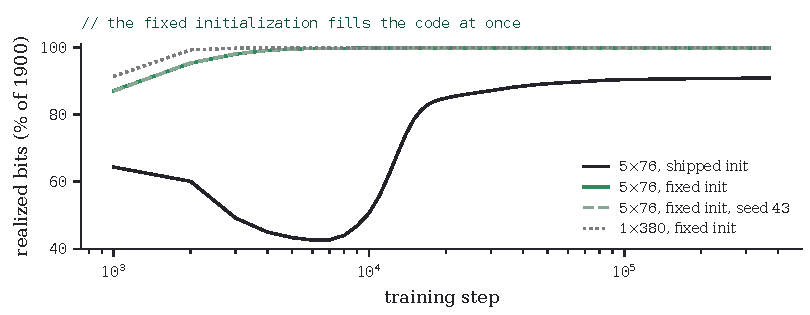
\includegraphics[width=\linewidth]{figures/fig-realized-bits.pdf}
\caption{Realized code bits over training, as a share of the nominal 1900,
from the logged $\mathrm{KL}_m$ less its one-batch sampling floor. The
shipped initialization's head usage collapses to under half before
recovering to 90\% (the curve's 91\% over-corrects heads with dead
entries); at the fixed initialization every head in the stack and the
flat arm reaches near-uniform usage within 5k steps. An upper bound on the
information carried, not a measure of it (Eq.~\eqref{eq:realized}).}
\label{fig:realized-bits}
\end{figure}

\subsection{Operational rate: every code quantized}
\label{sec:quantrate}

Index bits and coefficient counts cannot rank a code that sends
coefficients against one that does not. With everything each code sends
quantized and entropy-coded (Eq.~\eqref{eq:quantrate}), every code becomes
a curve on one rate axis (Figure~\ref{fig:quantrate}). At the stack's
1900 bits:

\begin{center}\small\setlength{\tabcolsep}{4pt}
\begin{tabular}{@{}lrrrr@{}}
\toprule
code & \stackhead[r]{$\fvu$\\unquantized} & \stackhead[r]{1900 bits,\\entropy-coded} & \stackhead[r]{1900 bits,\\fixed supports} & \stackhead[r]{1900 bits\\on every row} \\
\midrule
straight-through, $5\times76$ & 0.1536 & \textbf{0.155} & \textbf{0.158} & 0.158 \\
L1 SAE, $s_{\mathrm{L1}}{=}3\times10^{-6}$ & 0.0052 & \textbf{0.129} & 0.182 & \textbf{0.152} \\
softmax Ontologizer & 0.0054 & 0.145 & 0.239 & --- \\
L1 SAE, $s_{\mathrm{L1}}{=}10^{-5}$ & 0.048 & 0.175 & 0.180 & 0.200 \\
L1 SAE, $s_{\mathrm{L1}}{=}3\times10^{-5}$ & 0.219 & 0.242 & 0.243 & 0.250 \\
$\topk$ SAE, $k_{\mathrm{SAE}}{=}5120$ & 0.0001 & 0.243 & --- & 0.281 \\
$\topk$ SAE, $k_{\mathrm{SAE}}{=}160$ & 0.258 & 0.259 & 0.259 & 0.258 \\
\texttt{g160top1} & 0.274 & 0.274 & 0.274 & 0.274 \\
\texttt{g160softmax} & 0.0044 & 0.372 & 0.364 & 0.454 \\
\bottomrule
\end{tabular}
\end{center}

Entropy-coded, a coarsely quantized L1 SAE beats the stack at the stack's
own rate averaged over rows: 0.129 against 0.155, and the stack's
pure-code 0.158 at 1675 bits. It sends about 440 of its roughly 1600
coefficients, at about 4.3 bits each with their support. L1 latents fire
unevenly, so the support codes about 20\% below its fixed-length cost,
while the stack uses its entries almost uniformly (1895 of 1900 bits;
Table~\ref{tab:init}) and has nothing to save. Its rows also differ: the
number of coefficients a row sends varies, so near 1900 bits on average
its rows take 1406 to 2399 bits (5th to 95th percentile). The stack's
pure code takes exactly 1900 on every row at fixed length, and
entropy-coded its rows differ only by the few bits its entries'
frequencies set. Held to the budget on every row, each row at the
least-error step that fits once about 6 bits name the step, the L1 SAE
reaches 0.152, level with the stack, and needs 1853 bits per row to
reach the stack's 0.158; codes of fixed support do not move, and the
other variable ones lose more (the dense $\topk$ SAE 0.243 to 0.281,
\texttt{g160softmax} 0.372 to 0.454). Average rate is the usual measure
for compression, and a per-row budget the fairer one for a fixed set of
variables per input. With supports at their fixed-length cost the stack
leads every SAE (0.158 against 0.180). The $\topk$ SAE flattens at its
unquantized error from about 1900 bits on, consistent with its
least-squares floor of 0.236, and is already at 0.275 at 1121 bits, so
its coefficients carry little beyond which latents fire; the single-layer
hard variant behaves the same way. The softmax model's own code,
quantized around its mean assignment, reaches 0.145, and the same on rows
no model trained on. The stack's gains cost 4.8 bits at a step of two standard deviations
(taking it from 0.158 to 0.155) and 28 bits to recover the unquantized
0.1536. No code was trained for this codec: uniform usage is the most
expensive kind to entropy-code, and no SAE was trained with quantized
coefficients, so the curves rank these models, not their architectures.

\begin{figure}[tp]\centering
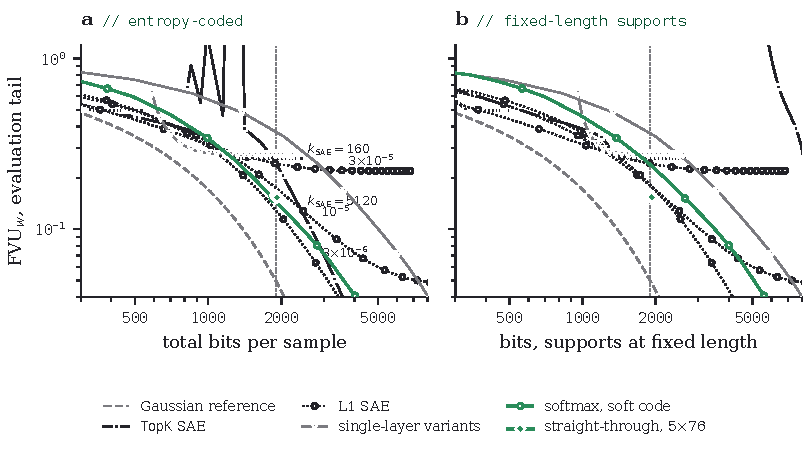
\includegraphics[width=\linewidth]{figures/fig-quantrate.pdf}
\caption{Operational rate on the evaluation tail: everything each code
sends quantized (Eq.~\eqref{eq:quantrate}) at a swept step, (a) each
slot's symbols entropy-coded and (b) each support charged its fixed-length
cost, the values still entropy-coded. L1 SAEs are labeled by
$s_{\mathrm{L1}}$; the unlabeled $\topk$ curve is
$k_{\mathrm{SAE}}{=}32$, and the single-layer variants are
\texttt{g160top1} (level) and \texttt{g160softmax} (falling). The
straight-through stack's curve spans 1895--1923 bits. The dotted line is
1900 bits and the dashed curve the Gaussian reference
(Eq.~\eqref{eq:ratefloor}). The softmax model saw the tail in training;
scored on rows no model saw, no curve's readout at 1900 bits moves by
more than 0.0004 (Appendix~\ref{app:data}). One seed per curve.}
\label{fig:quantrate}
\end{figure}

\subsection{Depth: eliminations and mechanism}
\label{sec:depthdetail}

\paragraph{Over training.} Scored held out at every 10k checkpoint
(Figure~\ref{fig:depth-curves}), the stack leads the flat arms from the
first checkpoint on: the ratio to the matched flat arm is $1.59\times$ at
step 10k, peaks at $1.83\times$ near 200k and ends at $1.79\times$.
Neither shape has converged. Over the last quarter the stack improves
$0.86\%$ and the flat arms $2.3$--$2.75\%$, so the gap is narrowing,
slowly; where it ends needs longer runs. Seed replicas overlap at every
checkpoint.

\begin{figure}[tp]\centering
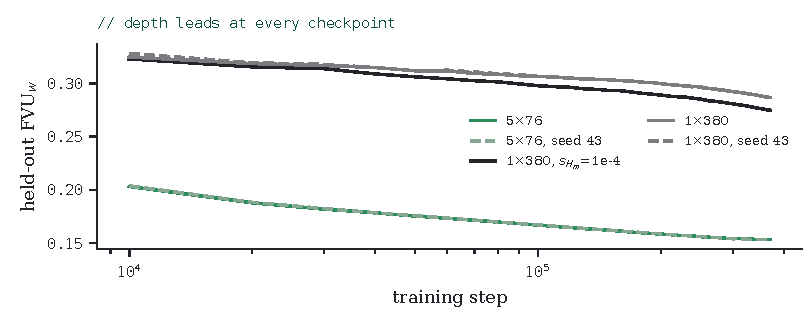
\includegraphics[width=\linewidth]{figures/fig-depth-curves.pdf}
\caption{Held-out $\fvu$ over training for the $5\times76$ stack and the
$1\times380$ flat arms at matched bits and parameters, with seed replicas.
The flat arm with the stack's entropy pressure ($s_{\mathrm{KL}_m}{=}10^{-4}$)
is the one compared in Section~\ref{sec:depth}.}
\label{fig:depth-curves}
\end{figure}

The comparison went through two wrong versions first, and the
eliminations are informative. On the shipped initialization the flat arm
read $0.5822$ at 484 realized bits (25.5\%), a $2.5\times$ gap. Correcting
the per-head entropy pressure --- $\mathrm{KL}_m$ averages over a layer's
heads and the loss sums over layers, so per-head pressure scales as
$s_{\mathrm{KL}_m}/h$ per layer and the flat arm had trained at a fifth of
the stack's --- took it to 1199 bits and $0.4307$. A frozen ZCA whitener
(\texttt{make\_zca.py}) took the classifier's input from effective
dimension 107 to 901 and the code to 1900 of 1900 bits, every head at
4.999 of 5 bits, more than the stack itself realized --- and still
reconstructed $1.7\times$ worse ($0.3842$). Two survivors from that line:
\textbf{usage is not what depth buys} (bits are not the objective either:
dropping $s_{\mathrm{KL}_m}$ 100$\times$ costs the stack 176 bits and
\emph{improves} its error to $0.2095$), and \textbf{a learned input
transform collapses where a supplied one does not} --- a jointly trained
\texttt{Linear} encoder ends with every head on exactly two entries at
$\fvu$ $0.6853$, worse than no encoder.

\paragraph{The input each classifier sees.} \texttt{inputgeom.py}, on the
exact vector handed to each classifier (shipped arm):

\begin{center}\small
\begin{tabular}{@{}lrrr@{}}
\toprule
layer & mean direction & mean pairwise cos & effective dim / 1024 \\
\midrule
0 & 0.5638 & 0.3146 & 107.5 \\
1 & 0.0932 & 0.0087 & 611.3 \\
2 & 0.1522 & 0.0233 & 596.3 \\
3 & 0.1983 & 0.0396 & 548.8 \\
4 & 0.2348 & 0.0553 & 507.1 \\
\bottomrule
\end{tabular}
\end{center}

Layer 0 (and every flat arm) classifies the raw cap; layers 1--4 classify
residuals that span over half the space. On the shipped arm, layer 0 was
the only layer whose heads left most entries unused (10.6 live entries, 216 bits,
against $\sim$375 for each later layer) --- a within-model control on
everything except the input.

\paragraph{What the cascade contributes: pairing.}
\texttt{blendablate.py} blends the subtracted term
$\mathrm{dec}(\mathbf{r}_\ell)$ in layer $\ell$'s input toward a reference with
the same marginals and none of the pairing --- another row's
reconstruction (shuffle), the mean, or Gaussian noise rescaled to the
shuffle's per-sample magnitude --- without retraining:

\begin{center}\small
\begin{tabular}{@{}lrrrrr@{}}
\toprule
blend & shuffle & mean & noise & eff.\ dim L1 (shuffle) & (noise) \\
\midrule
0.000 & 0.2292 & 0.2292 & 0.2292 & 499.1 & 499.1 \\
0.125 & 0.2460 & 0.2374 & 0.2426 & 476.0 & 504.7 \\
0.250 & 0.3084 & 0.2652 & 0.2838 & 394.2 & 518.3 \\
0.500 & 0.6910 & 0.4100 & 0.4665 & 193.4 & 539.6 \\
0.750 & 1.8154 & 0.7497 & 0.8502 & 103.0 & 527.6 \\
1.000 & 4.6613 & 1.4302 & 1.5992 & 68.5 & 496.2 \\
\bottomrule
\end{tabular}
\end{center}

The pairing is load-bearing well below full severance --- a quarter blend
costs 35\% of $\fvu$ --- and another row's reconstruction does more damage
than matched-magnitude noise at every level, so the damage is specific
rather than generic perturbation sensitivity. The sweep cannot separate
pairing from conditioning: effective dimension falls in lockstep with the
error, because a residual is small and nearly isotropic \emph{because} it
is this sample's own error. That resolves the whitened arm rather than
conflicting with it: whitening is conditioning without pairing, and it
bought uniform usage of every entry and $\sim$7\% of $\fvu$. (\texttt{forward="labels"},
which would test this by removing the residual entirely, has not been run
at the fixed initialization. Forwarding the code \emph{alongside} the
residual, \texttt{forward="resid\_labels"}, was a clear negative in a
three-epoch pilot: held-out $\fvu$ $0.826$ against $0.249$, after leading
early by $50\times$ --- the signature of a parameter advantage without an
information advantage, since the residual is by construction what the
code failed to explain.)

\paragraph{The code is not the whole channel.} Each layer splits its input
into a unit direction (all the classifier sees) and a norm that multiplies
the layer's output, so one real number per layer per sample reaches the
decoder outside the bottleneck. Pinning each gain to its held-out mean
(\texttt{gainablate.py}) costs the stack $+3.0\%$ in total, $+0.6$ to
$+0.8\%$ per layer (layer 0's gain is identically 1, since the cache is
L2-normalized; SONAR's own embeddings are not~\cite{sonar}), against the
79\% by which the matched flat arm trails it: the channel is real and is
not the explanation. With the gains pinned the stack is a pure 1900-bit
code ($\fvu$ $0.158$), the form compared against SAEs at matched total
rate in Section~\ref{sec:ste}. It does matter as a confound
for the whitened flat arm, whose whitener creates a varying layer-0 gain
worth $+4.5\%$ --- about 40\% of whitening's apparent benefit.

\paragraph{The decoder is dense, and not because of the offset.}
Magnitude-pruning the trained decoder's smallest half takes $\fvu$ into
the thousands, and its weight distribution looks like a Gaussian
matrix's. The non-negative dictionary makes the accumulator's constant
part dwarf its varying one ($\lVert\mathbb{E}\mathbf{r}\rVert /
\mathbb{E}\lVert \mathbf{r}-\mathbb{E}\mathbf{r}\rVert = 11.6$), and the
bias-free decoder does attenuate that constant
to the embedding mean (norm 0.581 against 0.564). But a decoder bias
(\texttt{--biased-dec}) is worth only $-0.62\%$ of training MSE at matched
step (the run died at 23\% of its schedule, so its held-out $0.2464$ is
not comparable to the converged arm's): pinning
$W_{\mathrm{dec}}\,\mathbb{E}\mathbf{r}$ is 1024 linear constraints on a $1024\times2048$ matrix,
0.05\% of its freedom. The decoder is dense because a full-rank map
carrying a $\sim$900-dimensional signal is dense.

\paragraph{How the layers' partitions relate.} Each head's winning entry
partitions the eval tail, and Figure~\ref{fig:headnmi} compares every
pair of the 380 heads of \texttt{ste\_h76} (shipped init;
\texttt{headnmi.py}). Heads partition independently except within layer
0: the mean adjusted NMI within a layer is 0.0075 at layer 0 and
0.0006--0.0028 above it, and at most 0.0004 between layers (GPT-2's
stack: 0.054 at layer 0, at most 0.004 elsewhere), so a later layer does
not re-split what an earlier one split. Effective information, how far
forcing one head moves another's choice, tracks that overlap only from
layer 0: over head pairs its Spearman correlation with adjusted NMI is
0.76, 0.50, 0.38 and 0.23 from layer 0 to layers 1--4, and at most 0.08
from any later layer, whose heads move every downstream head by a similar
0.003--0.02 bits whatever their partitions share. One seed.

\begin{figure}[tp]
\centering
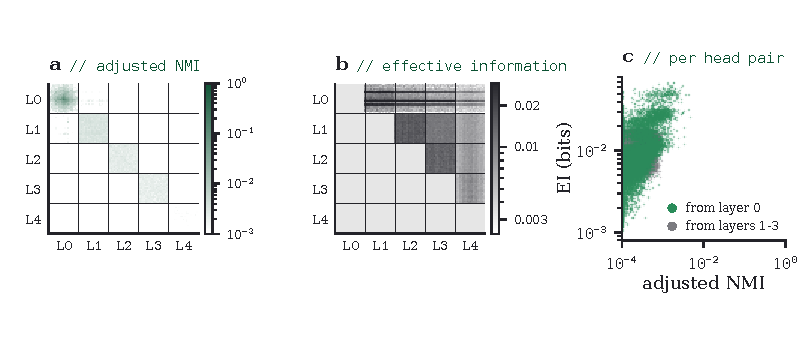
\includegraphics[width=\linewidth]{figures/fig-headnmi.pdf}
\caption[Head partitions against each other and against
intervention]{\textbf{Partitions overlap, and track intervention, only
	in layer 0.} \texttt{ste\_h76} (shipped init) on the eval tail, its 380
	heads blocked by layer and ordered within a layer by hierarchical
	clustering. (a) Adjusted NMI between every pair of heads'
	winning-entry partitions (0 = chance), log scale, diagonal grey.
	(b) Effective information from the row head to the column head, with
	interventions uniform over the source's live entries; grey where the
	effect head is not downstream. (c) One against the other per head
	pair, by source layer. One seed.}
\label{fig:headnmi}
\end{figure}

\subsection{Steering by target layer, and head-health levers}
\label{sec:steerlayer}

Splitting the stack's steering by target layer (strength 1.0, 12 entries
per layer) reverses the aggregate ranking of directions:

\begin{center}\small
\begin{tabular}{@{}lrrrrr@{}}
\toprule
layer & decode & grad & margin & adjoint & random \\
\midrule
0 & 0.216 & \textbf{0.583} & 0.547 & 0.237 & 0.034 \\
1 & 0.464 & 0.089 & 0.367 & 0.000 & 0.023 \\
2 & 0.742 & 0.130 & 0.216 & 0.000 & 0.055 \\
3 & \textbf{0.966} & 0.130 & 0.091 & 0.000 & 0.034 \\
4 & 0.362 & 0.047 & 0.036 & 0.005 & 0.047 \\
\bottomrule
\end{tabular}
\end{center}

Where the input reaches the classifier directly (layer 0), the
classifier's own geometry (\texttt{grad}, \texttt{margin}) beats
\texttt{decode} three- to tenfold. With depth it fails: a direction
computed against layer $\ell$'s classifier input is only valid there, and
the perturbation arrives after earlier layers have re-encoded it. The
\texttt{decode} direction moves the input toward what the model itself
emits with the entry active, which is self-consistent down the stack. Layer
4 is hard for everything: its residual is nearly exhausted. The practical
reading is to steer layer 0 by gradient and the middle layers by decode.

\paragraph{Head-health levers and steering.} Three levers were tried on
the shipped stack. \emph{Mean-entropy pressure is not what costs
steerability}: a twin trained at $s_{\mathrm{KL}_m}{=}10^{-6}$ has raw
text-cycle effect $0.043$ against $0.027$, both an order of magnitude
below \texttt{top2}/\texttt{top8} at the same weight, so hard selection,
not the bonus, is the cost (removing the bonus does cost head usage:
imbalance 5.00 bits against 2.71). \emph{Head-independence pressure
(HSIC/CKA) was chasing estimator bias} (Section~\ref{sec:hsic}).
\emph{A row-collinearity setpoint is the one lever that bought
steerability}: holding within-head row cosine at 0.5 (against an
uncontrolled 0.774) improves embedding-space realization in every
direction at lower collateral --- \texttt{decode} $+15\%$,
\texttt{grad} $+17\%$, \texttt{margin} $+52\%$, oriented
\texttt{adjoint} $+122\%$, collateral 0.591 $\to$ 0.552 --- with held-out
$\fvu$ slightly better ($0.2157$ vs.\ $0.2293$). The controller acts once
(Figure~\ref{fig:kcos}): as the max row cosine over heads and layers
climbs past 0.8, the multiplier rises to $4.9\times10^{-3}$ near step 35k
and pulls it down to the setpoint by 50k; from about 60k the multiplier
is projected to zero and the statistic stays at or below 0.5 without
pressure, ending at 0.473 against the uncontrolled 0.774. Its mechanism
is unexplained: the
statistic is computed in the $e$-dimensional dictionary space, where
74--78\% of each atom's energy is in the decoder's null space
(Section~\ref{sec:rowcos}), and decoded the atoms were already
orthogonal. That the classifier-geometry directions gain most suggests
an effect on the classifier rather than the dictionary, but nothing
establishes it. The setpoint does not transport to the flat arm, whose
steering is already saturated (0.992 vs.\ 0.966).

\begin{figure}[tp]\centering
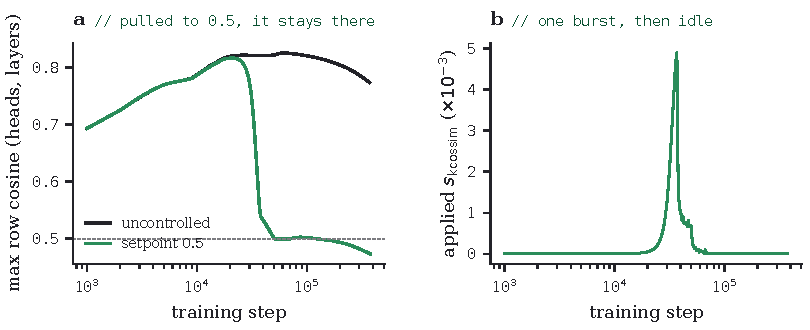
\includegraphics[width=\linewidth]{figures/fig-kcos.pdf}
\caption{The row-collinearity setpoint on the shipped stack, from the
training log. (a) The max within-head row cosine over heads and layers,
the statistic the controller watches, against the uncontrolled twin; the
dotted line is the 0.5 setpoint. (b) The applied multiplier
$s_{\mathrm{kcossim}}$, averaged over 1000-step windows.}
\label{fig:kcos}
\end{figure}

\subsection{Supervised vectors at their own step size}
\label{sec:steersupnative}

Table~\ref{tab:steersup} compares directions at an equal step. A real
intervention has its own length: for a model, the output change of
forcing the entry; for an SAE latent, its decoder direction at its mean
activation; for the difference of means, the difference vector itself,
which is the step activation addition takes. At those lengths (realized /
collateral, median step as a fraction of $\lVert\mathbf{x}\rVert$, and each
equal-length random step's collateral):

\begin{center}\small\setlength{\tabcolsep}{4pt}
\begin{tabular}{@{}lrrr@{}}
\toprule
model & \stackhead[r]{own\\(step)} & \stackhead[r]{diff.\ of means\\(step)}
& \stackhead[r]{random:\\own / dm} \\
\midrule
softmax stack & 0.19 / 0.25 (0.064) & 0.18 / 0.25 (0.079) & 0.25 / 0.30 \\
hard-code stack & 0.08 / 0.54 (0.129) & \textbf{0.27} / 0.47 (0.064) & 0.53 / 0.48 \\
hard-code flat & 0.17 / 0.04 (0.028) & \textbf{0.54} / 0.12 (0.087) & 0.05 / 0.17 \\
\texttt{g160top1} & 0.41 / \textbf{0.01} (0.186) & 0.57 / 0.04 (0.053) & 0.18 / 0.07 \\
\texttt{g160softmax} & 0.54 / 0.07 (0.050) & 0.57 / 0.13 (0.107) & 0.08 / 0.16 \\
$\topk$ SAE, $k_{\mathrm{SAE}}{=}32$ ($m{=}5120$) & 0.46 / 0.06 (0.072) & \textbf{0.77} / 0.15 (0.180) & 0.07 / 0.17 \\
$\topk$ SAE, $k_{\mathrm{SAE}}{=}32$ ($m{=}11264$) & 0.50 / 0.08 (0.076) & \textbf{0.82} / 0.17 (0.172) & 0.09 / 0.19 \\
SAE, bilinear encoder & 0.82 / 0.04 (0.078) & 0.88 / 0.08 (0.121) & 0.04 / 0.07 \\
\bottomrule
\end{tabular}
\end{center}

The difference of means realizes more in most models, and in the SAEs and
the flat arm partly by taking 2--3 times longer steps. The hard-code stack
is the clear case where direction, not length, decides: the supervised
vector reaches its entries three times as often with half the step. The
softmax stack's own intervention and the supervised vector tie.
\texttt{g160top1}'s own intervention is the most precise step any method
takes, disturbing 1.4\% of other heads against 18\% for random.

\subsection{Data-shaped controls, and where a decode step realizes}
\label{sec:steernull}

Every steering curve is scored against an isotropic random step. SONAR's
evaluation tail is anisotropic --- 158 of its 1024 principal components
hold half its variance, 474 hold 80\% --- so a unit step in raw
coordinates is three times as long in the data's own (Mahalanobis) metric
as a step shaped like the data, each relative to the distance between two
tail rows, while the objective's diagonal whitening barely registers the
difference (1.045 against 1.005). \texttt{steerembed.py} also scores three
random controls of the same raw length: the isotropic draw shaped by the
covariance's square root, the same draw shaped by its inverse square root
(toward what the data barely vary along), and the step toward another
tail row. Collateral at strength 0.25, on the targets and rows of
Table~\ref{tab:steersup}:

\begin{center}\small\setlength{\tabcolsep}{4pt}
\begin{tabular}{@{}lrrrrrr@{}}
\toprule
model & isotropic & shaped & to a row & inverse & decode & diff.\ of means \\
\midrule
softmax stack   & 0.539 & 0.408 & 0.410 & 0.803 & 0.549 & 0.424 \\
hard-code stack & 0.653 & 0.634 & 0.640 & 0.754 & 0.658 & 0.629 \\
hard-code flat  & 0.367 & 0.315 & 0.309 & 0.521 & 0.328 & 0.274 \\
\bottomrule
\end{tabular}
\end{center}

Against the data-shaped steps the softmax stack's decode direction
disturbs 0.14 more heads, and its gradient, margin and adjoint directions
0.15--0.20 more, though all are within 0.07 of the isotropic step. In the
hard-code stack every direction stays within 0.025 of the data-shaped
steps. In the flat arm the decode direction and the difference of means
stay within 0.041 of them, and the gradient-based directions sit 0.06--0.07
above, at the isotropic level. Steps toward what the data barely vary
along disturb the most heads in every model.

Splitting the decode direction at the leading principal subspace holding
50\% or 80\% of the variance, and stepping each part at the full step's
length, locates what realizes the target. In both stacks the part in the
bottom fifth of the variance realizes 95\% (hard) and 100\% (softmax) of
what the full step does, and the part in the top half 20\% and 8\%; the
flat arm realizes through either part (0.958 from the top 80\% alone,
against 0.996). The decode direction leans toward the low-variance end:
the data's variance along it is 1.6--1.8 times the mean eigenvalue,
against 6.2--6.7 for a data-shaped step and 7.1--11.7 for the difference
of means. That is the sensitivity to directions the data barely vary
along which Ilyas et al.~\cite{ilyas2019} tie to non-robust features.
Equal raw length is the budget used throughout, so the split says where
the classifiers are sensitive per unit of raw length; whether the SONAR
decoder reads the low-variance part is untested. One seed per model.

\subsection{What a removal does downstream}
\label{sec:removals}

Removing a head shows what the cascade does with a change it did not
choose (\texttt{textstrip.py --removals}). For 16 random heads per layer
on 512 tail rows, each head's assignment is replaced by the uniform one,
by the head's mean assignment, by its runner-up entry (what winner
dropout trains on) or by another row's assignment, and the
reconstruction is rebuilt either live, with later layers reclassifying
the changed residual, or frozen, with only that head's contribution
changed. Two readouts, whitened and each a share of the unablated
reconstruction's error: the error the removal adds, and how far the
output moves from the unablated reconstruction. In the hard-code stack
the live forward cuts a layer-0 head's added error to 0.23 of the frozen
value (0.48, 0.68 and 0.84 at layers 1--3), and cuts the runner-up
replacement most (0.13), as backup heads take over a knocked-out head's
role in IOI~\cite{wang2023ioi}. Yet the live output lands 19 times as far
from the unablated reconstruction as the frozen one (31, 19 and 7 times
at layers 1--3): the later layers describe the input anew rather than
restore the old description. Decoded to text, on 12 tail rows and the
two heads per layer whose uniform removal moves the reconstruction
furthest, a live uniform removal raises the decoder's per-token negative
log-likelihood of the input's own decoding by nothing beyond the
reconstruction's ($-0.011$ nats, against 0.036 frozen and 0.016 for a
random step toward another row of the frozen change's length), though
scored against the unablated reconstruction's text it looks like damage
(0.139 against 0.040). The reference softmax model's later layers cancel
a removal outright: a frozen layer-0 uniform removal adds 505\% to the
error and a live one 0.5\%. These text runs compute the model in float32
on the CPU; JAX's default matmul precision on the GPU changes 226 of the
hard stack's 4{,}560 codes on these 12 rows (159 of the 912 at layer 4),
so cell-level comparisons across devices need matched precision. One
seed per model.

\subsection{Head independence: a measurement artifact}
\label{sec:hsic}

A head-independence penalty (\texttt{--s-hsic-heads}: the mean over a
layer's head pairs of RBF-kernel CKA~\cite{kornblith2019} between the
heads' batch assignments, at the median-heuristic bandwidth) appeared to
find substantial dependence. It was measuring bias: CKA as defined there
normalizes the biased HSIC estimator~\cite[Eq.~3]{kornblith2019}, which
is positive for independent heads:

\begin{center}\small
\begin{tabular}{@{}lrrrrrr@{}}
\toprule
layer & 0 & 1 & 2 & 3 & 4 & mean \\
\midrule
unbiased & 0.0041 & 0.0005 & 0.0005 & 0.0004 & 0.0002 & \textbf{0.0011} \\
biased   & 0.0315 & 0.1062 & 0.1018 & 0.0963 & 0.0976 & 0.0867 \\
\bottomrule
\end{tabular}
\end{center}

The biased estimator reads chance co-occurrence between independent
categorical heads as dependence, with a floor that grows as the batch
shrinks (0.109 at $b{=}256$, 0.029 at 1024, against an unbiased 0.0001 at
every size). The floor also falls with the number of entries a head
uses, and a frozen head, whose constant code depends on nothing, scores
zero against every other: on synthetic independent heads at $b{=}256$
and $k{=}32$ it reads 0.108 at uniform usage, 0.016 at about four
effective entries, and 0.026 with half the heads frozen
(\texttt{cka\_floor.py}). At the training batch the floor exceeded any
real dependence, so the penalty had nothing to descend but the bias, and
the bias descends only by concentrating or freezing heads.
Reconstruction resisted that here; where the penalty replaced the
softmax model's auxiliary losses, it froze a layer
(Section~\ref{sec:freeze}).
\texttt{hsic.pairwise\_head\_cka} now normalizes Song et al.'s unbiased
estimator~\cite[Eq.~5]{song2012} instead (``debiased'' CKA, as in the
minibatch CKA of~\cite{nguyen2021}); its expectation is exactly zero for
independent heads at any batch size, and it reads 0.06 at 0.5 planted
factor correlation and 0.41 at 0.8. Conditioning on language or script explains
none of the residue. \textbf{This architecture produces near-independent
heads with no pressure to do so}; trained out under the corrected
estimator the penalty changes nothing and costs localization
(best-head language NMI 0.199 against 0.269). Two lessons generalize:
before trusting a statistic as a training signal, measure it on a null
it should score zero on; and loss-value share is not gradient share ---
at $s_{\mathrm{HSIC}}{=}10^{-4}$ the penalty was 12\% of the loss value, while the
measured MSE-to-CKA gradient ratio (1250 at the classifier, 221 at the
dictionary) put equal pull at $8\times10^{-4}$.

\subsection{Seed reproducibility, measure by measure}
\label{sec:seedsdetail}

\emph{Partitions.} The best-matched pair of heads reaches NMI 0.42, but
the mean is 0.012 against a 0.005 null, and \texttt{splitting.py}'s entry
containment reads 0.000. Neither is a metric artifact: comparing one run
against its own checkpoint 19{,}500 steps earlier, the same partition
measure scores 0.38 overall and 0.87 on layer 0. \emph{Contributions.}
Two heads could carve differently and add the same thing; they do not
(centered cosine 0.0074 vs.\ 0.0015 null; uncentered it reads 0.205, which
is the non-negative dictionary's shared offset). \texttt{headcontrib.py},
which fixes the measurement (decoded, whitened, centered contributions,
Hungarian-matched), reads $0.019$ against a $0.0017$ null on the same
pair at 4{,}096 rows; the earlier one-off figure's exact method was not
recorded, and the conclusion is unchanged under either. \emph{Subspaces.}
Top-8 eigenspaces of per-layer contributions agree 25--33$\times$ above
chance --- but each model agrees with the \emph{cache's own} principal
directions by the same amount (e.g.\ layer 1: 123.7$\times$ between
seeds, 101.3$\times$ and 101.2$\times$ to the data), so the agreement is
the data's and nothing is left for the architecture. At layer 4 each
seed tracks the data $\sim$23$\times$ above chance while agreeing with the
other only 9$\times$: they pick \emph{different} data-aligned directions.
\emph{Grams} (\texttt{atomgram.py}). Per-layer row collinearity agrees
to four digits (0.2880 / 0.2891 at layer 0), but the Gram spectrum is
nearly one-parameter --- the top eigenvalue is exactly
$1+(k-1)\,\kappa_i$, carries 82\% of the spectrum's norm, and is forced
by non-negativity. Comparing two heads' Grams entrywise needs a
correspondence between their entries. In canonical order (each head's
entries sorted by their mean cosine to the rest of the head), Grams agree
at chance against a null that pairs heads within the layer, across seeds
(1.06--1.11$\times$) and against the same run 19{,}500 steps earlier
alike (1.05--1.14$\times$). The second is a property of the order, not of
the heads: with a nearly one-parameter Gram every entry's mean cosine is
nearly the same, so the sort is set by small differences that change
between checkpoints, and within one run it pairs only 33--66\% of heads
with themselves. Training never relabels entries (dead-entry revival is
off in both runs), so within a run the stored order is the
correspondence, and in it each head's Gram matches its earlier self at
8.5--10.7$\times$ chance (7.5--10.0$\times$ on decoded atoms), its
decoded atoms at cosine 0.98--0.99 against 0.05--0.08 for the layer's
other heads. Across seeds, with entries matched by linear assignment on
their centered decoded atoms, which fixes the correspondence exactly,
Grams stay at chance (1.05--1.19$\times$), the matched atoms at cosine
0.07--0.15 against 0.06--0.10. Heads persist within a run and do not
replicate across seeds.

\subsection{What makes layer 0 reproduce: gain, atoms, and depth}
\label{sec:l0size}

Layer-0 heads are the largest and the most reproducible, so ``layer 0
reproduces'' might be ``large heads reproduce''. \texttt{headcontrib.py}
measures a head's size as its centered contribution energy over the
whitened target variance, and splits it exactly: a head's contribution on
a row is its layer's input gain times the decoded atom it selected, so
its size is gain$^2$ times atom spread$^2$ (the usage-weighted RMS
distance of its decoded atoms from their mean); on both stacks the
product reproduces the measured size to a log correlation of 1.000.

\begin{table}[htbp]\centering\small
\begin{tabular}{@{}lrrrrrr@{}}
\toprule
& \multicolumn{3}{c}{GPT-2 concat} & \multicolumn{3}{c}{SONAR stack} \\
layer & agreement & gain & atom norm ($10^{-4}$) & agreement & gain & atom norm \\
\midrule
0 & 0.171 & 122.2 & 4.6 & 0.080 & 1.000 & 0.043 \\
1 & 0.017 & 67.9 & 5.3 & 0.005 & 0.588 & 0.054 \\
2 & 0.007 & 62.3 & 4.4 & 0.004 & 0.490 & 0.052 \\
3 & 0.005 & 59.2 & 3.7 & 0.003 & 0.417 & 0.051 \\
4 & 0.004 & 57.2 & 3.2 & 0.003 & 0.359 & 0.043 \\
\bottomrule
\end{tabular}
\caption{Head agreement (matched centered contribution cosine) and the
two factors of head size, medians over each layer's heads; atoms decoded
and whitened. SONAR: \texttt{ste\_h76\_init01} against
\texttt{ste\_h76\_i01\_s43}, 4{,}096 rows.}
\label{tab:gainatoms}
\end{table}

\textbf{Layer 0's larger contributions are all gain.} It receives the raw
input --- GPT-2 activations of norm $\sim$122 against residuals of
$\sim$60; unit SONAR embeddings against residuals of 0.36--0.59 --- while
its atoms are no larger than layer 1's on either dataset, and on SONAR
smaller than those of layers 1--3 and equal to layer 4's. Gain is one
number per layer per row, shared by all of a layer's heads, so across
layers ``size'' is the layer itself under another name. At equal atom
spread, layer 0 still reproduces $14\times$ better on GPT-2 and $23\times$
better on SONAR (log agreement on log spread and a layer-0 indicator,
coefficient of determination 0.979 and 0.941).

\paragraph{Against the flat arm at matched size.} Within a stack, head
size and layer do not overlap, so their effects cannot be separated
there. The flat arm breaks the confound: all its heads see the raw input,
with gain 1 and nothing downstream. On SONAR its own agreement tracks
log head size at correlation $0.876$ --- from $0.008$ for its smallest heads
(0.057--0.060\% of target variance) to $0.150$ above 0.071\%, and $0.78$
and $0.56$ for its two largest --- so size matters a great deal on its
own, and since its gain is constant it is an atom-magnitude curve. But
the stack's heads fall far below that curve at every depth, layer 0
included:

\begin{center}\small
\begin{tabular}{@{}lrrrr@{}}
\toprule
stack layer & size, median & stack agreement & flat heads at that size ($\pm$10\%) & gap \\
\midrule
0 & 0.31\% & 0.080 & 0.67 (2 heads) & $\sim$8$\times$ \\
1 & 0.16\% & 0.005 & 0.12 (1 head) & $\sim$23$\times$ \\
2 & 0.11\% & 0.004 & 0.19 (3 heads) & $\sim$49$\times$ \\
3 & 0.073\% & 0.003 & \textbf{0.059} (115 heads) & $\sim$\textbf{19}$\times$ \\
4 & 0.039\% & 0.003 & below the flat range & --- \\
\bottomrule
\end{tabular}
\end{center}

\textbf{The stack costs reproducibility at matched size, at every
layer.} Layer 0 sees exactly the flat arm's input and still reproduces
several times worse than an equal-size flat head: in the stack, what a
layer-0 head should carve depends on what the layers after it do with
its error, so the input alone no longer pins it. Deeper layers lose
more. This is the reproducibility face of the entanglement result
(Section~\ref{sec:entangle}): the cascade that doubles a single-head
intervention's collateral, to 66\% of the other heads, also leaves each
head underdetermined by the data. Read against the flat curve, the gain
difference between layers 0 and 3 accounts for roughly a third of layer
0's lead in log terms; only layer 3's size match is solid --- flat heads
are almost all small, so layers 0--2 rest on one to three heads each ---
so the fraction is rough and the direction firm. The matched-size
comparison is SONAR-only; GPT-2 has no flat arm.

\paragraph{Within layer 0 the atoms decide.} SONAR's layer-0 gain is
identically 1, so its within-layer size variation is pure atom
magnitude, and there log agreement tracks atom norm at correlation $0.62$
and spread at $0.64$ (cosine against log size, $0.91$); GPT-2's layer 0 shows
$0.17$ and $0.42$. Past layer 1 the atoms predict nothing on either
dataset. Spread and norm are one quantity here --- their ratio is
0.99--1.08 in every layer, so a head's usage-weighted mean decoded atom
is near zero: the non-negative dictionary's offset is cancelled by the
decoder before it reaches the output.

\subsection{How entries share a layer}
\label{sec:entries}

An entry writes only where it wins its head, and then writes its layer's
gain times its decoded atom, so its energy over the data is
$\mathbb{E}\big[\mathbf{1}[\text{selected}]\,\mathrm{gain}^2\big]\,
\lVert\text{atom}\rVert^2$. Per layer, over 32{,}768 held-out rows
(\texttt{entryshare.py}):

\begin{table}[htbp]\centering\small
\begin{tabular}{@{}llrrrrr@{}}
\toprule
run & layer & Gini & \stackhead[r]{top 10\%\\carry} & \stackhead[r]{max/\\median}
& \stackhead[r]{from atom\\norm} & \stackhead[r]{within\\heads} \\
\midrule
GPT-2 concat, $k{=}256$ & 0 & \textbf{0.587} & 42\% & 38.7 & 76\% & 60\% \\
& 1 & 0.155 & 16\% & 30.3 & 44\% & 100\% \\
& 2--4 & 0.11--0.12 & 14\% & $\sim$2 & $\sim$40\% & 100\% \\
SONAR stack, $k{=}32$ & 0 & \textbf{0.326} & 32\% & 46.3 & 92\% & 83\% \\
& 1--3 & 0.06--0.10 & 12--14\% & 1.5--1.9 & 16--24\% & $\sim$100\% \\
& 4 & 0.195 & 18\% & 3.2 & 77\% & 87\% \\
SONAR flat, $1\times380$ & --- & 0.190 & 23\% & 64.1 & 90\% & 76\% \\
\bottomrule
\end{tabular}
\caption{Inequality of entry energy within a layer. ``From atom norm'' is
the covariance share of the variance of log entry energy (the remainder
is usage; gain conditional on selection contributes $\sim$0). ``Within
heads'' is the share of that variance not explained by which head an
entry is in. No entry is dead in any layer.}
\label{tab:entries}
\end{table}

\textbf{Layers 1--3 are near-equal; layer 0 is not, and its atoms are
why.} Deep entries have an effective number of 95--99.5\% of the total
and the largest is about twice the median; what inequality they have is
mostly usage, itself mild (CV 0.14--0.18). Layer 0's usage is just as
even --- on SONAR every entry fires 2.1--4.5\% of the time against $1/k =
3.1\%$ --- but its atom norms vary five to ten times more (CV 0.34--0.52
against 0.02--0.10), mostly inside heads. The flat arm shows the same
pattern more mildly, so it belongs to classifying the raw input. SONAR's
last layer is unequal for the other reason: some atoms have shrunk almost
to nothing (smallest/median 0.017), the inert final layer of
Section~\ref{sec:lastlayer}. Whole layers are unequal by gain: layer 0
holds 67\% of entry energy on GPT-2 and 49\% on SONAR, layer 4 4--5\%.

\paragraph{Where the large atoms sit} differs completely between the
models (\texttt{bigatoms.py}):

\begin{center}\small
\begin{tabular}{@{}>{\raggedright\arraybackslash}p{0.34\linewidth}%
>{\raggedright\arraybackslash}p{0.28\linewidth}%
>{\raggedright\arraybackslash}p{0.28\linewidth}@{}}
\toprule
& GPT-2 concat, 20 heads & SONAR stack, 76 heads \\
\midrule
\multicolumn{3}{@{}l}{\emph{within a head} (atom norm $/$ the head's own median, mean over heads)} \\
\quad largest & 3.7 (1.4--5.1 across heads) & 2.0 (1.5--4.3 across heads) \\
\quad 2nd / 8th / 16th largest & 3.2 / 2.0 / 1.7 & 1.7 / 1.2 / 1.0 \\
\quad largest entry's share of head energy & 6.1\% (uniform 0.4\%) & 9.9\% (uniform 3.1\%) \\
\multicolumn{3}{@{}l}{\emph{across the layer} (atom norm $/$ the layer median)} \\
\quad atoms $>2\times$ & 1030 (20\%), in all 20 heads & 63 (2.6\%), in 28 heads \\
\quad atoms $>3\times$ & 58, in \textbf{all 20} heads (at most 15 each) & 11, in \textbf{4} heads \\
\quad atoms $>5\times$ & 1 & 5, \textbf{all in head 54} \\
\quad largest head's energy share & 15.5\% (3$\times$ uniform) & 9.2\% (7$\times$ uniform) \\
\multicolumn{3}{@{}l}{\emph{usage}} \\
\quad Spearman(atom norm, usage) in heads & $+0.81$ & $+0.27$ ($-0.04$ to $+0.58$) \\
\quad usage of atoms $>3\times$ / of the rest & 0.0062 / 0.0037 ($1/k$ 0.0039) & 0.033 / 0.031 ($1/k$ 0.031) \\
\multicolumn{3}{@{}l}{\emph{direction}} \\
\quad $|\cos\angle|$ between heads' largest atoms & 0.022 (random pairs 0.048) & 0.023 (random pairs 0.028) \\
\quad energy in the data's top 10 PCs & 4\% (all atoms 13\%) & 9\% (all atoms 3\%) \\
\bottomrule
\end{tabular}
\end{center}

On GPT-2 every head has a graded tail --- its eighth-largest atom is
still twice its median --- and the large atoms are its frequent outcomes
(1.6$\times$ uniform usage). Agreement is fairly even across heads
(0.135--0.235) and only loosely tied to atoms (Spearman 0.49 with energy
share, 0.34 with the largest atom). On SONAR the large atoms are a few
heads' property, and fire at the uniform rate: large, not frequent. Head
54 holds 8 of the 11 atoms above $3\times$ and all 5 above $5\times$,
carries 9\% of the layer, and reproduces at \textbf{0.844} against 0.249
for the next head; across heads, agreement tracks the largest atom
(Spearman 0.62) and how peaked the head's profile is (0.62), not its
typical atom ($-0.14$). That resolves the within-layer-0 atom effect into
a few heads with outsized atoms --- but not the layer-0 lift: without head
54 the layer-0 mean falls only from 0.080 to 0.070, still twenty times
the deep layers. Head 54 is the topic/genre head of
Section~\ref{sec:lang}, which recurs across seeds.

\begin{table}[htbp]\centering\small
\begin{tabular}{@{}lrrrrr@{}}
\toprule
head & agreement & \stackhead[r]{energy\\share} & \stackhead[r]{largest $/$\\layer median}
& \stackhead[r]{atoms\\$>3\times$} & \stackhead[r]{largest $/$\\head median} \\
\midrule
\multicolumn{6}{@{}l}{\emph{SONAR stack, layer 0} (uniform share 1.3\%)} \\
54 & \textbf{0.844} & 9.2\% & 6.81 & 8 & 3.41 \\
46 & 0.249 & 2.5\% & 3.21 & 1 & 2.24 \\
6  & 0.181 & 1.5\% & 2.76 & 0 & 2.83 \\
18 & 0.150 & 1.9\% & 4.50 & 1 & 4.34 \\
\quad lowest four & 0.008--0.021 & 1.0--1.1\% & 1.51--1.84 & 0 & 1.48--1.84 \\
\midrule
\multicolumn{6}{@{}l}{\emph{GPT-2 concat, layer 0} (uniform share 5\%)} \\
6  & 0.235 & 3.1\% & 4.31 & 2 & 4.77 \\
17 & 0.220 & 15.5\% & 4.99 & 5 & 1.90 \\
19 & 0.215 & 3.4\% & 3.82 & 3 & 4.16 \\
0  & 0.202 & 3.1\% & 3.95 & 1 & 4.19 \\
\quad lowest four & 0.135--0.141 & 2.6--3.0\% & 3.13--4.17 & 1--2 & 3.45--4.56 \\
\bottomrule
\end{tabular}
\caption{Layer-0 heads by seed agreement (\texttt{bigatoms.py}; matched
centered contribution cosine against the seed-43 twin). Spearman of
agreement across heads, SONAR / GPT-2: with energy share $+0.53$ /
$+0.49$; with the largest atom $+0.62$ / $+0.34$; with the head's peakedness
(largest $/$ head median) $+0.62$ / $+0.09$; with its median atom $-0.14$ /
$+0.16$.}
\label{tab:bigatoms}
\end{table}

The two models differ in kind here. On SONAR one head stands out on every
atom measure and alone reproduces strongly; the rest of layer 0 is a
long, nearly flat tail, and agreement follows how peaked a head's atoms
are. On GPT-2 no head stands out: every head has several large atoms, the
spread of agreement is narrow, and the head with the largest share of the
layer's energy (17) has a flat profile --- uniformly large atoms rather
than a few outsized ones --- yet reproduces no better than its
neighbors. Peakedness predicts nothing there ($+0.09$).

The large atoms are distinct directions: different heads' largest atoms
are near orthogonal (median $|\cos\angle|$ 0.022--0.023, below random atom
pairs). On SONAR they lean into the data's top ten principal directions
(9\% of their energy against 3\% for a typical atom), consistent with
cross-seed agreement being the data's dominant directions; on GPT-2 they
lean the other way (4\% against 13\%). One seed pair per dataset
throughout.

\subsection{Language: the probe in detail}
\label{sec:langdetail}

Held-out language identity over 86 languages (dense ridge ceiling 0.721,
chance 0.012):

\begin{table}[htbp]\centering\small
\begin{tabular}{@{}llrrrr@{}}
\toprule
arm & shape & best-head NMI & less null & probe $h'{=}1$ & $h'{=}32$ \\
\midrule
\texttt{ste\_h76\_init01} & $5\times76$ & 0.180 & 0.169 & 0.103 & 0.420 \\
\quad seed 43 & $5\times76$ & 0.165 & 0.154 & 0.089 & 0.430 \\
softmax reference & $5\times32$ & 0.055 & 0.044 & 0.036 & 0.275 \\
\midrule
\multicolumn{6}{@{}l}{\emph{unfixed initialization}} \\
\texttt{ste\_h76} & $5\times76$ & 0.269 & 0.261 & 0.165 & 0.385 \\
\quad + collinearity setpoint & $5\times76$ & 0.287 & 0.279 & 0.139 & 0.317 \\
\quad $-$ mean-entropy bonus & $5\times76$ & 0.085 & 0.078 & 0.038 & 0.321 \\
\quad + head independence & $5\times76$ & 0.199 & 0.189 & 0.097 & 0.389 \\
flat & $1\times380$ & 0.277 & 0.276 & 0.102 & 0.259 \\
\quad + collinearity setpoint & $1\times380$ & 0.247 & 0.246 & 0.080 & 0.273 \\
\bottomrule
\end{tabular}
\caption{\texttt{headlang.py}. Heads are ranked by NMI on the
probe-training rows and scored on the held-out tail, and each probe's
ridge penalty is chosen on a validation split of the training rows. The
attainable NMI for a 5-bit head against the 6.43-bit label is 0.875.
Head-health levers and the flat arm were measured only at the unfixed
initialization.}
\label{tab:headlang}
\end{table}

As expected of a language-agnostic embedding, no head encodes language
outright: the best reaches 0.18 of an attainable 0.875, and no head-health
lever lifts any arm past 0.29 (a $k{=}32$ head could not hold 86
languages anyway, $\log_2 32 = 5 < 6.43$ bits). What the probe does show
is that partitions carry a known factor well above chance, and that
\textbf{the hard code carries more of it}: 3.5--3.9 times the softmax
reference on null-corrected best-head NMI, and 0.42--0.43 against 0.27
in a 32-head probe, consistently across seeds. The fixed initialization
spreads language over more heads than the unfixed one did
(null-corrected best head 0.15--0.17 against 0.26, 32-head probe
0.42--0.43 against 0.38). The stack beats the flat arm on probe accuracy at every head
budget (0.385 vs.\ 0.259 at $h'{=}32$, both unfixed).

\emph{Completeness.} The top 32 heads, all in layer 0, read 0.42--0.43,
73--74\% of what all 380 read (0.57--0.58), but they are not complete in
the sense of IOI's circuit criterion~\cite{wang2023ioi}, under which
removing them should leave the rest of the code unable to do the task:
the other 348 heads still read 0.34--0.36, the other 44 layer-0 heads
alone 0.26, and the 304 deeper heads together 0.13 (32 random deeper
heads, 0.03). Language is spread over layer 0, not held by a few heads. (\texttt{summary.json}'s
\texttt{info\_share\_best} favors the flat arm, but it divides by summed
plug-in MI whose per-head bias differs eightfold between the shapes; do
not read it across architectures.)

\paragraph{Script, cells, conjunctions.} Script behaves the same way
(best-head NMI 0.191 of a 0.671 ceiling; the same head, L0 h50, is best
for both). A single cell is a strong but permissive detector: the best
cell per language reaches recall 0.74--0.98 at FPR 1.6--2.2\%, but no
language reaches precision 0.8. Conjunctions of top cells from distinct
heads do not fix it: F1 peaks at $h'{=}2$ conjoined cells, 7\% above a
single cell, and the best precision is 0.598 at 4.8\% recall. Recall
combines nearly independently (0.234 against 0.262 predicted) but false
positives do not (precision 0.43 at $h'{=}2$ against 0.83 if independent): many heads send
the same confusable rows to the same wrong language --- Finnish with
Estonian, Japanese with Korean. The code encodes language
\emph{neighborhood} rather than identity.

\paragraph{Why neighborhoods, from the embedding geometry.} The
language-agnostic training leaves exactly the residue this pattern
implies. Language explains 6.51\% of embedding variance and script
2.26\%; corrected for the number of classes (\texttt{headeta.py}) language is still a
stronger partition than 90\% of the heads (51$\times$ its random baseline,
against 5$\times$ for the median head and 235$\times$ for the best), but its
languages are weakly separated regions, not directions: within-language
mean cosine is 0.3596 against 0.3160 between, and the shared mean
direction accounts for 0.3178 of that, leaving a $+0.044$ excess, 0.30 sd
of the pair distribution. A partition code cuts along local residual
variance, and at 0.30 sd those cuts pass through the language clusters
rather than around them. Layer-4 heads are near-random
partitions (2$\times$ baseline), which is Section~\ref{sec:lastlayer}'s
inert final layer seen from a different direction.

\paragraph{The topic head's entries.} Decoding and autointerp
were run on the shipped-initialization run's head 54, the head that holds
the same index in the fixed-initialization run (Section~\ref{sec:lang}).
Decoded as deviations from the head's mean atom, its entries read as
topic and genre. Contrastive autointerp (null 0.273) groups them
as genre or topic (16 entries, F1 0.523), multilingual or code-switched
passages (8, 0.476), text artifacts such as duplication and mojibake (3,
0.395), and script or region (5, 0.394); all four beat the null.

\section{Supplementary results: GPT-2 hard codes}
\label{app:gpt2}

\subsection{What each design change buys}
\label{sec:gpt2ablation}

One-epoch runs (10M tokens) isolate them:

\begin{center}\small
\begin{tabular}{@{}lrr@{}}
\toprule
variant (800 bits unless noted) & $\fvu$ & loss recovered \\
\midrule
STE alone (latent dictionary + decoder) & 0.327 & 93.3\% \\
+ gain & 0.290 & 94.3\% \\
+ gain, private heads & 0.288 & 94.2\% \\
+ gain, direct atoms & \textbf{0.217} & \textbf{96.95\%} \\
\quad seed 43 & 0.219 & 96.85\% \\
\quad $k{=}64$ (960 bits) & 0.186 & 97.6\% \\
\quad $k{=}128$ (1120 bits) & 0.165 & 97.9\% \\
\bottomrule
\end{tabular}
\end{center}

Gain-shape and direct atoms each help, and direct atoms most. Their
advantage is partly speed: over 40M tokens private heads close the gap and
finish slightly ahead (0.186 against 0.195). Without direct atoms and
gain, more entries per head collapse rather than help ($\fvu$ 0.75 and 0.80
at $k{=}64$ and 128), and the other straight-through configurations froze
their last layer at 4.8--5.0 bits, every head constant; the direct code's
deepest layer never froze. The base result reproduces across seeds to
0.002 $\fvu$. Annealing matters: straight-through at a constant $t{=}1$
reaches 0.50 and a scheduled soft-to-hard mix 0.39. Sparse encoders in
front of the classifier never beat the dense one: at one epoch, 32- and
640-wide front-ends reach 0.25--0.29 against the dense classifier's 0.217,
and a 4096-wide, 64-active encoder per
head with dead-latent resampling reaches 0.225 against 0.195 for the dense
front-end on the same 40M tokens, with 88\% of its layer-1 latents dead at
no cost to that layer.

\paragraph{The 40M-token runs, layer by layer.} Every layer contributes:
prefix $\fvu$ runs $0.472 \to 0.347 \to 0.278 \to 0.231 \to 0.195$ for the
direct code and $0.451 \to 0.186$ for private heads. Entry usage stays
near uniform in every layer (imbalance 0.01--0.16 bits of 5, and 0.30 at
the private code's last layer), and the observed gain is close to the
best per-sample scale for each layer's contribution (optimal rescale
0.89--1.09, coefficient of variation 0.05--0.08). The runs use two options
this branch does not implement, \texttt{resid\_first} and
\texttt{gain\_clip}, so they reproduce only on the \texttt{headline}
branch; its direct atoms, private heads (this branch's
\texttt{ConcatDictBlock}), fibers and head dropout have been ported.

\section{Supplementary results: dictionary geometry}
\label{app:geom}

\subsection{Row collinearity is mostly gauge}
\label{sec:rowcos}

Within-head row cosine $\kappa_i$ (\texttt{cossim\_k}, \texttt{rowcos};
$\bar\kappa$ its mean over heads) is computed on \texttt{dicts()} in the
$e$-dimensional dictionary space. The decoder
is $d\times e$ at full rank, so $e-d$ of those dimensions are its null
space, and on the SONAR straight-through arm atoms put 74--78\% of their
energy there, where nothing they do reaches the output and no gradient
reaches them. Decoded into output space the same statistic reads 0.023
at layer 0 and $-0.015$ to $-0.020$ below it, against $0.12$--$0.29$ in
$e$. \textbf{Dictionary statistics should be computed after decoding.}

On GPT-2 layer 8 ($e{=}1536$, $d{=}768$) four tempting readings of the
null-space mass each failed a check: head null components add coherently
(3.3--11$\times$ over the cancelling expectation), so they are not
interference debris; the fraction does not track feature noise; the
per-atom visible fraction is flat at 22\% across training and the
decoder's row space rotates only 2.6--3.5$^\circ$, so it is not a swap
space; and a mixed-sign visible component needs no non-negative ``lift''.
Two baselines also had to be corrected: for $\lvert\mathcal{N}(0,1)\rvert$
atoms the chance visible fraction is 18.26\% (not 50\%) and the chance
alignment with $\mathbf{1}$ is 63.7\% (not $\sim$0), so the trained
dictionary is \emph{less} null-heavy than chance; and a reported 49\% of
reconstruction gradient in $\ker(W_{\mathrm{dec}})$ was a coordinate
artifact, 3e-8 with respect to the atoms $\lvert\mathsf{D}\rvert$. How large ``the null part'' is depends
entirely on the norm asked for: 2.43\% of squared L2, 23.20\% of L2,
56.55\% of L1.

\paragraph{A random decoder's cone.} Wendel's theorem~\cite{wendel1962}
says how likely non-negativity is to bind at initialization. If the
decoder's $e$ columns are drawn from any sign-symmetric distribution in
general position (an i.i.d.\ Gaussian initialization qualifies), they lie
in a common open half-space through the origin --- so the cone
$\{W_{\mathrm{dec}}\mathbf{r} : \mathbf{r}\geq0\}$ misses directions of
$\mathbb{R}^d$ --- with probability $2^{1-e}\sum_{q<d}\binom{e-1}{q}$: 1
for a square decoder, exactly $1/2$ at $e{=}2d$, switching over a window
of width $O(\sqrt{d})$ (for $d{=}768$, 0.98 at $e{=}1456$ and 0.02 at
$e{=}1616$). GPT-2's $e{=}1536$ and the SONAR softmax models' $e{=}2048$
both sit at the midpoint. This describes the random initialization only.

\subsection{Heads share coordinates: no partition}
\label{sec:support}

Section~\ref{sec:disjoint}'s between-head orthogonality --- non-negative
heads that are orthogonal own disjoint coordinate blocks of the dictionary
space, as a property of the weights --- is the premise for reading a
dictionary statically. Every model here trained before the support overlap
$\omega$ existed, most with its predecessor penalized, so it had never been
measured. Scored on final checkpoints (\texttt{headsupport.py}; one seed
per row):

\begin{center}\small\setlength{\tabcolsep}{4pt}
\begin{tabular}{@{}lrrr@{}}
\toprule
model & $\omega$, dictionary (null) & spread & $\omega$, decoded (null) \\
\midrule
SONAR \texttt{resid\_nc} (372.6k steps) & 0.818 (0.815) & 0.83 & 0.917 (0.910) \\
SONAR \texttt{resid\_nc\_hm} (8.27M steps) & 0.113 (0.118) & 0.13 & 0.892 (0.878) \\
SONAR \texttt{softmax\_shm} & 0.731 (0.738) & 0.74 & 0.938 (0.930) \\
SONAR \texttt{top2\_shm} & 0.862 (0.860) & 0.87 & 0.972 (0.958) \\
SONAR straight-through, shipped init & 0.942 (0.942) & 0.94 & 0.721 (0.719) \\
SONAR straight-through, $5\times76$ & 0.962 (0.961) & 0.96 & 0.980 (0.965) \\
SONAR straight-through, $1\times380$ & 0.977 (0.977) & 0.98 & 0.974 (0.963) \\
GPT-2 abs, $e{=}1536$ & 0.739 (0.643) & 0.65 & 0.948 (0.925) \\
GPT-2 abs, $e{=}768$ & 0.596 (0.486) & 0.52 & 0.875 (0.852) \\
GPT-2 signed, $e{=}1536$ & 0.937 (0.636) & 0.64 & 0.964 (0.943) \\
GPT-2 signed, $e{=}768$ & 0.955 (0.950) & 0.95 & 0.965 (0.943) \\
GPT-2 concat, $d_{\text{head}}{=}32$ & 0 by construction & --- & 0.846 (0.788) \\
\midrule
\texttt{g160top1} (160 trained heads) & --- & --- & 0.648 (0.644) \\
\texttt{g160softmax} (160 trained heads) & --- & --- & 0.983 (0.975) \\
\texttt{k32} discovered groups (359) & --- & --- & 0.899 (0.892) \\
\bottomrule
\end{tabular}
\end{center}

\textbf{No model partitions its dictionary space between heads.} $\omega$
sits at or above its null everywhere, and each head's profile covers 52--98\%
of the coordinates where a partition into 32 heads needs about 3\%. Where
$\omega$ departs from the null it is \emph{above} it: the GPT-2 arms place
their heads on the same coordinates, the signed wide arm most. The one
exception is \texttt{resid\_nc\_hm}, the reference configuration trained 22
times longer: its profiles are sparse and $\omega$ falls 4\% below the null
in four of five layers. That is long training sparsifying each head, not a
partition --- at spread 0.13 a head still uses four times its share --- and
the same configuration at 372.6k steps is dense and at its null. The
predecessor penalty ($s_{\mathrm{cossim}_h}{=}10^{-6}$, or $10^{-5}$ for
\texttt{resid\_nc}) did not produce the partition, and none of these
models trained with $\omega$ itself as a loss term.
\texttt{ConcatDictBlock} is the only route to disjoint support here, and
it is disjoint by construction.

It is not the decoder's null space. Splitting each atom into its row-space
(visible) and null-space parts and scoring each against the same null, the
visible part is at chance on SONAR and above it on GPT-2 (the signed wide
arm 0.955 against 0.706), and the $e{=}768$ arms, whose square decoder has
no null space, sit at or above the null in the dictionary space itself.
The row space is not coordinate-aligned, so the visible part's support is
basis-dependent; the decoded $\omega$ is the nearest basis-free check, and
it agrees. The decoded measure itself cannot separate architectures: every
model's atoms are dense across SONAR's output coordinates, and all fifteen
rows land within 7\% of their nulls, the trained and discovered SAE groups
included. The comparison $\omega$ was built for exists only in the
dictionary space, which the SAE variants do not have.

\paragraph{Training with $\omega$.} Penalizing $\omega$ does produce the
partition, but only where reconstruction cannot see it. On GPT-2 with a
signed dictionary ($e{=}1536$; three epochs, one seed per weight), it
falls below its null from $s_\omega{=}10^{-4}$ (ratio 0.61, and 0.15 at
$10^{-3}$), at a cost of 10\%, 21\% and 43\% of held-out $\fvu$ for
$s_\omega{=}10^{-5}$, $10^{-4}$ and $10^{-3}$. Decoded, nothing changes:
every arm sits 8--10\% above its null, as the unpenalized one does. The
penalized arms move 73--95\% of atom energy into the decoder's null
space, where each head's profile is a few large coordinates of its own;
the visible part stays dense and overlaps more than its null as the
weight rises. A square decoder ($e{=}768$) gives the same table to within
a few percent, because it grows a near-null space instead (condition
number $1.0\times10^4$ unpenalized, $5.1\times10^5$ at $10^{-3}$), and
each penalized head puts nearly all its energy in directions the decoder
shrinks tenfold or more. Measured on the dictionary weights, $\omega$ can
be gamed through any learned decoder.

\subsection{Concatenated heads}
\label{sec:concatgeom}

\texttt{ConcatDictBlock} at $d_{\text{head}}{=}32$ gives each head a
$(768,32)$ decoder block: 32 non-negative generators in a 32-dimensional
subspace, a simplicial cone, and the per-head null space is zero. The
floor on a head's mean row cosine is $(k/d_{\text{head}} - 1)/(k-1)$,
which is 0 at $d_{\text{head}}{=}k{=}32$, so concat faces no raised
floor; it faces a collapsed tradeoff, since $\kappa_i{=}0$ at
$d_{\text{head}}{=}k$ needs one coordinate per atom. It took the
correlation, the lowest effective \emph{and} numerical rank (rank99 17.1
of 32, against 30.2 summing), and the worst error
(Table~\ref{tab:orthant}). Its extra cost is reachability, the one place
the cone frame binds; it is not explained by $\bar\kappa$ alone (at step
90k it had slightly lower $\bar\kappa$ than \texttt{abs}/768,
0.571 against 0.578, and much worse held-out error, 0.806 against 0.463).

\subsection{Selection rule, training duration, and the last layer}
\label{sec:lastlayer}

\paragraph{Softer codes do not raise the dictionary's rank.} On the SONAR
selection sweep, numerical rank is full (rank99 30.7--31.8 of 32) in all
ten arms, and effective rank varies 7-fold but is not monotone in
softness, with the two families ($\pm$ mean-entropy bonus) ordering
oppositely at convergence. Tracing each arm over training resolves it:
\textbf{training duration dominates the selection rule by 3.8$\times$}
(mean $\bar\kappa$ falls 0.750 $\to$ 0.217 from step 10k to 369.5k, while the
spread across rules at a fixed step averages 0.140), and the orderings
cross near step 100k (Figure~\ref{fig:sweep-curves}b, the
\texttt{\_shm} family). The soft arm's $\bar\kappa$ plateaus while its
error keeps falling, and the hard arms do the reverse: from 150k to 369.5k
\texttt{softmax} cuts its $\fvu$ by 85\% while $\bar\kappa$ moves 3\%,
whereas \texttt{top8} moves $\fvu$ 3\% while cutting $\bar\kappa$ by 45\%,
\texttt{top16}'s $\fvu$ does not improve while $\bar\kappa$ falls 29\%, and
\texttt{top2} cuts both,
12\% and 34\% (Figure~\ref{fig:sweep-curves}). Under a hard code a head's
output \emph{is} one of its rows, so collinear rows make the output
independent of which entry wins; collinearity costs a hard code
information directly, and a soft code, with continuous coefficients, much
less. At convergence the softer code has the \emph{more} collinear
dictionary. Matching arms on held-out $\fvu$ instead of step reverses that
at moderate error: \texttt{softmax} has the lowest $\bar\kappa$ at $\fvu$
0.60 and 0.40 (0.60 and 0.58, against 0.72--0.78 for the hard arms). Only
at 0.25 does \texttt{top2} drop below it (0.53 against 0.56), and it
reaches that level at step 80k against 21--36k for the others, so its
lower $\bar\kappa$ there
is again duration. One seed per arm; these runs trained on the evaluation
tail, so their $\fvu$ is in-sample, though the softmax arm's moves by
0.13\% on rows no model saw (Appendix~\ref{app:data}).

\begin{figure}[tp]\centering
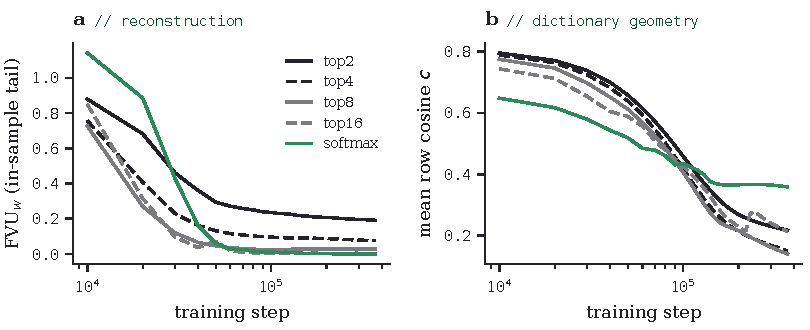
\includegraphics[width=\linewidth]{figures/fig-sweep-curves.pdf}
\caption{The selection sweep's \texttt{\_shm} arms over training:
(a) $\fvu$ on the (in-sample) tail, scored from each checkpoint, and
(b) mean within-head row cosine $\bar\kappa$. The soft arm's $\bar\kappa$ flattens near 0.36 while its
error keeps falling; the hard arms keep decorrelating.}
\label{fig:sweep-curves}
\end{figure}

\paragraph{The last layer is inert once the error is small.} Collinearity
falls monotonically with depth in every hard arm, but soft arms spike at
the last layer (\texttt{softmax\_shm} layer 4: $\bar\kappa{=}0.799$, effective rank
1.54). \texttt{lastlayer.py} ablates the final layer's heads two ways:
uniform (emit the mean atom) and zero (emit nothing):

\begin{center}\small
\begin{tabular}{@{}llrrrrr@{}}
\toprule
arm & select & L4 $\bar\kappa$ & L4 eff & \stackhead[r]{prefix $\fvu$\\before L4} & L4 adds & zero-ablate \\
\midrule
top1         & top1    & $+0.246$ & 10.60 & 0.7511 & $+4.3\%$  & $+4.5\%$ worse \\
top2\_shm    & top2    & $+0.188$ & 14.89 & 0.2378 & $+19.7\%$ & $+24.5\%$ worse \\
top8\_shm    & top8    & ---      & ---   & 0.0304 & $+5.5\%$  & $+5.8\%$ worse \\
top16\_shm   & top16   & $+0.433$ & 3.46  & 0.0043 & $+0.0\%$  & $+0.0\%$ \\
softmax      & softmax & $+0.263$ & 6.00  & 0.0023 & $-1.2\%$  & $-1.1\%$ better \\
softmax\_shm & softmax & $+0.799$ & 1.54  & 0.0007 & $-1.9\%$  & $-1.8\%$ better \\
\bottomrule
\end{tabular}
\end{center}

The last layer's contribution tracks the error left before it, not its
collinearity: \texttt{softmax}'s layer 4 is not collapsed ($\bar\kappa{=}0.263$)
and is just as useless. Below a prefix $\fvu$ of about 0.005 the final
layer is inert or mildly harmful --- which accounts for
\texttt{resid\_nc}'s ``mildly harmful'' layer 4 (prefix 0.0051) without
appeal to its frozen heads. The two collapses end differently:
\texttt{top16\_shm}'s layer 4 shrank its norms to 4\% of the other
layers' and emits nothing; \texttt{softmax\_shm}'s is collinear at
near-equal magnitude, emits a near-constant vector, and removing it
helps --- a small overfit, not a useful bias.

\paragraph{Partitions barely beat a plain smoother.} The noise2self score
that $\mathrm{L2}_{\mathrm{pwak}}$ would train can be read held out
(Figure~\ref{fig:selection}, \texttt{selection.py}): how well a head's
co-classified neighbors predict a row's input, against the same heat
kernel with every row in one cell. No arm of the sweep trained with the
statistic. A head's partition improves on that smoother by at most 0.020,
at layer 0 (\texttt{top4\_shm}), by at most 0.005 at layers 1--3, and by
0.031 at layer 4 only in \texttt{softmax}, where the layer is inert
anyway; a random partition with matched cell sizes is never better than
the smoother, and a one-entry code (\texttt{top1}) is worse than it above
layer 0. Since the score is not $\mathcal{J}$-invariant (Appendix~\ref{app:methods}),
the permuted partition is a floor only for partitions that ignore the
input: a partition computed from the input, trained or not, can gain on
it without clustering anything. One seed per arm; these runs trained on
the evaluation tail.

\paragraph{Under a $\mathcal{J}$-invariant score, partitions show no more
than locality.} The split form (Appendix~\ref{app:methods}) on
\texttt{ste\_h76\_init01}, all 76 heads per layer, settles both
confounds. It selects a bandwidth of 0.05 at layers 0 and 4 and 0.03 at
layers 1--3, and under it the layer-0 smoother at 0.05 scores 0.112
below the smoother at Figure~\ref{fig:selection}'s 0.2, more than any
head or gate gains at 0.2 (at most 0.060). A random-projection head is a
locality-sensitive hash~\cite{harpeled2012}: the chance it puts two rows
in one cell falls as the angle between them grows, so gating the heat
kernel by it sharpens the kernel the way a smaller bandwidth does. At a
bandwidth of 0.2 one random head gains 0.017 over the smoother under the
leave-one-out score and nothing under the split form ($-0.001$), so its
gain was the leak, while the joint gate of eight keeps 0.042 and the
collision kernel 0.047: they sharpen a kernel that is too flat. At the
selected bandwidth single trained heads score worse than the smoother at
every layer (by 0.040 at layer 0, 0.065--0.069 at layers 1--3 and 0.030
at layer 4), as single random heads do (0.030 and 0.063--0.068), and the
layer's joint gate of trained heads gains 0.034 at layer 0 and
0.005--0.006 above it, where the random collision kernel gains 0.039 and
0.005--0.009. Trained heads read every coordinate, so these comparisons
use the leave-one-out form; against random-projection heads, trained
partitions show nothing beyond locality. On isotropic rows the split
form holds its floor down to a bandwidth of 0.05, while the
leave-one-out form falls below it by 0.010 at 0.2 and 0.090 at 0.02,
which is its leak. One seed (\texttt{selection.py --jinv}).

\begin{figure}[tp]
\centering
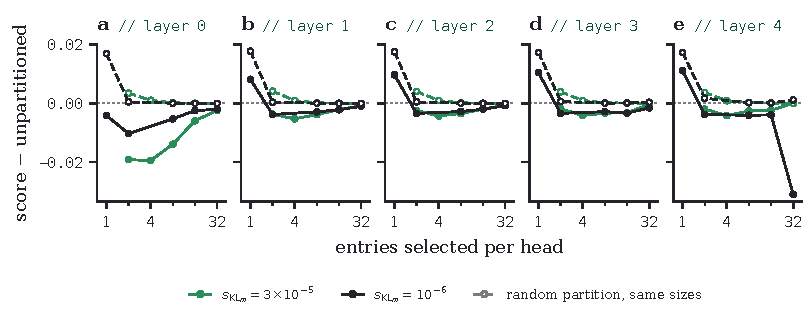
\includegraphics[width=\linewidth]{figures/fig-selection.pdf}
\caption[Held-out noise2self score against the selection
rule]{\textbf{Partitions barely beat a plain smoother.} The selection
	sweep's held-out noise2self score per layer, against the number of
	entries each head selects (1 is argmax, 32 is softmax), less the same
	run's score with every row in one cell (below 0 the partition helps),
	for the two mean-entropy bonus settings. Filled: the heads'
	partitions, mean over heads; hollow, dashed: the same assignments with
	the rows permuted, a random partition with matched cell sizes. Heat
	kernel of bandwidth 0.2 on the layer's input, batches of 2{,}048 rows.
	One seed per arm, in-sample tail.}
\label{fig:selection}
\end{figure}

\subsection{Classifier geometry from the weights}
\label{sec:bilinspec}

Each classifier logit is one bilinear pair,
$(\mathbf{w}\cdot\mathbf{u})(\mathbf{v}\cdot\mathbf{u})$, so
$\lvert\cos\angle(\mathbf{w},\mathbf{v})\rvert$ says what kind of feature it is:
near 1 the form is rank 1, proportional to $(\mathbf{w}\cdot\mathbf{u})^2$,
even in $\mathbf{u}$ and so blind to the sign of the input along
$\mathbf{w}$; near 0 it is a saddle, which sees whether its two
projections agree in sign but is just as even, since
$(\mathbf{w}\cdot(-\mathbf{u}))(\mathbf{v}\cdot(-\mathbf{u})) =
(\mathbf{w}\cdot\mathbf{u})(\mathbf{v}\cdot\mathbf{u})$ on the semantic
coordinates. Rank changes the shape of the region a feature responds to,
not its sign-blindness, which only the constant coordinate breaks
(protocol in Appendix~\ref{app:methods}). Figure~\ref{fig:bilinspec} reads
it from the weights of the softmax stack (\texttt{resid\_nc}) and the
hard-code stack (\texttt{ste\_h76\_init01}).

\textbf{The softmax stack goes rank 1; the hard-code stack mostly does
not.} At the final checkpoint the softmax stack's median
$\lvert\cos\angle\rvert$ is 0.94 in layer 1 and 0.52--0.80 in layers 2--3, where
the hard-code stack's layers 1--3 stay at 0.10--0.16, against 0.021 for a
random pair. Layer 0 sits at 0.54--0.64 in both, and the softmax stack's
layer 4 falls to 0.18. The alignment is learned late: every layer starts
at the random floor; the softmax stack's leave it between 30k and 50k
steps, as its temperature anneal ends, and the hard-code stack's only from
80k (layer 0) and 220k (layers 3--4), with layers 1--2 above 0.05 only at
the last checkpoint. The dominant eigenvalue is negative for 63--98\% of
the softmax stack's features and 97--99\% of the hard-code stack's, so a
rank-1 feature scores high where the input is orthogonal to $\mathbf{w}$,
not along it: the quadratic invariances that bilinear layers learn in
place of constants~\cite{pearce2025}. The constant coordinate can break the sign-blindness of a
rank-1 feature for inputs weakly aligned with $\mathbf{w}$: in the softmax
stack's layers 1--4 its weight is 0.18--0.24 of the rest of $\mathbf{w}$,
in the hard-code stack's 0.017--0.025. One seed per run; weights only.

\begin{figure}[tp]
\centering
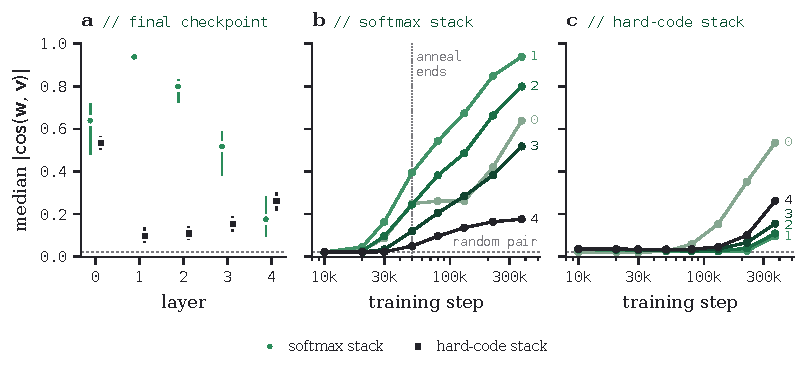
\includegraphics[width=\linewidth]{figures/fig-bilinspec.pdf}
\caption[Classifier geometry from the weights]{\textbf{The softmax
	stack's classifier features go rank 1; the hard-code stack's mostly do
	not.} Median $\lvert\cos\angle(\mathbf{w},\mathbf{v})\rvert$ of each layer's
	bilinear feature pairs (\texttt{bilinspec.py}), 1 for a rank-1 feature.
	(a) The final checkpoint by layer, with interquartile ranges: the softmax
	stack (\texttt{resid\_nc}, step 372.6k) and the hard-code stack
	(\texttt{ste\_h76\_init01}, step 369.5k). (b, c) Over training, one line
	per layer, numbered at its end; the softmax stack's temperature anneal
	ends at 50k, and the hard-code stack's temperature is constant. Dashed:
	the median for a random pair in the 1024-dimensional semantic block,
	0.021. One seed per run.}
\label{fig:bilinspec}
\end{figure}


\end{document}
